% Do not change document class, margins, fonts, etc.
\documentclass[a4paper,oneside,bibliography=totoc]{scrbook}

% ---- FAST-DRAFT TOGGLE ----
% Uncomment the next line to skip embedding images (~8x faster builds while editing).
% Figures show as labelled boxes. Re-comment it before producing the final PDF.
%\PassOptionsToPackage{draft}{graphicx}

% some useful packages (add more as needed)
\usepackage[utf8]{inputenc}
\usepackage{graphicx}
\usepackage{subcaption}
\usepackage{latexsym}
\usepackage{amsmath}
\usepackage{longtable}
\usepackage{caption}
\usepackage{booktabs}
\usepackage{amssymb}
\usepackage{tabularx}
\usepackage{algorithm} % you can modify the algorithm style to your liking
\counterwithin{algorithm}{chapter} % so that algorithms have chapter numbers as well
\usepackage{algorithmic}
\usepackage{csquotes}
\renewcommand{\algorithmiccomment}[1]{\hfill\textit{// #1}}
\usepackage[usenames,dvipsnames]{xcolor}
\usepackage[hidelinks]{hyperref} % black, un-boxed links for printing (was colorlinks,citecolor=Green)
\usepackage{lipsum} % you do not need this
\usepackage{multirow}
\usepackage{tikz}
\usetikzlibrary{arrows.meta,positioning}
% chicago citation style
\usepackage{natbib}
\bibliographystyle{chicagoa}
\setcitestyle{authoryear,round,semicolon,aysep={},yysep={,}} \let\cite\citep

% example enviroments (add more as needed)
\newtheorem{definition}{Definition} \newtheorem{proposition}{Proposition}

% marker for results that still have to be produced / exported
\newcommand{\missing}[1]{\textcolor{red}{\textbf{[MISSING:} #1\textbf{]}}}

% SPARQL query block: monospace code cell, line breaks via \\, indentation via \quad.
% Wrapped in a minipage so that \\ is a real line break (not a table row terminator)
% and the font/size stays contained to the cell.
\newcommand{\sparql}[1]{%
  \begin{minipage}[t]{\linewidth}%
  \ttfamily\scriptsize\setlength{\parindent}{0pt}\raggedright
  #1%
  \end{minipage}}

\begin{document}

\frontmatter \subject{Master Thesis} % change to appropriate type
\title{Schema-based pre-training for
RDF2Vec}
\author{Erblina Qeli\\
  (matriculation number 1980490)} \date{June 18, 2026}
\publishers{{\small Submitted to}\\
  Data and Web Science Group\\
  Prof.\ Dr.\ Heiko Paulheim\\
  University of Mannheim\\}
\maketitle

\chapter{Abstract}

\emph{RDF2Vec} embeds a knowledge graph by running random walks over its instance
graph and training a skip-gram language model on the resulting token sequences. It
does not take the schema as a separate input: class hierarchies, domains, and
ranges shape the embeddings only indirectly, and only to the extent the walked
graph already exposes them. This thesis asks whether supplying the schema
explicitly, through the initialization, gives RDF2Vec a useful starting point, and
what decides when it helps. Building on schema-based protograph pre-training, we
propose a \emph{concept-bound initialization} that assembles, for each entity, an
explicit one-hop schema feature from its (relation, neighbour-class) pairs and its
direction-tagged edge counts, rescales every vector to a shared norm, and
fine-tunes at a reduced rate so the transferred structure survives. We compare it
against the classic transfer, which copies only an entity's own class vectors, and
against vanilla RDF2Vec.

Two factors determine whether schema-based initialization is beneficial. 
The first is \emph{what} information the initialization encodes, rather than simply 
\emph{how much} schema information is pre-trained. 
This becomes visible on the controlled synthetic benchmark, where the random walks
 contain no explicit type information. For relation-centric test cases, transferring
  only an entity's own class vectors provides little or no useful signal, because the 
  target concept is defined by relational structure rather than by the entity type 
  alone. In contrast, the concept-bound initialization directly encodes relation--neighbour-class pairs and direction-aware edge counts. On these tasks, it improves mean accuracy by about \textbf{28\%} over vanilla RDF2Vec. Since the improvement is already present at the first epoch, it is mainly read from the initialization itself rather than learned during fine-tuning.

The second factor is whether the transferred signal remains numerically stable on a real graph. On DBpedia, the ranking reverses: the same edge-count channel that gives concept-bound initialization its synthetic advantage can also dominate the vector space. Without normalization, high-degree hub entities obtain very large vector norms. Under the reduced fine-tuning rate, these embeddings become difficult to move, so the uncapped variant effectively freezes some of the most influential rows and performs worst overall. Applying a simple per-row norm cap resolves this failure mode. It preserves the useful count-based signal while preventing hubs from overwhelming the embedding space, turning the weakest variant into the strongest and increasing the mean accuracy from \textbf{0.808} to \textbf{0.850}.

% table of contents
\begingroup%
\hypersetup{hidelinks}% disable link color in TOC only
\tableofcontents%
\endgroup

% none of the things below is needed, but you may add them if you feel that they
% are helpful for your work \listofalgorithms \listoffigures \listoftables
% \listtheorems{definition} \listtheorems{proposition}


% okay, start new numbering ... here is where it really starts
\mainmatter


\chapter{Introduction}
\label{ch:intro}

Knowledge graphs represent real-world entities and their relations in a
structured, machine-readable form. They are built from RDF triples of the form
(subject, relation, object) and support applications such as semantic search,
recommendation~\cite{wang_kgat_2019}, question answering~\cite{lan_survey_2021},
and data integration~\cite{hogan_introduction_2022}. To use them in machine
learning pipelines, knowledge graph embedding methods map entities and relations
to continuous vectors that downstream tasks such as link prediction, clustering,
and node classification can read~\cite{wang_knowledge_2017}.\footnote{The code
and data to reproduce the experiments are available at
\url{https://github.com/erblinaqeli/schema-pretraining-rdf2vec}.}

How much semantic meaning these vectors actually capture is unclear. Embeddings
often learn structural regularities without representing the underlying meaning
of entities and relations~\cite{jain2021semantics}. The problem is sharp for
methods trained on instance-level structure alone, because a knowledge graph
also has a schema that states classes, subclass relations, and the domains and
ranges of relations. RDF2Vec is a prominent example: it extracts random walks
from the instance graph and trains a skip-gram language model on
them~\cite{groth_rdf2vec_2016}, and never reads the schema. The conceptual
distinctions encoded there are left out of training.

A recent approach, MASCHInE, addresses this by compiling the schema into a small
graph called a protograph~\cite{hubert2023maschine}. The protograph holds
abstract entities for classes and triples derived from domain, range, and
subclass declarations. Embeddings are pre-trained on it and then transferred to
initialize the instance model before fine-tuning. MASCHInE improved semantic
quality for several link-prediction embedding models, but it was not designed for
RDF2Vec, which is built on random walks and a language-model objective rather
than on a triple-scoring function. This thesis carries the idea to RDF2Vec and
asks a sharper question. Can the schema give RDF2Vec a useful starting point, and
what decides when it pays off?

To study this we build two artifacts. The first is an RDF-schema view of the DLCC
benchmark, which probes which description-logic class patterns an embedding can
represent through test cases that isolate outgoing relations, incoming relations,
qualified restrictions, and cardinalities~\cite{portisch_dlcc_2022}. We add
schema-specific test cases tc13--tc15 and three protograph constructions, P1, P2,
and P3, that give every class a pre-trained code. The second is the
\emph{concept-bound} initialization. Rather than hoping that fine-tuning will
combine own-class vectors into useful features, it builds those features
directly: it binds each entity to its (relation, neighbour-class) pairs and to
its direction-tagged edge counts, rescales every vector to a shared target norm,
and fine-tunes at a protected learning rate so the transferred structure
survives. We compare it against the classic transfer (\texttt{most\_specific}),
which only copies own-class vectors, and against vanilla RDF2Vec with random
initialization.

On the synthetic DLCC benchmark the schema helps, but its value is set by
\emph{what} the initialization encodes, not by how much schema is pre-trained. On
the relation-centric test cases tc07--tc12, where own-class vectors carry no
signal, the concept-bound initialization lifts mean accuracy by about $0.28$ over
vanilla, while the classic transfer helps only where the label is the entity's
own class. The gain is an initialization effect: the bound signal is already
readable at the first epoch, and protected fine-tuning keeps it.

On a real graph a second condition appears. The gain survives only if fine-tuning
can still move what was encoded. On DBpedia the cardinality channel writes edge
counts into vector magnitude, and a few high-degree hubs reach very large norms
that a protected step cannot turn, so those rows freeze and the uncapped
concept-bound initialization finishes worst end-to-end. The fix is one line.
Capping the norm on those few thousand rows turns the worst variant into the best
overall (mean $0.808 \rightarrow 0.850$). On standard downstream tasks the DLCC
ranking does not carry over, so a high DLCC score does not predict downstream
quality.

In summary, this thesis adapts schema-based protograph pre-training to RDF2Vec
and extends DLCC with schema-specific test cases; it introduces the concept-bound
initialization, which encodes relation--class bindings and cardinalities
explicitly; it shows on a controlled benchmark that what the initialization
encodes matters more than how much schema is pre-trained; and it identifies, on a
real graph, a single robust component, a per-row norm cap, that keeps a
schema-bound initialization from freezing and lets it stay competitive
end-to-end.

The remainder of this thesis is structured as follows.
Chapter~\ref{ch:background} introduces knowledge graphs, RDF2Vec, the DLCC
benchmark, and schema-based pre-training. Chapter~\ref{ch:classic} develops
schema-based pre-training for RDF2Vec, from the protograph constructions and the
classic transfer to the proposed concept-bound initialization.
Chapter~\ref{ch:experiments} reports the evaluation on the synthetic and DBpedia
DLCC benchmarks and on downstream tasks. Chapter~\ref{ch:conclusion} summarizes
the findings, limitations, and directions for future work.

%=====================================================================
\chapter{Literature Review}
\label{ch:related_work}
\label{ch:background}

This chapter introduces the four building blocks of this thesis. We first
recall knowledge graphs and the distinction between their instance level and
their schema level. We then describe RDF2Vec, the embedding method we build on,
and the DLCC benchmark, which we use as the measuring instrument throughout the
thesis. Finally, we review schema-based pre-training, in particular the
MASCHInE approach whose adaptation to RDF2Vec is the starting point of our
work, and summarize the gap this thesis addresses.

\section{Knowledge Graphs and RDF}
\label{sec:lit_kg}

Knowledge graphs are graph-structured representations of data that aim to
capture and convey knowledge about real-world entities and their relations.
Although there is no single universally accepted definition of a knowledge
graph, common characteristics include the representation of entities and
interrelations in a graph, together with a schema that defines possible classes
and relations~\cite{paulheim_knowledge_2016,hogan_introduction_2022}. Since
knowledge graphs can be based on different graph-based data models, this thesis
focuses on RDF-based knowledge graphs.

In RDF, information is represented as triples $(s, p, o)$, where $s$ is the
subject, $p$ is the predicate, and $o$ is the object~\cite{cyganiak2014rdf}. A
set of RDF triples therefore forms a directed labeled graph: subjects and
objects correspond to nodes, while predicates correspond to labeled edges
between them. In the context of this thesis, predicates are also referred to as
relations, since they define the edge type between two nodes in the graph.

For example, a triple of the form
\[
(\text{LeBron James}, \text{team}, \text{Los Angeles Lakers})
\]
states that the subject \textit{LeBron James} is connected to the object
\textit{Los Angeles Lakers} by the predicate \textit{team}. More generally, an
RDF graph may contain entities such as persons, cities, or organizations, and
relations such as \textit{bornIn}, \textit{locatedIn}, or \textit{worksFor}.

A distinction can be made between the instance graph and the ontology or schema
graph. The instance graph contains concrete entities and factual statements
about them, represented as RDF triples~\cite{hogan_introduction_2022}. For
example, it may contain information about specific people, cities, movies, or
organizations. The ontology or schema graph, in contrast, describes the
structure of the data at a more abstract level. In RDF Schema, this includes
class membership via \texttt{rdf:type}, class hierarchies via
\texttt{rdfs:subClassOf}, and domain and range constraints for properties via
\texttt{rdfs:domain} and \texttt{rdfs:range}~\cite{cyganiak2014rdf,brickley_rdfs_2014}.

Classes are used to group entities with similar meaning. For example,
\textit{LeBron James} may be an instance of the class \textit{Person}, while
\textit{Los Angeles Lakers} may be an instance of the class \textit{SportsTeam}.
In RDF, this is usually expressed using \texttt{rdf:type}. A statement such as
\[
(\text{LeBron James}, \texttt{rdf:type}, \text{Person})
\]
means that \textit{LeBron James} belongs to the class \textit{Person}.

Ontologies can also define subclass relations. A subclass relation states that
one class is more specific than another class. For example,
\textit{BasketballTeam} may be a subclass of \textit{SportsTeam}. This means
that every basketball team is also a sports team. Such class hierarchies are
important because they encode semantic information that may not be directly
visible from instance triples alone.

In addition to classes and subclasses, RDF schemas can define domains and
ranges of relations. The domain of a relation specifies which class is expected
to appear as the subject of that relation, while the range specifies which class
is expected to appear as the object. For example, if the relation \textit{team}
has domain \textit{Person} and range \textit{SportsTeam}, then a triple using
this relation is expected to connect a person to a sports team:
\[
(\text{Person}, \text{team}, \text{SportsTeam})
\]
This kind of schema information is central to this thesis. While the instance
graph shows concrete facts, the schema graph provides more general knowledge
about how entities and relations are expected to interact. The main idea
investigated in this work is whether such schema-level information can be used
to initialize or improve RDF2Vec embeddings learned on the instance graph.

Knowledge graph embedding (KGE) methods map entities and relations into a
continuous vector space such that graph structure is (approximately)
preserved~\cite{wang_knowledge_2017}. A large family of models is trained for link prediction with
triple-scoring objectives \cite{ji_survey_2022, sardina_survey_2024}. A
recurring criticism of this line of work is that good link-prediction scores do
not imply that the embeddings represent the \emph{semantics} of entities;
\citet{jain2021semantics} show that embeddings often reflect structural
regularities rather than conceptual meaning. This observation motivates both
benchmarks that probe semantic capabilities directly
(Section~\ref{sec:lit_dlcc}) and training procedures that inject schema
knowledge explicitly (Section~\ref{sec:lit_pretraining}).

\section{RDF2Vec}
\label{sec:lit_rdf2vec}

RDF2Vec is a knowledge graph embedding approach that adapts word embedding
models to RDF graphs~\citep{ristoski2019rdf2vec,paulheim_embedding_2023,portisch_rdf2vec_family_2024}.
Its main intuition follows the distributional idea behind Word2Vec: tokens that
occur in similar contexts should obtain similar vector representations
(\citealp{mikolov_efficient_2013}; \citealp{mikolov_distributed_2013}). In natural language,
the tokens are words and the contexts are neighbouring words in sentences. In
RDF2Vec, the tokens are entities and predicates, and the contexts are obtained
from graph walks.

\paragraph{Random-walk corpus.}
RDF2Vec first transforms an RDF graph into a corpus of token sequences. This is
done by performing random walks over the graph. A walk alternates between entity
and predicate tokens, and can therefore be treated similarly to a sentence in
natural language. A Word2Vec model is then trained on the generated walk corpus.
The resulting embeddings represent entities and predicates according to the graph
contexts in which they occur.

\begin{figure}[htbp]
\centering
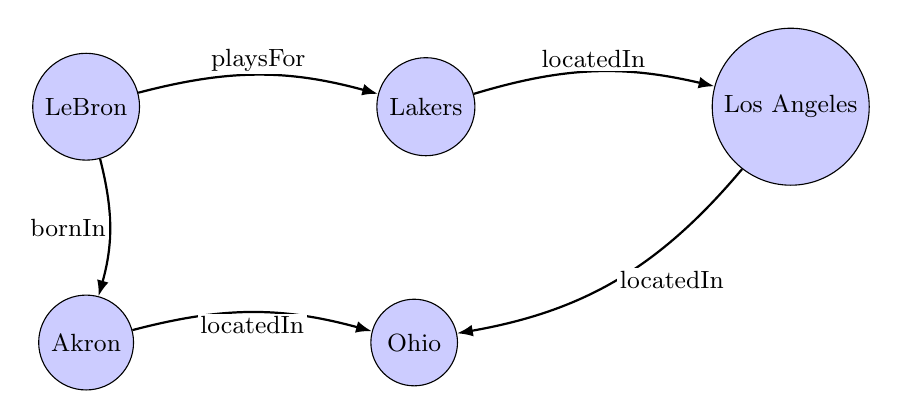
\begin{tikzpicture}[
entity/.style={
circle,
draw,
fill=blue!20,
minimum size=1.1cm,
font=\small
},
edge/.style={
-{Latex[length=2mm]},
thick,
bend left=15
},
label/.style={
font=\small,
fill=white,
inner sep=1pt
}
]

\node[entity] (lebron) {LeBron};
\node[entity, right=3.0cm of lebron] (lakers) {Lakers};
\node[entity, right=3.0cm of lakers] (la) {Los Angeles};
\node[entity, below=1.7cm of lebron] (akron) {Akron};
\node[entity, right=3.0cm of akron] (ohio) {Ohio};

\draw[edge] (lebron) to node[label, above] {playsFor} (lakers);
\draw[edge] (lakers) to node[label, above] {locatedIn} (la);
\draw[edge] (lebron) to node[label, left] {bornIn} (akron);
\draw[edge] (akron) to node[label, below] {locatedIn} (ohio);
\draw[edge] (la) to[bend left=20] node[label, right] {locatedIn} (ohio);

\end{tikzpicture}
\caption{Example RDF graph used to illustrate RDF2Vec random walks.}
\label{fig:rdf2vec_example}
\end{figure}

For example, from the graph in Figure~\ref{fig:rdf2vec_example}, RDF2Vec
may generate walks such as:
\[
\text{LeBron} \rightarrow \text{playsFor} \rightarrow \text{Lakers}
\rightarrow \text{locatedIn} \rightarrow \text{Los Angeles}
\]
and
\[
\text{LeBron} \rightarrow \text{bornIn} \rightarrow \text{Akron}
\rightarrow \text{locatedIn} \rightarrow \text{Ohio}.
\]
Each element in such a walk is treated as a token. The graph structure is
therefore converted into co-occurrence information: entities and predicates that
appear in similar walk contexts receive similar training signals.

\paragraph{Word2Vec training.}
In this thesis, RDF2Vec is trained with the skip-gram architecture and negative
sampling, a configuration commonly known as skip-gram with negative sampling
(SGNS); accordingly, when we later refer to RDF2Vec's training objective,
updates, or weight matrices, we mean this SGNS model. In the skip-gram model, a
center token is used to predict nearby tokens
within a fixed context window~\citep{mikolov_efficient_2013}. Applied to
RDF2Vec, this means that an entity or predicate occurring in a random walk is
trained to predict the surrounding entities and predicates in that walk. The
window size controls how much local graph context contributes to the embedding:
a larger window creates more training pairs, but also increases the computational
cost.

Skip-gram training maintains two sets of vectors. The first set contains input
vectors for the observed tokens, while the second set contains output, or
context, vectors used when predicting neighbouring tokens
\citep{mikolov_distributed_2013}. The full softmax objective over the complete
vocabulary is expensive, so skip-gram is commonly trained with negative sampling.
For each observed token--context pair, the model learns to distinguish the true
context token from randomly sampled negative tokens
\citep{mikolov_distributed_2013}. After training, the RDF2Vec representation of
an entity is usually taken from the learned input-vector matrix.

This distinction is important for schema-based initialization. Initializing an
entity vector changes the starting point of the input embedding that is later
fine-tuned on instance walks. However, the output or context-side parameters also
influence the first skip-gram updates. Therefore, when schema-derived vectors are
transferred before instance-level RDF2Vec training, one must decide whether the
initialization is applied only to the input embeddings or also mirrored to the
negative-sampling output vectors. This implementation detail becomes relevant in
later chapters, where we analyze how much of the protograph signal survives
fine-tuning.

\paragraph{RDF2Vec as graph representation learning.}
As a result of this training process, entities with similar graph neighbourhoods
are expected to receive similar embeddings. For instance, two basketball players
may be connected to similar types of entities, such as teams, positions, leagues,
or places of birth. Even if they are not directly connected, their random walks
may contain similar patterns, causing their embeddings to be placed close to each
other in the vector space. In this way, RDF2Vec captures local graph structure
through co-occurrence patterns in random walks.

The learned embeddings can be used as input features for downstream tasks such
as node classification, clustering, or link prediction. In this thesis, RDF2Vec
embeddings are evaluated using the DLCC benchmark, which tests which kinds of
logical graph patterns are captured by the embeddings.

However, standard RDF2Vec mainly learns from the graph on which the walks are
performed. In the setting considered in this thesis, these walks are generated
from the instance graph. RDF2Vec therefore observes concrete graph
neighbourhoods, but does not explicitly exploit schema-level information such as
class hierarchies, domains, and ranges. This motivates the central question of
this thesis: whether initializing RDF2Vec with embeddings learned from a
schema-derived protograph can improve the semantic information captured by the
final instance embeddings.

\section{Benchmarking Expressivity of Embeddings: DLCC}
\label{sec:lit_dlcc}

Evaluating what knowledge graph embeddings actually capture has motivated
several benchmarks for node classification and related tasks. General-purpose
suites such as gEval~\cite{pellegrino_configurable_2019,pellegrino_geval_2020} aggregate many heterogeneous
downstream tasks (classification, clustering, regression, entity relatedness),
and resources such as kgbench~\cite{bloem_kgbench_2021} provide standardized
node classification datasets at scale. These benchmarks measure overall
downstream utility, but they do not isolate \emph{which} structural or logical
patterns an embedding encodes. DLCC is designed for exactly this diagnostic
purpose, which is why we adopt it as the measuring instrument in this thesis.

The DLCC benchmark, short for \emph{Description Logic Class Constructors},
analyzes which kinds of graph patterns knowledge graph embeddings can
represent~\cite{portisch_dlcc_2022}. Instead of evaluating embeddings only on
a general downstream task, DLCC defines binary node classification tasks from
Description Logic (DL) class constructors. Positive examples satisfy the
corresponding graph pattern, while negative examples do not.

A DL class constructor describes a class through a structural condition in the
graph. For example, a class may contain all entities with a certain outgoing
relation, all entities connected to a specific individual, all entities
connected to an object of a given type, or all entities with at least two
relations of a certain kind. The embeddings of positive and negative entities
are then used as input to classifiers; good classification performance
indicates that the embedding captures information relevant to the tested
constructor.

DLCC provides two complementary gold standards: one based on
DBpedia~\cite{lehmann_dbpedia_2015} and one based on synthetic data. The DBpedia benchmark evaluates embeddings on a
real-world knowledge graph, using SPARQL queries to generate positives,
negatives, and hard negatives across several domains. However, real-world graphs
contain correlations, so high accuracy may sometimes come from related co-occurring
patterns rather than from the intended DL constructor itself.

For this reason, the synthetic DLCC benchmark is especially useful in this
thesis. It creates controlled graphs where the target constructors are inserted
explicitly and additional triples are added only if they do not accidentally
create new positive examples. This makes the synthetic benchmark a cleaner
setting for testing which structural patterns RDF2Vec can encode, while the
DBpedia benchmark serves as a realistic counterpart.

Table~\ref{tab:dlcc-test-cases} summarizes the twelve original DLCC test cases.
They cover relation existence, relations to particular individuals (both via a
fixed relation and via any relation), qualified restrictions, and (qualified)
cardinality patterns.
\begin{table}[htbp]
\centering
\caption{Overview of the DLCC test cases used in this thesis. TC01--TC12 are
taken from the original DLCC benchmark~\cite{portisch_dlcc_2022}; TC13--TC15 are
schema-oriented extensions introduced in this thesis.}
\label{tab:dlcc-test-cases}
\footnotesize
\renewcommand{\arraystretch}{1.25}
\begin{tabularx}{\textwidth}{@{}c >{\raggedright\arraybackslash}p{0.38\textwidth} >{\raggedright\arraybackslash}X@{}}
\toprule
\textbf{TC} & \textbf{Pattern} & \textbf{What it tests} \\
\midrule

TC01 &
$\exists r.\top$
& Whether an entity has at least one outgoing edge with relation $r$. \\

TC02 &
$\exists r^{-1}.\top$
& Whether an entity has at least one incoming edge with relation $r$. \\

TC03 &
$\exists r.\top \sqcup \exists r^{-1}.\top$
& Whether an entity has relation $r$ in either outgoing or incoming direction. \\

TC04 &
$\exists R.\{e\} \sqcup \exists R^{-1}.\{e\}$
& Whether an entity is connected to a particular entity $e$ by any relation, in either direction. \\

TC05 &
$\exists R_1.(\exists R_2.\{e\}) \sqcup \exists R_1^{-1}.(\exists R_2^{-1}.\{e\})$
& Whether an entity is connected to a particular entity $e$ through a two-hop path of arbitrary relations, either in the forward or inverse direction. \\

TC06 &
$\exists r.\{e\}$
& Whether an entity has a particular relation $r$ to a particular entity $e$. \\

TC07 &
$\exists r.T$
& Whether an entity has relation $r$ to an entity of type $T$. \\

TC08 &
$\exists r^{-1}.T$
& Whether an entity has an incoming relation $r$ from an entity of type $T$. \\

TC09 &
$\geq 2r.\top$
& Whether an entity has at least two outgoing $r$-edges to distinct entities. \\

TC10 &
$\geq 2r^{-1}.\top$
& Whether an entity has at least two incoming $r$-edges from distinct entities. \\

TC11 &
$\geq 2r.T$
& Whether an entity has at least two outgoing $r$-edges to distinct entities of type $T$. \\

TC12 &
$\geq 2r^{-1}.T$
& Whether an entity has at least two incoming $r$-edges from distinct entities of type $T$. \\

\midrule

TC13 &
$D \sqcap \exists p.R_1$ vs. $D \sqcap \exists p.R_2$
& Range-side subclass distinction: subjects have the same domain class $D$ and relation $p$, but the object belongs to different sibling subclasses $R_1$ or $R_2$ of the declared range $R$. \\

TC14 &
$D_1 \sqcap \exists p.R$ vs. $D_2 \sqcap \exists p.R$
& Domain-side subclass distinction: subjects belong to different sibling subclasses $D_1$ or $D_2$ of the declared domain $D$, while the relation and range side are held fixed. \\

TC15 &
$D_{\mathrm{sub}} \sqcap \exists p.R_{\mathrm{sub}}$ vs. $D_{\mathrm{sub}} \sqcap \exists p.W$
& Schema-valid versus schema-invalid filler: the positive object belongs to a subclass of the declared range $R$, while the negative object belongs to a class $W$ outside the declared range. \\

\bottomrule
\end{tabularx}
\end{table}

Here, $r$ denotes a fixed relation, $R$ an arbitrary relation, $e$ a fixed
individual, $T$ a class, and $\top$ an unrestricted filler; the superscript
${}^{-1}$ marks the inverse (incoming) direction. The distinction between $T$
and $\top$ matters: TC01~($\exists r.\top$) only requires an outgoing
$r$-edge, whereas TC07~($\exists r.T$) additionally requires that edge to point
to an entity of type~$T$.

An important detail of the synthetic gold standard is that the generated
instance graph (\texttt{graph.nt}) contains \emph{no} \texttt{rdf:type}
triples: all class information lives in the accompanying ontology file. This
construction makes DLCC a sharp instrument for our research question, because
any class-dependent signal in the embeddings must have entered through
schema-aware training rather than through ordinary instance walks.

\section{Knowledge Graph Embeddings and Schema-Based Pretraining}
\label{sec:lit_pretraining}

Recall from Section~\ref{sec:lit_kg} that knowledge graph embedding methods place
entities and relations in a continuous vector space, so that entities that play
similar roles in the graph end up close together. Most KGE models are trained for
\emph{link prediction}: a scoring function rates how plausible a triple is, and
training pushes the scores of real triples above those of corrupted ones
\citep{ji_survey_2022,sardina_survey_2024}. As discussed there, a high
link-prediction score does not, on its own, mean that the embeddings capture the
semantic meaning of the entities they represent \citep{jain2021semantics}.

One way to address this limitation is to incorporate schema information into
representation learning. Existing schema-aware KGE methods use this information
in different parts of the training process. Some approaches use type information during negative sampling, so that corrupted triples are more realistic
\citep{arenas_type-constrained_2015}. 
Others modify the loss function with ontological constraints such as domain and range restrictions
\citep{10.1007/978-3-030-77385-4_26,hubert_negatives_2024}, use contrastive learning over explicit negative statements
\citep{sousa_improving_2025},
or extend the model representation with type-level information
\citep{3060832.3061036}.
These methods show that schema information can improve semantic consistency,
but they are often tied to a particular embedding model, loss function, or
training objective.

MASCHInE~\citep{hubert2023maschine} follows a different strategy. Instead of
injecting schema information directly into a specific KGE model, it uses the
schema to construct a separate protograph. The protograph is a small
schema-derived graph whose nodes correspond to classes and whose edges are
derived from domain, range, and subclass information. Embeddings are first
trained on this protograph and are then transferred to the entities of the
instance graph before normal training continues. This makes MASCHInE especially
relevant for this thesis, because the idea of schema-based pretraining is
conceptually model-agnostic and can therefore be investigated for RDF2Vec.

From the ontology, MASCHInE derives protographs using two construction rules.
P1 creates, for every relation $r$ with declared domain $C_d$ and range $C_r$,
the prototriple $(C_d, r, C_r)$. P2 extends this construction by also
considering direct subclasses of the domain and range classes. For a relation
with domain $C_d$, range $C_r$, and direct subclasses
$C'_d \sqsubseteq C_d$ and $C'_r \sqsubseteq C_r$, P2 additionally creates
one-sided subclass prototriples such as $(C'_d, r, C_r)$ and
$(C_d, r, C'_r)$. Thus, P2 produces a larger and more fine-grained
protograph than P1, but may also introduce noisy or overly permissive schema
triples.

After training on the protograph, MASCHInE initializes each instance entity
with the embedding of its corresponding class, or with the mean of several class
embeddings if the entity has multiple most specific classes. Training then
continues on the original instance graph. In this way, schema-level information
is transferred into the initial entity representations before instance-level
training begins.

However, transferring this recipe to RDF2Vec is non-trivial. MASCHInE was
evaluated on triple-scoring KGE models such as TransE, DistMult, ComplEx,
ConvE, and TuckER. RDF2Vec is different: it does not optimize a triple-scoring
objective, but learns from token co-occurrences in random walks. Therefore, it is
not obvious whether protograph embeddings can be injected in the same way,
whether the schema signal survives instance-level fine-tuning, or whether
class-mean initialization is sufficient for DLCC tasks that depend on the classes
of neighbouring entities rather than only on the entity's own class. These
questions define the gap addressed in this thesis.
\subsection{Vector-Symbolic Binding}
\label{sec:lit_vsa}

The method proposed in Section~\ref{sec:concept_bound} also uses an idea from
vector-symbolic architectures (VSAs), also known as hyperdimensional computing. VSAs represent
symbols as high-dimensional vectors and define algebraic operations for combining
such vectors into structured representations~\citep{kleyko_survey_2023}.
The operation that is relevant for this thesis is \emph{binding}: two vectors are
combined into a new vector that represents their association while keeping the
same dimensionality.

This idea is useful for the relation-centric DLCC tasks. A qualified restriction
such as $\exists r.C$ is not only about the presence of relation $r$ or class $C$
individually, but about their combination: an entity must have an $r$-edge to a
neighbour of class $C$. If relation and class vectors are only added separately,
the pairing between them can be lost. For example, an embedding that contains
separate evidence for relation $r$ and class $C$ does not necessarily encode that
$r$ points to an entity of class $C$.

In Section~\ref{sec:binding}, we therefore use the Hadamard product
$\mathrm{emb}(r) \odot \mathrm{emb}(C)$ as a simple binding operation for
relation--class pairs. The resulting vector is used as a feature in the
initialization of an entity embedding. Incoming edges are additionally marked by
applying a fixed permutation to the relation vector before binding, so that
outgoing and incoming uses of the same relation remain distinguishable. This
allows the initialization to encode one-hop schema patterns such as $\exists r.C$
and $\exists r^{-1}.C$ directly, instead of relying on RDF2Vec fine-tuning to
discover them from random-walk co-occurrences.

\section{Summary}
\label{sec:lit_summary}

Knowledge graphs separate cheap-to-state conceptual knowledge (the schema)
from voluminous factual knowledge (the instance graph). In the standard setting considered in this thesis, RDF2Vec is trained on the instance graph and therefore captures schema information only indirectly, if such information is present in the walked graph. DLCC
provides a fine-grained diagnostic of which DL constructors an embedding
captures, and MASCHInE demonstrates that schema-derived protographs are a
viable pre-training corpus for triple-scoring KGE models. What is missing,
and what this thesis contributes, is (i) a systematic adaptation of
protograph pre-training to RDF2Vec, (ii) an analysis of where the classic
transfer succeeds and where it structurally fails on DLCC
(Chapter~\ref{ch:classic}), and (iii) a new initialization that encodes
relation--class bindings and cardinalities explicitly, turning the protograph
embeddings into one-hop schema features (Section~\ref{sec:method_overview}).

%=====================================================================
\chapter{Schema-Based RDF2Vec Pretraining}
\label{ch:classic}
\label{ch:schema_pretraining}

This chapter develops schema-based pre-training for RDF2Vec. We first extend
the DLCC benchmark with three RDF-schema-specific test cases that isolate the
schema distinctions our methods target (Section~\ref{sec:new_tcs}). We then
describe how schema information is turned into a pre-training corpus (the
protograph construction rules), and how the pretrained class and relation
embeddings are transferred to initialize instance entities along the class
hierarchy (Sections~\ref{sec:classic_pipeline} and~\ref{sec:init_strategies}),
together with the structural limitations of this classic transfer
(Section~\ref{sec:classic_limits}). These limitations motivate the proposed
\emph{concept-bound} initialization (Section~\ref{sec:method_overview}), which
assembles the pretrained vectors into an explicit one-hop schema feature per
entity instead of relying on fine-tuning to discover it. We close with the
design choices that are evaluated empirically in
Chapter~\ref{ch:experiments}: the fine-tuning learning rate, protograph
anchoring, initialization noise, the walk budget, and direction-aware
cardinality encoding.

\section{RDF-Schema Specific Extensions of DLCC}
\label{sec:new_tcs}

The original DLCC benchmark (Table~\ref{tab:dlcc-test-cases}) probes generic
graph patterns but does not isolate the schema distinctions (subclass of the
declared domain, subclass of the declared range, and range validity) that
schema-based pre-training is meant to capture. We therefore extend the
synthetic DLCC benchmark with three RDF-schema-specific test cases,
TC13--TC15. Table~\ref{tab:tc13-tc15-motivation} summarizes their purpose and
shows which schema distinction each one is designed to isolate.


\begin{table}[htbp]
  \centering
  \caption{Purpose of the additional synthetic test cases TC13--TC15.}
  \label{tab:tc13-tc15-motivation}
  \small
  \renewcommand{\arraystretch}{1.25}
  \begin{tabularx}{\textwidth}{@{}c >{\raggedright\arraybackslash}X >{\raggedright\arraybackslash}X >{\raggedright\arraybackslash}X@{}}
      \toprule
      \textbf{TC} &
      \textbf{What it checks} &
      \textbf{Example} &
      \textbf{Why it is useful} \\
      \midrule

      TC13 &
      Checks whether the embedding can distinguish which subclass of the declared range appears as the object of a relation. &
      Suppose \texttt{headquarter} has range \texttt{Place}. \newline
      Positive: a company has its headquarter in a \texttt{City}. \newline
      Negative: a company has its headquarter in a \texttt{Country}. \newline
      Both \texttt{City} and \texttt{Country} are subclasses of \texttt{Place}. &
      Tests range-side subclass information. Both objects are schema-valid places, so the task is not just about whether the relation satisfies its declared range. \\

      \addlinespace

      TC14 &
      Checks whether the embedding can distinguish which subclass of the declared domain appears as the subject of a relation. &
      Suppose \texttt{headquarter} has domain \texttt{Organisation}. \newline
      Positive: a \texttt{Company} has a headquarter in a city. \newline
      Negative: a \texttt{SportsClub} has a headquarter in a city. \newline
      Both \texttt{Company} and \texttt{SportsClub} are subclasses of \texttt{Organisation}. &
      Tests domain-side subclass information. Both examples have the same relation pattern, so the task is not just about having a \texttt{headquarter} edge. \\

      \addlinespace

      TC15 &
      Checks whether the embedding can distinguish a schema-valid filler from a filler outside the declared range. &
      Suppose \texttt{birthPlace} has range \texttt{Place}. \newline
      Positive: a person has \texttt{birthPlace} New York City. \newline
      Negative: a person has \texttt{birthPlace} LeBron James. \newline
      New York City is a \texttt{Place}, but LeBron James is a \texttt{Person}. &
      Tests whether schema pretraining helps the model represent range validity. The subject type and relation are fixed, but the negative object violates the expected range of the relation. \\

      \bottomrule
  \end{tabularx}
\end{table}

\section{Protograph Construction}
\label{sec:classic_pipeline}
\label{sec:protograph_construction}

Schema-based pre-training compiles the ontology into a small \emph{protograph}
whose nodes are classes and relations, pre-trains skip-gram embeddings on random
walks over this protograph, and then transfers those embeddings to initialize
the instance-graph model before fine-tuning on the instance walks. Following
MASCHInE~\cite{hubert2023maschine}, the
pipeline has four stages: (i)~constructing the protograph from the ontology,
(ii)~pre-training embeddings on protograph walks, (iii)~transferring them to the
instance model, and (iv)~fine-tuning on the instance walks. Stages (ii)--(iv)
are shared across all protograph variants; what differs is the construction rule
in stage~(i). This section describes the shared pipeline together with the two
MASCHInE-style protographs P1 and P2 (Section~\ref{sec:p1p2}); the
hierarchy-covering protograph P3 is added in Section~\ref{sec:p3}.

\subsection{MASCHInE Initialization with P1 and P2}
\label{sec:p1p2}

\paragraph{Protograph construction.} From the ontology we derive a protograph:
\textbf{P1} contains one prototriple $(C_d, r, C_r)$ per relation $r$ with
declared domain $C_d$ and range $C_r$; \textbf{P2} extends P1 with one-sided
direct-subclass substitutions, replacing the domain or range class (one side at
a time) by a direct \texttt{rdfs:subClassOf} child. The protographs are tiny
compared to the instance graph (hundreds to a few thousand triples).
Figure~\ref{fig:protograph_construction} illustrates the three construction
rules on a small schema excerpt (P3 is introduced in
Section~\ref{sec:p3}).

\begin{figure}[tbp]
  \centering
  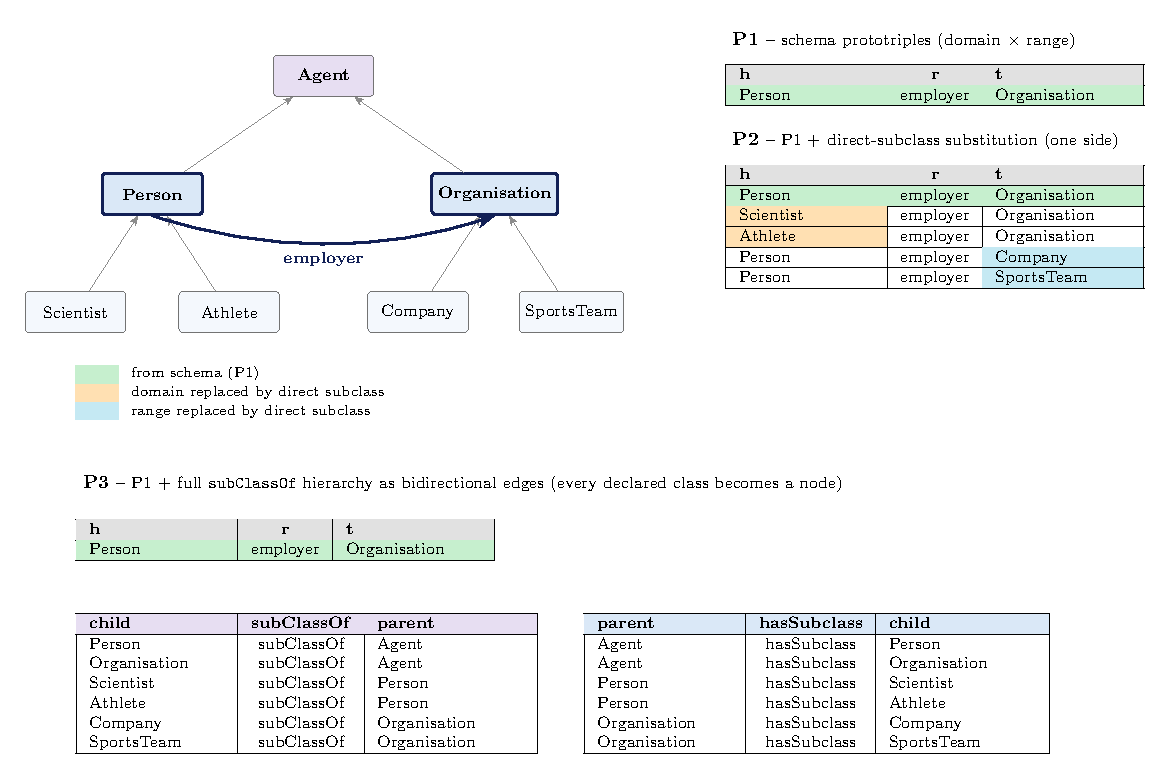
\includegraphics[width=\linewidth]{assets/protograph_construction.pdf}
  \caption[Construction of protographs P1, P2 and P3]{%
    Construction of the three protographs from a small DBpedia schema excerpt
    (declared classes only; no \texttt{owl:Thing}, so no universal-root hub).
    \textbf{P1} emits one prototriple per relation from its declared domain and
    range, here $(\mathit{Person}, \mathit{employer}, \mathit{Organisation})$.
    \textbf{P2} adds one-sided direct-subclass substitutions of the domain
    (orange) or range (blue) class. \textbf{P3} (introduced in
    Section~\ref{sec:p3}) instead extends P1 with the full \texttt{subClassOf}
    hierarchy as explicit bidirectional edges
    (\texttt{subClassOf}/\texttt{hasSubclass}), so every declared class becomes a
    protograph node. P1 is contained in both P2 and P3, while P2 and P3 are
    independent expansions of P1.}
  \label{fig:protograph_construction}
\end{figure}

\paragraph{Protograph pre-training.} We generate random walks over the
protograph and train a skip-gram model on them, yielding a pretrained
embedding for every class and relation token that occurs in the
protograph.

\paragraph{Transfer.} The fine-tuning model is a fresh skip-gram (word2vec)
model over the instance-graph walks, trained exactly as in a standard RDF2Vec
run; the \emph{only} difference is where its vectors start. Instead of
gensim's~\cite{rehurek_software_2010} random initialization, we seed the model
with the pretrained protograph
embeddings, so that schema knowledge takes the place of random vectors. In
detail, we build the fine-tuning vocabulary from the instance-graph walks and
then apply two rules: (i) every token that also exists in the protograph vocabulary
(this concerns \emph{both classes and relations}) receives its pretrained
vector directly; (ii) every typed instance entity is
initialized from the embeddings of its classes according to an initialization
strategy (Section~\ref{sec:init_strategies}). Tokens covered by neither rule
keep gensim's random initialization. The transferred vectors are written to
both RDF2Vec matrices (input vectors and \texttt{syn1neg}); we examine this choice
in Section~\ref{sec:norm}.

\paragraph{Fine-tuning.} From this initialization, training proceeds with
ordinary skip-gram on the instance-graph walks: the protograph vectors are
simply the initial weights and are updated by the usual gradients, with no token
frozen. Entity embeddings are evaluated with the DLCC logistic-regression
protocol after every epoch.

\subsection{Extended Protographs: P3}
\label{sec:p3}

P1 and P2 leave many leaf classes without pretrained embeddings
(Section~\ref{sec:coverage}), and the obvious remedy of climbing the hierarchy
at initialization time (\texttt{all\_init}, Section~\ref{sec:init_strategies})
reaches full coverage only by copying an ancestor's vector onto every uncovered
leaf, which collapses distinct leaves onto a shared embedding. We therefore add
a third protograph, \textbf{P3}, which extends P1 with the \emph{full}
\texttt{subClassOf} hierarchy, encoded as explicit bidirectional edges
(\texttt{subClassOf}/\texttt{hasSubclass}) between class tokens. P3 has two
advantages. First, coverage: every class reachable in the hierarchy becomes a
protograph node and therefore obtains a pretrained embedding, so every typed
instance can be initialized without falling back to random vectors. Second, and
unlike the climbing strategies, the hierarchy itself becomes part of the
pre-training corpus: the random walks now traverse \texttt{subClassOf} edges
freely, exploring the whole ontology rather than only the isolated
domain/range prototriples of P1 and P2. Each class (including every
leaf) thus receives its \emph{own} embedding, shaped by its position in the
hierarchy through co-occurrence with its super- and subclasses, instead of a
copy of an ancestor's vector. The class hierarchy is in this way learned
distributionally rather than imposed at initialization time. P3 is also
available to the classic transfer, a baseline we denote \texttt{p3\_classic} and
evaluate in Section~\ref{sec:results_synthetic}.

\subsection{Initialization Coverage}
\label{sec:coverage_concept}

P1, P2, and P3 differ in how much schema information enters the protograph: P1
uses relation domain and range declarations, P2 additionally adds direct
subclass edges, and P3 adds the full subclass hierarchy. A natural question is
whether this extra pretraining signal actually reaches the entities that matter
for DLCC classification. We therefore track \emph{initialization coverage}: how
many vocabulary tokens and classification entities start fine-tuning with a
protograph-derived embedding instead of a random Word2Vec initialization.

We distinguish two levels of coverage. At the \textbf{vocabulary} level, we
count all tokens in the fine-tuning Word2Vec vocabulary: how many were
initialized from protograph pretraining, how many of
those are entity vs.\ relation tokens, and how many remained at random
initialization. At the \textbf{training-set} level, we apply the same
split to the 1600 training entities (800 positive, 800 negative) that DLCC
provides for the classifier. The measured coverage for P1, P2, and P3, and its
relationship to final accuracy, are reported in Section~\ref{sec:coverage}.

\section{Initialization Strategies along the Class Hierarchy}
\label{sec:init_strategies}

The MASCHInE rule initializes an instance with the mean of the embeddings of its
\emph{most specific} classes. On the DLCC ontologies this rule frequently
fails: instances are typed with deep leaf classes, while the P1 protograph
contains only classes that appear in domain/range declarations, and P2 only
adds their direct subclasses. A leaf class therefore often has no pretrained
embedding at all, and the instance falls back to random initialization. We
implemented and compared four strategies:

\begin{description}
  \item[\texttt{most\_specific}] the MASCHInE rule: mean of the embeddings of the
    instance's most specific classes; instances whose classes are all
    out-of-vocabulary stay random.
  \item[\texttt{all\_init}] like \texttt{most\_specific}, but when a class has
    no pretrained embedding, we climb the \texttt{subClassOf} hierarchy upward until
    an ancestor with an embedding is found and use that ancestor's embedding instead.
    This guarantees an initialization for every instance whose class hierarchy
    reaches a covered class.
  \item[\texttt{average\_hier}] mean over the embeddings of the instance's classes
    \emph{and all their transitive superclasses}, mixing specific and general
    signal uniformly.
  \item[\texttt{weight\_hierarchy}] like \texttt{average\_hier}, but ancestors
    at hop distance $d$ above the most specific classes are down-weighted by a
    decay factor $\lambda^d$ (default $\lambda = 0.5$), so that specific
    classes dominate and general classes contribute residually.
\end{description}

\begin{figure}[tbp]
  \centering
  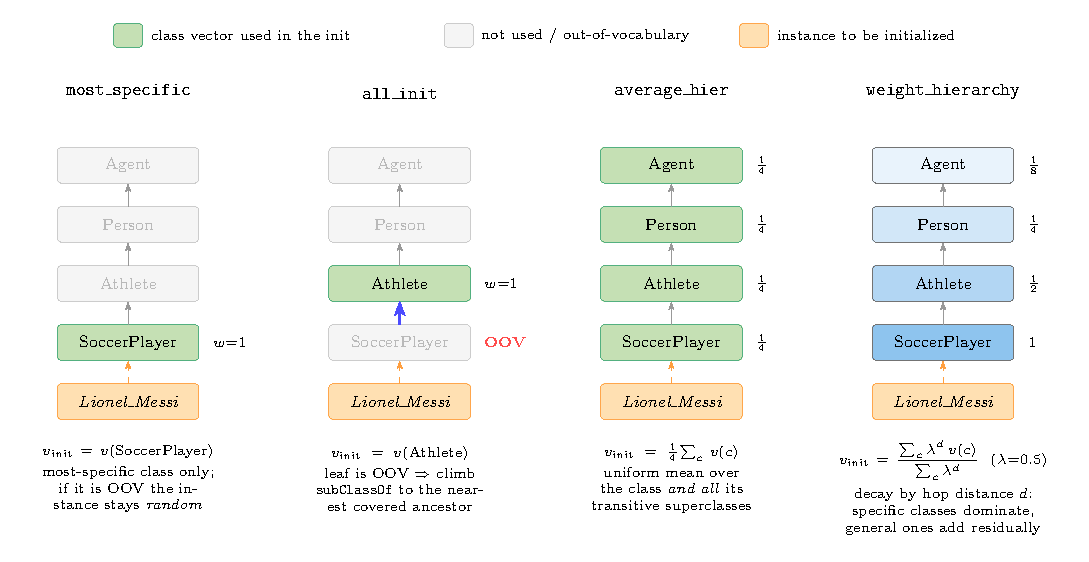
\includegraphics[width=\linewidth]{assets/init_strategies_diagram.pdf}
  \caption[Class-based initialization strategies]{%
    The four initialization strategies for an instance
    (\texttt{dbr:Lionel\_Messi}, typed \texttt{SoccerPlayer} $\sqsubseteq$
    \texttt{Athlete} $\sqsubseteq$ \texttt{Person} $\sqsubseteq$ \texttt{Agent}).
    Green class boxes contribute their pretrained vector to the initialization,
    with the weight shown on the right. \texttt{all\_init} is drawn for the case
    where the most-specific class is out-of-vocabulary, the only case in which it
    differs from \texttt{most\_specific}.}
  \label{fig:init_strategies}
\end{figure}

Figure~\ref{fig:init_strategies} contrasts the four strategies on a single
worked example. The motivation for these strategies was purely the coverage problem of the
classic transfer: \texttt{all\_init} was our first remedy for instances whose
most specific class has no pretrained embedding: instead of leaving such an
instance at random initialization, we walk up its class hierarchy until we
reach a class that is in the pretraining vocabulary and initialize from that
ancestor's embedding. \texttt{average\_hier} and \texttt{weight\_hierarchy}
generalize the same idea by blending the whole ancestor closure into the
initialization. All four strategies remain within the classic transfer
paradigm; they change \emph{which} class vectors seed an instance, not
\emph{what} the initialization encodes (this distinction becomes central in
Section~\ref{sec:method_overview}). Unless stated otherwise, our experiments
use \texttt{most\_specific} for comparability with MASCHInE.

A dedicated head-to-head comparison of the four strategies (varying \emph{only}
which class vectors seed an instance) is reported in
Section~\ref{sec:results_init_strategies}. Anticipating that result: the three
climbing strategies reach full initialization coverage but \emph{none} improves
final accuracy over \texttt{most\_specific}. One possible explanation is that
filling coverage by sharing ancestor vectors over-smooths the embeddings. Either way, the comparison already signals
the central lesson of this chapter, namely that \emph{what} the initialization
encodes matters more than how many entities it covers, which we now make precise.

\subsection{Limitations of the Classic Transfer}
\label{sec:classic_limits}

Before turning to the proposed method, we ask whether the classic transfer can
simply be tuned into a stronger baseline. We test this with three controlled
ablations. Each keeps the classic initialization rule intact and changes only
the training around it. The first lowers the fine-tuning learning rate, so the
transferred vectors move less (Section~\ref{sec:abl_lr}, with results in
Section~\ref{sec:results_lr}). The second anchors the embeddings back toward
their schema-informed initialization during fine-tuning
(Section~\ref{sec:anchoring}, with results in Section~\ref{sec:results_anchoring}).
The third adds small Gaussian noise, so co-initialized instances start from
slightly different positions (Section~\ref{sec:jitter}, with results in
Section~\ref{sec:results_jitter}). None of the three gives a reliable gain over
the from-scratch \texttt{vanilla} baseline. A low learning rate only
\emph{freezes} the coarse classic initialization in place and collapses P1.
Anchoring is at best inert at small strength, and pushes every transfer below
\texttt{vanilla} once it is strong enough to matter. The noise hurts any variant
that carries signal, and does nothing where the classic transfer already sits
near chance. The classic transfer therefore helps only where the label \emph{is}
the instance's own class. On tc14, for example, it reaches accuracy~1.00 already
at initialization. Everywhere else it is largely inert, no matter how the
surrounding training is configured.

The reasons are structural rather than a matter of tuning. Four of them explain
the behaviour, and each points to a concrete repair that the concept-bound
initialization of Section~\ref{sec:method_overview} implements.

\begin{enumerate}
  \item \textbf{Own-class initialization carries no signal for
    relation-centric tasks.} On tc07--tc12, all labeled entities share the
    same class; initializing an entity from \emph{its own} class therefore
    produces (near-)identical vectors for positives and negatives. The
    decision-relevant information sits instead in the entity's \emph{edges} --
    the classes of its \emph{neighbours} on the typed tasks (tc07, tc08, tc11,
    tc12) and the edge \emph{count} on the type-agnostic cardinality tasks (tc09,
    tc10, cf.\ failure mode~4) -- which the initialization rule never explicitly
    touches.
  \item \textbf{Skip-gram summation destroys relation--class binding.} Even
    if neighbour-class information reached the embedding, an RDF2Vec embedding is
    a bag of context vectors: ``has $r$ to a $C$-thing'' becomes
    indistinguishable from ``has $r$ to a $C'$-thing and some other edge to a
    $C$-thing''. The DLCC concepts $\exists r.C$ are defined over
    (relation, class) \emph{pairs}, and plain summation erases the pairing.
  \item \textbf{Coverage gaps.} Instances are typed with deep leaf classes
    that P1, and to a lesser degree P2, do not contain
    (Section~\ref{sec:coverage}); those instances start from random vectors.
    The \texttt{all\_init} strategy and the hierarchy-covering P3 protograph
    (Section~\ref{sec:p3}) are needed to close this gap.
  \item \textbf{Magnitude information is fragile.} The cardinality tasks
    tc09--tc12 require counting edges, a signal that can only survive in the
    \emph{norm} of an embedding. Per-vector normalization, standard in the
    MASCHInE pipeline, erases it, and unprotected fine-tuning randomizes
    it.
\end{enumerate}


\section{Concept-Bound Protograph Initialization}
\label{ch:method}
\label{sec:concept_bound}

\begin{figure}[t]
  \centering
  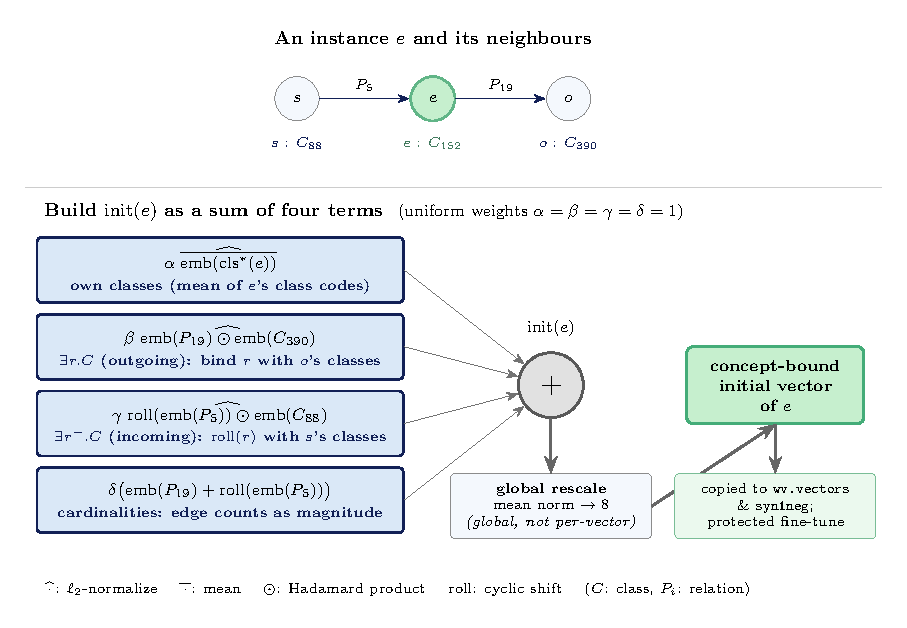
\includegraphics[width=\linewidth]{assets/bound_init_construction_simple.pdf}
  \caption{Concept-bound construction of the initial vector $\mathrm{init}(e)$ of
  an instance $e$ (Equation~\eqref{eq:bound_init}). Each of the four terms is
  assembled from the pretrained, unit-normalized protograph codes of the classes
  and relations in $e$'s instance-graph neighbourhood; the terms are summed and
  rescaled to the shared target norm, then copied into both RDF2Vec matrices for
  protected fine-tuning.}
  \label{fig:bound_init_construction}
\end{figure}

This section introduces our proposed method. Its key idea is to reinterpret the
pretrained protograph vectors: rather than viewing them as \emph{initial values
to be improved by fine-tuning}, we treat them as \emph{symbols} and use them to
construct, for every instance, an explicit superposition of the one-hop schema
concepts that the instance satisfies. The classic transfer hopes that
fine-tuning will, on its own, combine own-class vectors into neighbour-aware
features. We instead compute those features directly at initialization time,
encoding relation--class \emph{bindings} and edge \emph{counts} explicitly, and
then protect them during fine-tuning. We describe
the components in the order in which they were developed: notation and the
overall construction (Section~\ref{sec:method_overview}), normalization and
protected fine-tuning (Section~\ref{sec:norm}), Hadamard binding of relations
and neighbour classes (Section~\ref{sec:binding}), and direction-aware
cardinality encoding (Section~\ref{sec:cardinality}). The construction reuses
the protographs of Section~\ref{sec:protograph_construction};
Section~\ref{sec:method_summary} assembles the full recipe.
Figure~\ref{fig:bound_init_construction} gives a schematic overview of the whole
construction.

\subsection{Overview and Notation}
\label{sec:method_overview}

We first fix the notation. Let $\mathrm{emb}(x) \in \mathbb{R}^d$ be the
pretrained protograph embedding of a class or relation token $x$, normalized as
described below, and let $\mathrm{cls}^*(e)$ be the set of \emph{materialized}
classes of an entity $e$, that is, its asserted classes together with all of
their transitive superclasses. This materialization step is important, because
the classes that discriminate the DLCC tasks are often superclasses of the
asserted leaf types; projecting every instance onto its full ancestor set is
therefore what makes the class signal linearly accessible. Finally, we write
$\odot$ for the element-wise (Hadamard) product, $\mathrm{roll}(\cdot)$ for a
circular shift of a vector by one dimension, and $\widehat{v} = v / \lVert v
\rVert$ for $\ell_2$ normalization.

The concept-bound initialization of an instance $e$ is
\begin{equation}
\label{eq:bound_init}
\begin{aligned}
\mathrm{init}(e)
={}& \underbrace{\alpha \;\widehat{\textstyle\frac{1}{|\mathrm{cls}^*(e)|}\sum_{C \in \mathrm{cls}^*(e)} \mathrm{emb}(C)}}_{\text{own classes}} \\
&+ \underbrace{\beta \sum_{(e,r,o)} \sum_{C \in \mathrm{cls}^*(o)} \widehat{\mathrm{emb}(r) \odot \mathrm{emb}(C)}}_{\exists r.C \text{ (outgoing)}} \\
&+ \underbrace{\gamma \sum_{(s,r,e)} \sum_{C \in \mathrm{cls}^*(s)} \widehat{\mathrm{roll}(\mathrm{emb}(r)) \odot \mathrm{emb}(C)}}_{\exists r^{-}.C \text{ (incoming)}} \\
&+ \underbrace{\delta \Big( \sum_{(e,r,\cdot)} \mathrm{emb}(r) + \sum_{(\cdot,r,e)} \mathrm{roll}(\mathrm{emb}(r)) \Big)}_{\text{cardinalities}}
\end{aligned}
\end{equation}
with uniform coefficients $\alpha = \beta = \gamma = \delta = 1$ throughout
this thesis. The terms target the failure modes of
Section~\ref{sec:classic_limits}, with one repair handled outside the equation.
The $\alpha$-term carries over the classic own-class signal as a base; the
$\beta$- and $\gamma$-terms supply the neighbour-class information missing in
failure mode~1 while restoring the relation--class binding of failure mode~2, in
both edge directions; and the $\delta$-term accumulates plain relation embeddings
so that the edge counts of failure mode~4 survive as vector magnitude. The
remaining coverage gap (failure mode~3) is closed not by a term but by the
\texttt{all\_init}/P3 fallback described next. We keep the
coefficients uniform deliberately, to isolate the contribution of each term.
Instances not
covered by Equation~\eqref{eq:bound_init} (e.g.\ isolated nodes) fall back to
the classic class-mean rule with the \texttt{all\_init} hierarchy-climbing
strategy of Section~\ref{sec:init_strategies}.

\subsection{Normalization and Protected Fine-Tuning}
\label{sec:norm}

Two normalization decisions and a protected fine-tuning regime turn out to be
preconditions for everything else; without them, the more elaborate terms of
Equation~\eqref{eq:bound_init} have no measurable effect.
Figure~\ref{fig:norm_pipeline} summarizes the resulting pipeline, from the
pretrained codes to the protected fine-tune.

\begin{figure}[htbp]
  \centering
  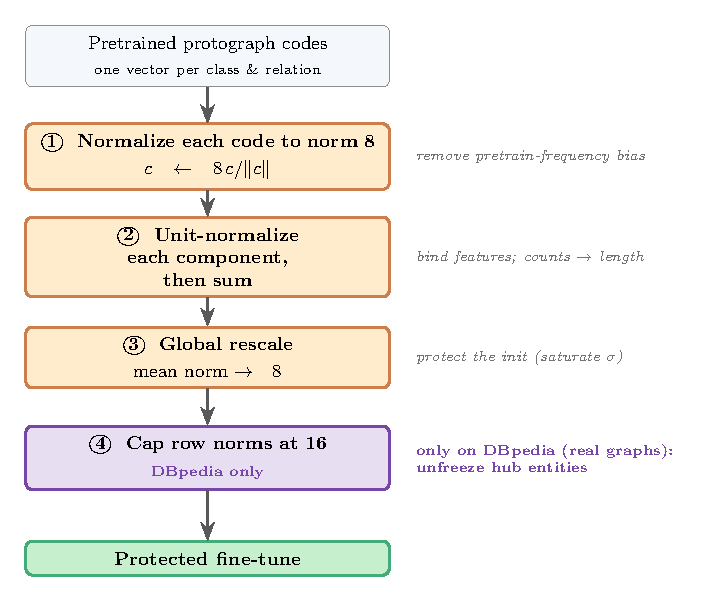
\includegraphics[width=0.72\linewidth]{assets/normalization_pipeline.pdf}
  \caption[Normalization pipeline of the concept-bound initialization]{%
    Normalization pipeline of the concept-bound initialization. Pretrained codes
    are scaled to a common norm~(\textcircled{1}); each component of
    Equation~\eqref{eq:bound_init} is unit-normalized before summation, so that
    repeated edges accumulate magnitude and encode counts~(\textcircled{2}); the
    assembled instance vectors are then rescaled by a \emph{single} shared scalar
    to mean norm~$8$~(\textcircled{3}). On DBpedia only, an additional per-row cap
    at~$16$ clamps the heavy-tailed hub norms~(\textcircled{4}). The protected
    fine-tune adapts the initialization without eroding it. The classic transfer
    of Section~\ref{sec:init_strategies} shares step~\textcircled{1} and the
    fine-tune, but replaces steps \textcircled{2}--\textcircled{3} with a
    per-vector renormalization of each instance vector to norm~$8$.}
  \label{fig:norm_pipeline}
\end{figure}

\paragraph{Unit-normalize codes and components.} Raw pretrained vectors carry
strong frequency artifacts: tokens that occur often in protograph walks acquire
larger norms. Because the embeddings enter Equation~\eqref{eq:bound_init} as
\emph{symbols}, not as quality-weighted estimates, we $\ell_2$-normalize every
code (each class and relation embedding) to unit length before use, so that a
frequent class and a rare class contribute on equal footing. As a result every
\emph{component} that enters the sum is itself a unit vector. The own-class mean
and each bound $(r, C)$ pair come out non-unit from the averaging and the
Hadamard product, so they are explicitly renormalized to unit length, which is
what the hats $\widehat{(\cdot)}$ in Equation~\eqref{eq:bound_init} denote; the
bare relation codes of the cardinality $\delta$-term are already unit and so
enter directly, without an extra hat. No per-entity sum is renormalized, which is
exactly why repeated edges accumulate magnitude and encode counts
(Section~\ref{sec:cardinality}). The classic transfer of
Section~\ref{sec:init_strategies}, by contrast, uses the same codes but scaled
directly to norm $8$ and consumed without this per-component step.

\paragraph{Shared target norm.} Once a vector has been assembled for every
instance, the entire set is rescaled by a \emph{single} shared scalar so that the
\emph{mean} instance norm equals a target value (\texttt{TARGET\_NORM} $= 8$ in
all experiments). Two properties matter. First, the rescaling is \emph{global}
(one scalar for the whole matrix) and never per-vector: a per-vector
normalization would place every instance on a sphere of radius $8$ and erase
exactly the magnitude differences that the $\delta$-term creates to encode
cardinalities. Second, large shared norms saturate the RDF2Vec sigmoid, so
gradients on well-aligned (vector, context) pairs become small, which slows the
erosion of the transferred structure during fine-tuning.

\paragraph{Mirroring into the context matrix.} The initialization is written
to \emph{both} RDF2Vec matrices: the input vectors and the negative-sampling
output matrix \texttt{syn1neg}. This mirroring is not specific to the
concept-bound construction; it is the shared MASCHInE-style transfer applied to
the classic variants as well (Section~\ref{sec:p1p2}), and what distinguishes
the concept-bound init is the per-component normalization and global rescaling
above, not where the vectors are written. If only the input vectors were set, the random
context matrix would immediately pull them toward arbitrary directions; with
mirrored matrices, the first epochs of fine-tuning reinforce rather than
destroy the transferred geometry.

\paragraph{Protected learning rate.} Fine-tuning uses a learning rate of
0.0025, one tenth of the from-scratch default. Combined with the saturated
sigmoid, this keeps per-epoch accuracy curves nearly flat on tasks the
initialization already solves, while still allowing instance-specific
adaptation. The from-scratch rate of 0.025, by contrast, visibly erodes the
initialization within one to two epochs
(cf.\ Section~\ref{sec:forgetting}).

\subsection{Binding Relations and Neighbour Classes}
\label{sec:binding}

The $\beta$- and $\gamma$-terms of Equation~\eqref{eq:bound_init} target the
binding problem of Section~\ref{sec:classic_limits}, where a sum of separate
relation and class vectors cannot record which relation points to which class.
To recover that link we borrow the binding operation from vector-symbolic
architectures. The Hadamard product $\mathrm{emb}(r) \odot \mathrm{emb}(C)$ of
two (approximately) random unit vectors is approximately orthogonal both to its
own factors and to the product of any other (relation, class) pair. A sum of
such bound pairs therefore behaves like a \emph{readable set} of $(r, C)$
features: a linear classifier can test whether a specific pair is present
without interference from the entity's other edges. This is exactly the form
taken by the qualified-existential DLCC concepts $\exists r.C$ (tc07) and
$\exists r^{-}.C$ (tc08), and the same $(r, C)$ pairing underlies the
qualified-cardinality tasks $\geq 2r.T$ (tc11) and $\geq 2r^{-1}.T$ (tc12).

The two terms differ only in how they treat edge direction. For incoming edges
the relation embedding is tagged with a circular shift ($\mathrm{roll}$) before
binding, so that $\exists r.C$ and $\exists r^{-}.C$ occupy distinguishable
subspaces. In both cases each bound pair is normalized to unit length before it
is accumulated, so that a single entity's feature set is an unweighted sum of
unit features. Repeated (relation, class) pairs then add magnitude rather than
new directions, which is the intended behaviour and is exploited by the
cardinality term of the next section.

\subsection{Direction-Aware Cardinality Encoding}
\label{sec:cardinality}

The $\delta$-term encodes \emph{how many} edges of each relation an entity has.
Each outgoing $r$-edge adds $\mathrm{emb}(r)$, so two such edges add the vector
twice, and the count survives as magnitude along the $\mathrm{emb}(r)$
direction. This magnitude is readable by a linear probe and is preserved by the
global (rather than per-vector) rescaling of Section~\ref{sec:norm}.

The treatment of edge \emph{direction} is a subtle design choice. A
direction-blind count term, in which an incoming $r$-edge adds the same
$\mathrm{emb}(r)$ as an outgoing one, aliases distinct degree profiles: an
entity with two outgoing $r$-edges would be indistinguishable, in the count
channel, from one with one outgoing and one incoming $r$-edge. We therefore tag
incoming edges with $\mathrm{roll}(\mathrm{emb}(r))$, reusing the fixed
permutation already applied in the $\gamma$-term. A circular shift of a
high-dimensional random unit vector is nearly orthogonal to the original
(empirically, mean cosine $\approx -0.04$ over the pretrained relation
embeddings), so outgoing and incoming counts occupy quasi-independent channels
that a linear classifier can read out separately.

We regard the direction tag as a genuine design choice rather than an
implementation detail, and we ablate it in Section~\ref{sec:abl_direction},
comparing the default \texttt{rolled} tag against direction-blind, negated, and
keyed alternatives.

\subsection{Summary of the Method}
\label{sec:method_summary}

Putting the pieces together, the complete pipeline proceeds in four steps:

\begin{enumerate}
  \item \textbf{Pretrain} skip-gram embeddings on random walks over a
    protograph (P1, P2, or the hierarchy-covering P3) to obtain one embedding
    per class and relation.
  \item \textbf{Normalize} every embedding to unit length.
  \item \textbf{Construct} the concept-bound initialization of each instance
    through Equation~\eqref{eq:bound_init}, using the rolled direction tag and
    the uniform coefficients $\alpha = \beta = \gamma = \delta = 1$. Every
    component is a unit vector (the own-class mean, every bound $(r, C)$ pair,
    and every bare relation code alike), so edge counts are encoded by
    accumulation alone: the same unit code is added once per incident edge, and
    no per-entity sum is renormalized. The assembled vectors are then rescaled
    globally to the shared target norm and mirrored into both RDF2Vec matrices.
  \item \textbf{Fine-tune} on instance walks at the protected learning rate
    ($0.0025$) with no initialization noise, evaluating after every epoch.
\end{enumerate}

Conceptually, protograph pretraining supplies a vocabulary of quasi-orthogonal
symbols, and the concept-bound construction assembles those symbols into a
one-hop schema feature vector for each entity. Fine-tuning then only has to add
instance-specific information on top of features that the DLCC classifier can
already read, rather than discovering those features from scratch through walk
co-occurrence.

\section{Ablation Studies}
\label{sec:ablations}

Beyond the components of the proposed method, we study a set of design choices
through controlled ablations. Each ablation isolates a single knob, namely the
fine-tuning learning rate, protograph anchoring, initialization noise, the walk
budget, or the direction tag of the cardinality term, while holding the rest
of the pipeline fixed. Beyond confirming that each knob behaves as the
construction predicts, the ablations share a common motivation: taken together
they attribute the concept-bound gains to identifiable mechanisms rather than to
luck, and in particular they rule out the simplest rival explanation, that the
construction merely acts as a generic regularizer. This section states what each
ablation varies and why; the corresponding empirical results are reported in
Chapter~\ref{ch:experiments}.

\subsection{Fine-Tuning Learning Rate}
\label{sec:abl_lr}

A lower fine-tuning learning rate is motivated by two questions. The first
concerns the classic transfer. The schema-informed vectors drift far during
fine-tuning: the embedding drift $1 - |\cos(\mathbf{v}_0, \mathbf{v}_t)|$, averaged
across entities, rises sharply within the first one to two epochs
(Section~\ref{sec:results_drift}). A natural hypothesis is therefore that the
transfer fails to improve over \texttt{vanilla} not because the initialization
lacks signal, but because whatever signal it carries is overwritten before the
model is saved. If that were the cause, perturbing the transferred vectors less
should let the preserved signal survive and lift the classic transfer above
\texttt{vanilla}. The second question concerns the concept-bound method, for
which the same low rate is one of the preconditions the construction relies on:
we ask whether the low rate is a free lunch, that is, a generally safe choice
that any variant can adopt, or a precondition specific to the bound construction.

We experiment with reducing the learning rate during fine-tuning. Since the
protograph-initialized models start from schema-trained embeddings rather than
random vectors, the goal of fine-tuning is not to learn the embedding space from
scratch, but to adapt the schema-informed space to the instance graph. A smaller
learning rate therefore acts as a conservative fine-tuning strategy: it limits
abrupt changes to the transferred embeddings and may reduce the overwriting of
schema-level information. However, if the learning rate is chosen too small, the
model may underfit the instance graph because the embeddings cannot move
sufficiently from their initial positions.

The results (Section~\ref{sec:results_lr}) show that lowering the rate helps no
classic transfer: it leaves \texttt{p2\_classic} essentially unchanged
($0.765 \rightarrow 0.759$), modestly hurts \texttt{p3\_classic}
($0.774 \rightarrow 0.741$), and collapses \texttt{p1\_classic}
($0.758 \rightarrow 0.609$). The protected low rate is thus a property the
concept-bound construction \emph{requires} rather than a generally safe choice,
so the classic variants are fine-tuned at the from-scratch rate $0.025$
throughout.

\subsection{Protograph Anchoring}
\label{sec:anchoring}

The embedding-drift analysis (Section~\ref{sec:results_drift}) shows that
fine-tuning overwrites much of the transferred schema signal. Anchoring is an
attempt to treat that overwriting directly: by pulling each instance back toward
its schema-informed initialization during fine-tuning, it forces the schema
signal to be retained. If overwriting is what holds the classic transfer back,
retaining the signal this way should let the classic transfer improve over
\texttt{vanilla}.

The ablation also serves a second purpose. A reader might object that the
concept-bound construction helps only because any structured constraint on the
embeddings acts as a regularizer, independently of the schema content it encodes.
Anchoring is exactly such a generic constraint, as is the Gaussian noise of the
ablation in Section~\ref{sec:jitter}: anchoring pulls the vectors toward a fixed
point, and noise perturbs them, and neither adds schema information. If generic
regularization were the source of the gains, adding either should help. Showing
instead that both are inert at best, and harmful once strong, leaves the encoded
schema features as the remaining explanation for the gains.

To preserve schema-level information during instance-level RDF2Vec training, we
introduce an anchoring regularization term. After protograph pretraining, each
instance embedding is initialized with the embedding of its corresponding class.
During fine-tuning, the anchoring term penalizes deviations from this initial
schema-informed vector:
\[
\mathcal{L}_{total}
=
\mathcal{L}_{RDF2Vec}
+
\lambda
\sum_{e \in E_{anchored}}
\lVert \mathbf{v}_e - \mathbf{v}^{0}_e \rVert_2^2 .
\]
Here, \(\mathbf{v}_e\) denotes the current instance embedding, \(\mathbf{v}^{0}_e\) denotes the transferred protograph-based initialization, and \(\lambda\) controls the strength of the regularization.
A small value of \(\lambda\) allows the entity embeddings to adapt to the instance graph while discouraging complete overwriting of the schema information learned during protograph pretraining.

In practice we realize the penalty as its closed-form proximal step rather than
adding an explicit term to the RDF2Vec objective: at the end of every fine-tune
epoch \emph{including the last}, each anchored instance is pulled a fraction
\(\lambda\) of the way back toward its initialization,
\(\mathbf{v}_e \leftarrow (1-\lambda)\,\mathbf{v}_e + \lambda\,\mathbf{v}^0_e\).
Because the final epoch is anchored as well, the saved model's anchored instances
are pulled back toward their schema-informed initialization before being frozen.
\(\lambda=0\) recovers the plain protograph transfer; \(\lambda=1\) hard-resets
the anchored instances to their class initialization after every epoch, the last
included, so the saved anchored vectors equal their class initialization exactly.
The anchored set \(E_{anchored}\) is exactly the instances that
received a class-based initialization (\texttt{most\_specific} rule); copied
protograph rows and randomly-initialized instances are left free.

The results (Section~\ref{sec:results_anchoring}) show no reliable benefit:
small \(\lambda\) is essentially inert, while strong \(\lambda\) drives every
transfer well below \texttt{vanilla} (down to \(0.564\) at \(\lambda=1\)), with a
genuine, sustained improvement on only one test case (tc14, whose
class-membership label is already encoded by the initialization). We therefore
set \(\lambda=0\) (no anchoring) in all other experiments.

\subsection{Random Initialization Noise}
\label{sec:classic_noise}
\label{sec:jitter}

We also add small Gaussian noise to the initialized embeddings of both the
classic and the concept-bound variants. The first motivation comes from the
classic transfer. The \texttt{most\_specific} rule seeds every instance of a
class from that single class code (Section~\ref{sec:classic_limits}), so many
instances are mapped to the same starting vector. When all of these instances
begin from exactly the same point, the model has no entity-specific variation to
work from. We therefore perturb every initialized entity \(e\) as
\[
\mathbf{v}_e^{0}
=
\mathrm{init}(e)
+
\epsilon_e,
\qquad
\epsilon_e \sim \mathcal{N}(0, \sigma^2),
\]
where \(\mathrm{init}(e)\) is the entity's initialization. For the classic
variants this is the \texttt{most\_specific} class code; for the bound variants
it is the concept-bound construction of Equation~\eqref{eq:bound_init}. The
perturbation is kept small, so the embedding stays close to its schema-informed
starting point while different instances still occupy slightly different
positions.

Under the concept-bound initialization this first motivation largely disappears,
because entities with different neighbourhoods already receive different vectors
by construction. Noise could nonetheless act as a generic regularizer, and this
gives the ablation its second motivation: it checks whether the concept-bound
gains are merely a regularization effect rather than a product of the schema
content the construction encodes. We therefore run a factorial ablation. The
noise scale $\sigma \in \{0, 0.05, 0.1, 0.2, 0.5\}$ is added to the initialized
vectors (after norm scaling) and crossed with all protographs (P1/P2/P3), both
initialization schemes (classic, bound), and the direction tag (on/off). The
results (Section~\ref{sec:results_jitter}) are uniform: $\sigma=0$ is best for
every variant that carries signal. Noise degrades the concept-bound
initialization smoothly and leaves the near-chance classic variants unchanged.
As a regularizer it is therefore strictly harmful, and it is never enabled.

\subsection{Reducing Fine-Tuning Walks}
\label{sec:nw50}

Two observations motivate this ablation. First, the protograph-initialized
variants start fine-tuning from a lower training loss than \texttt{vanilla}.
Second, for the concept-bound variants the accuracy already present at
initialization (epoch 0) is close to the final accuracy, and the diagnostics show
that further fine-tuning mostly erodes the bound features rather than adding
signal (Section~\ref{sec:results_diagnostics}, Section~\ref{sec:results_drift}).
Together they raise a practical question: can the schema-informed initialization
\emph{buy} fine-tuning budget? Walk generation and RDF2Vec training both scale
linearly with the number of walks, so the walk budget is the main cost lever of
the whole pipeline. To answer the question we compare
\emph{unequal} budgets: \texttt{vanilla} on the full instance-walk corpus
(100 walks per entity, the comparison configuration of
Section~\ref{sec:setup}) against the schema-informed variants on a half (50) and
a quarter (25) of it, with a reduced-corpus \texttt{vanilla} run as a control.
The results (Section~\ref{sec:nw_revisited}) split by variant: the classic
transfer only \emph{matches} full-budget \texttt{vanilla} at half budget,
whereas the concept-bound variants are insensitive to the cut and even improve
as it shrinks. At a quarter of the corpus \texttt{p2\_bound} beats full-budget
\texttt{vanilla} by roughly $30$ points on the relation-centric focus set while
spending about $3.6\times$ less time in fine-tuning.

\subsection{Direction-Aware Cardinality}
\label{sec:abl_direction}

To establish that the direction tag of the cardinality term
(Section~\ref{sec:cardinality}) is a real design dimension and not an
implementation detail, we ablate four direction tags for the incoming-edge
embedding: \texttt{shared} (direction-blind, $\mathrm{emb}(r)$), \texttt{rolled}
($\mathrm{roll}(\mathrm{emb}(r))$, the default), \texttt{negated}
($-\mathrm{emb}(r)$, which encodes $\text{out} - \text{in}$ in a single
channel), and \texttt{keyed} ($\mathrm{emb}(r) \odot k$ for a fixed random
$\pm 1$ key $k$, an alternative decorrelating tag). The hypotheses: direction is
label-relevant information on the inverse-direction DLCC tasks, any fixed
decorrelating norm-preserving tag recovers it, and negation is a tag that loses
information differently. The results (Section~\ref{sec:results_direction})
confirm all three: a direction-blind count term adds nothing over the count-free
baseline ($0.838$ vs.\ $0.845$ mean), the default \texttt{rolled} tag lifts the
mean to $0.912$, the random \texttt{keyed} tag performs on par ($0.903$), and
\texttt{negated} fails back at the direction-blind level ($0.832$).

%=====================================================================
\chapter{Experimental Evaluation}
\label{ch:experiments}
\label{ch:results}

This chapter evaluates the proposed method. We first describe the experimental
setup (Section~\ref{sec:setup}) and compare all variants on the synthetic DLCC
test cases (Section~\ref{sec:results_synthetic}). We then report the runtime
overhead of schema-based pretraining (Section~\ref{sec:results_runtime}) and
quantify how much of the vocabulary each initialization covers, showing that
broader coverage does not by itself raise accuracy
(Section~\ref{sec:coverage}). We inspect the embedding spaces to explain
\emph{why} the concept-bound initialization succeeds where the classic transfer
fails (Section~\ref{sec:results_diagnostics}). A series of ablations then isolates
the contribution of each design choice (Section~\ref{sec:results_ablations}). We
close by validating the findings on the DBpedia DLCC gold standard
(Section~\ref{sec:results_dbpedia}) and on standard downstream tasks
(Section~\ref{sec:dbpedia_geval}).

\section{Experimental Setup}
\label{sec:setup}

\paragraph{Datasets.} The synthetic experiments use the DLCC synthetic gold
standard test cases tc01--tc12 \cite{portisch_dlcc_2022} and our three
additional schema-specific test cases tc13--tc15
(Section~\ref{sec:new_tcs}), each with 1\,000 positive and 1\,000 negative
labeled entities and fixed train/test splits. The DBpedia experiments use the
DLCC DBpedia gold standard (tc01--tc12 instantiated over six domains, size
bucket 5\,000, regular and hard splits; 89 splits in total) over a DBpedia
subgraph materialized with type and hierarchy information.

\paragraph{Variants.} We compare: \texttt{vanilla} (random initialization,
from-scratch training); \texttt{p1\_classic}, \texttt{p2\_classic},
\texttt{p3\_classic} (protograph pretraining with \texttt{most\_specific} class
initialization, fine-tuned at the from-scratch rate); and \texttt{p1\_bound}, \texttt{p2\_bound},
\texttt{p3\_bound} (the proposed concept-bound initialization on the
respective protograph embeddings). All variants are trained on the same instance
walk corpus per test case.

\paragraph{Hyperparameters.} All variants use 200-dimensional embeddings and
skip-gram training. Walks are depth-3 and duplicate-free, with 100 walks per
entity on the instance graph and 200 per entity on the protographs. We run 5
pretraining epochs and 5 fine-tuning epochs. The concept-bound variants are
fine-tuned at the protected rate 0.0025, while \texttt{vanilla} and all classic
variants use the from-scratch rate 0.025; reading the classic transfer out at
the from-scratch rate gives it its best-case learning dynamics rather than the
protected regime designed for the concept-bound variants. The shared target norm
is 8 and the random seed is 42. Evaluation follows the DLCC protocol: a logistic
regression (\texttt{max\_iter} 1000) is fit on the training entities'
embeddings, and accuracy is reported on the test entities after every
fine-tuning epoch.

To check whether the reported RDF2Vec results are affected by sampling
randomness, we performed a repeated-run stability analysis for the
\texttt{vanilla}, \texttt{p1\_classic}, and \texttt{p2\_classic} variants over
five runs. To capture the full
run-to-run variation, each run is an independent end-to-end sample: it
regenerates its own random-walk corpus with a different walk seed \emph{and}
varies the Word2Vec/protograph training seed, so the estimate includes
walk-sampling variance and not training randomness alone. The average standard
deviation of final Logistic Regression accuracy was $0.0112$, with a maximum of
$0.0218$ across all tested configurations; see
Appendix~\ref{app:stability-analysis}. Since the main experimental tables report
single-run results, these values are used as an estimate of the expected noise
floor: differences below approximately three percentage points are treated as
within the observed run-to-run variation, while differences only slightly above
this threshold are interpreted cautiously.

\section{Results on the Synthetic DLCC Benchmark}
\label{sec:results_synthetic}

Our initial experiments used the default jRDF2Vec~\cite{portisch_rdf2vec_light_2020} configuration for the
instance-graph walks (depth-3 walks, 200 walks per entity, 200 dimensions,
skip-gram, learning rate 0.025, 5 epochs); the final comparison configuration is
summarized in Section~\ref{sec:setup}. These runs already showed the pattern that
the rest of this section quantifies: the classic transfer (with the
\texttt{most\_specific} initialization) is essentially tied with \texttt{vanilla}
on the existence test cases (tc01--tc06) and adds nothing on the relation-centric
ones (tc07--tc12), where every classic variant stays between 0.54 and 0.73. The
pretrained class knowledge does not reach the decision-relevant features of these
tasks. This limitation motivates the concept-bound construction.

Table~\ref{tab:synthetic_final} reports the final test accuracy (after 5
fine-tuning epochs) of all seven variants.
Figure~\ref{fig:compare_final_tc01_tc15} visualizes these final accuracies across
all test cases, Figure~\ref{fig:compare_epochs_tc01_tc15} the per-epoch accuracy
curves, and Figure~\ref{fig:compare_epoch_loss_tc01_tc15} the per-epoch
fine-tuning loss. A repeated-run stability analysis is provided in Appendix~\ref{app:stability-analysis}.

\begin{table}[t]
\centering
\small
\caption{Final test accuracy on the synthetic DLCC test cases after 5
fine-tuning epochs. Best value per row in bold. The mean row aggregates all
listed test cases.}
\label{tab:synthetic_final}
\resizebox{\textwidth}{!}{%
\begin{tabular}{lccccccc}
\toprule
\textbf{TC} & \textbf{vanilla} & \textbf{p1\_classic} & \textbf{p2\_classic} & \textbf{p3\_classic} & \textbf{p1\_bound} & \textbf{p2\_bound} & \textbf{p3\_bound} \\
\midrule
tc01 & 0.955 & 0.943 & 0.940 & 0.955 & 0.975 & \textbf{0.978} & 0.970 \\
tc02 & 0.843 & 0.865 & 0.845 & 0.843 & \textbf{0.978} & 0.975 & 0.973 \\
tc03 & 0.938 & 0.922 & 0.925 & 0.917 & \textbf{0.963} & 0.940 & 0.955 \\
tc04 & \textbf{1.000} & 0.998 & \textbf{1.000} & \textbf{1.000} & 0.950 & 0.953 & 0.938 \\
tc05 & 0.845 & 0.927 & 0.915 & \textbf{0.955} & 0.860 & 0.877 & 0.877 \\
tc06 & 0.985 & \textbf{0.988} & \textbf{0.988} & 0.985 & 0.917 & 0.960 & 0.960 \\
tc07 & 0.583 & 0.547 & 0.555 & 0.570 & 0.825 & \textbf{0.993} & 0.985 \\
tc08 & 0.600 & 0.560 & 0.610 & 0.578 & 0.805 & \textbf{0.897} & 0.825 \\
tc09 & 0.635 & 0.608 & 0.642 & 0.630 & \textbf{0.865} & 0.848 & 0.802 \\
tc10 & 0.667 & 0.650 & 0.682 & 0.700 & \textbf{0.845} & 0.802 & 0.770 \\
tc11 & 0.608 & 0.620 & 0.632 & 0.680 & 0.877 & \textbf{0.907} & 0.875 \\
tc12 & 0.662 & 0.655 & 0.725 & 0.672 & 0.988 & 0.980 & \textbf{0.993} \\
tc13 & 0.523 & 0.535 & 0.515 & 0.583 & 0.689 & 0.736 & \textbf{0.864} \\
tc14 & 0.663 & 0.986 & 0.982 & \textbf{0.996} & 0.934 & 0.905 & 0.906 \\
tc15 & 0.522 & 0.585 & 0.556 & 0.548 & 0.874 & \textbf{0.957} & 0.936 \\
\midrule
Mean (all listed) & 0.735 & 0.759 & 0.768 & 0.774 & 0.890 & \textbf{0.914} & 0.909 \\
\bottomrule
\end{tabular}%
}
\par\smallskip
{\footnotesize All three classic transfers use the \texttt{most\_specific}
initialization and the from-scratch fine-tuning rate $0.025$.}
\end{table}

\begin{figure}[t]
    \centering
    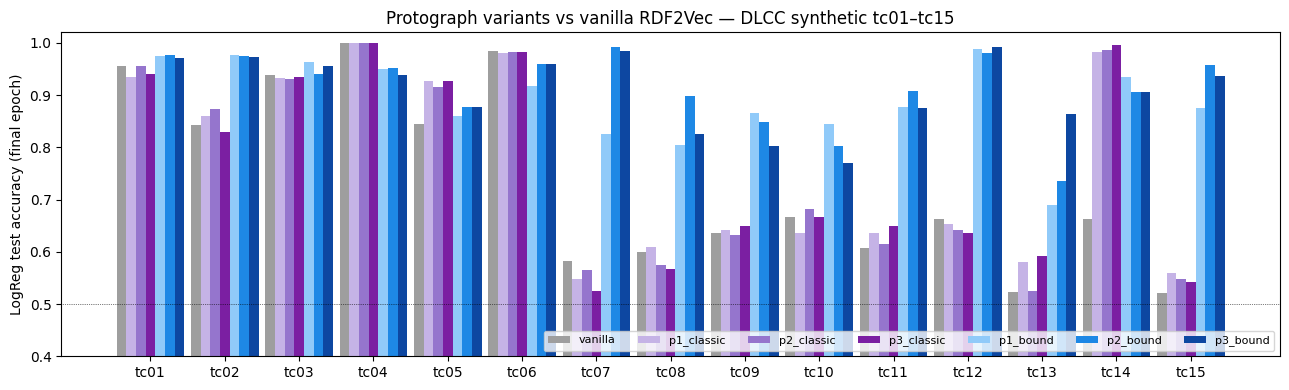
\includegraphics[width=\textwidth]{assets/compare/final_accuracy_tc01_tc15.png}
    \caption{Final test accuracy on the fifteen synthetic DLCC test cases
    (tc01--tc15) for all variants of the comparison run.}
    \label{fig:compare_final_tc01_tc15}
\end{figure}

\begin{figure}[t]
    \centering
    \makebox[\linewidth][c]{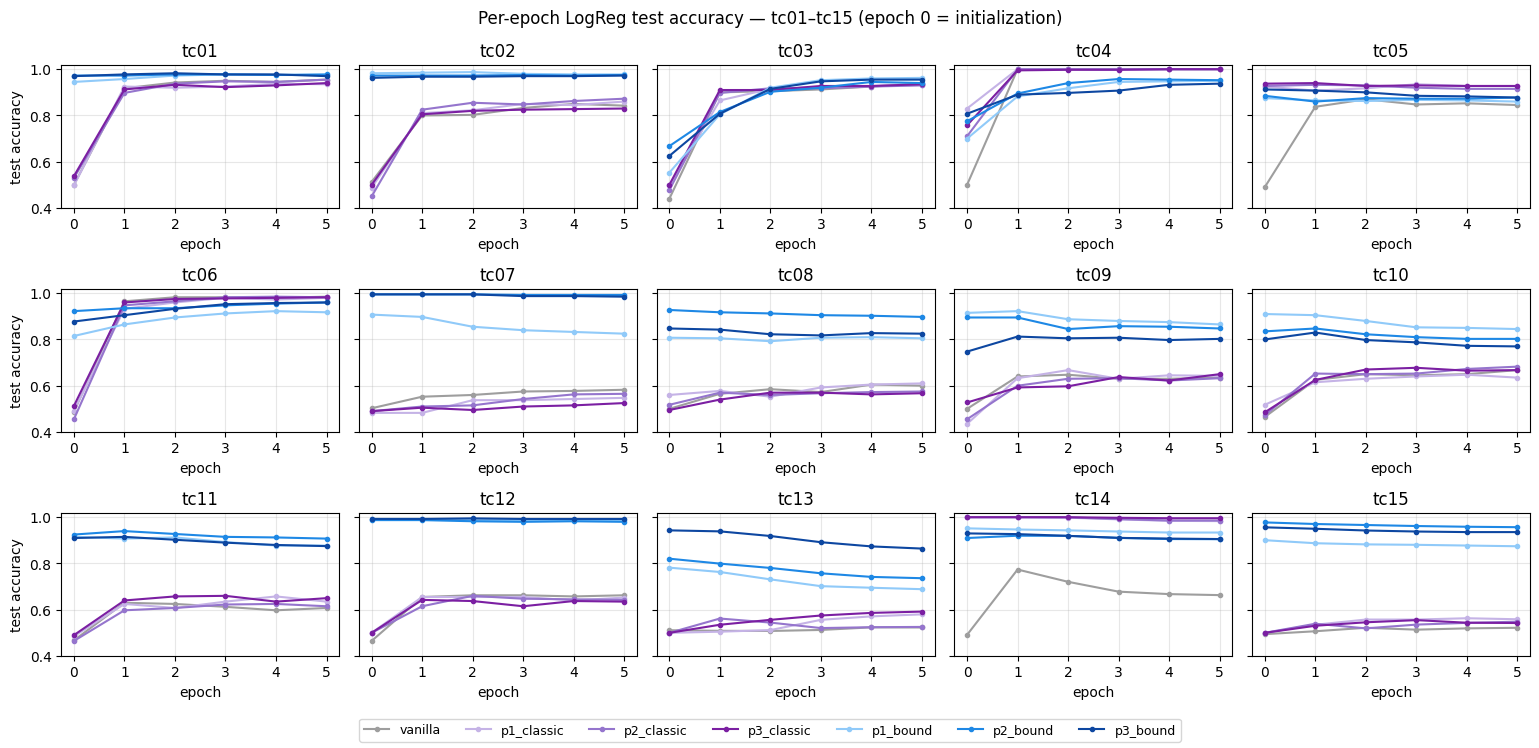
\includegraphics[width=\dimexpr\paperwidth-3cm\relax]{assets/compare/epoch_curves_tc01_tc15.png}}
    \caption{Per-epoch test accuracy on the fifteen synthetic DLCC test cases
    (tc01--tc15) for all variants of the comparison run. All variants use
    200-dimensional skip-gram embeddings, depth-3 duplicate-free walks, a shared
    target norm of $8$ and seed $42$; accuracy is the DLCC logistic-regression
    score on the held-out test entities, reported after each of the $5$
    fine-tuning epochs. The concept-bound variants are fine-tuned at the
    protected learning rate $0.0025$, while \texttt{vanilla} and the classic
    variants use the from-scratch rate $0.025$. The bound variants start high and
    stay nearly flat under the protected rate; the classic variants start at
    chance and barely move.}
    \label{fig:compare_epochs_tc01_tc15}
\end{figure}

\begin{figure}[t]
    \centering
    \makebox[\linewidth][c]{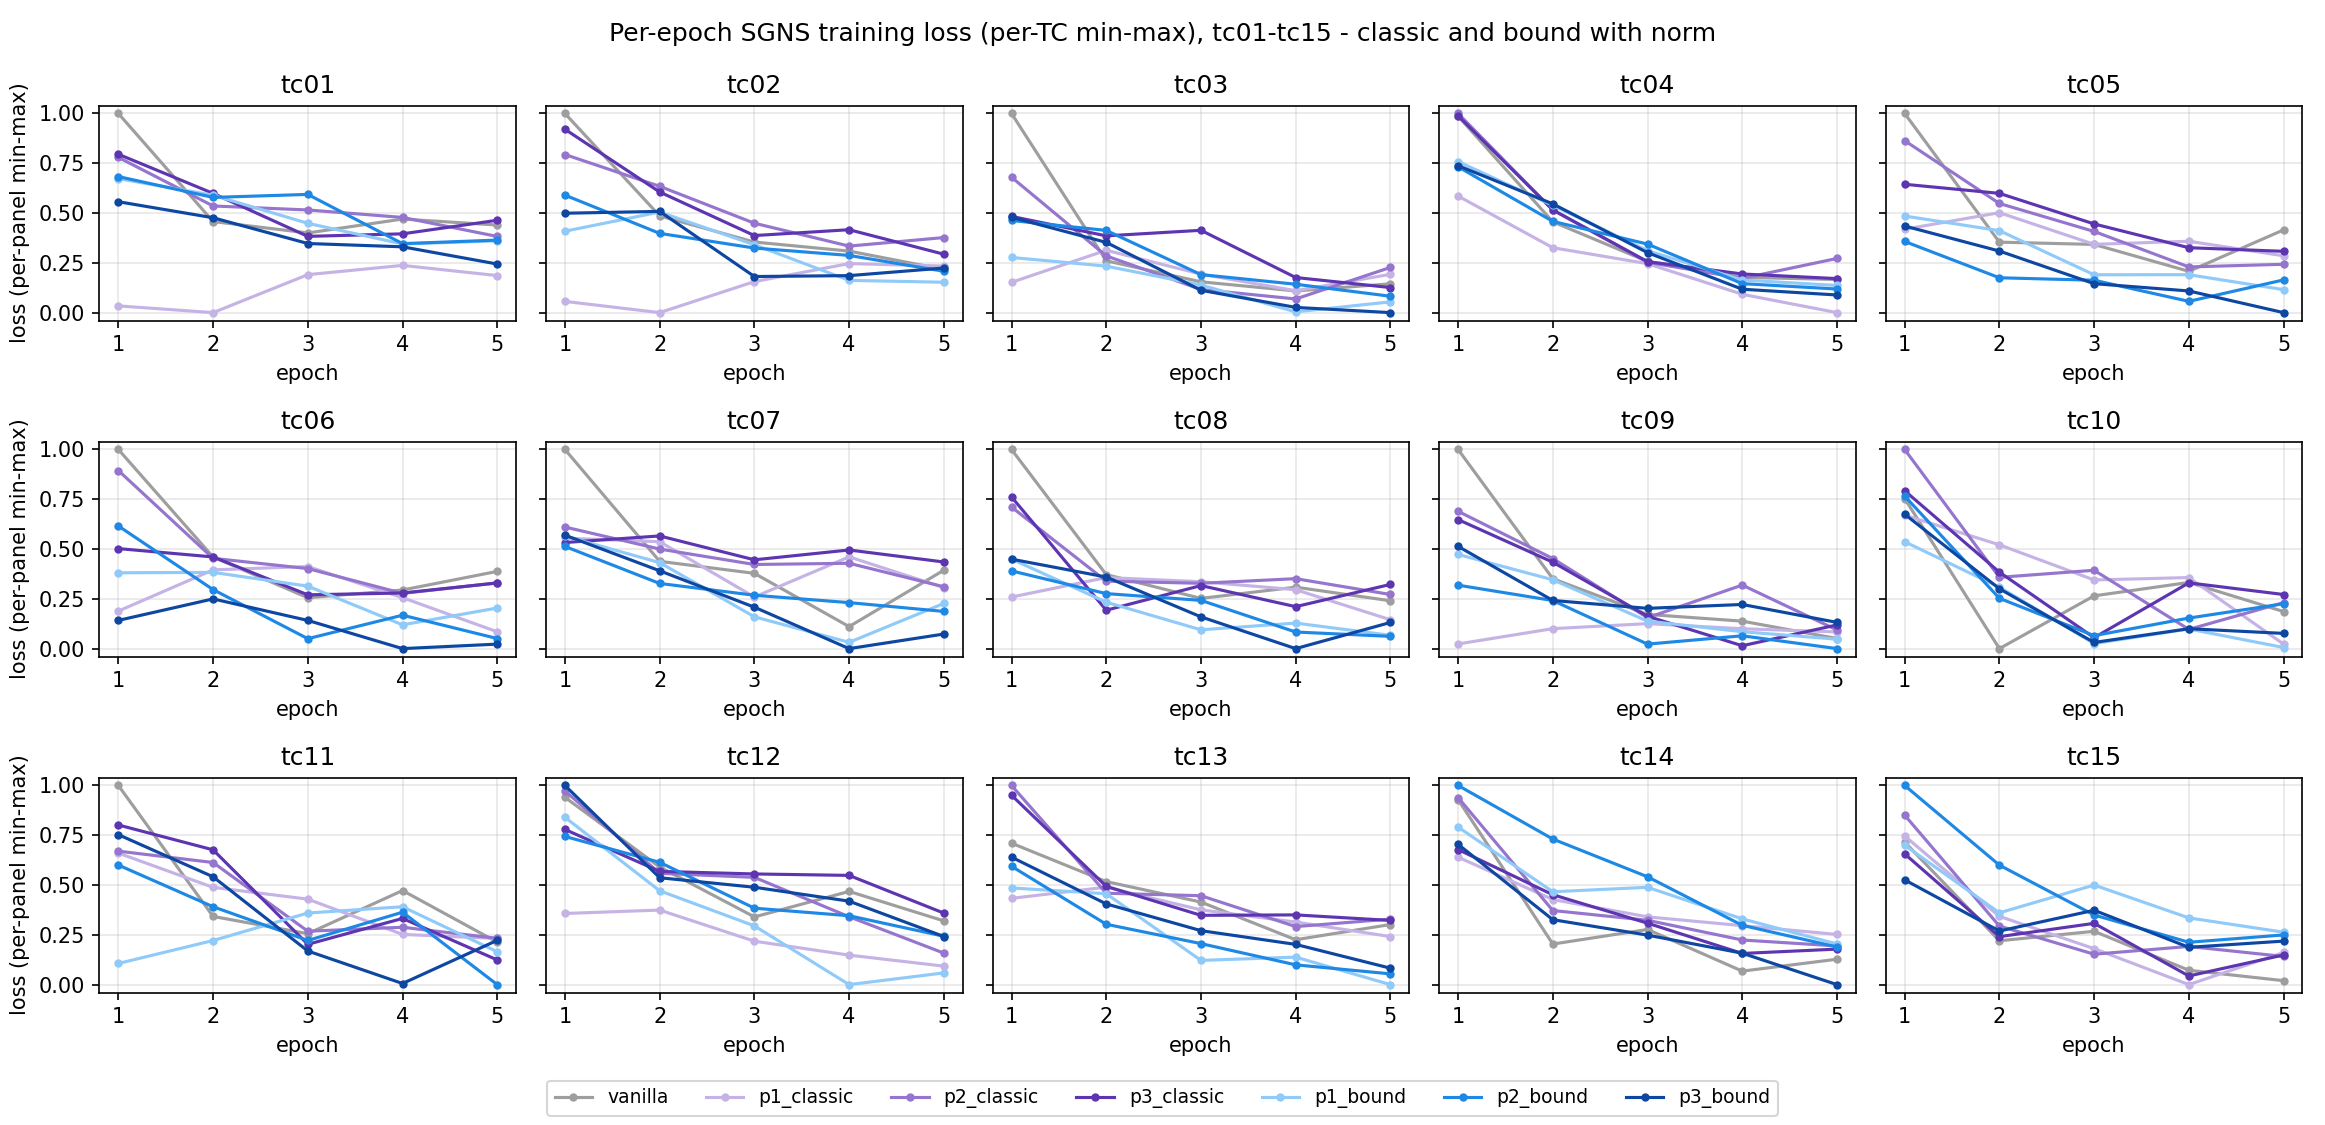
\includegraphics[width=\dimexpr\paperwidth-3cm\relax]{assets/compare/epoch_loss_classic_norm8_bound_tc01_tc15.png}}
    \caption{Per-epoch RDF2Vec fine-tuning loss on tc01--tc15 for \texttt{vanilla},
    the classic transfer (\texttt{most\_specific}) and the concept-bound variants,
    all initialized from the normalized (norm $8$) codes; \texttt{vanilla} and the
    classic transfer use the from-scratch learning rate $0.025$, the
    concept-bound variants the protected $0.0025$. Each panel is min--max
    normalized to $[0,1]$ per test case (y-axes are not shared). The classic
    curves that rise rather than fall are an artifact of the norm-$8$
    initialization, not of learned quality; without normalization they descend
    monotonically (Section~\ref{sec:results_norm_ablation},
    Appendix~\ref{app:norm-ablation}).}
    \label{fig:compare_epoch_loss_tc01_tc15}
\end{figure}




Three findings summarize the table.

\textbf{The concept-bound initialization solves the relation-centric tasks
that all previous variants fail.} On tc07--tc12 the best bound variant lifts
mean accuracy from 0.626 (\texttt{vanilla}) and 0.641 (best classic) to 0.905
(\texttt{p2\_bound}), with the largest individual gains on tc07
($0.583 \rightarrow 0.993$) and tc12 ($0.662 \rightarrow 0.980$). The classic
variants confirm the structural analysis of
Section~\ref{sec:classic_limits}: even at the from-scratch fine-tuning rate they
only match the vanilla baseline on the focus set (\texttt{p1\_classic} mean 0.607
vs.\ 0.626, \texttt{p3\_classic} 0.638), because the classic transfer carries no
relation-specific signal for these tasks.

\textbf{The signal is present from the first epoch, not learned by fine-tuning.}
The per-epoch curves (Figure~\ref{fig:compare_epochs_tc01_tc15}) show the bound
variants already near their final accuracy at epoch~1 and staying essentially
flat under the protected fine-tuning rate, whereas the classic and \texttt{vanilla}
variants start near chance on the relation-centric tasks and barely move across the
five epochs. The loss plot (Figure~\ref{fig:compare_epoch_loss_tc01_tc15}) tells
the same story from the optimization side: the classic loss curves are decoupled
from test accuracy, and their shape is an artifact of the normalized
initialization (Section~\ref{sec:results_norm_ablation}) rather than evidence of
useful learning.

\textbf{The tasks the classic transfer already solves are preserved.} On the
enumerated-individual cases tc05 and tc06 and the class-membership case tc14, the
bound variants stay high (0.86--0.96) and never collapse, so the additional terms
do not hurt the tasks the classic transfer already solves. On tc14 the classic
variants stay near-perfect (\texttt{p3\_classic} 0.996, \texttt{p1\_classic}
0.986, \texttt{p2\_classic} 0.982) because the label \emph{is} the entity's own
class, while the bound variants pay a small price (0.905--0.934) for mixing in
neighbour features.

\section{Runtime}
\label{sec:results_runtime}

The concept-bound construction adds little cost. Averaged over the synthetic
test cases, the \texttt{p2\_bound} pipeline takes 25.5\,s end-to-end, of which
fine-tuning dominates with 20.8\,s (81\%); the initialization stage (transfer of
the pretrained codes plus the concept-bound construction) takes 2.4\,s
($\approx$9\%), of which the construction proper is $\approx$2.25\,s (the classic
transfer alone costs $\approx$0.14\,s), and protograph pretraining is shared
with the classic variants (P1: 0.3\,s, P2: 2.0\,s, P3: 1.8\,s on tc01).
All RDF2Vec stages were run with 16 worker threads, so the absolute
fine-tuning seconds scale with the thread count, whereas the relative split
across stages does not.
Because the bound and classic variants share the same walk corpora,
vocabulary build, and fine-tuning stage, the proposed method's overhead over
classic MASCHInE transfer is the bound construction alone, a few percent
of total runtime, while the accuracy difference on the focus test cases is
$\approx$26 points (Table~\ref{tab:synthetic_final}). Walk generation and
caching costs are identical across variants and excluded from these numbers.
Figure~\ref{fig:runtime_total_lines} plots the end-to-end total runtime per
test case for the three pipelines (\texttt{classic} and \texttt{bound} averaged
over their P1/P2/P3 variants): the curves stay close throughout, confirming
that the schema-informed initializations add only marginal overhead.

\begin{figure}[t]
  \centering
  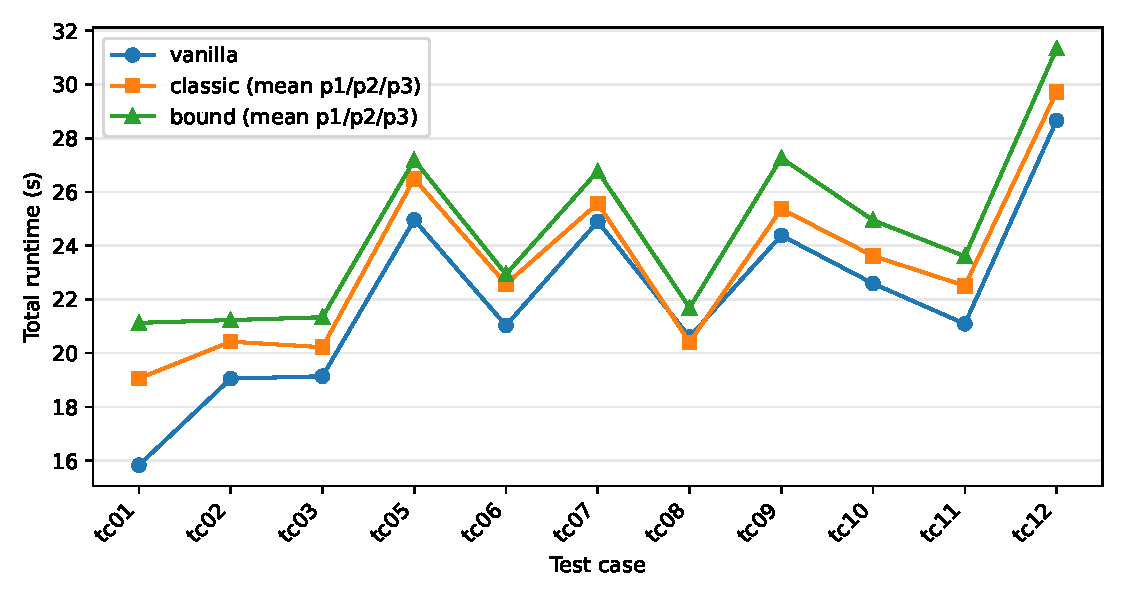
\includegraphics[width=\linewidth]{assets/runtime_total_lines.pdf}
  \caption{End-to-end total runtime per test case (seconds) for the three
  pipelines: \texttt{vanilla}, \texttt{classic}, and \texttt{bound}. The
  \texttt{classic} and \texttt{bound} lines are the means over their P1/P2/P3
  protograph variants. The three curves track closely at every test case -- the
  schema-informed variants stay within a few percent of \texttt{vanilla}, with
  fine-tuning dominating throughout. tc04 is omitted as a runtime outlier (its
  much larger walk corpus, $\approx$15$\times$, otherwise flattens the scale).
  Totals are taken from Table~\ref{tab:runtime_per_tc}
  (Appendix~\ref{app:runtime}).}
  \label{fig:runtime_total_lines}
\end{figure}

Table~\ref{tab:runtime_per_tc} (Appendix~\ref{app:runtime}) breaks the runtime
down per test case and variant into its three constituent stages, reported
separately and as an end-to-end total: protograph pretraining (RDF2Vec + code normalization),
instance-graph embedding initialization (transfer of pretrained codes, plus the
concept-bound construction for the \texttt{*\_bound} variants), and fine-tuning
(RDF2Vec on the instance walks). The \texttt{vanilla} baseline has no pretraining
and a random initialization, so only fine-tuning applies (marked ``--''
otherwise). Walk generation is excluded throughout, as is the
protograph-creation stage, which is negligible ($\approx$0.02--0.04\,s).
Pretraining and initialization cost a few seconds at most, and fine-tuning
dominates every variant, so the schema-informed variants total within a few
percent of \texttt{vanilla}. The full per-test-case breakdown is given in
Table~\ref{tab:runtime_per_tc} (Appendix~\ref{app:runtime}).

\section{Initialization and Coverage}
\label{sec:coverage}

We report the initialization coverage defined in
Section~\ref{sec:coverage_concept} at the vocabulary and
training-set levels and relate it to final accuracy.

Coverage increases from P1 to P2 to P3 at every level, and the two tables tell
the same story. At the vocabulary level
(Table~\ref{tab:vocab_init_coverage_tc01_tc15}, Appendix~\ref{app:vocab-coverage}),
P2 raises the share of protograph-initialized tokens over P1 by roughly 15--40
percentage points, and P3 reaches 100\% on every test case (\emph{Rand}~$=0$); P1
covers only 61--84\% of the vocabulary on the class-membership cases TC13--TC15. The
classifier's training split (Table~\ref{tab:train_class_init_coverage_tc01_tc15})
mirrors this exactly. P2 leaves far fewer randomly initialized entities than P1, and
P3 removes the remainder almost entirely, with the sharpest contrast on TC15, where
P1 initializes \emph{none} of the 200 training entities in either class while P2 and
P3 cover all of them.

\begin{table}[t]
\centering
\small
\caption{Training-set initialization by class for P1, P2, and P3 on TC01--TC15. Each cell reports protograph-initialized / random-initialized counts; the per-class training pool is 800 entities for TC01--TC12 and 200 entities for TC13--TC15 (counts below 800/200 indicate entities absent from the checkpoint vocabulary). The P1/P2 columns for TC01--TC12 are the originally reported figures; the P3 column and the TC13--TC15 rows are recomputed.}
\label{tab:train_class_init_coverage_tc01_tc15}
\resizebox{\textwidth}{!}{%
\begin{tabular}{lcccccc}
\toprule
\multirow{2}{*}{\textbf{TC}}
& \multicolumn{2}{c}{\textbf{P1 train split}}
& \multicolumn{2}{c}{\textbf{P2 train split}}
& \multicolumn{2}{c}{\textbf{P3 train split}} \\
\cmidrule(lr){2-3}
\cmidrule(lr){4-5}
\cmidrule(lr){6-7}
& \textbf{Positive} & \textbf{Negative}
& \textbf{Positive} & \textbf{Negative}
& \textbf{Positive} & \textbf{Negative} \\
\midrule
TC01 & 459/341 & 513/283 & 697/103 & 720/76 & 800/0 & 796/0 \\
TC02 & 445/355 & 452/348 & 698/102 & 713/87 & 800/0 & 800/0 \\
TC03 & 415/385 & 419/379 & 673/127 & 689/109 & 800/0 & 798/0 \\
TC04 & 586/214 & 598/201 & 757/43 & 740/59 & 800/0 & 799/0 \\
TC05 & 571/229 & 792/0 & 741/59 & 792/0 & 800/0 & 792/0 \\
TC06 & 431/369 & 410/390 & 659/141 & 659/141 & 800/0 & 800/0 \\
TC07 & 268/532 & 276/524 & 800/0 & 800/0 & 800/0 & 800/0 \\
TC08 & 486/314 & 488/312 & 710/90 & 707/93 & 800/0 & 800/0 \\
TC09 & 417/383 & 441/359 & 701/99 & 700/100 & 800/0 & 800/0 \\
TC10 & 396/404 & 369/431 & 703/97 & 685/115 & 800/0 & 800/0 \\
TC11 & 455/345 & 466/334 & 729/71 & 721/79 & 800/0 & 800/0 \\
TC12 & 0/800 & 0/800 & 0/800 & 0/800 & 800/0 & 800/0 \\
TC13 & 200/0 & 200/0 & 200/0 & 200/0 & 200/0 & 200/0 \\
TC14 & 200/0 & 200/0 & 200/0 & 200/0 & 200/0 & 200/0 \\
TC15 & 0/200 & 0/200 & 200/0 & 200/0 & 200/0 & 200/0 \\
\bottomrule
\end{tabular}%
}
\end{table}

Coverage does not, however, explain the accuracy differences in
Table~\ref{tab:synthetic_final}. Despite P1's substantially lower coverage at every
level, its classic-transfer accuracy is on par with the higher-coverage variants:
the means are 0.759 (P1), 0.768 (P2), and 0.774 (P3), all within about one and a
half points of one another and a few points above the 0.735 \texttt{vanilla} baseline, which uses no
protograph at all. Raising coverage from as little as 38\% under P1 to a full 100\%
under P3 thus leaves final accuracy essentially unchanged. This is a signal that the
schema information we inject into the instance embeddings at initialization is not
impactful for the DLCC tasks, however many entities it reaches: what the
initialization encodes matters more than how broadly it is applied.

TC12 makes the point in the extreme. P1 and P2 initialize 38.9\% and 78.8\% of
vocabulary tokens yet \emph{zero} classification entities, because the leaf classes
that type its instances never appear as a domain or range and so are absent from both
protographs; P3 materializes the full subclass hierarchy and covers every entity. Yet
classic accuracy stays close for the coverage extremes (0.655, 0.725, 0.672 for P1/P2/P3;
P1 with zero typed entities and P3 with full coverage land within two points), reinforcing the same
conclusion.

\subsection{Comparison of Initialization Strategies}
\label{sec:results_init_strategies}

Table~\ref{tab:init_strategies} reports a head-to-head comparison of the four
strategies of Section~\ref{sec:init_strategies}. All run on the same TC set under
one fixed budget, and vary \emph{only} which class vectors seed an instance. We
evaluate each strategy on all three protographs, because the strategies are
remedies for the leaf-class coverage gap: that gap is widest under P1, narrower
under P2, and already closed by P3. The outcome is unambiguous and, at first
sight, counter-intuitive. The three climbing strategies reach full ($100\%$)
initialization coverage, whereas \texttt{most\_specific} leaves $41\%$ of
instances at random init under P1 and $12\%$ under P2 (it already reaches $100\%$
on P3). Yet \emph{none of them improves final accuracy over
\texttt{most\_specific}}.

The pattern is consistent across protographs. On the richer P2 protograph,
\texttt{most\_specific} ($0.769$) and \texttt{all\_init} ($0.758$) are
effectively tied, while \texttt{weight\_hierarchy} ($0.743$) and especially
\texttt{average\_hier} ($0.641$) are clearly worse. On the sparse P1 protograph
the gap is dramatic ($0.752$ vs.\ $0.62$--$0.57$): aggressively filling coverage
there \emph{hurts} more than the random fallback it replaces. P3 is the decisive
control. There \texttt{most\_specific} \emph{already} seeds every instance from a
class vector, so it reaches $100\%$ coverage without any climbing. The climbing
strategies can therefore only redistribute coverage, not add it:
\texttt{all\_init} ($0.746$) merely matches \texttt{most\_specific} ($0.742$),
while the blending variants again fall away (\texttt{weight\_hierarchy} $0.681$,
\texttt{average\_hier} $0.589$). Tellingly, P3's complete coverage does not lift
\texttt{most\_specific} above its P2 value ($0.742$ vs.\ $0.769$).\footnote{This
strategy comparison (Table~\ref{tab:init_strategies}) is an independent
single-seed run from the headline comparison (Table~\ref{tab:synthetic_final}),
so its \texttt{most\_specific}/P3 mean ($0.742$) differs from
\texttt{p3\_classic} there ($0.774$) by about three points, at the edge of the
run-to-run noise floor (Section~\ref{sec:setup}); the P2-vs-P3 ordering is
correspondingly not stable across the two runs, so we read coverage, not the
exact ranking, as the point.} This is evidence that the coverage count is not
what drives accuracy.

One likely explanation is over-smoothing. Climbing the hierarchy replaces a
missing leaf-class embedding with a shared ancestor's embedding. Many instances
that were distinct under \texttt{most\_specific}, each random but
\emph{differently} random, then collapse onto the same handful of ancestor
vectors. The results fit this account. The uniform blend of
\texttt{average\_hier} dilutes most aggressively and is consistently the weakest.
\texttt{all\_init} is the safest climbing variant, because it only touches
out-of-vocabulary instances and keeps them at their nearest covered ancestor.

Two conclusions follow. First, the coverage problem that motivated these
strategies is real, but the obvious fix does not pay off. What matters is the
carrier of schema signal, not the coverage count, as argued in
Section~\ref{sec:method_overview}. Second, \texttt{most\_specific} is a sound
default, which is why our main experiments use it. No strategy meaningfully
improves on the from-scratch \texttt{vanilla} baseline ($0.739$):
\texttt{most\_specific} merely matches it, while the more aggressive hierarchy
traversals are at best on par (\texttt{all\_init} under P2 and P3) and often
clearly worse, dropping to $0.57$--$0.62$ under the sparse P1 protograph. Filling
coverage by blending in or substituting ancestor vectors thus tends to hurt
rather than help. The complete per-test-case breakdown behind the
\texttt{Acc@final} column, giving the final accuracy for every strategy,
protograph, and test case, is reported in Appendix~\ref{app:init-strategies}
(Table~\ref{tab:init_strategies_pertc}).

\begin{table}[t]
\centering
\caption{Quantitative comparison of the four class-hierarchy initialization strategies on the synthetic DLCC test cases \texttt{tc01}--\texttt{tc15}, under one fixed budget ($\dim=200$, 100 instance walks/entity, depth 3, $5+5$ epochs, $\lambda=0.5$, from-scratch fine-tuning rate $0.025$, single run per cell). \emph{Coverage} is the mean fraction of typed instances that receive a class-based initialization (rather than a random one); \emph{init} and \emph{final} are mean LogReg test accuracy at epoch 0 and epoch 5, averaged over all 15 test cases. The \texttt{vanilla} row is from-scratch RDF2Vec. This is an independent run from the headline Table~\ref{tab:synthetic_final}, so the \texttt{most\_specific} means differ slightly between the two (e.g.\ P3 $0.742$ here vs.\ \texttt{p3\_classic} $0.774$ there).}
\label{tab:init_strategies}
\begin{tabular}{llrrr}
\toprule
Protograph & Strategy & Coverage (\%) & Acc@init & Acc@final \\
\midrule
- & \texttt{vanilla} & -- & 0.488 & 0.739 \\
\midrule
P1 & \texttt{most\_specific} & 58.5 & 0.573 & 0.752 \\
P1 & \texttt{all\_init} & 100.0 & 0.576 & 0.621 \\
P1 & \texttt{average\_hier} & 100.0 & 0.565 & 0.565 \\
P1 & \texttt{weight\_hierarchy} & 100.0 & 0.576 & 0.574 \\
\midrule
P2 & \texttt{most\_specific} & 88.1 & 0.567 & 0.769 \\
P2 & \texttt{all\_init} & 100.0 & 0.564 & 0.758 \\
P2 & \texttt{average\_hier} & 100.0 & 0.567 & 0.641 \\
P2 & \texttt{weight\_hierarchy} & 100.0 & 0.572 & 0.743 \\
\midrule
P3 & \texttt{most\_specific} & 100.0 & 0.578 & 0.742 \\
P3 & \texttt{all\_init} & 100.0 & 0.578 & 0.746 \\
P3 & \texttt{average\_hier} & 100.0 & 0.570 & 0.589 \\
P3 & \texttt{weight\_hierarchy} & 100.0 & 0.577 & 0.681 \\
\bottomrule
\end{tabular}
\end{table}



\section{Embedding-Space Diagnostics}
\label{sec:results_diagnostics}

The accuracy table reports \emph{which} variants solve which test cases. This
section inspects the embedding spaces to explain \emph{why}. We focus on three
representative test cases and compare \texttt{vanilla}, \texttt{p1\_classic}, and
\texttt{p3\_bound}. The three cases are tc07 (qualified existential restriction
$\exists r.C$), tc09 (cardinality, one versus two outgoing edges of the target
relation), and tc14 (own-class membership). We read the held-out test entities
\emph{at initialization}, that is, before the first fine-tuning epoch. At that
point the differences between the initializations are not yet diluted by
training. 

\paragraph{Class distribution under a label-aware projection.}
To see whether the positive and negative entities occupy separable regions, we
project each method's test embeddings onto their first linear discriminant (LD1),
a label-aware axis. The full set of panels is collected in
Appendix~\ref{app:lda-all}. We use LDA rather than PCA on purpose. PCA shows the
directions of maximum \emph{variance}, which need not contain the label boundary.
A linearly separable embedding can therefore look thoroughly mixed in its leading
principal components whenever the discriminative direction carries little
variance. LDA instead chooses the axis that maximizes class separation. Under
this view, persistent mixing is direct evidence that no linearly separable signal
is present, not an artifact of an unlucky projection. On the relation-centric
tasks \texttt{vanilla} and the classic variants stay mixed even along this axis,
consistent with their near-chance accuracies (Table~\ref{tab:synthetic_final}),
whereas \texttt{p3\_bound} separates the two classes cleanly.

\paragraph{The classic transfer collapses entities onto class means.}
Section~\ref{sec:classic_limits} predicted this failure structurally; here it
becomes concrete. Under \texttt{p1\_classic}, the 400 test entities of tc07 share
only \emph{two} distinct initialization vectors, and those of tc09 only 176. The
cause is the initialization rule itself: each entity is seeded with the mean
embedding of its classes, and the labeled entities share almost all of their
class memberships, so their seeds collapse onto a handful of points. The labels
on tc07--tc12, however, do not depend on an entity's own class. A collapsed
initialization therefore cannot tell apart entities that differ only in their
label, and fine-tuning cannot recover a signal that the initial vectors never
carried. This is why the corresponding accuracy curves stay flat at chance level
(Figure~\ref{fig:compare_epochs_tc01_tc15}). \texttt{p3\_bound}, by contrast,
keeps all 400 vectors distinct and arranges them into label-consistent regions.

\paragraph{The margin exists before fine-tuning.}
Figure~\ref{fig:diag_violins} projects each embedding onto its discriminant axis
(LD1, standardized per panel) and compares the per-class distributions. For
\texttt{p3\_bound} the two classes form clearly separated, near-bimodal
distributions on all three test cases at epoch 0. The logistic regression only
has to read off a margin that the initialization already provides, which is why
the bound accuracy curves start high and stay flat. The \texttt{vanilla} panels show a partial gap between the two classes, but it
is spurious: with only 400 points in 200 dimensions, the discriminant axis can
separate them in-sample even when no real structure is present. The held-out
accuracy at initialization stays at chance, which confirms the gap is an
overfitting artifact. \texttt{p1\_classic} either overlaps (tc07, tc09) or, on tc14, collapses every
entity onto one of two vectors, the means of its two classes. Because the tc14
label is the entity's own class, those two means line up one-to-one with the two
labels by construction, so the classes are perfectly separated already at
initialization.

\begin{figure}[p]
    \centering
    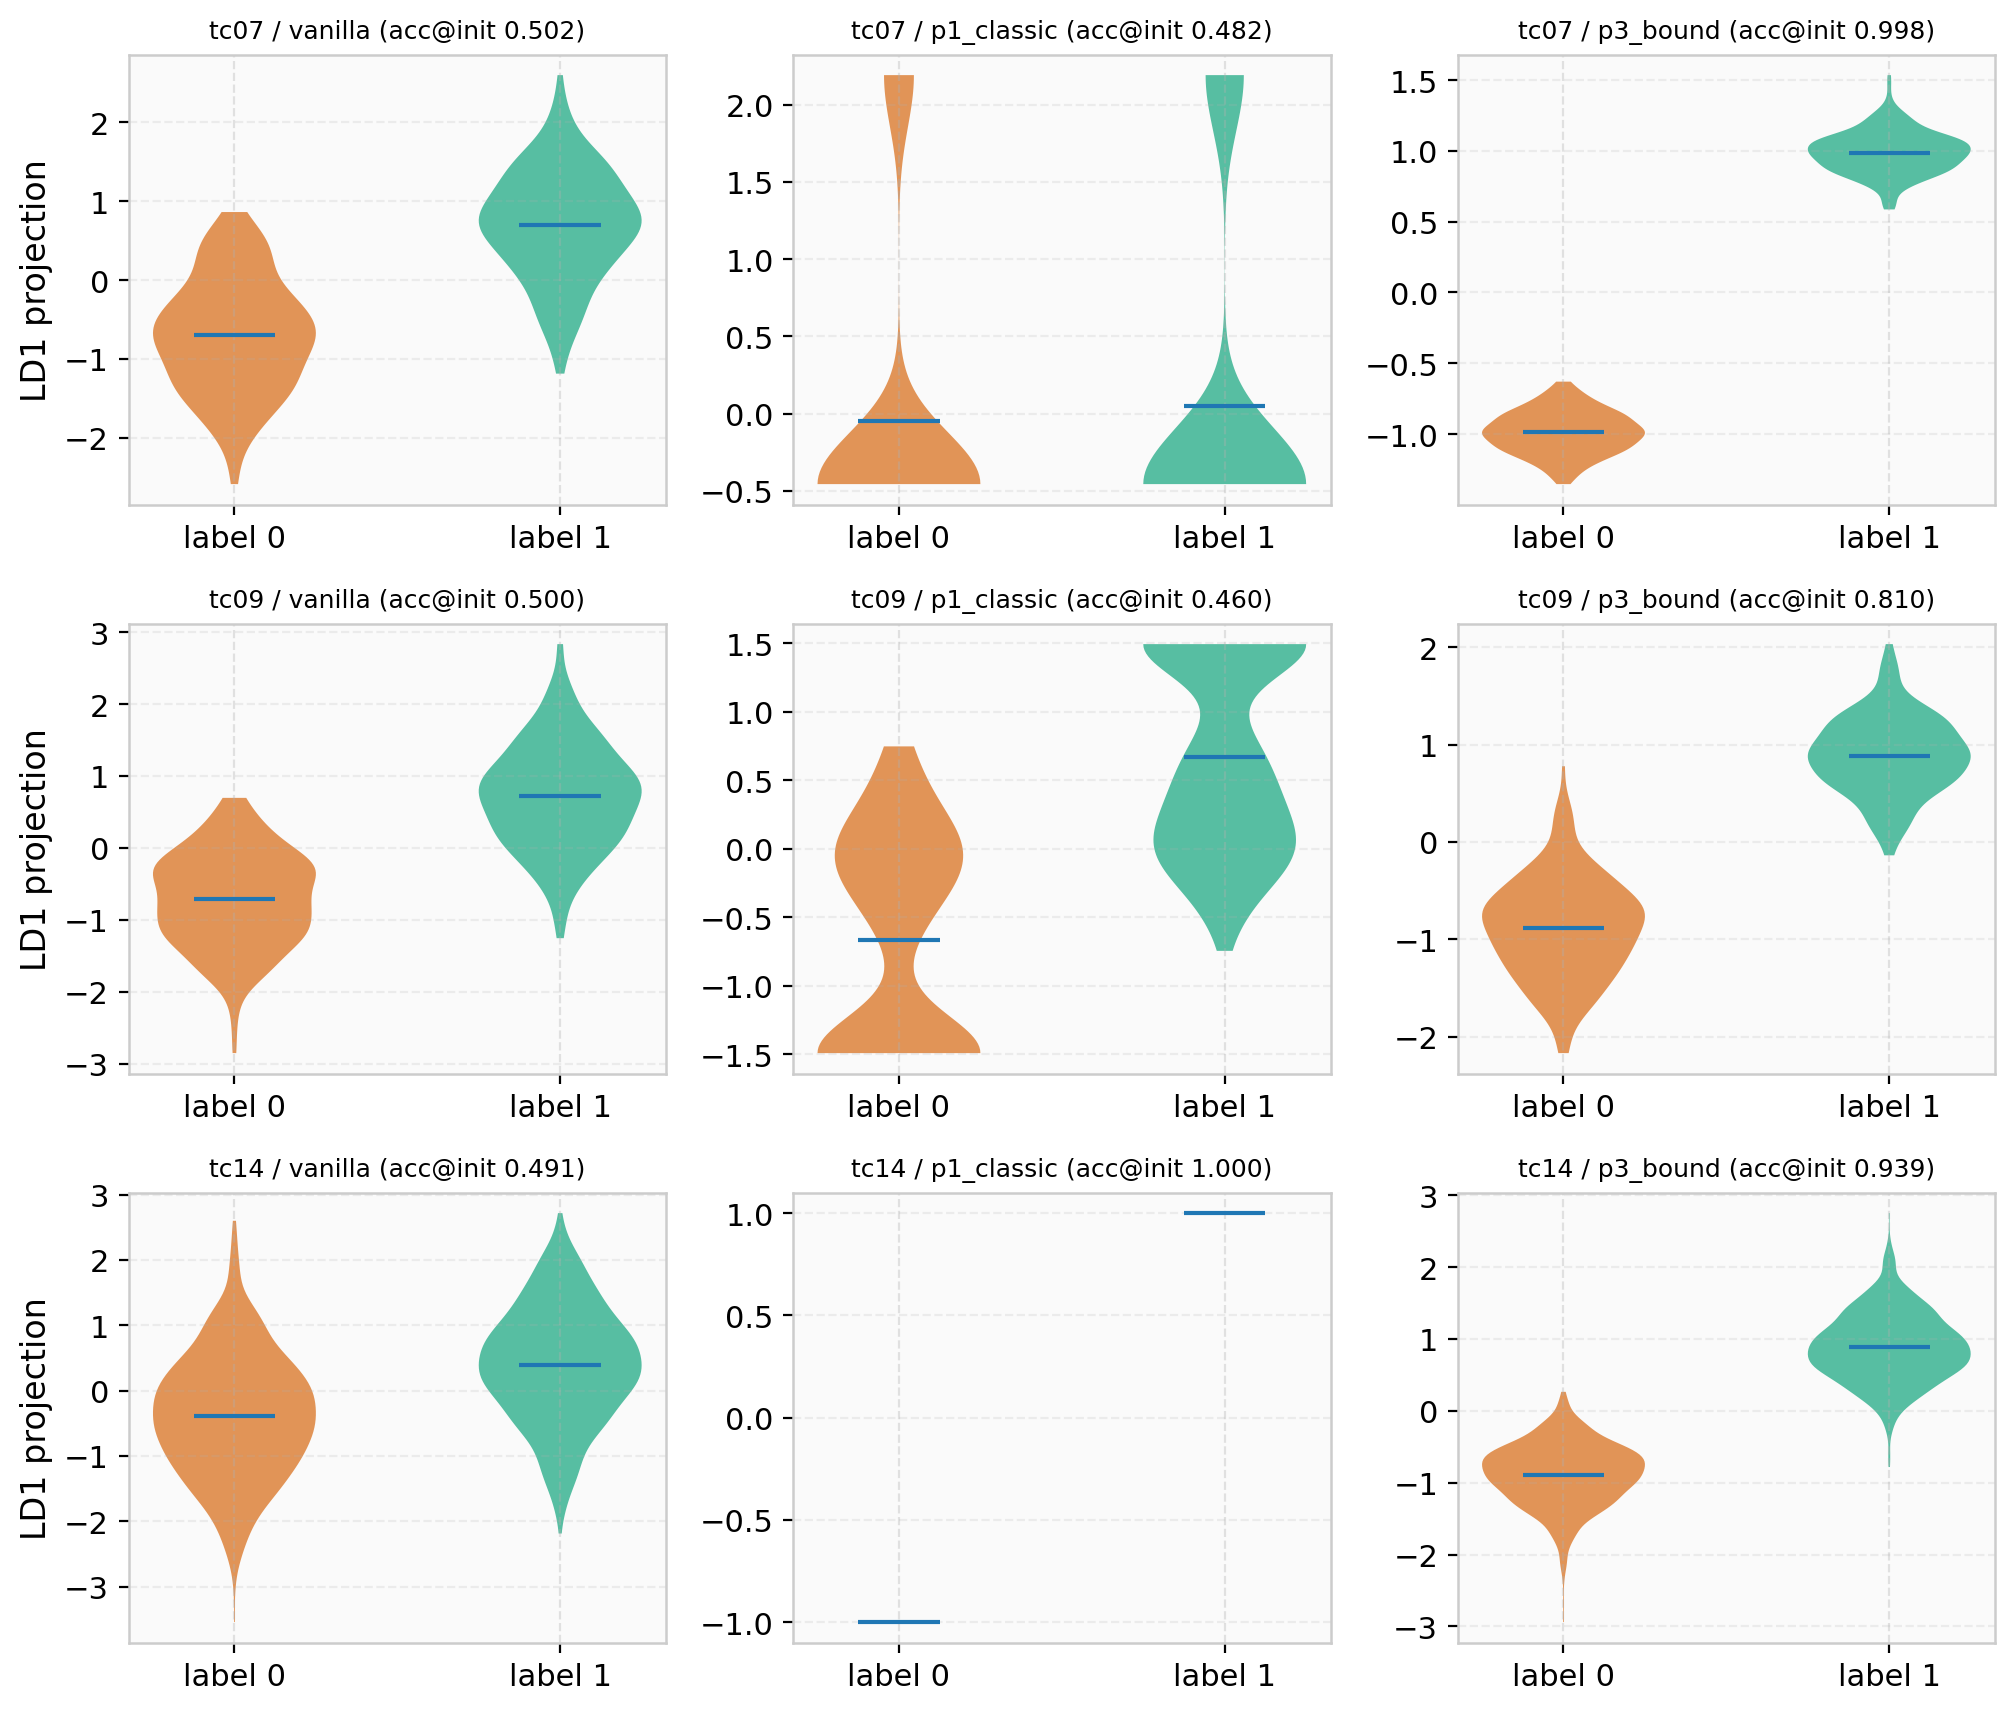
\includegraphics[width=0.92\textwidth]{assets/visuals/ld1_violins.png}
    \caption{Distribution of the test-entity embeddings along the
    standardized discriminant axis (LD1) at initialization, per test case
    (rows) and variant (columns). Separated violins mean the label is
    linearly readable before any fine-tuning. The apparent gap for
    \texttt{vanilla} is discriminant overfitting (held-out accuracy is at
    chance); on tc14 / \texttt{p1\_classic} the two spikes are the two class
    means, which coincide with the label by construction.}
    \label{fig:diag_violins}
\end{figure}

One scalar captures how far an initialization moves during fine-tuning: the mean
cosine between the epoch-0 and epoch-5 vectors. \texttt{vanilla}, trained at the
from-scratch learning rate, is essentially re-randomized (cosine $\leq 0.05$). The
\emph{concept-bound} variants, fine-tuned at the reduced learning rate, barely
move (cosine typically $\geq 0.85$). The \emph{classic} variants sit in between,
and how far they move depends on the protograph. The heavily collapsed
\texttt{p1\_classic} transfer hardly moves, while \texttt{p2\_classic} and
\texttt{p3\_classic} move far. This only matters for the bound variants, whose
starting point already carries the label signal. The classic start carries none,
so it stays at chance whether it moves or not. The next subsection shows this
drift entity by entity.

\subsection{Forgetting and Fine-Tune Drift}
\label{sec:results_drift}
\label{sec:forgetting}

A natural suspicion is that the pretrained signal is present at initialization
but destroyed by fine-tuning. The from-scratch learning rate of $0.025$ was tuned
for random initializations, not for preserving transferred structure. To make the
drift visible per entity, Figure~\ref{fig:pca_drift_all_tcs} projects the
test-entity embeddings of the representative test case tc07 onto a shared
per-panel PCA basis, fitted on the union of the epoch-0 and epoch-5 vectors. An
arrow connects each entity's initialization to its position after five
fine-tuning epochs. The figure contrasts the \texttt{vanilla} RDF2Vec baseline,
which has no protograph initialization and trains from scratch, with the six
protograph variants. The top row places the \texttt{vanilla} baseline next to the
three \emph{classic} initializations, fine-tuned at the from-scratch learning rate
$0.025$. The bottom row shows the three \emph{concept-bound} initializations under
the protected learning rate $0.0025$. The equivalent figures for the remaining
fourteen test cases (tc01 to tc06 and tc08 to tc15) are collected in
Appendix~\ref{app:pca-drift-all}.

The two learning rates produce a clear contrast. The concept-bound variants under
the protected learning rate barely move. Their arrows are short, the epoch-5 cloud
sits almost on top of the epoch-0 cloud, and the per-entity cosine is typically
$\geq 0.85$, so the bound features survive fine-tuning intact. Under the
from-scratch learning rate the picture is mixed. On most protographs the classic
vectors travel far, with long arrows and low cosines, so whatever structure the
initialization provided is overwritten. This is the forgetting seen
entity by entity. On the most collapsed transfer, \texttt{p1\_classic}, the
vectors instead barely move, but here there is nothing to preserve: the start has
collapsed onto a couple of points and carries no label signal. Either way the
classic result stays at chance. For the bound variants the short arrows protect a
start that is already label-consistent. Preserving the initialization is therefore
only useful when the initialization carries signal, which is the case the
protected fine-tuning recipe of Section~\ref{ch:method} is built for. It keeps the
label-consistent geometry of Figure~\ref{fig:diag_violins} from being washed out.

\begin{figure}[ht]
  \centering
  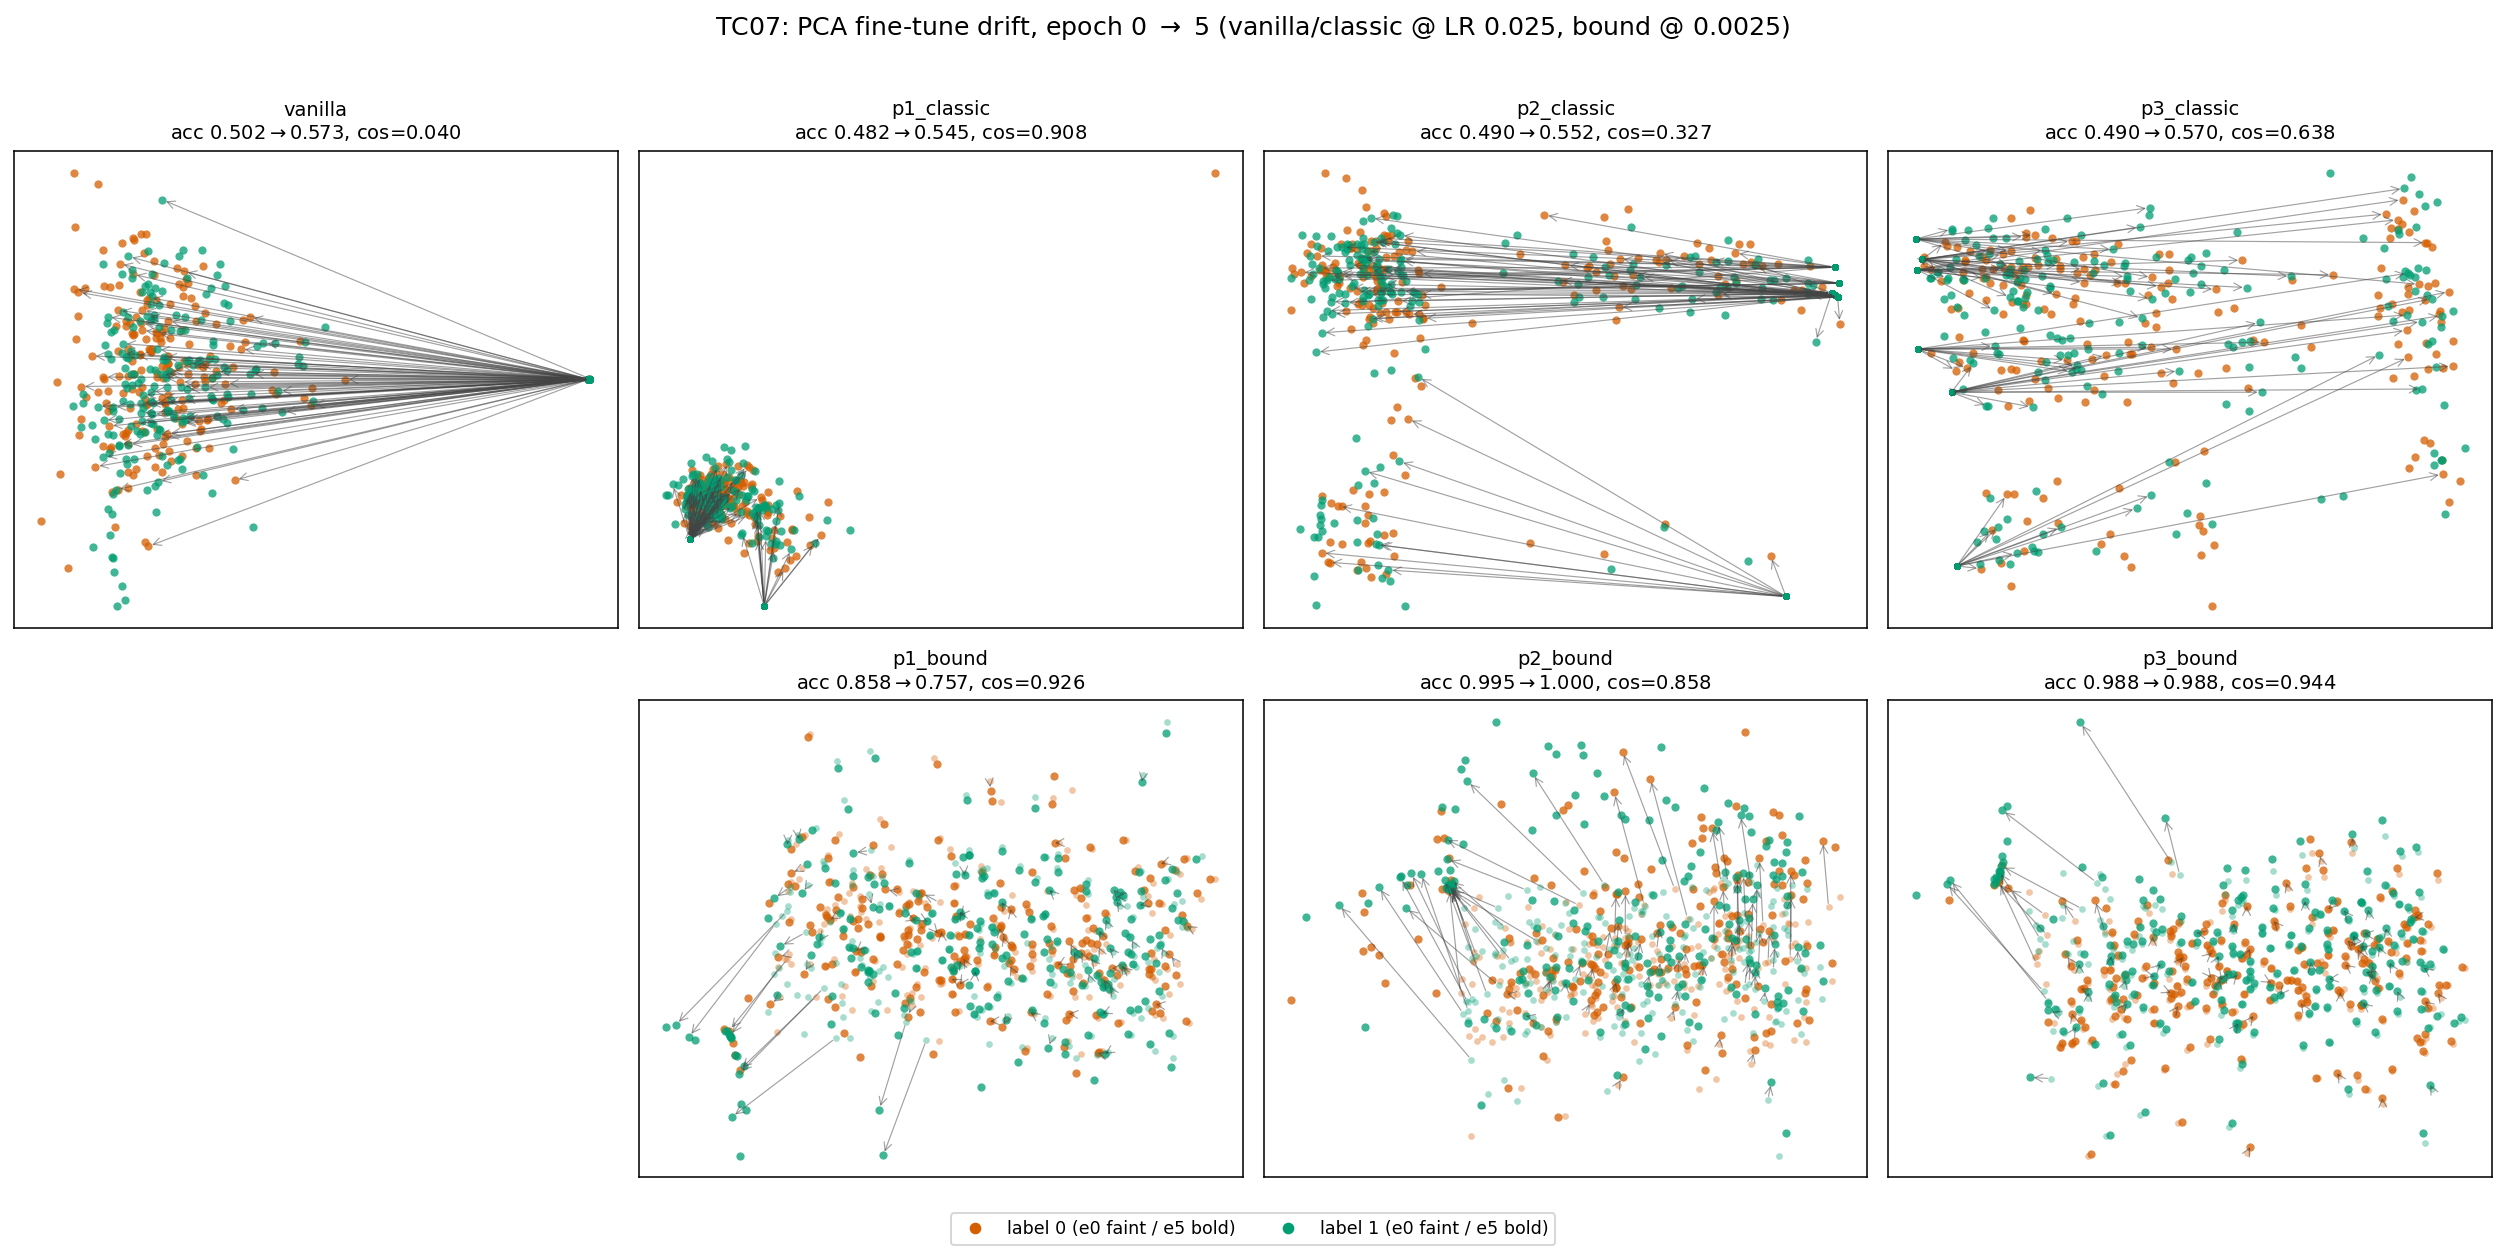
\includegraphics[width=0.98\textwidth]{assets/pca_drift/tc07_pca_drift.png}
  \caption{PCA fine-tune drift (epoch 0 $\rightarrow$ epoch 5) of the held-out
  test entities for the representative test case TC07 (qualified existential
  restriction $\exists r.C$). Each panel shares a PCA basis fitted on the union
  of the epoch-0 (faint) and epoch-5 (bold) vectors; arrows connect each
  entity's initialization to its fine-tuned position. Top-left: the
  \texttt{vanilla} RDF2Vec baseline (no protograph initialization, trained from
  scratch at learning rate $0.025$); rest of the top row: classic
  initializations (P1/P2/P3) fine-tuned at the same from-scratch learning rate
  $0.025$; bottom row: concept-bound initializations (P1/P2/P3) under the
  protected learning rate $0.0025$. Panel titles report accuracy at
  initialization $\rightarrow$ after fine-tuning and the mean epoch-0/epoch-5
  cosine. The equivalent figures for the remaining fourteen test cases
  (tc01--tc06 and tc08--tc15) are collected in
  Appendix~\ref{app:pca-drift-all}.}
  \label{fig:pca_drift_all_tcs}
\end{figure}

The same drift is visible as a scalar across the fine-tuning epochs.
Figure~\ref{fig:embedding_drift_tc01_tc12} reports the embedding drift
$1 - |\cos(\mathbf{v}_0, \mathbf{v}_t)|$ between the initial embedding
$\mathbf{v}_0$ and the embedding after fine-tuning epoch $t$, for all seven
variants on three representative test cases (tc01, tc07 and tc10); the remaining
twelve test cases are deferred to Appendix~\ref{app:cosine-drift-all} and show
the same pattern. \texttt{vanilla} jumps almost to full drift within
a single epoch. Where the classic transfer drifts, it does so early, leaving its
starting position within the first one to two epochs. The concept-bound curves
stay low throughout, which confirms epoch by epoch that the protected fine-tuning
preserves the transferred structure.

\begin{figure}[p]
    \centering

    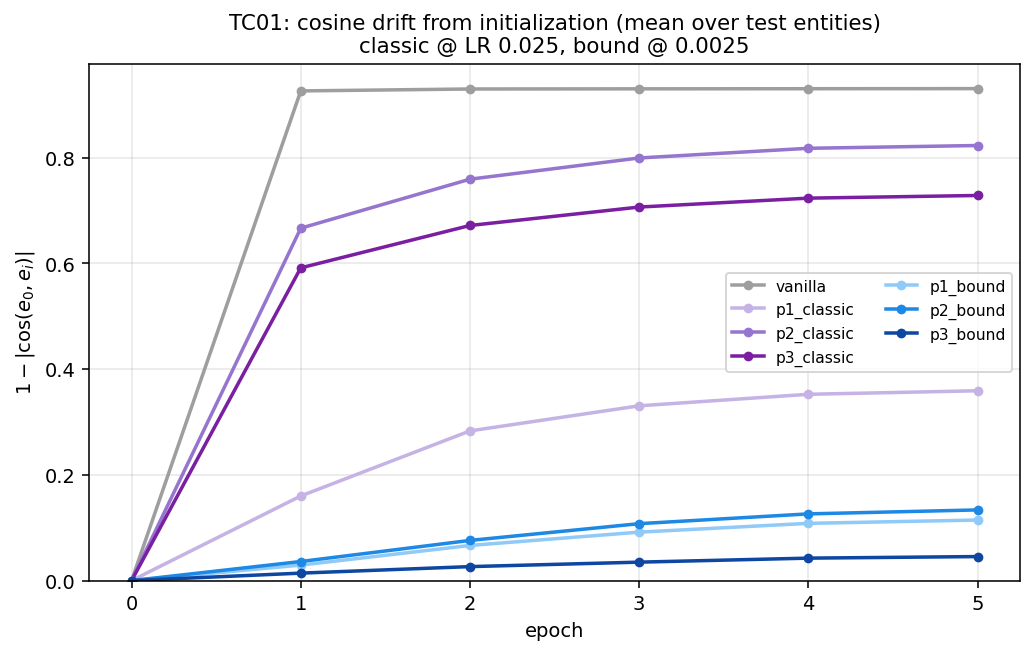
\includegraphics[width=0.62\textwidth]{assets/cosine_drift/tc01_cosine_drift.png}\\[0.8em]
    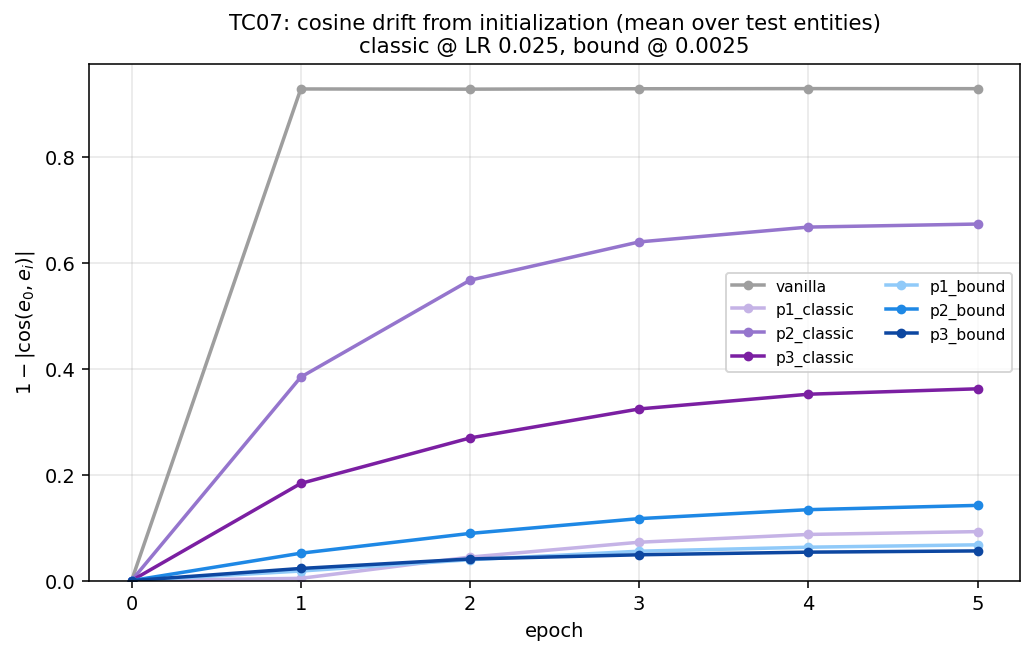
\includegraphics[width=0.62\textwidth]{assets/cosine_drift/tc07_cosine_drift.png}\\[0.8em]
    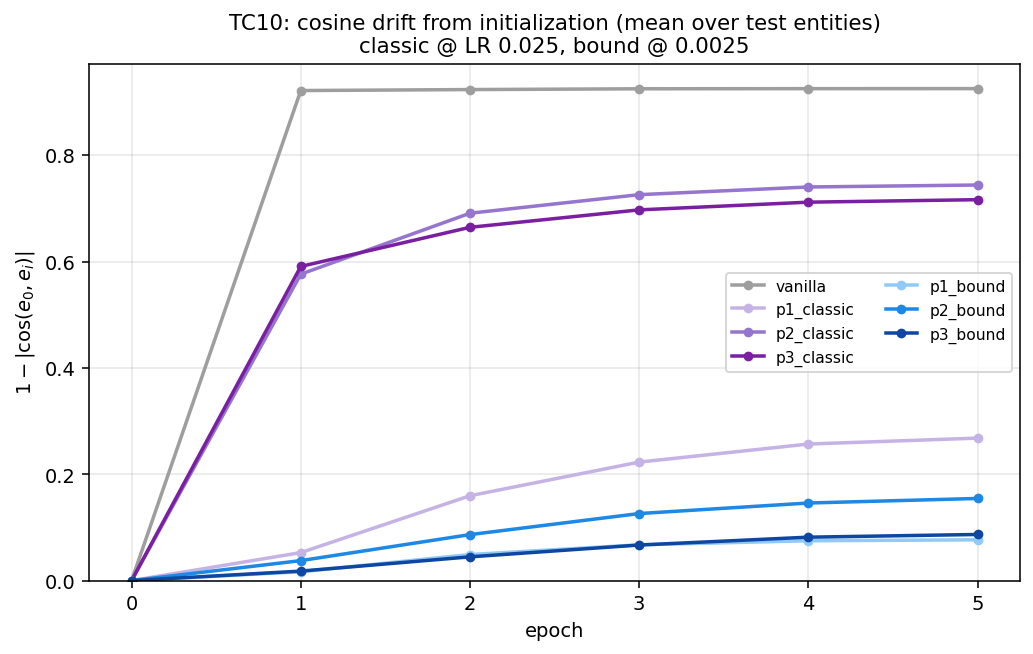
\includegraphics[width=0.62\textwidth]{assets/cosine_drift/tc10_cosine_drift.png}

    \caption{Embedding drift over fine-tuning epochs for all seven variants on three representative DLCC synthetic test cases (tc01, tc07, tc10); the full benchmark of all fifteen test cases is given in Appendix~\ref{app:cosine-drift-all}. Drift is measured as $1 - |\cos(\mathbf{v}_0, \mathbf{v}_t)|$, where $\mathbf{v}_0$ is the initial embedding and $\mathbf{v}_t$ is the embedding after fine-tuning epoch $t$. The classic variants use the from-scratch learning rate $0.025$ and the concept-bound variants the protected rate $0.0025$.}
    \label{fig:embedding_drift_tc01_tc12}
\end{figure}


\section{Ablation Results}
\label{sec:results_ablations}

We now isolate the contribution of each design choice introduced in Section~\ref{sec:ablations}, one ablation per subsection.

\subsection{Fine-Tuning Learning Rate}
\label{sec:results_lr}

The fine-tuning learning rate balances adapting the embeddings to the instance
graph against preserving the transferred schema structure
(Section~\ref{sec:abl_lr}). We compare the two rates already in our pipeline: the
\emph{protected} rate $0.0025$ used by the concept-bound variants
(Section~\ref{sec:norm}) and the \emph{from-scratch} rate $0.025$ used by
\texttt{vanilla}, applying each to all three classic transfers under the
comparison budget of Section~\ref{sec:setup}. Figure~\ref{fig:lr_ablation}
reports the mean final Logistic Regression test accuracy over
\texttt{tc01}--\texttt{tc15}; per-test-case values are in
Appendix~\ref{app:lr-ablation} (Table~\ref{tab:lr_ablation}).

Lowering the rate from $0.025$ to $0.0025$ helps no classic transfer:
\texttt{p2\_classic} is essentially unchanged ($0.765 \rightarrow 0.759$, within
noise), \texttt{p3\_classic} loses a small amount ($0.774 \rightarrow 0.741$),
and \texttt{p1\_classic} collapses ($0.758 \rightarrow 0.609$). At the
from-scratch rate all three sit at or just above the \texttt{vanilla} baseline
($0.736$);\footnote{Each experiment recomputes \texttt{vanilla} as an independent
single-seed run, so its mean over \texttt{tc01}--\texttt{tc15} fluctuates between
$0.735$ (Table~\ref{tab:synthetic_final}), $0.736$ (here), and $0.739$
(Table~\ref{tab:init_strategies}); the spread is below half a percentage point,
well within the ${\approx}3$ pp noise floor of
Appendix~\ref{app:stability-analysis}.} at the protected rate \texttt{p1\_classic}
falls well below it.

The reason is that the small rate freezes the transfer in place. The classic
init copies each class code into both weight matrices at norm $8$, so a step of
$0.0025$ moves the embeddings only slightly and they stay close to where they
started. This is the intended behaviour for the concept-bound init, but it hurts
the classic transfer: there every instance of a class starts from the same
vector, and these vectors have to move to capture instance-level structure
before the DLCC classifier can read it. Stuck near its weakest starting point,
\texttt{p1\_classic} stays near chance on the harder tasks (\texttt{tc03}
$0.500$, \texttt{tc08} $0.510$, \texttt{tc09} $0.450$) and its mean drops to
$0.609$; the from-scratch rate frees training again and recovers it to $0.758$.

The protected low rate is therefore something the concept-bound construction
needs, not a generally safe choice, so the classic variants use the from-scratch
rate $0.025$ throughout (Table~\ref{tab:synthetic_final}). Even at its best rate
the classic transfer only \emph{matches} \texttt{vanilla}: the schema signal
gives a better starting point but no lasting gain once fine-tuning is free to
move the embeddings.

\begin{figure}[t]
  \centering
  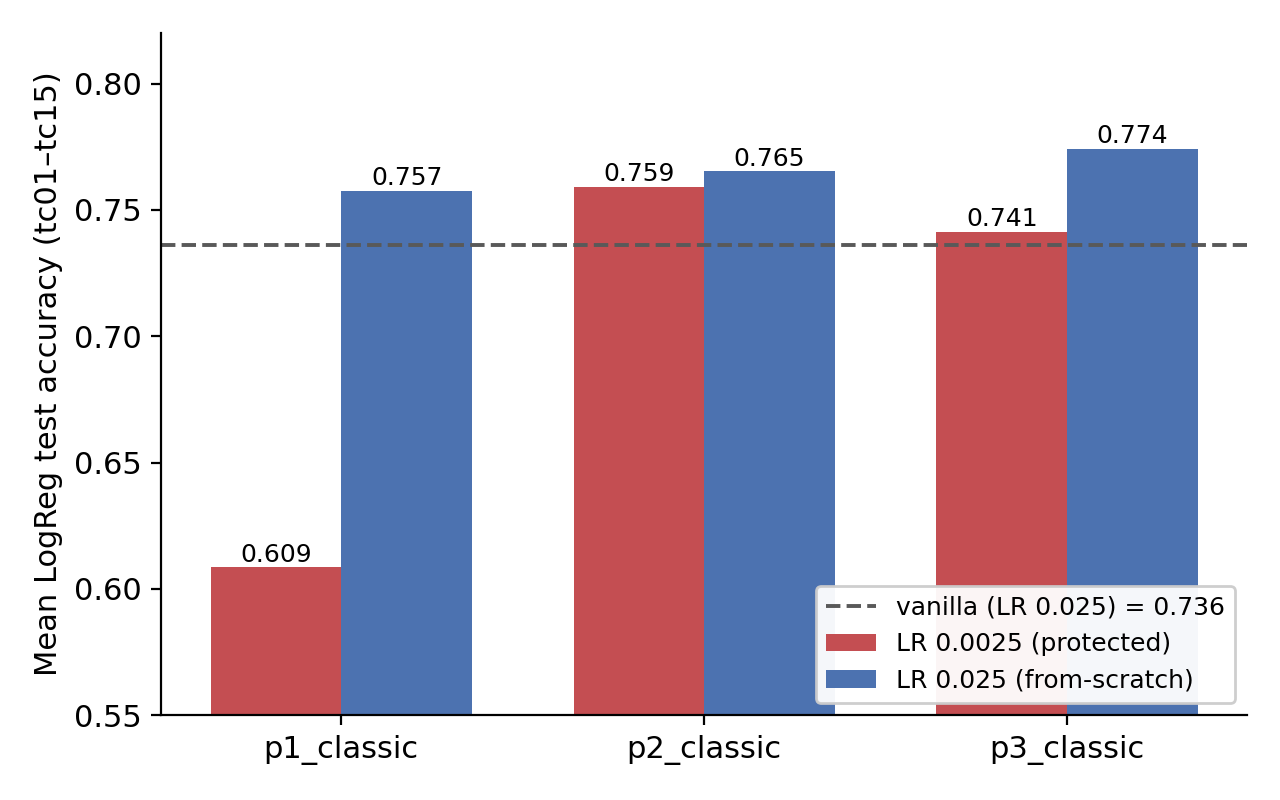
\includegraphics[width=0.72\linewidth]{assets/lr_ablation.png}
  \caption{Fine-tuning learning-rate ablation for the classic
  (\texttt{all\_init}) transfers: mean LogReg test accuracy over the fifteen
  synthetic DLCC test cases (\texttt{tc01}--\texttt{tc15}) at the protected rate
  $0.0025$ and the from-scratch rate $0.025$, for \texttt{p1\_classic},
  \texttt{p2\_classic} and \texttt{p3\_classic}. The from-scratch
  \texttt{vanilla} baseline ($0.736$) is drawn for reference. Lowering the rate
  to $0.0025$ leaves P2 unchanged, modestly hurts P3, and collapses P1, which
  freezes near its high-norm class-mean initialization. Per-test-case values are
  given in Appendix~\ref{app:lr-ablation} (Table~\ref{tab:lr_ablation}).}
  \label{fig:lr_ablation}
\end{figure}

\subsection{Initialization Normalization}
\label{sec:results_norm_ablation}

The classic and concept-bound transfers use the same initialization recipe.
Every transferred class code is rescaled to a fixed length (norm $8$, the mean
length of the pretrained codes) and copied into both of RDF2Vec's weight
matrices, \texttt{wv.vectors} and \texttt{syn1neg} (Section~\ref{sec:norm}). The
concept-bound construction needs this rescaling, but for the classic transfer it
is only a design choice. We test whether it matters by removing it: we start from
the raw class mean instead, keeping the same \texttt{most\_specific} class codes
at their natural, much smaller length and writing them into the input matrix
only. Everything else is unchanged, and all three transfers are fine-tuned at the
from-scratch rate $0.025$ across \texttt{tc01}--\texttt{tc15}. The full
per-test-case numbers are in Appendix~\ref{app:norm-ablation}
(Table~\ref{tab:ms-norm-vs-nonorm-acc}).

The rescaling does not change accuracy. Across the three transfers and fifteen
test cases ($45$ settings), the mean final accuracy is $0.767$ with it and
$0.764$ without it. The mean absolute difference is $0.020$, about two percentage
points, which is below the three-percentage-point threshold treated as noise in
Appendix~\ref{app:stability-analysis}. The two settings win about equally often
($20$ to $19$, with $6$ ties), and a paired $t$-test ($p=0.41$) and a Wilcoxon
test ($p=0.78$) find no significant difference.

The only thing the rescaling changes is the loss curve. With it, the loss starts
unusually low and, on $8$ of the $45$ classic runs, rises for an epoch before it
falls. Without it, all $45$ fall from the first epoch onward. The reason is the
same sigmoid saturation that protects the concept-bound init
(Section~\ref{sec:results_lr}): when both matrices hold length-$8$ codes, two
same-class vectors have a large dot product, so the model is already very
confident about those pairs and their loss is near zero at the first epoch.
Fine-tuning then moves the vectors, and the loss grows before it settles. This is
why the classic curves in Figure~\ref{fig:compare_epoch_loss_tc01_tc15} look odd,
and why they descend cleanly once the rescaling is removed
(Appendix~\ref{app:norm-ablation}, Figure~\ref{fig:norm_ablation_loss_nonorm}).

We therefore keep the normalized initialization. It lets the classic and
concept-bound variants share one recipe, so the comparison with the
concept-bound method is like-for-like, and it does not affect what the classic
transfer learns. Its only visible mark is the loss curve, which is cosmetic.

\subsection{Protograph Anchoring}
\label{sec:results_anchoring}

Figure~\ref{fig:anchoring_lambda_sweep} reports a dedicated \(\lambda\) sweep on
the fourteen synthetic test cases \texttt{tc01}--\texttt{tc15}, excluding
\texttt{tc04} (whose instance-walk corpus is roughly fifteen times larger than the
others), varying \emph{only} the anchoring strength \(\lambda\) on each of the
three protograph transfers P1, P2 and P3, all using the \texttt{most\_specific}
initialization with default params, matching the initialization-strategy comparison
(Section~\ref{sec:results_init_strategies}).
Each curve is the mean final Logistic Regression test accuracy across the fourteen
test cases, and the from-scratch \texttt{vanilla} is drawn as a
horizontal reference. The complete per-test-case accuracies are tabulated in
Appendix~\ref{app:anchoring-lambda}.

Two regimes emerge. Without anchoring (\(\lambda=0\)) every transfer beats the
\texttt{vanilla} baseline (P1 at \(0.746\), P2 at \(0.741\), P3 at \(0.757\)),
confirming that the schema-initialized embeddings start from a better point than
random initialization. Turning anchoring on leaves the mean essentially unchanged
at small \(\lambda\): the best mean accuracy is \(0.747\) for P1
(\(\lambda=0.1\)), \(0.744\) for P2 (\(\lambda=0.1\)) and \(0.757\) for P3
(\(\lambda=0\)), all within evaluation noise of the un-anchored transfer. At
strong anchoring, however, accuracy collapses sharply: since the pull-back is
applied after every epoch, the saved vectors are dragged back toward the
initialization before being frozen, so full anchoring (\(\lambda=1\)) ends at
\(0.649\) (P1, \(-0.097\)), \(0.596\) (P2, \(-0.145\)) and \(0.564\) (P3,
\(-0.193\)), all well below the \texttt{vanilla} baseline: at \(\lambda=1\) the
anchored instances are reset to their class initialization, discarding the
instance signal learned during fine-tuning. Anchoring is
therefore, at best, free at low strength and increasingly harmful at high
strength; no \(\lambda>0\) yields a reliable mean improvement over the un-anchored
transfer.

A per-test-case analysis shows the mean
hides almost no real signal. Averaging each test case over the three protographs
to suppress single-seed noise, anchoring produces a genuine, sustained
improvement on \emph{exactly one} test case, \texttt{tc14}: from \(0.991\) at
\(\lambda=0\) to a perfect \(1.000\) for every \(\lambda\geq0.25\), replicated on
all three transfers and, uniquely, \emph{increasing} with \(\lambda\). The
reason is diagnostic. Anchoring can help only when the class-mean initialization
already encodes the task label \emph{and} fine-tuning drifts away from it;
\texttt{tc14} is the lone case satisfying both, being effectively a
class-membership task whose most-specific class initialization is already the
answer (init accuracy \(1.000\)), which fine-tuning then erodes to
\(\approx0.991\); now that the final epoch is anchored too, full anchoring pins
the saved vectors exactly to that perfect init. Everywhere else one condition
fails, and anchoring the final epoch makes the failure worse: on
\texttt{tc01}--\texttt{tc03} and \texttt{tc06} the init is near chance
(\(\approx0.50\)) while the final accuracy is high (\(0.85\)--\(0.99\)), so the
instance walks, not the init, carry the signal, and at \(\lambda=1\) pulling
the frozen vectors back to that chance init collapses accuracy outright (e.g.\
\texttt{tc01} \(0.950\!\to\!0.584\), \texttt{tc06} \(0.984\!\to\!0.599\)); on the
relation-centric cases (\texttt{tc07}--\texttt{tc11}, \texttt{tc13},
\texttt{tc15}) the own-class init is uninformative throughout and high anchoring
drives them toward chance; and \texttt{tc05}, the other case with a strong init
(\(0.93\)), is one fine-tuning \emph{preserves} rather than erodes, so anchoring
neither helps nor hurts it (\(\approx0.93\) at every \(\lambda\)).

These results refine, rather than overturn, the over-smoothing reading of
Section~\ref{sec:init_strategies}: the schema signal is valuable as a
\emph{starting point}, and tying the embeddings to it during fine-tuning helps
only on the rare task where that starting point is already the target. As a
general-purpose regularizer protograph anchoring is not worth enabling: at best
inert, and at high \(\lambda\) it pulls every transfer below the baseline it was
meant to improve. Accordingly we set \(\lambda=0\) (no anchoring) in all
subsequent experiments, and retain the regularizer in the implementation only as
an ablation knob.

\begin{figure}[t]
  \centering
  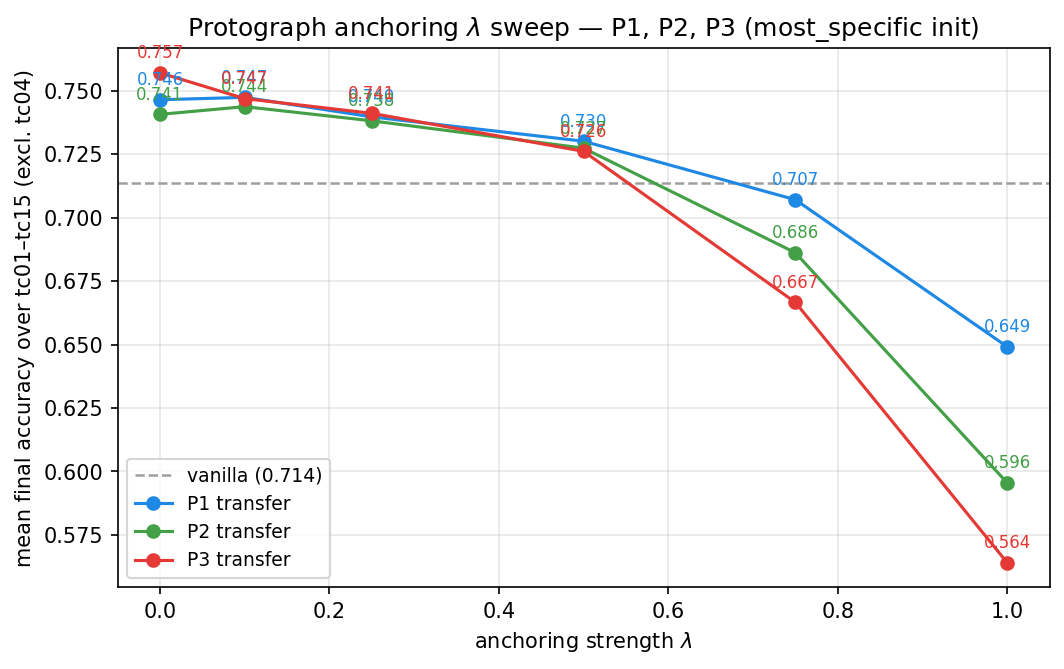
\includegraphics[width=0.72\linewidth]{assets/new_anchoring.png}
  \caption{Protograph anchoring $\lambda$ sweep: mean final LogReg test accuracy
  over the fourteen synthetic DLCC test cases (\texttt{tc01}--\texttt{tc15},
  excl.\ \texttt{tc04}) as a function of the anchoring strength $\lambda$, for the
  P1, P2 and P3 transfers (\texttt{most\_specific} initialization). Here the
  proximal pull-back is applied after \emph{every} fine-tune epoch, the last one
  included, so the saved vectors are anchored before being frozen. The
  from-scratch \texttt{vanilla} baseline is drawn as a horizontal reference. Small
  $\lambda$ leaves accuracy essentially unchanged; strong $\lambda$ degrades it
  sharply, dropping every transfer well below \texttt{vanilla} at $\lambda=1$;
  $\lambda=0$ (or a small value) is best on the mean.}
  \label{fig:anchoring_lambda_sweep}
\end{figure}

\subsection{Random Initialization Noise}
\label{sec:results_jitter}

Table~\ref{tab:jitter} and Figure~\ref{fig:jitter} report the noise ablation
of Section~\ref{sec:jitter} on tc07 and tc09--tc12 (the test cases where the
initialization carries the most signal).

\begin{table}[t]
\centering
\small
\caption{Initialization noise: change in mean final accuracy (tc07,
tc09--tc12) relative to the noise-free run of the same variant, per noise
scale $\sigma$.}
\label{tab:jitter}
\begin{tabular}{lrrrrr}
\toprule
\textbf{Variant} & $\sigma{=}0$ & $\sigma{=}0.05$ & $\sigma{=}0.1$ & $\sigma{=}0.2$ & $\sigma{=}0.5$ \\
\midrule
p1\_bound            & 0.000 & $-0.022$ & $-0.049$ & $-0.102$ & $-0.258$ \\
p2\_bound            & 0.000 & $-0.001$ & $-0.028$ & $-0.084$ & $-0.221$ \\
p3\_bound            & 0.000 & $-0.010$ & $-0.035$ & $-0.098$ & $-0.255$ \\
p1\_classic          & 0.000 & $+0.003$ & $+0.009$ & $+0.015$ & $\pm 0.000$ \\
p2\_classic          & 0.000 & $-0.019$ & $-0.037$ & $-0.071$ & $-0.108$ \\
p3\_classic          & 0.000 & $-0.027$ & $-0.042$ & $-0.085$ & $-0.114$ \\
\bottomrule
\end{tabular}
\end{table}

\begin{figure}[t]
    \centering
    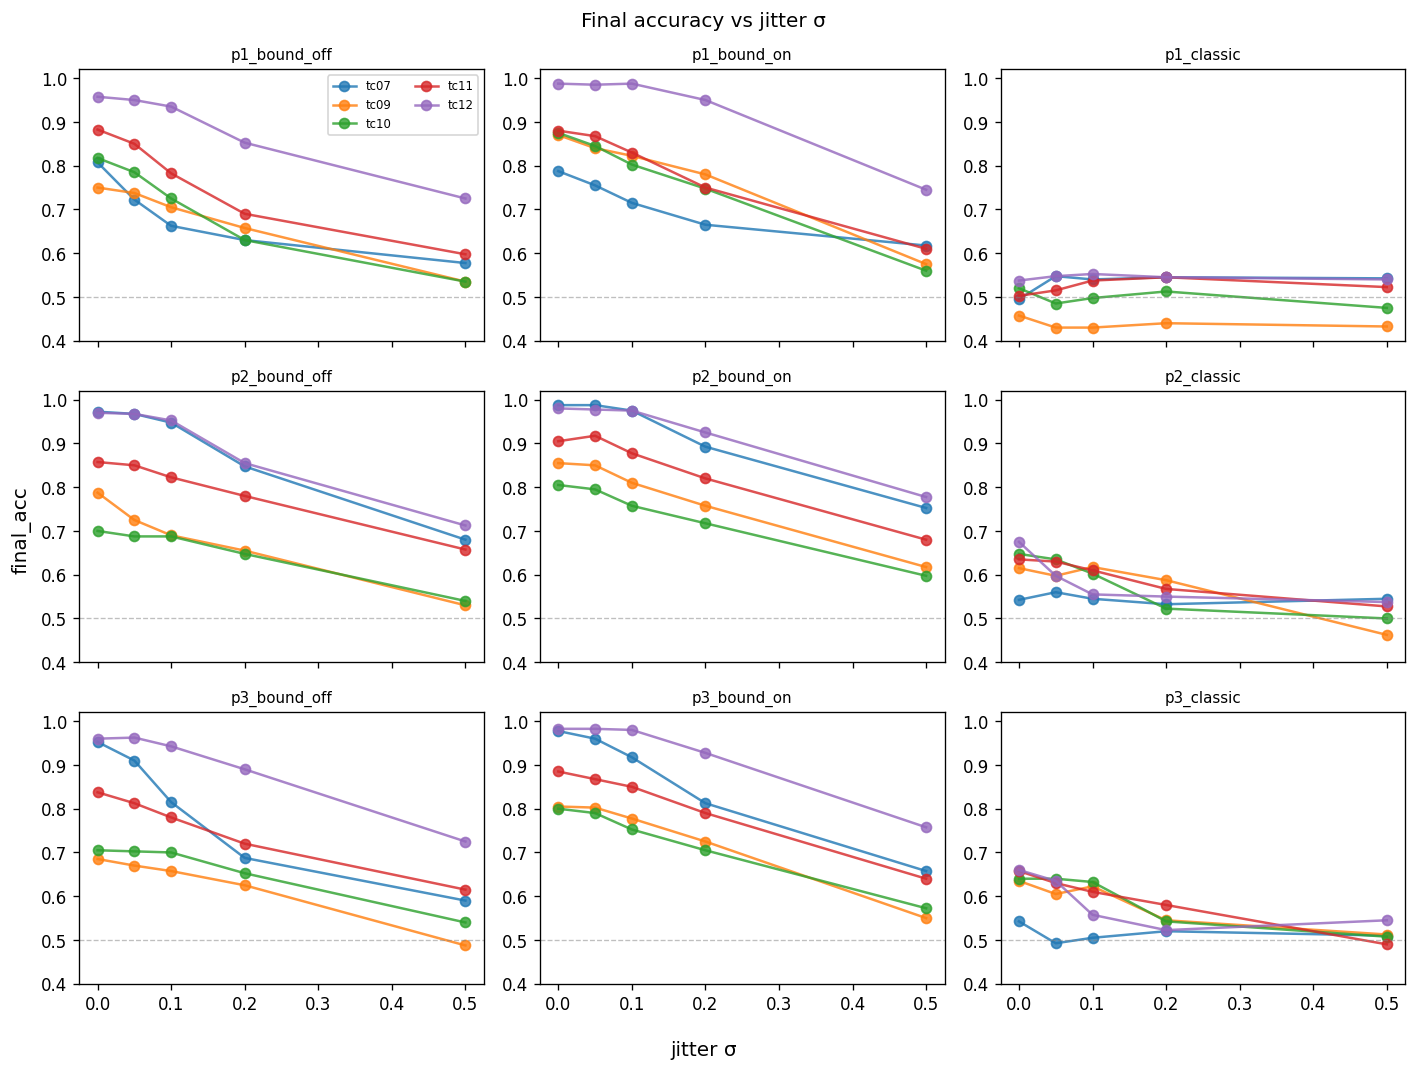
\includegraphics[width=0.8\textwidth]{assets/jitter/final_vs_sigma.png}
    \caption{Final accuracy versus initialization noise scale $\sigma$, shown
    per test case (tc07, tc09--tc12), for all six variant families.}
    \label{fig:jitter}
\end{figure}

The picture is uniform: $\sigma = 0$ is the best setting for every variant
that carries signal. The concept-bound initialization degrades smoothly with
noise (mean 0.906 $\rightarrow$ 0.685 for \texttt{p2\_bound} on the pipeline as
$\sigma$ goes from 0 to 0.5); the classic variants, which start
near chance on these test cases, are simply insensitive ($\pm$0.015 is noise
of the evaluation, not a gain: \texttt{p1\_classic} fluctuates around
0.50--0.52 at every $\sigma$). The original motivation for the noise
(Section~\ref{sec:classic_noise}), breaking ties between co-initialized
instances, is obsolete under the concept-bound construction, and as a
regularizer the noise is strictly harmful. A similar verdict holds for
anchoring toward the initialization (Section~\ref{sec:anchoring}): it provides no
reliable mean gain -- helping only on the single class-membership task
\texttt{tc14}, where the initialization is already the answer -- and degrades
accuracy at higher strength. If regularization is needed, it should target the
fine-tuning dynamics (e.g.\ the learning-rate schedule), not the
initialization or its preservation.

\subsection{Reducing Fine-Tuning Walks}
\label{sec:nw_revisited}
\label{sec:results_nw50_classic}

We shrink the instance-walk corpus from 100 to 50 and 25 walks per entity,
holding every other parameter of Section~\ref{sec:setup} fixed.
Table~\ref{tab:reduced_walks} reports the mean final accuracies and
Figure~\ref{fig:nw_bound_tc07_tc12} the per-epoch curves on the focus set.

For the classic transfer the budget is a cost lever, not an accuracy one. At
half budget the classic variants merely match full-budget \texttt{vanilla}
(0.735 and 0.726 for \texttt{p1\_classic} and \texttt{p2\_classic} against
0.721), and only on the type-centric tasks; on the relation-centric focus set
tc07--tc12 they stay in the vanilla band at every budget. At a quarter of the
corpus the saving runs out (\texttt{p2\_classic} drops to 0.667), and at equal
budget the classic transfer never beats vanilla
(Section~\ref{sec:results_synthetic}).

The concept-bound variants behave oppositely. Their epoch-0 accuracy is already
close to the final accuracy (Figure~\ref{fig:compare_epochs_tc01_tc15}), and
under the protected learning rate fine-tuning mostly \emph{erodes} the
initialization rather than building on it, so cutting walks removes drift, not
signal. On the focus set \texttt{p2\_bound} even rises as the budget shrinks
(0.917, 0.928, 0.939 at 100, 50 and 25 walks), with \texttt{p1\_bound} and
\texttt{p3\_bound} following. At a quarter budget \texttt{p2\_bound} reaches a
focus mean of 0.939 against 0.637 for full-budget \texttt{vanilla} (0.924 vs.\
0.721 over all test cases), beating it on 12 of the 14 cases while fine-tuning in
6.0\,s instead of 21.9\,s, a 3.6$\times$ saving on the stage that dominates
runtime (Section~\ref{sec:results_runtime}).

Full-budget \texttt{vanilla} stays ahead on only two cases, tc03 (0.945 vs.\
0.807) and tc06 (0.983 vs.\ 0.932), where the discriminating signal is
irreducibly instance-level, a particular (subject, relation) pair or undirected
participation in a relation, and no schema initialization can substitute for the
walks. The budget can be cut where the schema carries the signal; where it does
not, the walks remain the carrier and their budget the price.

\begin{table}[t]
\centering
\small
\caption{Mean final test accuracy (after 5 fine-tuning epochs) under shrinking
instance-walk budgets, averaged over all 14 comparison test cases
(tc01--tc15 without tc04). All variants share the same walk corpus per budget;
the protograph walk budget is unchanged.}
\label{tab:reduced_walks}
% Auto-generated by scripts/plot_reduced_walks.py
\begin{tabular}{lccc}
\toprule
\textbf{Variant} & 100 walks (full) & 50 walks & 25 walks \\
\midrule
\texttt{vanilla} & 0.721 & 0.709 & 0.699 \\
\texttt{p1\_classic} & 0.740 & 0.735 & 0.722 \\
\texttt{p2\_classic} & 0.741 & 0.726 & 0.667 \\
\texttt{p3\_classic} & 0.734 & 0.681 & 0.618 \\
\texttt{p1\_bound} & 0.881 & 0.892 & 0.885 \\
\texttt{p2\_bound} & 0.912 & 0.922 & 0.924 \\
\texttt{p3\_bound} & 0.908 & 0.912 & 0.904 \\
\bottomrule
\end{tabular}

\end{table}

\begin{figure}[p]
  \centering

  % Row 1
  \begin{subfigure}[t]{0.46\textwidth}
      \centering
      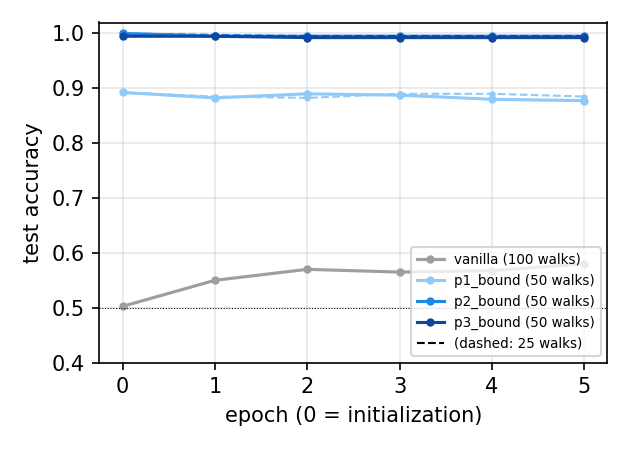
\includegraphics[width=\linewidth]{assets/nw_bound/tc07_nwbound.png}
      \caption{TC07}
  \end{subfigure}
  \hfill
  \begin{subfigure}[t]{0.46\textwidth}
      \centering
      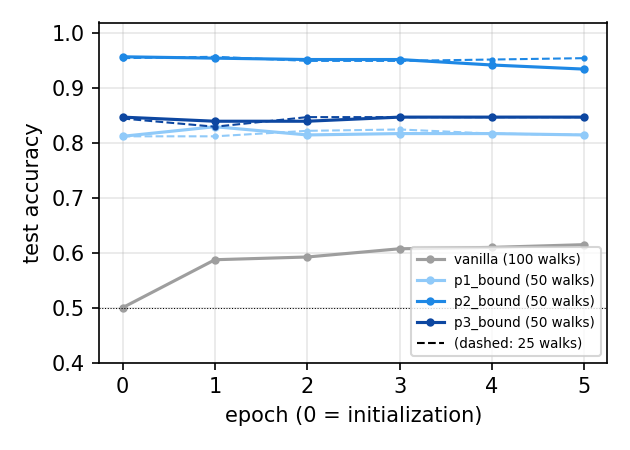
\includegraphics[width=\linewidth]{assets/nw_bound/tc08_nwbound.png}
      \caption{TC08}
  \end{subfigure}

  \vspace{0.6em}

  % Row 2
  \begin{subfigure}[t]{0.46\textwidth}
      \centering
      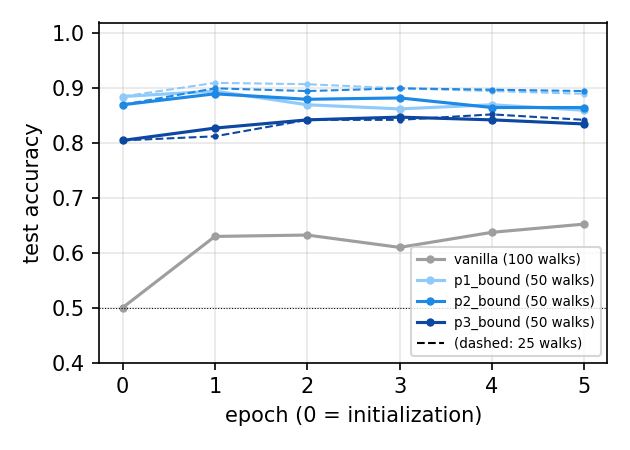
\includegraphics[width=\linewidth]{assets/nw_bound/tc09_nwbound.png}
      \caption{TC09}
  \end{subfigure}
  \hfill
  \begin{subfigure}[t]{0.46\textwidth}
      \centering
      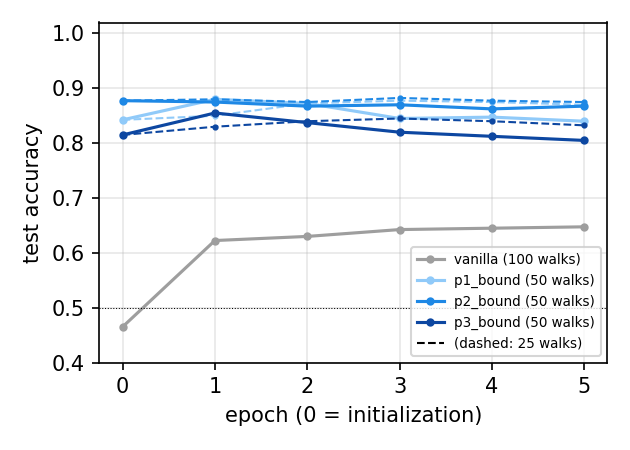
\includegraphics[width=\linewidth]{assets/nw_bound/tc10_nwbound.png}
      \caption{TC10}
  \end{subfigure}

  \vspace{0.6em}

  % Row 3
  \begin{subfigure}[t]{0.46\textwidth}
      \centering
      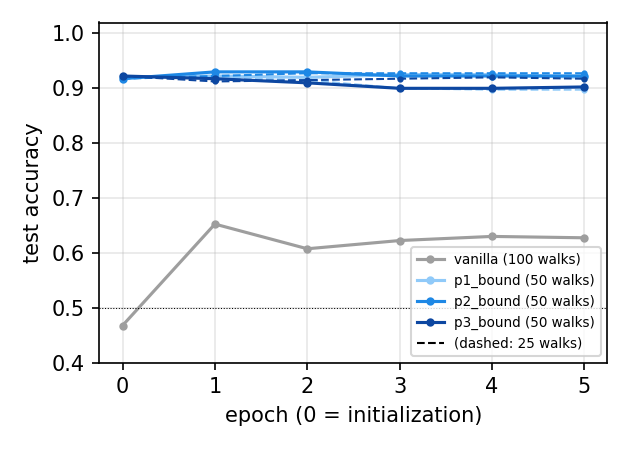
\includegraphics[width=\linewidth]{assets/nw_bound/tc11_nwbound.png}
      \caption{TC11}
  \end{subfigure}
  \hfill
  \begin{subfigure}[t]{0.46\textwidth}
      \centering
      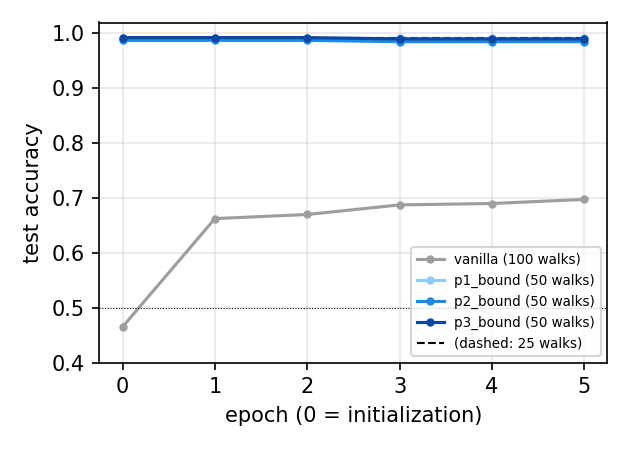
\includegraphics[width=\linewidth]{assets/nw_bound/tc12_nwbound.png}
      \caption{TC12}
  \end{subfigure}

  \caption{Per-epoch test accuracy on the relation-centric focus test cases
  under reduced fine-tuning walk budgets. Gray: \texttt{vanilla} on the full
  corpus (100 walks per entity). Blue: the concept-bound variants fine-tuned
  on half the corpus (50 walks per entity, solid) and a quarter of the corpus
  (25 walks per entity, dashed).}
  \label{fig:nw_bound_tc07_tc12}
\end{figure}

\subsection{Direction-Aware Cardinality}
\label{sec:results_direction}

We ablate the direction tag of Section~\ref{sec:cardinality} on the test-case
pairs whose labels depend on edge direction: tc01/tc02 (the existence-only
control, $\exists r.\top$ vs.\ $\exists r^{-}.\top$) and the cardinality pairs
tc09/tc10 and tc11/tc12. The ablation proceeds in three steps of increasing
realism: (i) an exact-count \emph{oracle} that measures how much label
information edge direction carries in principle, (ii) a probe on the raw
initialization vectors, and (iii) the full fine-tuning pipeline. This paragraph
covers the oracle; the probe and pipeline follow below.

\paragraph{Oracle.} The oracle bypasses the embedding entirely and works
directly from ground-truth graph structure, so it reports the best any
classifier could do. For each labeled entity we count its exact out-degree and
in-degree per relation, and train a logistic regression under two feature
encodings: \emph{undirected}, where out- and in-counts are summed into one
count per relation (direction discarded), and \emph{directed}, where they are
kept as two separate features (direction preserved). Alongside accuracy we
report the \emph{Bayes error} of the target-relation count feature -- the
lowest error rate any classifier could achieve on that feature. It is nonzero
exactly when entities of opposite labels share the same feature value and are
therefore impossible to tell apart from that feature alone. We compute it to
separate two failure modes: a nonzero Bayes error means positives and negatives
have become genuinely indistinguishable once direction is collapsed, so no
classifier of any kind can recover them; a zero Bayes error paired with low
accuracy means the labels are still perfectly determined by the features but the
classes are no longer \emph{linearly} separable -- a limitation of the linear
probe, not a loss of information.
Table~\ref{tab:direction_oracle} shows that the directed encoding solves all
six test cases perfectly (LogReg accuracy $1.000$, Bayes error $0.000$).
Discarding direction is harmless on tc11/tc12 but costly elsewhere, removing up
to $14.5$ accuracy points (tc10). The sharpest failure is tc01: the information
is still technically present (Bayes error $0.000$), yet logistic regression
collapses to $0.560$, barely above chance. The summed encoding is \emph{linearly
inseparable} here because a few negative hub entities have so many incoming
target-relation edges that their summed count exceeds that of the positives, so
the optimal decision boundary in the collapsed channel would have to be
non-monotone -- something a linear classifier cannot represent.

\begin{table}[t]
\centering
\small
\caption{Exact-count oracle on the directional test cases. Bayes error of the
target-relation count feature (lower is better) and LogReg test accuracy on
exact count features over all relations (higher is better), with direction
collapsed (undir.) vs.\ separated (dir.).}
\label{tab:direction_oracle}
\begin{tabular}{lcccc}
\toprule
\textbf{TC} & \textbf{Bayes err.\ undir.} & \textbf{Bayes err.\ dir.} & \textbf{LogReg undir.} & \textbf{LogReg dir.} \\
\midrule
tc01 & 0.000 & 0.000 & 0.560 & 1.000 \\
tc02 & 0.017 & 0.000 & 0.955 & 1.000 \\
tc09 & 0.048 & 0.000 & 0.888 & 1.000 \\
tc10 & 0.112 & 0.000 & 0.855 & 1.000 \\
tc11 & 0.000 & 0.000 & 1.000 & 1.000 \\
tc12 & 0.000 & 0.000 & 1.000 & 1.000 \\
\bottomrule
\end{tabular}
\end{table}

\paragraph{Init-space probe and full pipeline.}
Table~\ref{tab:direction_pipeline} reports the end-to-end result on the
cardinality test cases: final accuracy after 5 protected fine-tuning epochs.
The baseline column is the concept-bound initialization \emph{without} the
cardinality count term ($\delta{=}0$, direction-blind binding); the four tagged
columns add that count term back and vary only the direction tag on the
incoming-edge code, so the table reads left to right as the marginal effect of
the count term and of tagging its direction.
Figure~\ref{fig:direction_tags} shows the corresponding probe accuracies and
epoch curves.

\begin{table}[t]
\centering
\small
\caption{Direction-tag ablation on the cardinality test cases, full pipeline:
final test accuracy after 5 protected fine-tuning epochs (P2 protograph
initialization). The baseline \textbf{no card.} is the concept-bound
initialization \emph{without} the cardinality count term ($\delta{=}0$,
direction-blind binding); \texttt{shared}/\texttt{rolled}/\texttt{negated}/%
\texttt{keyed} add that count term back with the corresponding direction tag on
the incoming-edge code. \texttt{rolled} is the default tag. Best per row in
bold. The same comparison averaged over the P1/P2/P3 initializations and across
all six directional test cases is given in Appendix~\ref{app:direction-all}.}
\label{tab:direction_pipeline}
\begin{tabular}{lccccc}
\toprule
\textbf{TC} & \textbf{no card.} & \textbf{shared} & \textbf{rolled} & \textbf{negated} & \textbf{keyed} \\
\midrule
tc09 & 0.778 & 0.758 & 0.870 & 0.815 & \textbf{0.890} \\
tc10 & 0.742 & 0.725 & \textbf{0.868} & 0.730 & 0.812 \\
tc11 & 0.880 & 0.888 & 0.922 & 0.832 & \textbf{0.930} \\
tc12 & 0.980 & 0.980 & \textbf{0.988} & 0.952 & 0.978 \\
\midrule
Mean & 0.845 & 0.838 & \textbf{0.912} & 0.832 & 0.903 \\
\bottomrule
\end{tabular}
\end{table}

\begin{figure}[t]
    \centering
    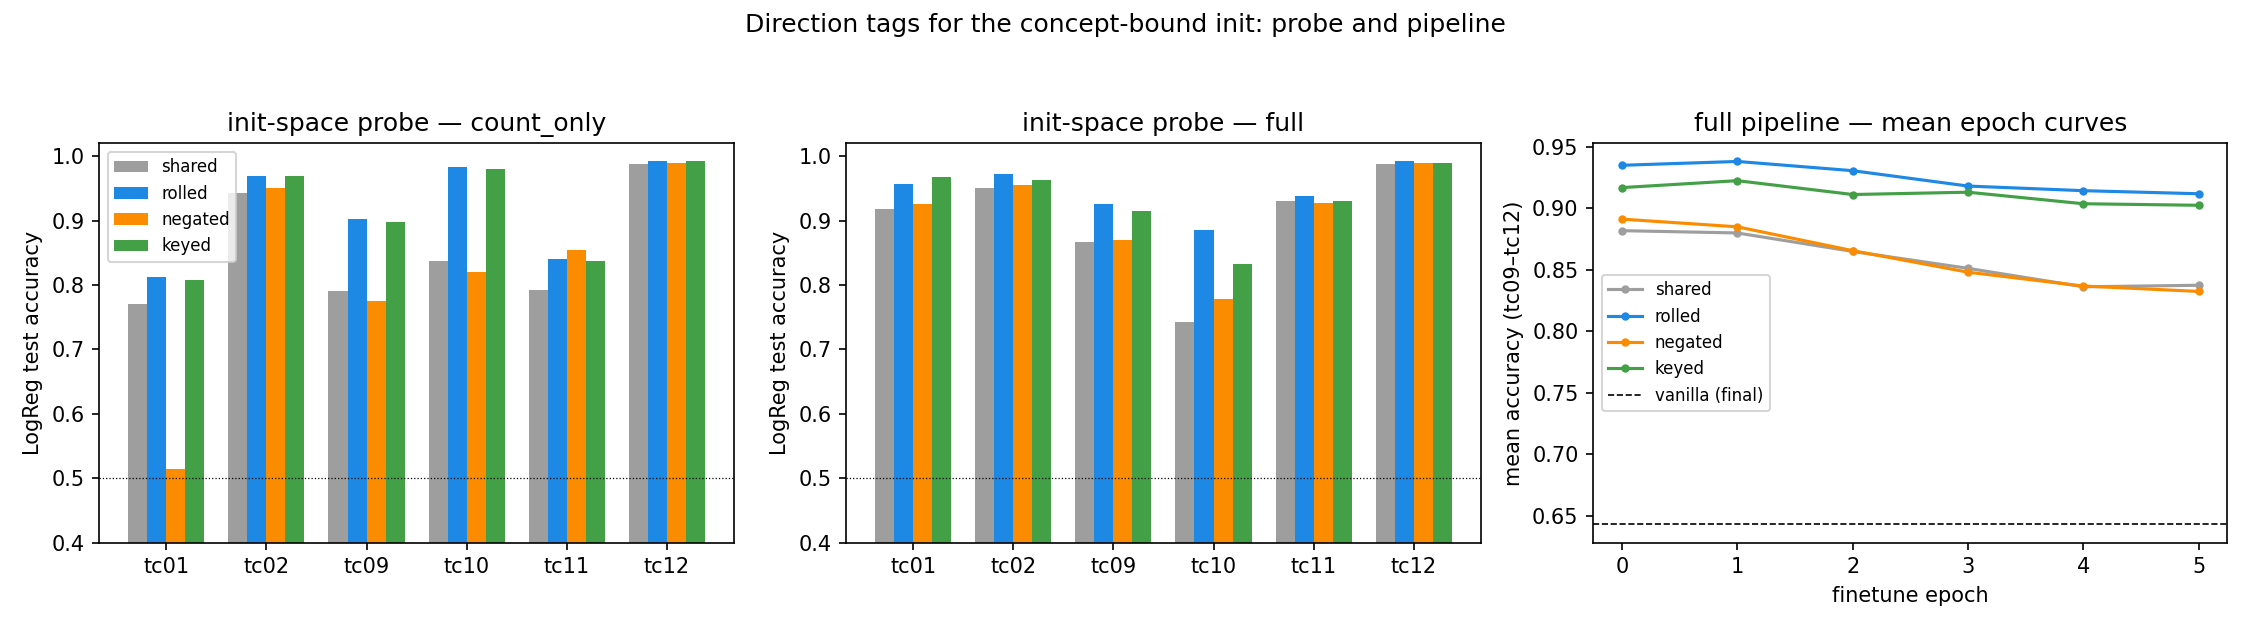
\includegraphics[width=\textwidth]{assets/direction/direction_tag_comparison.png}
    \caption{Direction tags for the concept-bound initialization: LogReg
    probes directly on the initialization vectors (left: cardinality channel
    isolated, $\alpha{=}\beta{=}\gamma{=}0$; middle: full recipe) and mean
    epoch curves of the full pipeline on tc09--tc12 (right).}
    \label{fig:direction_tags}
\end{figure}


Three conclusions follow. First, \emph{direction is real, label-relevant
information, and a direction-blind count term loses it}: adding the count term
\emph{without} a direction tag (\texttt{shared}, mean 0.838) does not improve on
the count-free baseline (\texttt{no card.}, 0.845) at all, whereas tagging the
direction of that same count term (\texttt{rolled}) lifts the mean to 0.912 -- 
a 7.4-point gain (0.838 $\rightarrow$ 0.912) and up to 14 points on tc10, the
inverse-cardinality task. The protected fine-tuning cannot repair a
direction-blind initialization, exactly as the oracle predicted. Second,
\emph{the roll operation is nothing special}: a fixed random $\pm 1$ key
(\texttt{keyed}) performs on par (mean 0.903), confirming that any fixed,
norm-preserving, decorrelating transform gives incoming counts their own
quasi-orthogonal channel; $\mathrm{roll}$ is simply the cheapest such
transform. Third, \emph{negation is a direction tag that fails differently}:
$-\mathrm{emb}(r)$ encodes $\text{out} - \text{in}$ in a single channel and
lands at the direction-blind level overall (0.832), collapsing to chance on
the tc01 count-only probe where positives and in-edge hubs cancel.

Interestingly, the oracle also shows that tc11/tc12 do \emph{not} require the
direction tag at the information level (undirected Bayes error is zero); the
small but consistent wins of the tagged variants there are a geometry effect,
not an information effect.

\section{Results on DBpedia}
\label{sec:results_dbpedia}

Finally, we port the comparison to the real DBpedia graph and the DLCC DBpedia
gold standard. The DBpedia graph is the English DBpedia Snapshot 2021-09
release~\cite{dbpedia_snapshot_2021}, from which we materialize an instance graph
of roughly 29 million IRI triples by combining the mapping-based object
properties with the most-specific instance types. The headline comparison
(Section~\ref{sec:dbpedia_headline})
establishes a puzzle: the concept-bound construction is the best
\emph{initialization} on a real, noisy schema, yet it loses end-to-end.
Section~\ref{sec:dbpedia_diagnosis} traces this puzzle to three stacked
mechanisms of the real corpus and benchmark. The remaining subsections evaluate
the family of remedies those mechanisms motivate. We tame the initialization's
pathological norm tail with a per-row cap (Section~\ref{sec:dbpedia_cap}) or by
compressing counts at construction time (Section~\ref{sec:dbpedia_compress}). We
reshape the class-mean term with specificity weighting
(Section~\ref{sec:dbpedia_specificity}) and the asserted hierarchy with decay or
most-specific weighting (Section~\ref{sec:dbpedia_hierarchy}). Finally, the
cap-size and learning-rate ablations pin down the design points
(Section~\ref{sec:dbpedia_ablations}).

\begin{figure}[t]
    \centering
    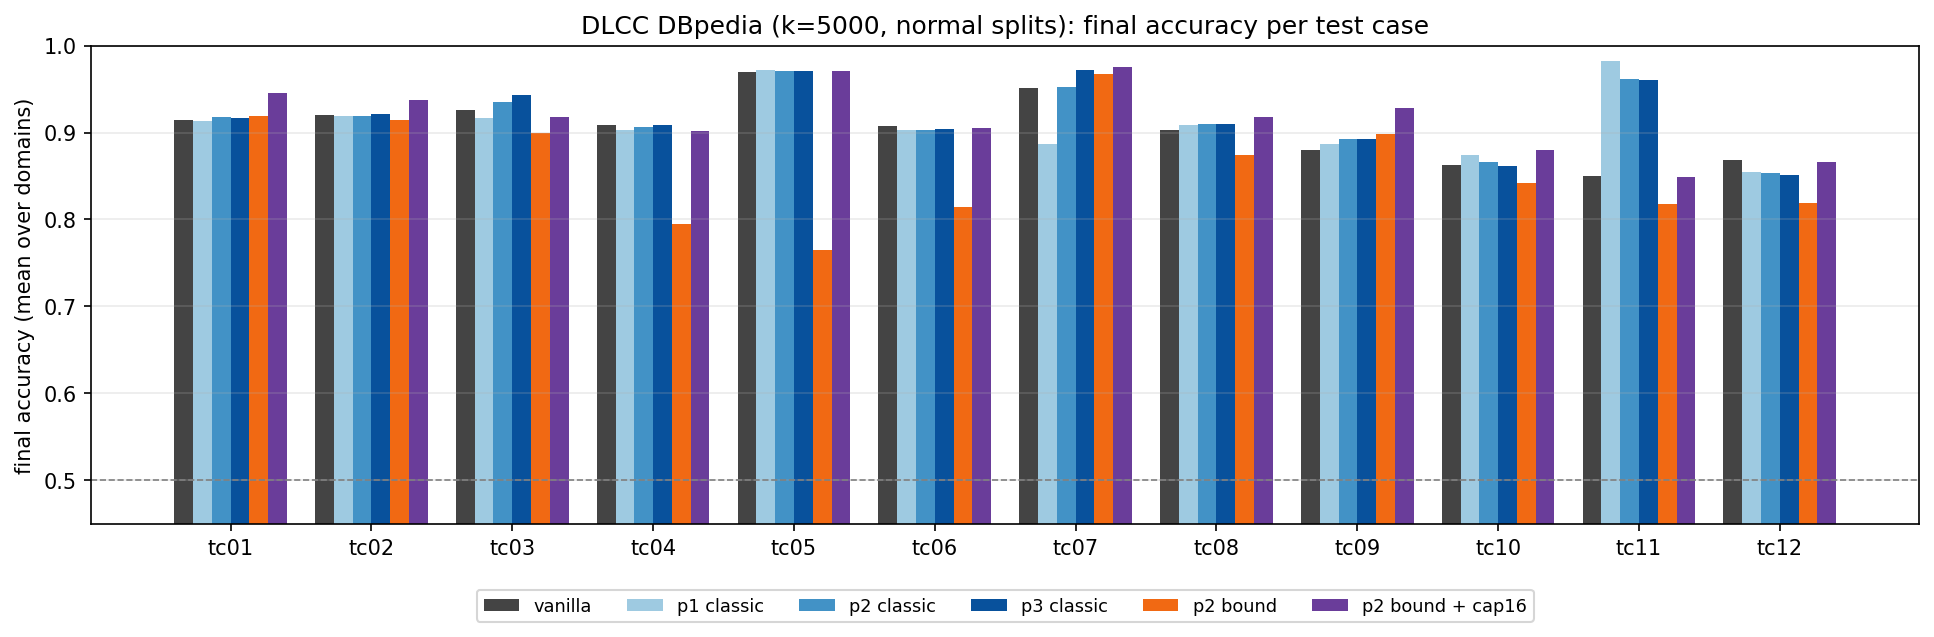
\includegraphics[width=\textwidth]{assets/dbpedia/final_acc.png}
    \caption{Final test accuracy per test case (mean over domains, regular
    splits) on the full $1.16$B-token corpus and the raw lens, for
    \texttt{vanilla}, the three classic variants and \texttt{p2\_bound}, together
    with the capped bound init (\texttt{p2 bound + cap16}). The five shared
    columns reproduce Table~\ref{tab:dbpedia_per_tc}. The cap restores tc04--tc06 and tc11/tc12,
    where the un-capped \texttt{p2\_bound} drops well below \texttt{vanilla},
    while keeping the bound's lead on tc07 and tc09.}
    \label{fig:dbpedia6_final}
\end{figure}

\subsection{Headline Comparison}
\label{sec:dbpedia_headline}

We compare vanilla, classic, and bound variants on P1, P2, and P3 embeddings
over 89 splits
(tc01--tc12 $\times$ six domains, regular and hard variants, $k = 5000$).
Table~\ref{tab:dbpedia_per_tc} breaks the final accuracy down by test case and
split difficulty (regular vs.\ hard), and
Figure~\ref{fig:dbpedia_epochs} shows the per-epoch behavior.

\paragraph{Removing the universal class \texttt{owl:Thing}.} The root of
DBpedia's class hierarchy is \texttt{owl:Thing}~\cite{owl2_overview_2012}, the
class every entity belongs to by definition. We delete it before building any protograph or initialization:
a class shared by every entity carries no distinguishing signal, and keeping it
would make it a hub linked to all classes and entities, whose dominant embedding
would drown out the specific class signal we want to transfer. Concretely, we
keep only the classes DBpedia declares as \texttt{rdf:type owl:Class} and drop
every \texttt{rdfs:subClassOf} and \texttt{rdf:type} edge pointing to
\texttt{owl:Thing}.

\begin{table}[t]
\centering
\small
\caption{DLCC DBpedia gold standard: final test accuracy (after 5 fine-tuning
epochs) averaged over domains, separately for the regular and hard splits of
each test case (\texttt{\_hard}). The best variant per row is in bold. The final
row is the overall mean over all 89 splits.}
\label{tab:dbpedia_per_tc}
\footnotesize
\setlength{\tabcolsep}{3.5pt}
\begin{tabular}{lccccccc}
\toprule
\textbf{Test case} & \textbf{vanilla} & \textbf{p1\_classic}
& \textbf{p2\_classic} & \textbf{p3\_classic} & \textbf{p1\_bound}
& \textbf{p2\_bound} & \textbf{p3\_bound} \\
\midrule
tc01 & 0.915 & 0.913 & 0.918 & 0.917 & 0.911 & \textbf{0.919} & 0.914 \\
tc01\_hard & 0.673 & 0.656 & 0.688 & 0.687 & \textbf{0.761} & 0.758 & 0.756 \\
tc02 & 0.920 & 0.919 & 0.919 & \textbf{0.921} & 0.805 & 0.915 & 0.917 \\
tc02\_hard & 0.640 & 0.676 & 0.675 & 0.656 & 0.695 & 0.698 & \textbf{0.701} \\
tc03 & 0.926 & 0.916 & 0.935 & \textbf{0.943} & 0.893 & 0.900 & 0.889 \\
tc04 & \textbf{0.909} & 0.903 & 0.906 & 0.908 & 0.807 & 0.795 & 0.804 \\
tc04\_hard & 0.913 & 0.914 & 0.911 & \textbf{0.916} & 0.773 & 0.770 & 0.769 \\
tc05 & 0.969 & \textbf{0.972} & 0.971 & 0.971 & 0.732 & 0.765 & 0.810 \\
tc06 & \textbf{0.908} & 0.903 & 0.903 & 0.904 & 0.826 & 0.815 & 0.814 \\
tc06\_hard & 0.852 & \textbf{0.880} & \textbf{0.880} & 0.872 & 0.729 & 0.779 & 0.733 \\
tc07 & 0.951 & 0.887 & 0.953 & \textbf{0.971} & 0.958 & 0.968 & 0.963 \\
tc08 & 0.902 & 0.908 & 0.909 & \textbf{0.910} & 0.839 & 0.874 & 0.864 \\
tc09 & 0.880 & 0.886 & 0.893 & 0.892 & 0.889 & \textbf{0.898} & 0.890 \\
tc09\_hard & 0.774 & 0.796 & 0.799 & 0.800 & 0.819 & \textbf{0.837} & 0.825 \\
tc10 & 0.863 & \textbf{0.874} & 0.866 & 0.862 & 0.842 & 0.841 & 0.844 \\
tc10\_hard & 0.652 & 0.659 & 0.664 & 0.659 & 0.677 & \textbf{0.679} & 0.674 \\
tc11 & 0.850 & \textbf{0.983} & 0.961 & 0.961 & 0.906 & 0.818 & 0.794 \\
tc11\_hard & 0.704 & \textbf{0.739} & 0.709 & 0.639 & 0.686 & 0.661 & 0.618 \\
tc12 & \textbf{0.868} & 0.854 & 0.854 & 0.851 & 0.823 & 0.818 & 0.821 \\
tc12\_hard & 0.669 & 0.656 & \textbf{0.679} & 0.672 & 0.664 & 0.676 & 0.648 \\
\midrule
\textbf{All (89)} & 0.831 & 0.843 & \textbf{0.844} & 0.839 & 0.799 & 0.803 & 0.797 \\
\bottomrule
\end{tabular}
\end{table}

\begin{figure}[t]
    \centering
    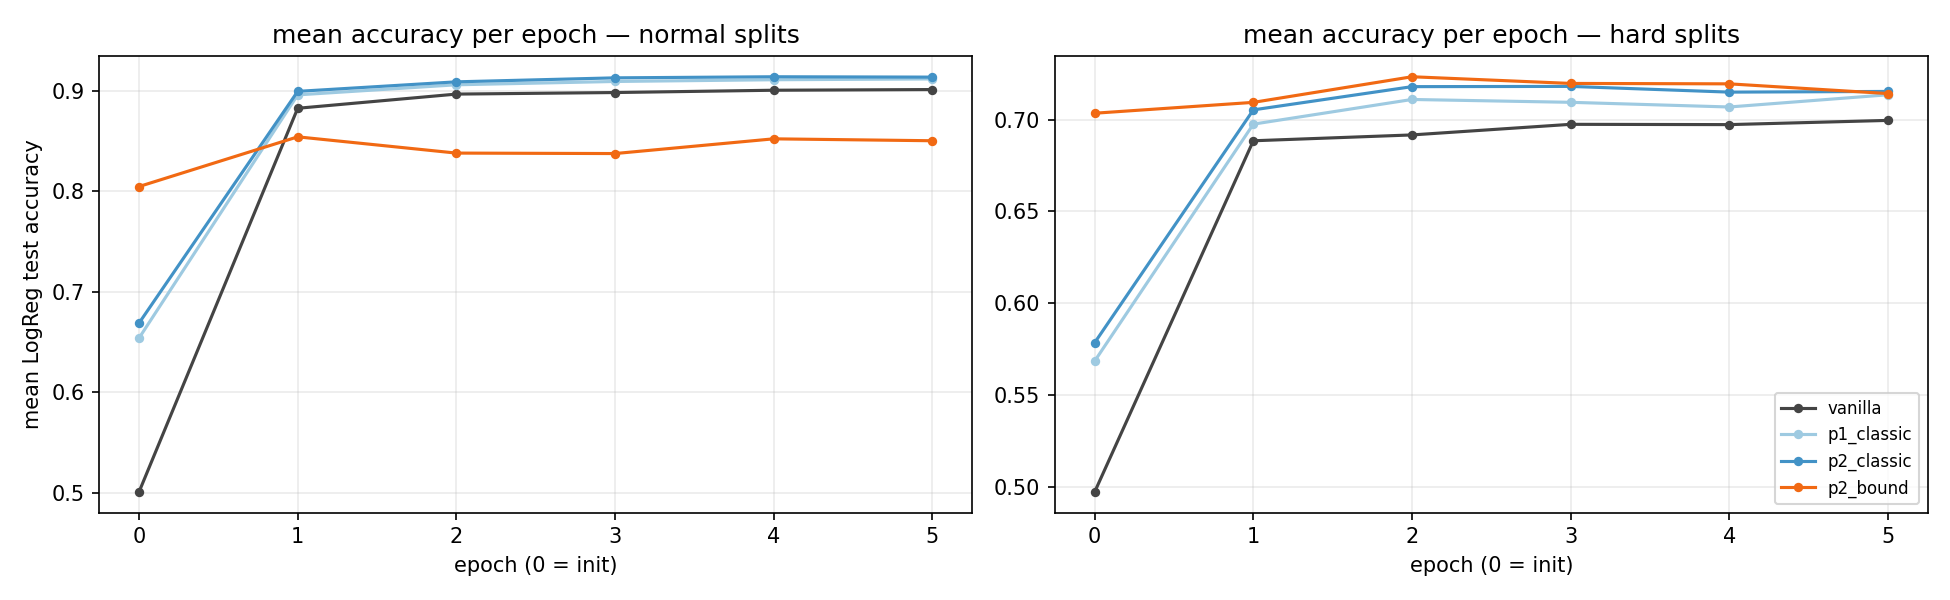
\includegraphics[width=\textwidth]{assets/dbpedia/acc_per_epoch.png}
    \caption{Test accuracy per fine-tuning epoch on the DBpedia gold standard,
    for the regular (left) and hard (right) splits (mean over the 89 splits);
    epoch~0 is the initialization. The bound variants start far above all
    others; on the regular splits the classic transfers overtake them within the
    first epoch, while on the hard splits the bound init stays competitive
    throughout.}
    \label{fig:dbpedia_epochs}
\end{figure}

The real-graph picture is more nuanced than the synthetic one.

\textbf{The bound initialization transfers.} At epoch 0, every bound variant
already reaches $\approx 0.76$--$0.77$ mean accuracy (\texttt{p2\_bound} 0.769,
\texttt{p3\_bound} 0.764), against 0.500 for the untrained vanilla model and
0.638 for the classic transfer. The construction works on a real, noisy schema:
one-hop schema features are linearly readable before any instance training.

\textbf{End-to-end, the classic transfer wins on the overall mean.} After 5
epochs, \texttt{p2\_classic} leads on the overall mean (0.844/0.916/0.751) with
\texttt{p3\_classic} marginally ahead on the regular splits (0.918) but behind
overall (0.839); the bound variants trail (0.803). The per-test-case breakdown
in Table~\ref{tab:dbpedia_per_tc} shows this is not uniform: \texttt{p2\_bound}
\emph{wins} on the hard splits of the existence and cardinality families (e.g.\
tc01-hard 0.758 vs.\ 0.673, tc09-hard 0.837 vs.\ 0.774, tc10-hard 0.679 vs.\
0.652 against vanilla), exactly the constructors the synthetic analysis
predicts. The loss is concentrated on tc04--tc06, the families built around
\emph{enumerated individuals} ($\{e\}$ constructors): there the label depends on
instance-specific information that no schema feature can carry, the rich
DBpedia walk corpus contains the needed signal, and the uniformly
\emph{protected} learning rate prevents the bound models from learning it
(tc05: 0.765 vs.\ 0.969 for vanilla).

\textbf{The protograph level is not the bottleneck.} P3 was the decisive upgrade
on the synthetic leaf-typed graphs, but on DBpedia \texttt{p3\_bound}
($0.797$/$0.860$/$0.716$) is indistinguishable from \texttt{p2\_bound}, and
\texttt{p3\_classic} only edges \texttt{p2\_classic} on the regular splits while
losing on the hard ones. DBpedia's specific-type dump plus ancestor
materialization already gives nearly every class lookup a pretrained code under
P2, so the extra P3 leaf codes add little; the binding construction and the
fine-tuning policy, not the protograph depth, decide the outcome here.

The concept-bound construction is therefore validated as an
\emph{initialization} method on a real, noisy graph; the open question is why a
state-of-the-art initializer loses end-to-end, and whether the construction or
the fine-tuning policy is to blame. The next subsection isolates the cause; the
ones after it evaluate the remedies.

\subsection{Why the Synthetic Gains Do Not Transfer}
\label{sec:dbpedia_diagnosis}

On the synthetic suite the bound construction was worth $+20$ to $+40$ points
end-to-end on the qualified-existential and cardinality families; on DBpedia the
same families yield at most a few points, and the overall mean falls behind both
classic and vanilla. The init is not broken: at epoch~0 it is as dominant here
as on the synthetic graphs (0.769 vs vanilla's chance-level 0.500). We did not
run a controlled ablation that isolates each cause on the real graph, so what
follows is a diagnosis rather than a decomposition. Three properties of the
\emph{real corpus and benchmark}, rather than of the construction, most
plausibly account for why the end-to-end gap closes, and we read them as acting
together.

\paragraph{1. There is little headroom.}
The synthetic generator deliberately decorrelates each constructor from degree,
popularity, and class, so vanilla skip-gram plateaus at $0.58$--$0.67$ on
tc07--tc12 and a better initialization has $\approx 0.37$ of headroom to claim.
On the real graph nothing is decorrelated, and the 1.16B-token walk corpus
($\approx 900$ occurrences per vocabulary word per epoch) lets vanilla absorb
all of it: its mean accuracy jumps $0.50 \rightarrow 0.815$ within the
\emph{first} epoch -- 98\% of its final $0.831$ (Figure~\ref{fig:dbpedia_epochs})
 -- and the tc07--tc12 families it once struggled with are already solved to
$0.886$ on the regular splits. A second reason vanilla closes the gap is that,
unlike the synthetic graph, the DBpedia instance graph carries explicit
$\mathit{rdf{:}type}$ assertions, and the random walks traverse them. Every
entity's class memberships therefore appear directly in the walk corpus, so
vanilla skip-gram learns them as ordinary co-occurrences. The ontology signal
that the concept-bound init injects by hand is already present in the training
data, and vanilla absorbs it for free: the corpus implicitly leaks the schema
information that gave the init its edge on the synthetic suite, whose walks never
expose type membership this way. That leaves $\approx 0.11$ of headroom where the
synthetic suite offered $0.37$. Vanilla learns the schema only
\emph{approximately} from co-occurrence, so a class-mean start that places every
entity exactly at its class code still sharpens this geometry; this is the narrow
residual on which the classic transfer edges vanilla end-to-end ($0.844$ vs.\
$0.831$), a gap only just above the ${\approx}0.003$ DBpedia run-to-run noise.

\paragraph{2. The benchmark mass on a real graph is degree-shaped.}
Most of that baseline strength is not constructor understanding but
degree/popularity signal that every corpus-trained model absorbs for free. A
Logistic Regression on four trivial per-entity statistics -- $\log$ out-degree,
$\log$ in-degree, and the number of distinct outgoing and incoming predicates,
with \emph{no embeddings at all} -- scores $0.791$ on the regular splits and
$0.739$ on the hard ones (Table~\ref{tab:dbpedia_degree_probe}), the latter
\emph{above} fully trained vanilla's $0.700$. On a real KG the constructors
cannot be decorrelated from degree the way the synthetic generator did: $\geq 2r$
literally implies a higher degree, and popular entities carry most relations. The
schema-bound channels can therefore only add at the margin above this probe -- 
which they do, exactly on the hard existence and cardinality splits the
direction-tagged count term targets (tc01-hard, tc02-hard, tc09-hard).

\begin{table}[t]
\centering
\small
\caption{A degree-only probe versus fully trained \texttt{vanilla} (final
per-split mean accuracy, averaged over domains). The probe is a Logistic
Regression on four statistics per entity -- $\log$ out/in-degree and the number of
distinct outgoing/incoming predicates ($\mathit{rdf{:}type}$ excluded) -- with no
embeddings. Probe cells that match or beat trained \texttt{vanilla} are in bold.
On the hard splits the four degree numbers are on average \emph{not} beaten by
trained \texttt{vanilla} ($0.739$ vs $0.700$).}
\label{tab:dbpedia_degree_probe}
\begin{tabular}{lcc}
\toprule
\textbf{Test case} & \textbf{degree probe} & \textbf{vanilla} \\
\midrule
tc01       & 0.778 & 0.915 \\
tc01\_hard & \textbf{0.689} & 0.673 \\
tc02       & 0.897 & 0.920 \\
tc02\_hard & \textbf{0.749} & 0.640 \\
tc03       & 0.772 & 0.926 \\
tc04       & 0.611 & 0.909 \\
tc04\_hard & 0.547 & 0.913 \\
tc05       & 0.643 & 0.969 \\
tc06       & 0.641 & 0.908 \\
tc06\_hard & 0.581 & 0.852 \\
tc07       & 0.705 & 0.951 \\
tc08       & \textbf{0.930} & 0.902 \\
tc09       & 0.842 & 0.880 \\
tc09\_hard & \textbf{0.790} & 0.774 \\
tc10       & \textbf{0.967} & 0.863 \\
tc10\_hard & \textbf{0.822} & 0.652 \\
tc11       & 0.733 & 0.850 \\
tc11\_hard & 0.620 & 0.704 \\
tc12       & \textbf{0.944} & 0.868 \\
tc12\_hard & \textbf{0.801} & 0.669 \\
\midrule
\textbf{Overall (regular)} & 0.791 & 0.901 \\
\textbf{Overall (hard)}    & \textbf{0.739} & 0.700 \\
\bottomrule
\end{tabular}
\end{table}

\paragraph{3. The protected fine-tune freezes the bound model's hub rows.}
The concept-bound init accumulates one unit vector per (edge, neighbour-class)
pair plus direction-tagged relation counts, then receives a single
\emph{global} rescale (mean norm $\rightarrow 8$). A few high-degree entities
accumulate far more counts than the rest, so the rescale leaves a small set of
\emph{hub} rows with pathologically large norms: the median row sits at
$\approx 1.8$ while the maximum reaches $\approx 65{,}000$
(Table~\ref{tab:dbpedia_norms}). A fixed-size gradient step barely turns a vector
that long, so at the protected rate $0.0025$ it is precisely these hub rows that
fail to move: after five epochs the tail is essentially the init's
(p99.9 drops only $594 \rightarrow 498$, the maximum stays $\approx 64{,}000$),
while vanilla's rows sit in a tight band (max $17.7$). Freezing the hubs is what
\emph{preserves} the tc07/tc09 constructor wins, but it equally blocks the
recovery vanilla gets on tc04--tc06, the families built around enumerated
individuals ($\{e\}$ constructors): there the label depends on instance-specific
information no schema feature can carry, the corpus contains it, and the frozen
hub rows cannot learn it (tc05 $0.765$ vs vanilla $0.969$). That single family
costs the bound mean more than all its constructor-matched wins add.

\begin{table}[t]
\centering
\small
\caption{Entity-row L2-norm distribution. The concept-bound init's heavy tail
(p99--max) is created at construction time and is essentially \emph{unchanged}
after five protected fine-tuning epochs -- the hub rows are frozen -- whereas
\texttt{vanilla} keeps all rows in a tight band. This is the mechanism the
per-row cap and the build-time count compression of the following subsections
remove.}
\label{tab:dbpedia_norms}
\begin{tabular}{lccccc}
\toprule
\textbf{Embedding} & \textbf{median} & \textbf{p90} & \textbf{p99} & \textbf{p99.9} & \textbf{max} \\
\midrule
\texttt{vanilla} (final)        & 2.58 & 5.36  & 7.21  & 8.71  & 17.7 \\
\texttt{p2\_bound} (init)       & 1.80 & 10.64 & 67.58 & 594.3 & 65339 \\
\texttt{p2\_bound} (final)      & 2.97 & 15.59 & 75.80 & 498.0 & 64081 \\
\bottomrule
\end{tabular}
\end{table}

None of the three points to ``the init stopped working.'' The construction
remains the best initializer on a real, noisy schema, and the end-to-end deficit
looks less like a flaw in the construction than like a \emph{policy} problem: the
count-accumulating norm tail left untouched under a uniformly protected learning
rate. The remaining subsections tame that tail (per-row cap;
build-time compression), reshape the init's class content (specificity and
hierarchy weighting), and confirm by ablation that, once the tail is gone, the
protected rate was already the right choice.

\subsection{Norm Capping}
\label{sec:dbpedia_cap}

The diagnosis blamed one thing: a few highly connected entities end up with
enormous vectors, so the fix is a ceiling on how long any entity vector may be.
Each entity is a single row $v \in \mathbb{R}^{200}$ of the embedding matrix, and
``how long'' is its Euclidean ($L_2$) norm $\lVert v \rVert_2$. After the init is
built we apply, to every entity row,
\begin{equation*}
  v \;\leftarrow\; v \cdot \min\!\Big(1,\ \frac{\tau}{\lVert v \rVert_2}\Big),
  \qquad \tau = 16 ,
\end{equation*}
with $\tau = 16$ confirmed by the cap-size ablation in
Section~\ref{sec:dbpedia_ablations}. A row at or below $\tau$ is left unchanged; a
longer one is rescaled to length $\tau$ by a single scalar, so its direction (the
pattern of class- and relation-bindings it encodes) is untouched and only its
distance from the origin changes. The cardinality construction writes its edge
counts into this same magnitude, but the one-versus-two-edge distinction that
tc09--tc12 rely on lives in the \emph{small}-norm range (low-degree entities have
short vectors, well below $16$) and passes through the cap untouched; only the few
thousand hub rows whose magnitude had exploded to $\sim\!65{,}000$ are pulled down.

\paragraph{A concrete example.} The entity for the United States has tens of
thousands of edges, so the construction grows its row to a length of several
thousand; a typical book entity, with a handful of edges, has a length of about
three. The cap rescales the United-States row down to $16$ and leaves the book's
row at three. Only a few thousand of the $1.1$M entities sit above the ceiling.
This matters for fine-tuning because, at the protected learning rate, a
length-several-thousand vector barely moves: the update is tiny next to the
vector itself, so it stays frozen at its starting value and never learns from the
corpus. Shrinking it to $16$ makes the same update meaningful again, while the
short vectors left untouched keep the edge-count magnitudes intact.

We test the cap on a 10\% sub-corpus (116M tokens), so the runs differ only in
the two choices we care about (whether the hubs are capped, and the fine-tuning
learning rate) and not in the amount of training data. Every bound run starts
from the same epoch-0 init, and Figure~\ref{fig:dbpedia_ft010} gives the per-epoch
curves. (All numbers from here on
use the standardize lens averaged flatly over the 89 splits, where the 10\%
\texttt{vanilla} scores $0.805$ and the full-corpus one $0.823$; this is a
slightly different average from Table~\ref{tab:dbpedia_per_tc}, so its baselines
sit $\approx 0.8$ point lower and the two tables should not be compared
directly.)

\begin{figure}[t]
    \centering
    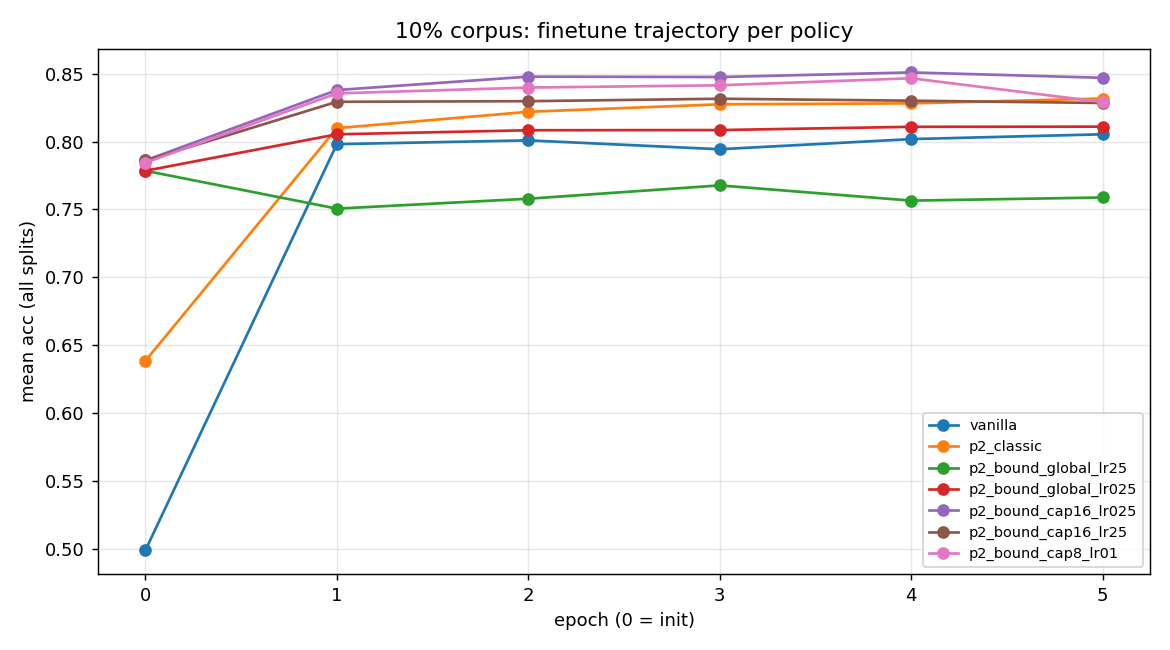
\includegraphics[width=0.75\textwidth]{assets/dbpedia/ft010_curves.png}
    \caption{Fine-tuning trajectory per policy on the 10\% sub-corpus (mean
    accuracy over all 89 splits, standardize lens). The capped bound init
    (\texttt{cap@16}, protected LR) climbs steadily; the un-capped init at the
    protected LR only creeps, and at the full LR \emph{falls below its own
    epoch-0 init} -- turning up the learning rate cannot fix the freeze while the
    $65{,}000$-norm hubs are present.}
    \label{fig:dbpedia_ft010}
\end{figure}

Figure~\ref{fig:dbpedia_ft010} shows three things. (i)~\textbf{The cap works}:
with the hubs capped, the bound embedding climbs from $0.786$ to $0.853$ and
becomes the best single embedding on the sub-corpus, ahead of \texttt{vanilla}
($0.805$) and the classic transfer ($0.832$) on every column. (ii)~\textbf{Raising
the learning rate is not a substitute}: leaving the hubs in place and fine-tuning
at the full rate $0.025$ makes the score \emph{fall below the starting point}
($0.778 \rightarrow 0.759$), because large steps on length-$65{,}000$ vectors
throw them off. (iii)~\textbf{The cap lets the frozen entities learn again}: the
enumerated-individual family (tc04--tc06), stuck at $0.808$ with the un-capped
init, recovers to $0.914$ once the hubs are capped, level with the classic
transfer ($0.915$) and above \texttt{vanilla} ($0.879$).

The same recipe works on the full 1.16B-token corpus: the capped bound embedding
goes from $0.785$ at init to $0.849$ overall ($0.911$ regular, $0.733$ hard),
with the $\{e\}$ family at $0.928$. At full scale it clears \texttt{vanilla}
($0.823$) and edges ahead of the classic transfer ($0.841$ overall), a full
reversal from the un-capped version, which was the worst of the three ($0.808$).
One ceiling on a few thousand hub vectors lifts the worst of the three embeddings
to the best overall, with the margin concentrated on the hard splits.

Table~\ref{tab:dbpedia_cap_p3} breaks this full-corpus result down per test case,
with the classic transfer (\texttt{p3\_classic}) placed alongside for comparison.
The cap lifts the bound embedding everywhere the freeze had blocked it (the
enumerated-individual family tc04--tc06, $\approx 0.79 \rightarrow 0.90$, plus tc03
and tc05), while the constructor families it already won (tc07, tc09) stay ahead.
The classic transfer is the surprise here: it matches the capped bound across the
regular splits (0.914 vs.\ 0.919), takes tc03, tc04 and tc11 outright, and ties the
cap on tc06, so on the easy half of the benchmark the two are level. The cap keeps
its edge only on the hard splits (0.733 vs.\ 0.705), which is enough to stay ahead
overall (0.850 vs.\ 0.841); the un-capped models now hold a single row, tc01-hard,
where their preserved norm tail still helps. P2 and P3 are interchangeable once
capped (0.849 vs.\ 0.850 overall; \texttt{p3\_bound\_cap16} takes the regular mean,
\texttt{p2\_bound\_cap16} the hard mean), confirming once more that protograph depth
is not what decides the outcome here; the cap is.

\begin{table}[t]
\centering
\small
\caption{Norm capping on the \emph{full} 1.16B-token corpus, per test case
(standardize lens, mean over domains; \texttt{\_hard} marks the hard splits).
The two un-capped bound embeddings (\texttt{p2\_bound}, \texttt{p3\_bound}) and
the classic transfer (\texttt{p3\_classic}) are compared against the capped bound
counterparts (\texttt{cap@16}, protected LR). Best per row in bold; the last three
rows are the regular, hard, and overall means (flat over splits).}
\label{tab:dbpedia_cap_p3}
\setlength{\tabcolsep}{4pt}
\begin{tabular}{lcccccc}
\toprule
\textbf{Test case} & $n$ & \textbf{p2\_bound} & \textbf{p3\_bound} & \textbf{p3\_classic}
& \textbf{p2\,cap@16} & \textbf{p3\,cap@16} \\
\midrule
tc01 & 5 & 0.918 & 0.913 & 0.917 & \textbf{0.949} & 0.941 \\
tc01\_hard & 2 & \textbf{0.793} & 0.778 & 0.685 & 0.764 & 0.751 \\
tc02 & 5 & 0.914 & 0.914 & 0.921 & \textbf{0.929} & 0.926 \\
tc02\_hard & 4 & 0.685 & 0.667 & 0.623 & \textbf{0.713} & 0.680 \\
tc03 & 4 & 0.886 & 0.883 & \textbf{0.942} & 0.933 & 0.928 \\
tc04 & 5 & 0.785 & 0.801 & \textbf{0.907} & 0.902 & 0.902 \\
tc04\_hard & 1 & 0.770 & 0.769 & 0.915 & \textbf{0.917} & 0.915 \\
tc05 & 6 & 0.842 & 0.764 & 0.970 & 0.970 & \textbf{0.972} \\
tc06 & 5 & 0.811 & 0.810 & \textbf{0.903} & \textbf{0.903} & \textbf{0.903} \\
tc06\_hard & 1 & 0.777 & 0.728 & 0.873 & 0.871 & \textbf{0.876} \\
tc07 & 2 & 0.971 & 0.965 & 0.980 & \textbf{0.981} & 0.977 \\
tc08 & 3 & 0.864 & 0.868 & 0.911 & \textbf{0.912} & 0.907 \\
tc09 & 5 & 0.893 & 0.893 & 0.891 & \textbf{0.933} & 0.926 \\
tc09\_hard & 5 & 0.826 & 0.808 & 0.792 & \textbf{0.880} & 0.865 \\
tc10 & 6 & 0.842 & 0.849 & 0.853 & 0.872 & \textbf{0.875} \\
tc10\_hard & 6 & 0.671 & 0.651 & 0.645 & \textbf{0.683} & 0.672 \\
tc11 & 6 & 0.813 & 0.907 & \textbf{0.961} & 0.861 & 0.945 \\
tc11\_hard & 6 & 0.697 & 0.667 & \textbf{0.729} & 0.657 & 0.645 \\
tc12 & 6 & 0.833 & 0.814 & 0.859 & 0.853 & \textbf{0.861} \\
tc12\_hard & 6 & 0.670 & 0.643 & 0.665 & \textbf{0.686} & 0.682 \\
\midrule
\textbf{Regular} & & 0.856 & 0.857 & 0.914 & 0.911 & \textbf{0.919} \\
\textbf{Hard} & & 0.717 & 0.694 & 0.705 & \textbf{0.733} & 0.720 \\
\textbf{All (89)} & & 0.808 & 0.801 & 0.841 & 0.849 & \textbf{0.850} \\
\bottomrule
\end{tabular}
\end{table}

Figures~\ref{fig:dbpedia6_final}, \ref{fig:dbpedia6_epochs},
and~\ref{fig:dbpedia6_families} step back to the full six-variant picture with
the capped init dropped back into the headline comparison. To keep all six on one
comparable axis they use the raw lens (the un-standardized features of
Table~\ref{tab:dbpedia_per_tc}) and the full $1.16$B-token corpus rather than the
standardize lens and controlled sub-corpus above; the per-epoch panels average
flatly over the $89$ splits. On this footing the capped bound init reaches $0.852$
overall, slightly ahead of \texttt{p2\_classic} ($0.844$) and clearly above
\texttt{vanilla} ($0.831$), and leads every variant on the hard splits ($0.742$). It restores the
enumerated-individual families tc04--tc06 ($0.79 \rightarrow 0.93$ on the hard
splits) and the typed-cardinality cases tc11/tc12 where the un-capped
\texttt{p2\_bound} drops below \texttt{vanilla}, while preserving the bound's edge
on tc07 and tc09 (Figure~\ref{fig:dbpedia6_final}); per epoch it tracks the
classic transfers on the regular splits and sits above all variants on the hard
splits, whereas the un-capped bound stays frozen near its epoch-0 value
(Figures~\ref{fig:dbpedia6_epochs} and~\ref{fig:dbpedia6_families}).

\begin{figure}[t]
    \centering
    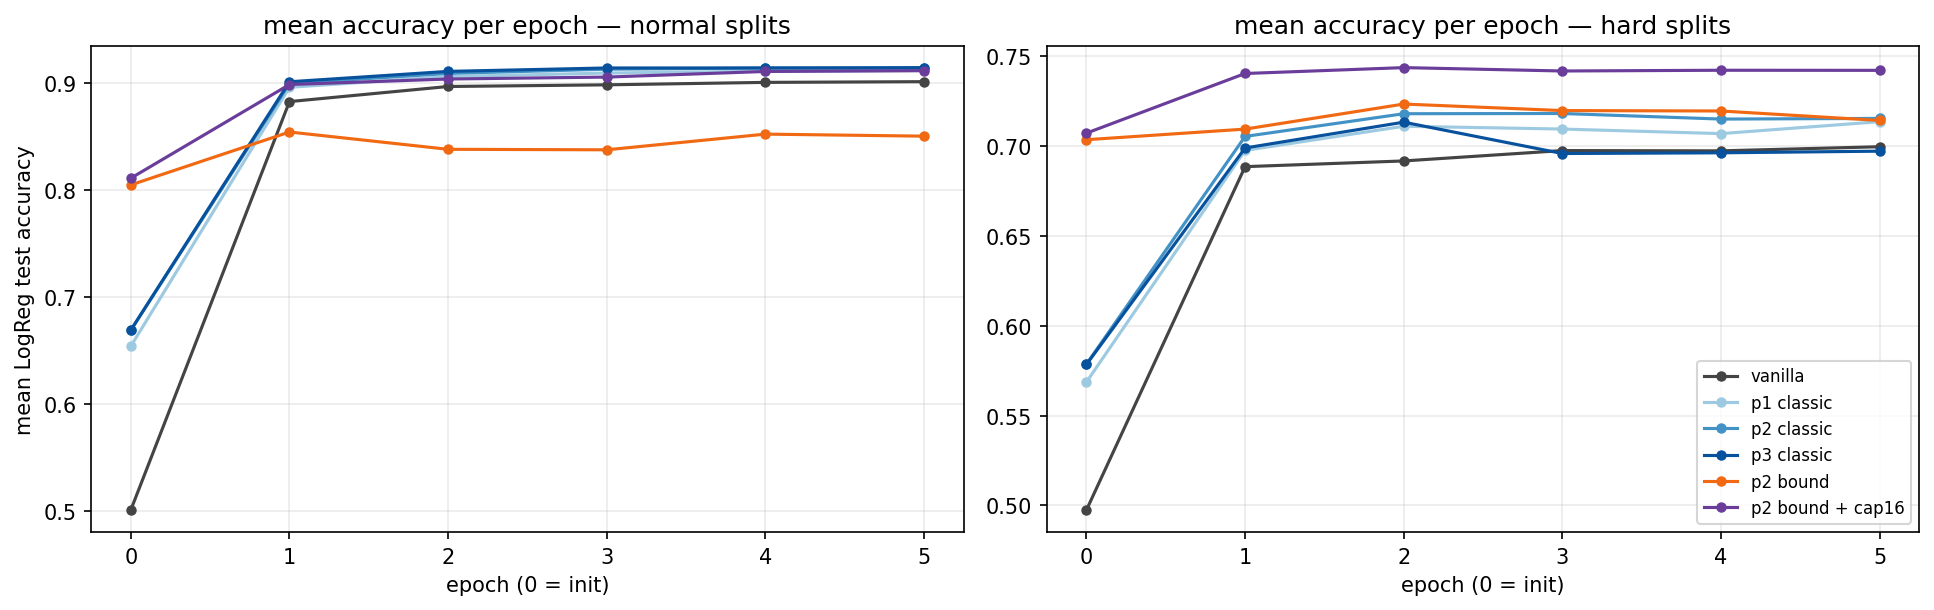
\includegraphics[width=\textwidth]{assets/dbpedia/acc_per_epoch_normal_hard.png}
    \caption{Mean test accuracy per fine-tuning epoch (flat mean over the $89$
    splits, raw lens, full corpus), regular (left) and hard (right) splits;
    epoch~0 is the initialization. The capped bound init tracks the classic
    transfers at the top on the regular splits and leads every variant on the
    hard splits, whereas the un-capped \texttt{p2\_bound} stays frozen near its
    epoch-0 value on the regular splits.}
    \label{fig:dbpedia6_epochs}
\end{figure}

\begin{figure}[t]
    \centering
    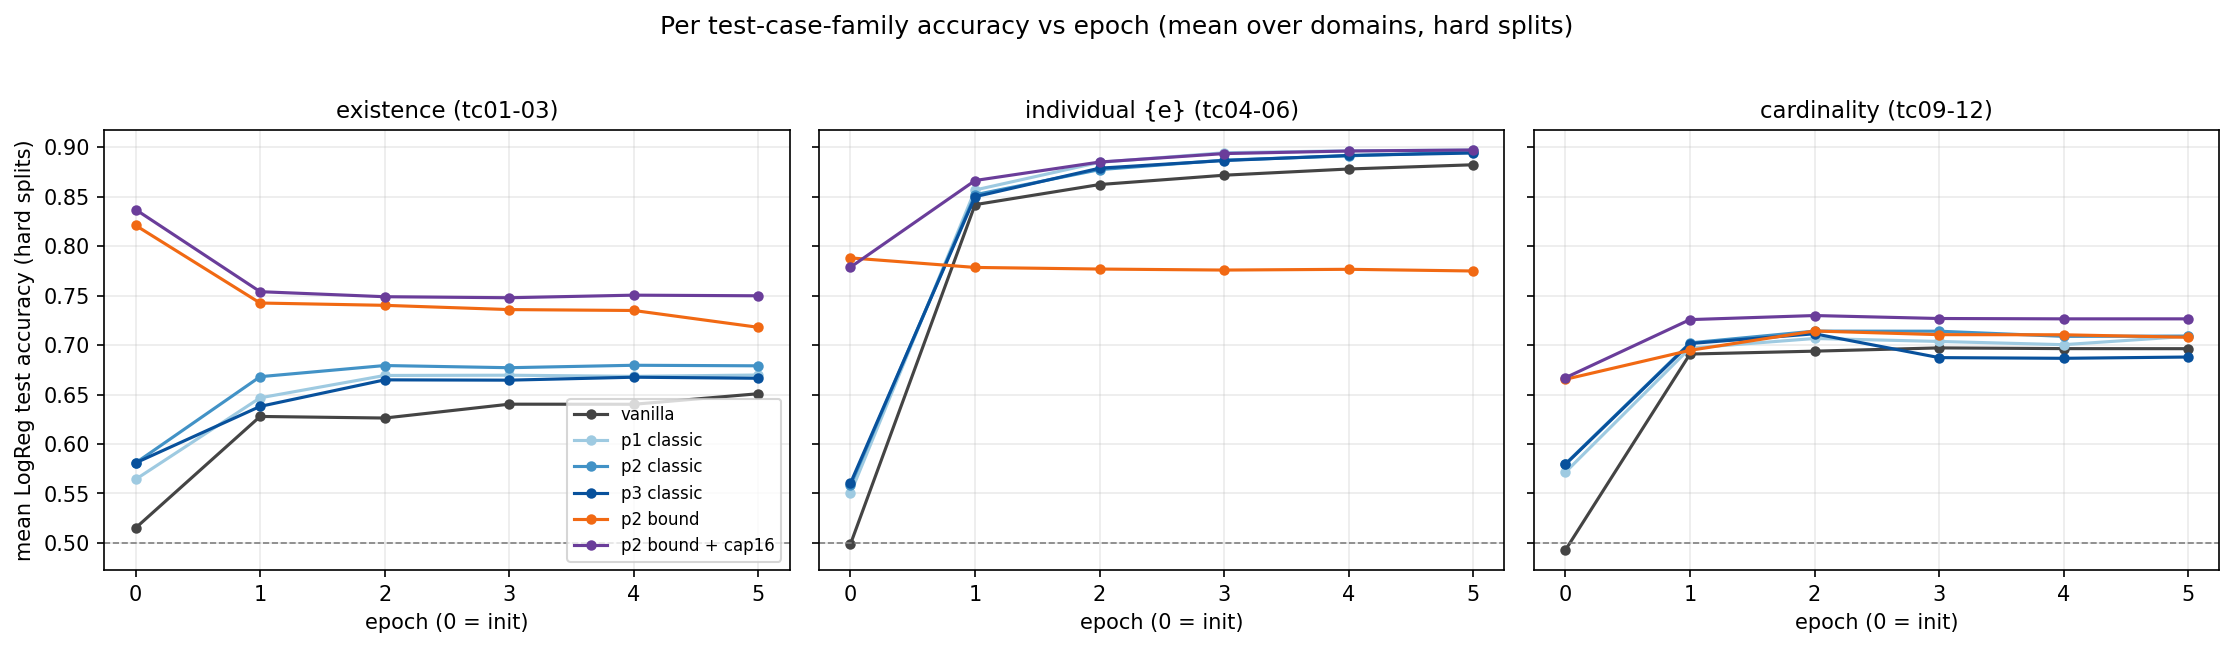
\includegraphics[width=\textwidth]{assets/dbpedia/acc_per_epoch_domains.png}
    \caption{Per test-case-family accuracy per fine-tuning epoch on the hard
    splits (mean over domains, raw lens, full corpus). The qualified-existential
    family (tc07--tc08) has no hard splits and is omitted. The cap recovers the
    enumerated-individual family (tc04--tc06) that the un-capped bound freezes,
    and leads on the existence and cardinality families.}
    \label{fig:dbpedia6_families}
\end{figure}

\subsection{Compressing Counts During Construction: \texttt{log1p} and \texttt{sqrt}}
\label{sec:dbpedia_compress}

The cap works, but it is a post-hoc patch with a threshold to choose: build the
init, then clip whatever exceeds $\tau=16$. A cleaner option is to never let the
tail form. The hub norms blow up because the construction \emph{accumulates} one
unit vector per (edge, neighbour-class) pair, so an entity with tens of thousands
of edges piles up a norm in the tens of thousands. We damp this at the source by
rescaling each row $v$ through a monotone squashing function $f$ while the init is
built,
\begin{equation*}
  v \;\leftarrow\; v \cdot \frac{f(\lVert v \rVert)}{\lVert v \rVert},
  \qquad f(n) = \log(1+n) \ \text{(\texttt{log1p})} \quad\text{or}\quad
  f(n) = \sqrt{n}\ \text{(\texttt{sqrt})},
\end{equation*}
applied before the usual global rescale to mean norm $8$, with the direction left
unchanged as for the cap. Both functions grow without bound, so unlike the cap
they keep \emph{every} entity distinguishable, yet slowly enough that the heavy
tail collapses: $\log(1+n)$ turns a raw norm of $65{,}000$ into $\approx 11$, with
no threshold to choose.

Table~\ref{tab:dbpedia_compress} traces this on the 10\% sub-corpus, ordered by
how much of the init norm tail survives. The trend is consistent: as the largest
init norm falls from the un-capped $65{,}339$ through $\sqrt{}$'s $979$ to
\texttt{log1p}'s $47$ and the cap's $16$, the final accuracy rises
($0.811 \rightarrow 0.841 \rightarrow 0.853$) and then plateaus, with
\texttt{log1p} and \texttt{cap@16} tied at $0.853$ despite their different norms.
This is the clearest evidence in this section that the \emph{norm tail, not the
binding construction}, drove the freeze.

\begin{table}[t]
\centering
\small
\caption{Count compression vs.\ the post-hoc cap (10\% sub-corpus, standardize
lens, flat mean over 89 splits). \emph{Max $\lVert\cdot\rVert$} is the largest
entity-row norm in the init; \emph{Init} is epoch~0 and \emph{Final} epoch~5;
\emph{card-H} is the cardinality-hard family (tc09--12) and \emph{$\{e\}$} the
regular enumerated-individual family (tc04--06). The rows are ordered by init
norm tail. Best per column in bold.}
\label{tab:dbpedia_compress}
\setlength{\tabcolsep}{5pt}
\begin{tabular}{lccccccc}
\toprule
\textbf{Init} & \textbf{max $\lVert\cdot\rVert$} & \textbf{Init} & \textbf{Final}
& \textbf{Regular} & \textbf{Hard} & \textbf{card-H} & \textbf{$\{e\}$} \\
\midrule
un-capped (global) & 65339 & 0.778 & 0.811 & 0.864 & 0.711 & 0.698 & 0.808 \\
\texttt{sqrt}      & 979   & 0.787 & 0.841 & 0.898 & 0.732 & 0.719 & 0.884 \\
\texttt{cap@16}    & 16    & 0.786 & \textbf{0.853} & 0.909 & \textbf{0.748} & 0.726 & \textbf{0.914} \\
\texttt{log1p}     & 47    & 0.784 & \textbf{0.853} & \textbf{0.910} & 0.746 & \textbf{0.736} & 0.910 \\
\bottomrule
\end{tabular}
\end{table}

\textbf{\texttt{log1p} is the keeper.} It reproduces the cap's result (0.853
overall, $0.856$ on the full corpus, matching the capped $0.849$--$0.850$)
\emph{without} the post-hoc clip or its threshold, the init norms simply topping
out at $\approx 47$ instead of $\approx 65{,}000$. It even edges the cap on the
cardinality-hard family ($0.736$ vs.\ $0.726$): a smooth squash preserves
low-count resolution slightly better than a hard clip, which flattens everything
above $16$ to the same length. It is the cleaner default construction.

\textbf{\texttt{sqrt} is the cautionary control.} It compresses too gently (the
init still reaches a norm of $979$), so a residual tail survives, the hub rows
re-freeze, and the $\{e\}$ sink partly returns (tc04--06 back to $0.884$ against
the cap's $0.914$), holding the model to $0.841$: still above \texttt{vanilla}
and the un-capped init, but the weakest of the tail-taming variants. A
\emph{milder} version of the same idea recovering less of the accuracy is
consistent with the reading that the residual tail, not the binding, sets the
ceiling.

\subsection{Specificity-Weighted Initialization}
\label{sec:dbpedia_specificity}

Capping and compression change the \emph{magnitude} of the init. This subsection
asks whether reshaping its \emph{content} helps. The own-class term averages the
codes of an entity's types with equal weight. After \texttt{owl:Thing} is
removed, that mean still mixes a specific leaf type (\textit{SoccerPlayer}) with
generic ancestors (\textit{Athlete}, \textit{Person}, \textit{Agent}) shared by
millions of entities, which might dilute the discriminative signal. We therefore
weight each class code by its specificity, using inverse document frequency:
\begin{equation*}
  w_c = \log\frac{N}{\mathrm{df}_c},
\end{equation*}
where $\mathrm{df}_c$ is the number of entities whose type set contains class $c$
and $N$ is the number of typed entities. A near-universal class (\textit{Agent})
gets a weight near zero; a rare leaf type gets a large one. Only the own-class
term changes; the cap, the learning rate, and the other channels stay fixed.

In aggregate the reweighting changes nothing (Table~\ref{tab:dbpedia_idf}): the
IDF init finishes at $0.851$ against the uniform cap@16 control's $0.853$, inside
the $\approx\!0.003$ run-to-run noise. Individual cells move but cancel.
Specificity helps where the discriminative concept is a leaf type (tc11 $0.919
\rightarrow 0.933$) and hurts where it is an inherited superclass (tc02-hard
$0.780 \rightarrow 0.715$, pulling the existence-hard family from $0.788$ to
$0.747$). On a benchmark that mixes both, it nets to a wash.

\begin{table}[t]
\centering
\small
\caption{Specificity (IDF) weighting of the own-class term, against the uniform
cap@16 control (10\% sub-corpus, standardize lens, flat mean over 89 splits).
\emph{exist-H}, \emph{indiv-H}, and \emph{card-H} are the hard existence
(tc01--03), enumerated-individual (tc04--06), and cardinality (tc09--12)
families. The overall mean is unchanged (within run-to-run noise), but the
reweighting trades small gains on leaf-type splits for a larger loss on
existence-hard (exist-H $-0.041$); it cancels only in the aggregate.}
\label{tab:dbpedia_idf}
\setlength{\tabcolsep}{5pt}
\begin{tabular}{lccccccc}
\toprule
\textbf{Init} & \textbf{Init$_0$} & \textbf{Final} & \textbf{Regular} & \textbf{Hard}
& \textbf{exist-H} & \textbf{indiv-H} & \textbf{card-H} \\
\midrule
cap@16 (uniform) & 0.786 & 0.853 & 0.909 & 0.748 & 0.788 & 0.883 & 0.726 \\
cap@16 + IDF     & 0.787 & 0.851 & 0.909 & 0.742 & 0.747 & 0.880 & 0.729 \\
\midrule
$\Delta$         & $+0.001$ & $-0.002$ & $0.000$ & $-0.006$ & $-0.041$ & $-0.003$ & $+0.003$ \\
\bottomrule
\end{tabular}
\end{table}

\subsection{Hierarchy Weighting: \texttt{bound\_decay} and \texttt{bound\_specific}}
\label{sec:dbpedia_hierarchy}

The previous knob reweighted only the own-class term. This one reweights the
whole type hierarchy. By default the init gives every type of an entity equal
weight: its most specific class \emph{and} all of its superclasses
(\texttt{uniform}). A deeply nested type therefore brings in a lot of generic
superclass mass. We test two alternatives:
\begin{itemize}
  \item \texttt{decay}: keep all superclasses but fade them with distance from
  the leaf, weighting a class by $0.5^{\,\mathrm{hops}}$ (leaf $1$, parent $0.5$,
  grandparent $0.25$, \dots);
  \item \texttt{most\_specific}: drop the superclasses and keep only the single
  most specific class.
\end{itemize}

\paragraph{The right amount of hierarchy depends on the task (synthetic).}
On the synthetic suite the three weightings split cleanly by what each task needs
(Table~\ref{tab:hierarchy_synth}). In tc07 ($\exists r.C$ with leaf-typed
objects), the class that matters, $C$, is a superclass of the objects' own types,
so the answer sits in the superclasses: keeping them all (\texttt{uniform}) is
best ($0.993$), and dropping them hurts (\texttt{most\_specific} $0.835$). In the
counting task tc09 ($\geq 2r$) what matters is an edge count, and in the
own-class-membership task tc14 the label \emph{is} the entity's own most-specific
class; in both the generic superclasses only add noise, so dropping them helps:
\texttt{decay} wins tc09 ($0.895$) and \texttt{most\_specific} wins tc14
($0.981$). \texttt{decay} is the
safe middle: best or near-best on these tasks with only a small loss on
tc07.

\begin{table}[t]
\centering
\small
\caption{Hierarchy weighting on the synthetic suite (epoch-5 accuracy, P2). The
best weighting follows the task: keep the full hierarchy when the answer is an
inherited superclass (tc07), drop it when the answer is an edge count (tc09) or
the entity's own most-specific class (tc14).
Best per row in bold.}
\label{tab:hierarchy_synth}
\setlength{\tabcolsep}{6pt}
\begin{tabular}{lcccc}
\toprule
\textbf{Test case} & \textbf{vanilla} & \textbf{uniform} & \textbf{decay} & \textbf{most-specific} \\
\midrule
tc07 ($\exists r.C$, leaf-typed) & 0.583 & \textbf{0.993} & 0.955 & 0.835 \\
tc09 ($\geq 2\,r$, counting)     & 0.635 & 0.848 & \textbf{0.895} & 0.877 \\
tc14 (own-class membership)      & 0.663 & 0.905 & 0.958 & \textbf{0.981} \\
\bottomrule
\end{tabular}
\end{table}

\paragraph{On full DBpedia the cap matters far more than the weighting.}
We run all four combinations of weighting (\texttt{decay},
\texttt{most\_specific}) and norm policy (global rescale, cap@16) on the full
corpus, next to the uniform base and the vanilla reference
(Table~\ref{tab:dbpedia_hierarchy}). Two things stand out. First, the weighting
alone barely changes the init: without the cap all three weightings sit at
$\approx\!0.81$ (decay $0.811$, uniform $0.808$, most-specific $0.806$) and still
fall \emph{below} vanilla ($0.823$). This is the frozen-hub problem again, and a
different class weighting cannot fix it while the global rescale leaves the hubs
in place. The cap is what lifts every weighting by about $4$ points (e.g.\
uniform $0.808 \rightarrow 0.850$, decay $0.811 \rightarrow 0.860$), carrying it
clear of vanilla ($0.823$).
Second, once the init is capped the weighting does help a little: \texttt{decay}
+ cap@16 is the best bound embedding on full DBpedia at \textbf{0.860}, $+0.037$
over vanilla and $+0.010$ over the uniform cap@16 base. The gain is small overall
but shows up where a cleaner hierarchy should help: the hard splits ($0.756$ vs.\
$0.737$) and the cardinality-hard family ($0.738$ vs.\ $0.720$), matching the
synthetic counting result. \texttt{decay} edges out \texttt{most\_specific}
($0.860$ vs.\ $0.849$), but most-specific still has a use: it keeps the best
enumerated-individual family (indiv-H $0.902$), since keeping only the leaf type
sharpens the individual signal at the cost of the superclass mass the hard
existence splits rely on.

\begin{table}[t]
\centering
\small
\caption{Hierarchy weighting $\times$ norm policy on the \emph{full} corpus
(standardize lens, flat mean over 89 splits). \emph{card-H} and \emph{indiv-H}
are the cardinality-hard (tc09--12) and enumerated-individual-hard (tc04--06)
families. The cap changes accuracy by about $4$ points, the weighting by about
$1$. Best per column in bold; reference rows use the same harness.}
\label{tab:dbpedia_hierarchy}
\setlength{\tabcolsep}{5pt}
\begin{tabular}{llcccccc}
\toprule
\textbf{Weighting} & \textbf{norm} & \textbf{Init} & \textbf{Final}
& \textbf{Regular} & \textbf{Hard} & \textbf{card-H} & \textbf{indiv-H} \\
\midrule
\texttt{vanilla} (ref) & --     & --    & 0.823 & 0.894 & 0.691 & 0.687 & 0.869 \\
\midrule
uniform        & global & --    & 0.808 & 0.856 & 0.717 & 0.711 & 0.773 \\
decay          & global & 0.782 & 0.811 & 0.862 & 0.714 & 0.708 & 0.772 \\
most-specific  & global & 0.778 & 0.806 & 0.853 & 0.719 & 0.712 & 0.783 \\
\midrule
uniform        & cap@16 & 0.785 & 0.850 & 0.911 & 0.737 & 0.720 & 0.892 \\
decay          & cap@16 & \textbf{0.790} & \textbf{0.860} & \textbf{0.915} & \textbf{0.756} & \textbf{0.738} & 0.896 \\
most-specific  & cap@16 & 0.784 & 0.849 & 0.912 & 0.730 & 0.723 & \textbf{0.902} \\
\bottomrule
\end{tabular}
\end{table}

Of all the construction-side knobs in this and the previous two subsections, only
one adds to the cap, and only by a little: decay-weighting the hierarchy. It
gives the best bound embedding on full DBpedia, \texttt{p2\_bound\_decay\_cap16}
at $0.860$ ($+0.037$ over vanilla), with its edge on the hard and cardinality
splits the construction targets. The cap is still the decisive ingredient; the
weighting is a small refinement on top of it, and \texttt{decay} ($0.5$) is the
safe default, in line with the synthetic result.

\subsection{Ablations: Cap Size and Learning Rate}
\label{sec:dbpedia_ablations}

The capped-init recipe has two hyperparameters that earlier subsections took as
given: the cap threshold $\tau$ and the protected fine-tuning learning rate. Here
we fix both. Both ablations run on the 10\% sub-corpus.

\paragraph{Cap size.} We sweep $\tau \in \{2,4,8,16,32,64,\infty\}$, where
$\infty$ means no cap. We read the \emph{epoch-0} init quality, that is, how much
the clip distorts the init on its own, before any fine-tuning
(Table~\ref{tab:dbpedia_capsize}, Figure~\ref{fig:dbpedia_capsweep}). The curve is
almost flat. Every cap from $4$ to $64$ lands within $0.002$ of the others.
Capping at $\tau=16$ even \emph{improves} the un-capped init a little, from
$0.777$ to $0.785$ overall. The reason is simple: the heavy hubs the clip touches
are rarely the entities a DLCC split tests. The cardinality-hard family is the
most exposed, since its signal lives in the vector magnitude. It still holds up
down to $\tau\approx 8$ ($0.671$--$0.674$) and only drops at the tightest cap
$\tau=2$ ($0.655$), where the clip starts biting into ordinary entities. $\tau=16$
is the (marginal) best on every column, so that is the value we use. The wide
plateau matters more than the peak: the cap is a safe unfreeze, not a setting that
needs careful tuning. P3 behaves the same way (Figure~\ref{fig:dbpedia_capsweep}).

\begin{table}[t]
\centering
\small
\caption{Cap-size sweep on the P2 concept-bound init (epoch-0 quality, 10\%
testbed, standardize lens). $\tau=\infty$ is the un-capped init; \emph{card-H} is
the cardinality-hard family (tc09--12), whose signal lives in the vector
magnitude and is therefore the most exposed to clipping. Best per column in bold.}
\label{tab:dbpedia_capsize}
\setlength{\tabcolsep}{6pt}
\begin{tabular}{lcccc}
\toprule
\textbf{cap $\tau$} & \textbf{all} & \textbf{regular} & \textbf{hard} & \textbf{card-H} \\
\midrule
$\infty$ (no cap) & 0.777 & 0.822 & 0.694 & 0.662 \\
2  & 0.776 & 0.824 & 0.687 & 0.655 \\
4  & 0.783 & 0.828 & 0.699 & 0.669 \\
8  & 0.783 & 0.828 & 0.700 & 0.671 \\
16 & \textbf{0.785} & \textbf{0.829} & \textbf{0.703} & \textbf{0.674} \\
32 & 0.783 & 0.826 & 0.702 & 0.672 \\
64 & 0.783 & 0.826 & 0.702 & 0.671 \\
\bottomrule
\end{tabular}
\end{table}

\begin{figure}[t]
    \centering
    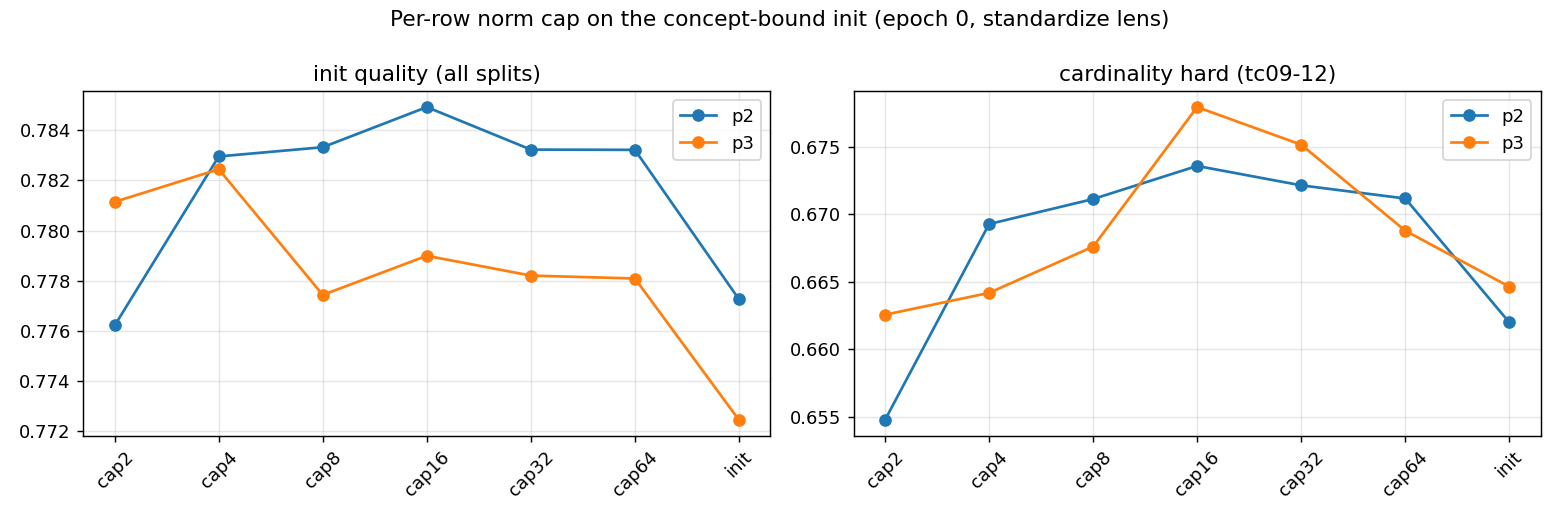
\includegraphics[width=0.85\textwidth]{assets/dbpedia/norm_cap_sweep.png}
    \caption{Per-row norm cap on the concept-bound init (epoch 0, standardize
    lens) for P2 and P3. Left: overall init quality; right: the cardinality-hard
    family. Both are flat across a broad range of caps and peak near $\tau=16$;
    only very tight caps ($\tau=2$) erode the cardinality signal.}
    \label{fig:dbpedia_capsweep}
\end{figure}

\paragraph{Learning rate.} The cap removed the $\sim\!65{,}000$-norm hubs that
forced the tiny protected rate in the first place. With the tail gone, a fair
question is whether larger fine-tuning steps now help. They do not
(Table~\ref{tab:dbpedia_lr}, Figure~\ref{fig:dbpedia_exp6curves}). A higher rate
cuts the training loss sharply, from $24.1$M at the protected $0.0025$ to $19.8$M
at $0.01$. But it also \emph{lowers} accuracy on the hard splits, from $0.748$ to
$0.737$. This is the usual sign of over-fitting a corpus the model has already
saturated. A warmup schedule matches the control on the overall mean ($0.853$) but
not on the hard splits ($0.745$ vs.\ $0.748$), and the constant higher rates trail
by about $0.4$ point overall. The protected $0.0025$ was already the right choice.
Once the norm tail is handled, the optimizer has nothing more to give.

\begin{table}[t]
\centering
\small
\caption{Fine-tuning learning-rate schedules on the capped (cap@16) init (10\%
sub-corpus, standardize lens). \emph{loss} is the final-epoch training loss
(millions). Lower loss at higher rates coincides with \emph{lower} hard-split
accuracy, the sign of over-fitting the saturated corpus, so it is not bolded. Best
accuracy per column in bold.}
\label{tab:dbpedia_lr}
\setlength{\tabcolsep}{6pt}
\begin{tabular}{lccccc}
\toprule
\textbf{LR schedule} & \textbf{all} & \textbf{regular} & \textbf{hard} & \textbf{card-H} & \textbf{loss} \\
\midrule
$0.0025 \!\rightarrow\! 10^{-4}$ (protected) & \textbf{0.853} & 0.909 & \textbf{0.748} & \textbf{0.726} & 24.1 \\
warmup $5\mathrm{e}{-4}\!\rightarrow\!5\mathrm{e}{-3}\!\rightarrow\!10^{-4}$ & \textbf{0.853} & \textbf{0.911} & 0.745 & 0.724 & 21.5 \\
$0.005 \!\rightarrow\! 5\mathrm{e}{-4}$ & 0.849 & 0.909 & 0.738 & 0.719 & 21.2 \\
$0.01 \!\rightarrow\! 5\mathrm{e}{-4}$  & 0.849 & 0.908 & 0.737 & 0.724 & 19.8 \\
\bottomrule
\end{tabular}
\end{table}

\begin{figure}[t]
    \centering
    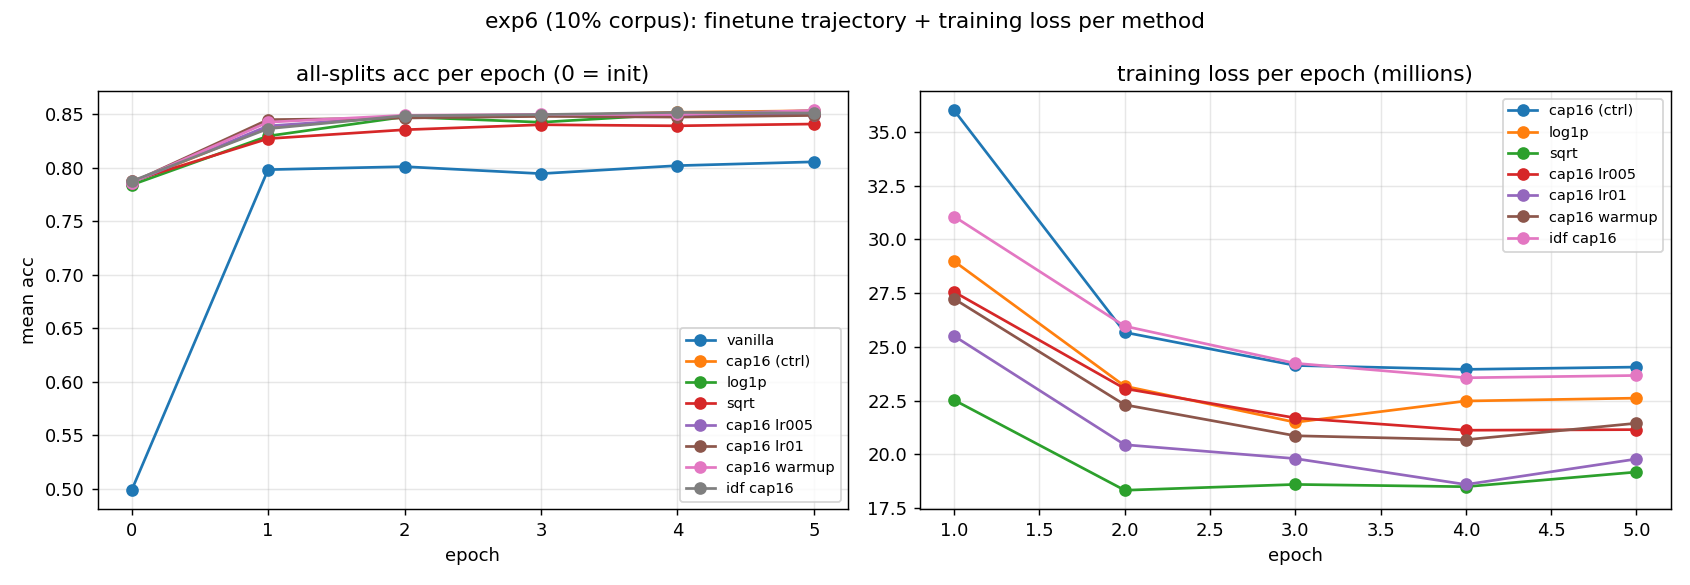
\includegraphics[width=\textwidth]{assets/dbpedia/exp6_curves.png}
    \caption{Fine-tuning trajectory (left) and training loss (right) per method on
    the 10\% sub-corpus. Higher learning rates drive the loss lower but do not
    lift the test accuracy, and on the hard splits they lower it slightly. This is
    the over-fitting signature. The compression variants (\texttt{log1p},
    \texttt{sqrt}) and the IDF prior track the cap@16 control.}
    \label{fig:dbpedia_exp6curves}
\end{figure}

Both ablations point the same way as the rest of the section. The cap is robust
and forgiving: a broad plateau of safe thresholds, with $\tau=16$ the marginal
best. The protected learning rate it was paired with was already optimal. The one
decisive ingredient on DLCC-DBpedia is taming the init's norm tail. Once that is
done, neither the cap threshold nor the optimizer adds anything, and only the
decay hierarchy weighting of the previous subsection gives a small, consistent
gain on top.

\subsection{Embedding-Space Class Separation}
\label{sec:dbpedia_class_separation}

The accuracies so far say which constructor families each init solves, but not
what its embedding space looks like once fine-tuned. We turn to that geometry
here, and then (Section~\ref{sec:dbpedia_geval}) to whether any of it survives on
standard downstream tasks.

Figure~\ref{fig:dbpedia_class_separation} projects the fine-tuned entity
vectors to two dimensions and colours them by entity type (Person, Movies,
Books, Albums, Cities, Countries). The two grids are stacked: the upper grid
uses PCA and the lower grid uses t-SNE. Each grid shows the same panels, with
the \texttt{vanilla} baseline alongside the classic
(\texttt{p1}/\texttt{p2}/\texttt{p3}) and bound variants.

The PCA grid shows the contrast most clearly. For \texttt{vanilla} the types are
mixed together: the classes form one diffuse cloud, so the separation is noisy
and weak. The classic variants break the entities into compact, well-separated
clusters by class. The bound variants separate the classes far less, and this is
worst for the uncapped bound inits. Their PCA collapses: a few vectors dominate
the projection and squeeze the rest into a small region, so almost no class
structure is visible. Adding the cap (\texttt{cap16}) recovers part of the
structure, with some classes pulling out along the dominant axes while the rest
stay jumbled near the origin. The t-SNE grid rescales local distances, so it
recovers clusters even for the uncapped bound. However, the classes still mix
more than under the classic transfer, and the Countries entities in particular
stretch into a long arc that threads through the other types.

This is no surprise. The classic transfer puts every entity of a class in
essentially the same spot (its class code), so the classes are very compact and
easy to separate. The bound init does not do this on purpose: it makes a
compromise between keeping class information and keeping information about the
entity's relations, so entities of the same class are pulled apart by how they
are connected.

A likely reason this compromise costs more separation on DBpedia than on the
synthetic benchmark is the relations themselves. In the synthetic data the
relations are strict: each relation has a single domain and a single range, so it
is very distinct and binding it into an entity adds a clean class signal. DBpedia
relations are much looser. Many of them are used across very different domains
and ranges. For example, a relation like \texttt{city} can link an organization
to a city or a person to a city, so the same relation is shared by entities of
unrelated types. Because the bound init folds the relation signal into the
entity vector, two entities that share such a relation but belong to different
classes get pulled together. The relation blurs them, and in aggregate it mixes
the classes that the classic transfer keeps apart.

\begin{figure}[p]
  \centering
  \begin{subfigure}{\textwidth}
      \centering
      \makebox[\linewidth][c]{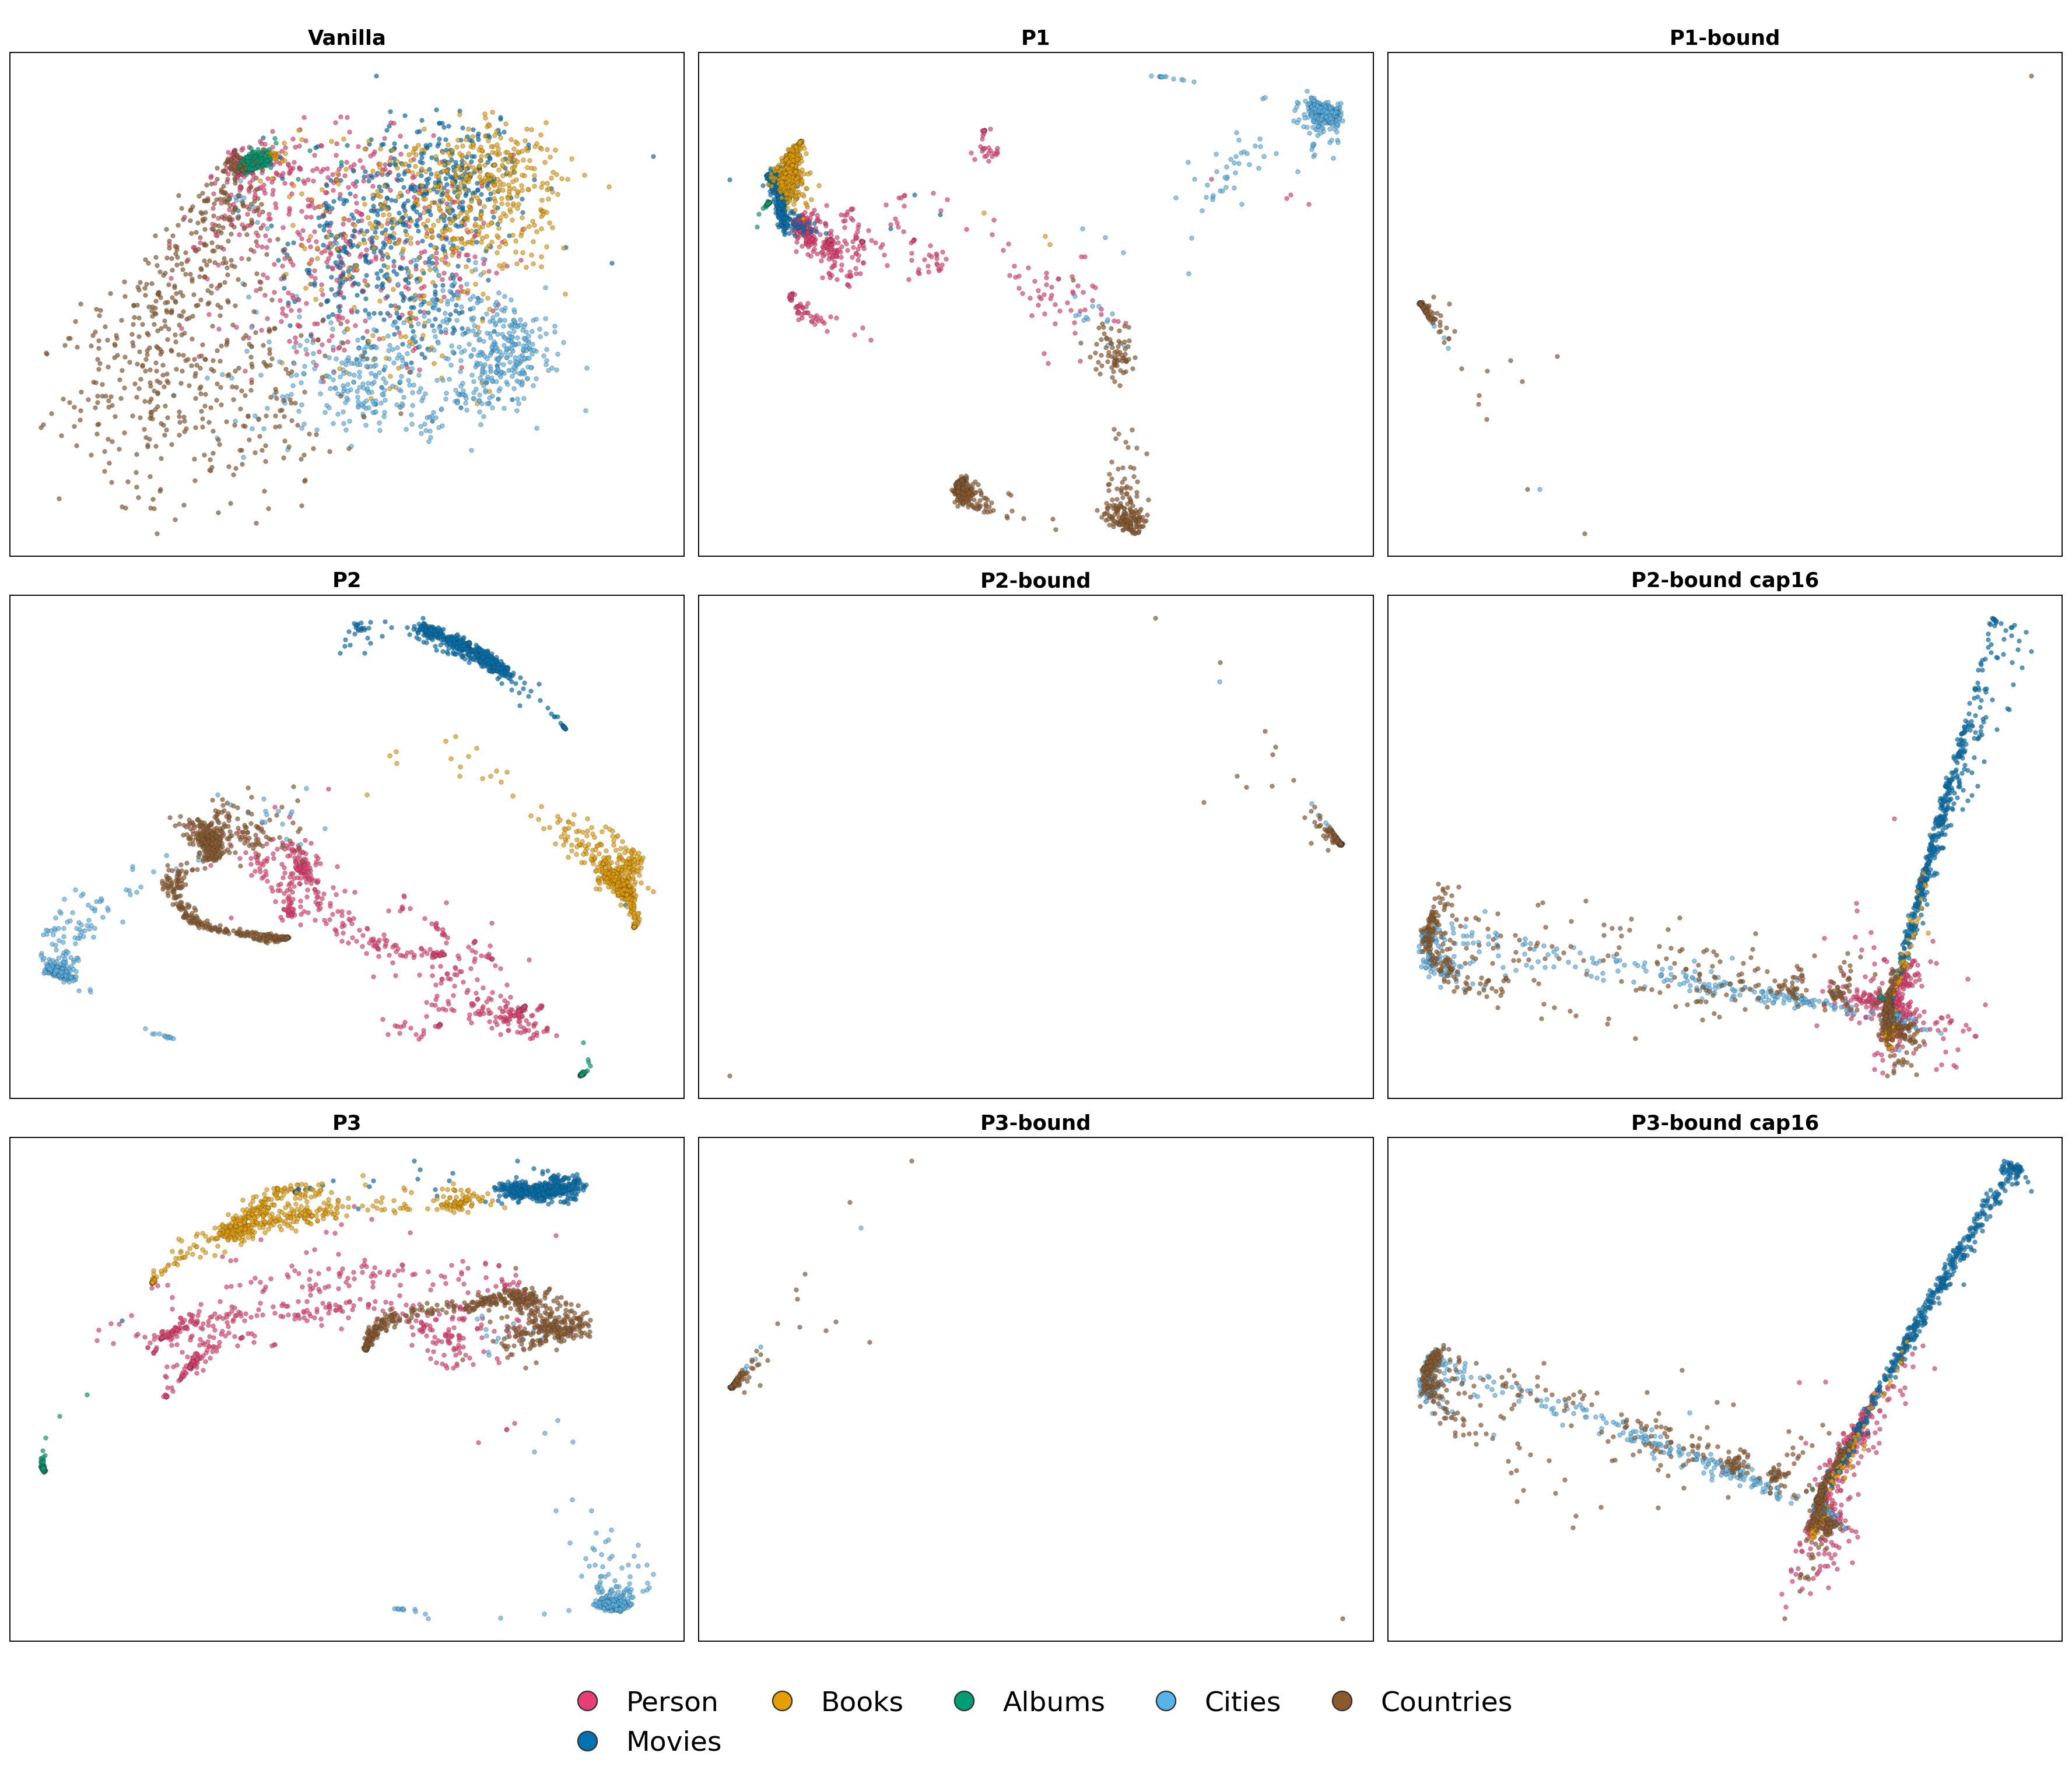
\includegraphics[width=\dimexpr\paperwidth-3cm\relax]{assets/dbpedia/pca_tsne_embedding_plot/dbpedia_schema_fine_pca.png}}
      \caption{PCA}
      \label{fig:dbpedia_class_separation_pca}
  \end{subfigure}
  \caption{Two-dimensional projections of the fine-tuned DBpedia entity
  embeddings, coloured by entity type, for the \texttt{vanilla} baseline and
  the classic and bound variants.}
  \label{fig:dbpedia_class_separation}
\end{figure}

\begin{figure}[p]
  \ContinuedFloat
  \centering
  \begin{subfigure}{\textwidth}
      \centering
      \makebox[\linewidth][c]{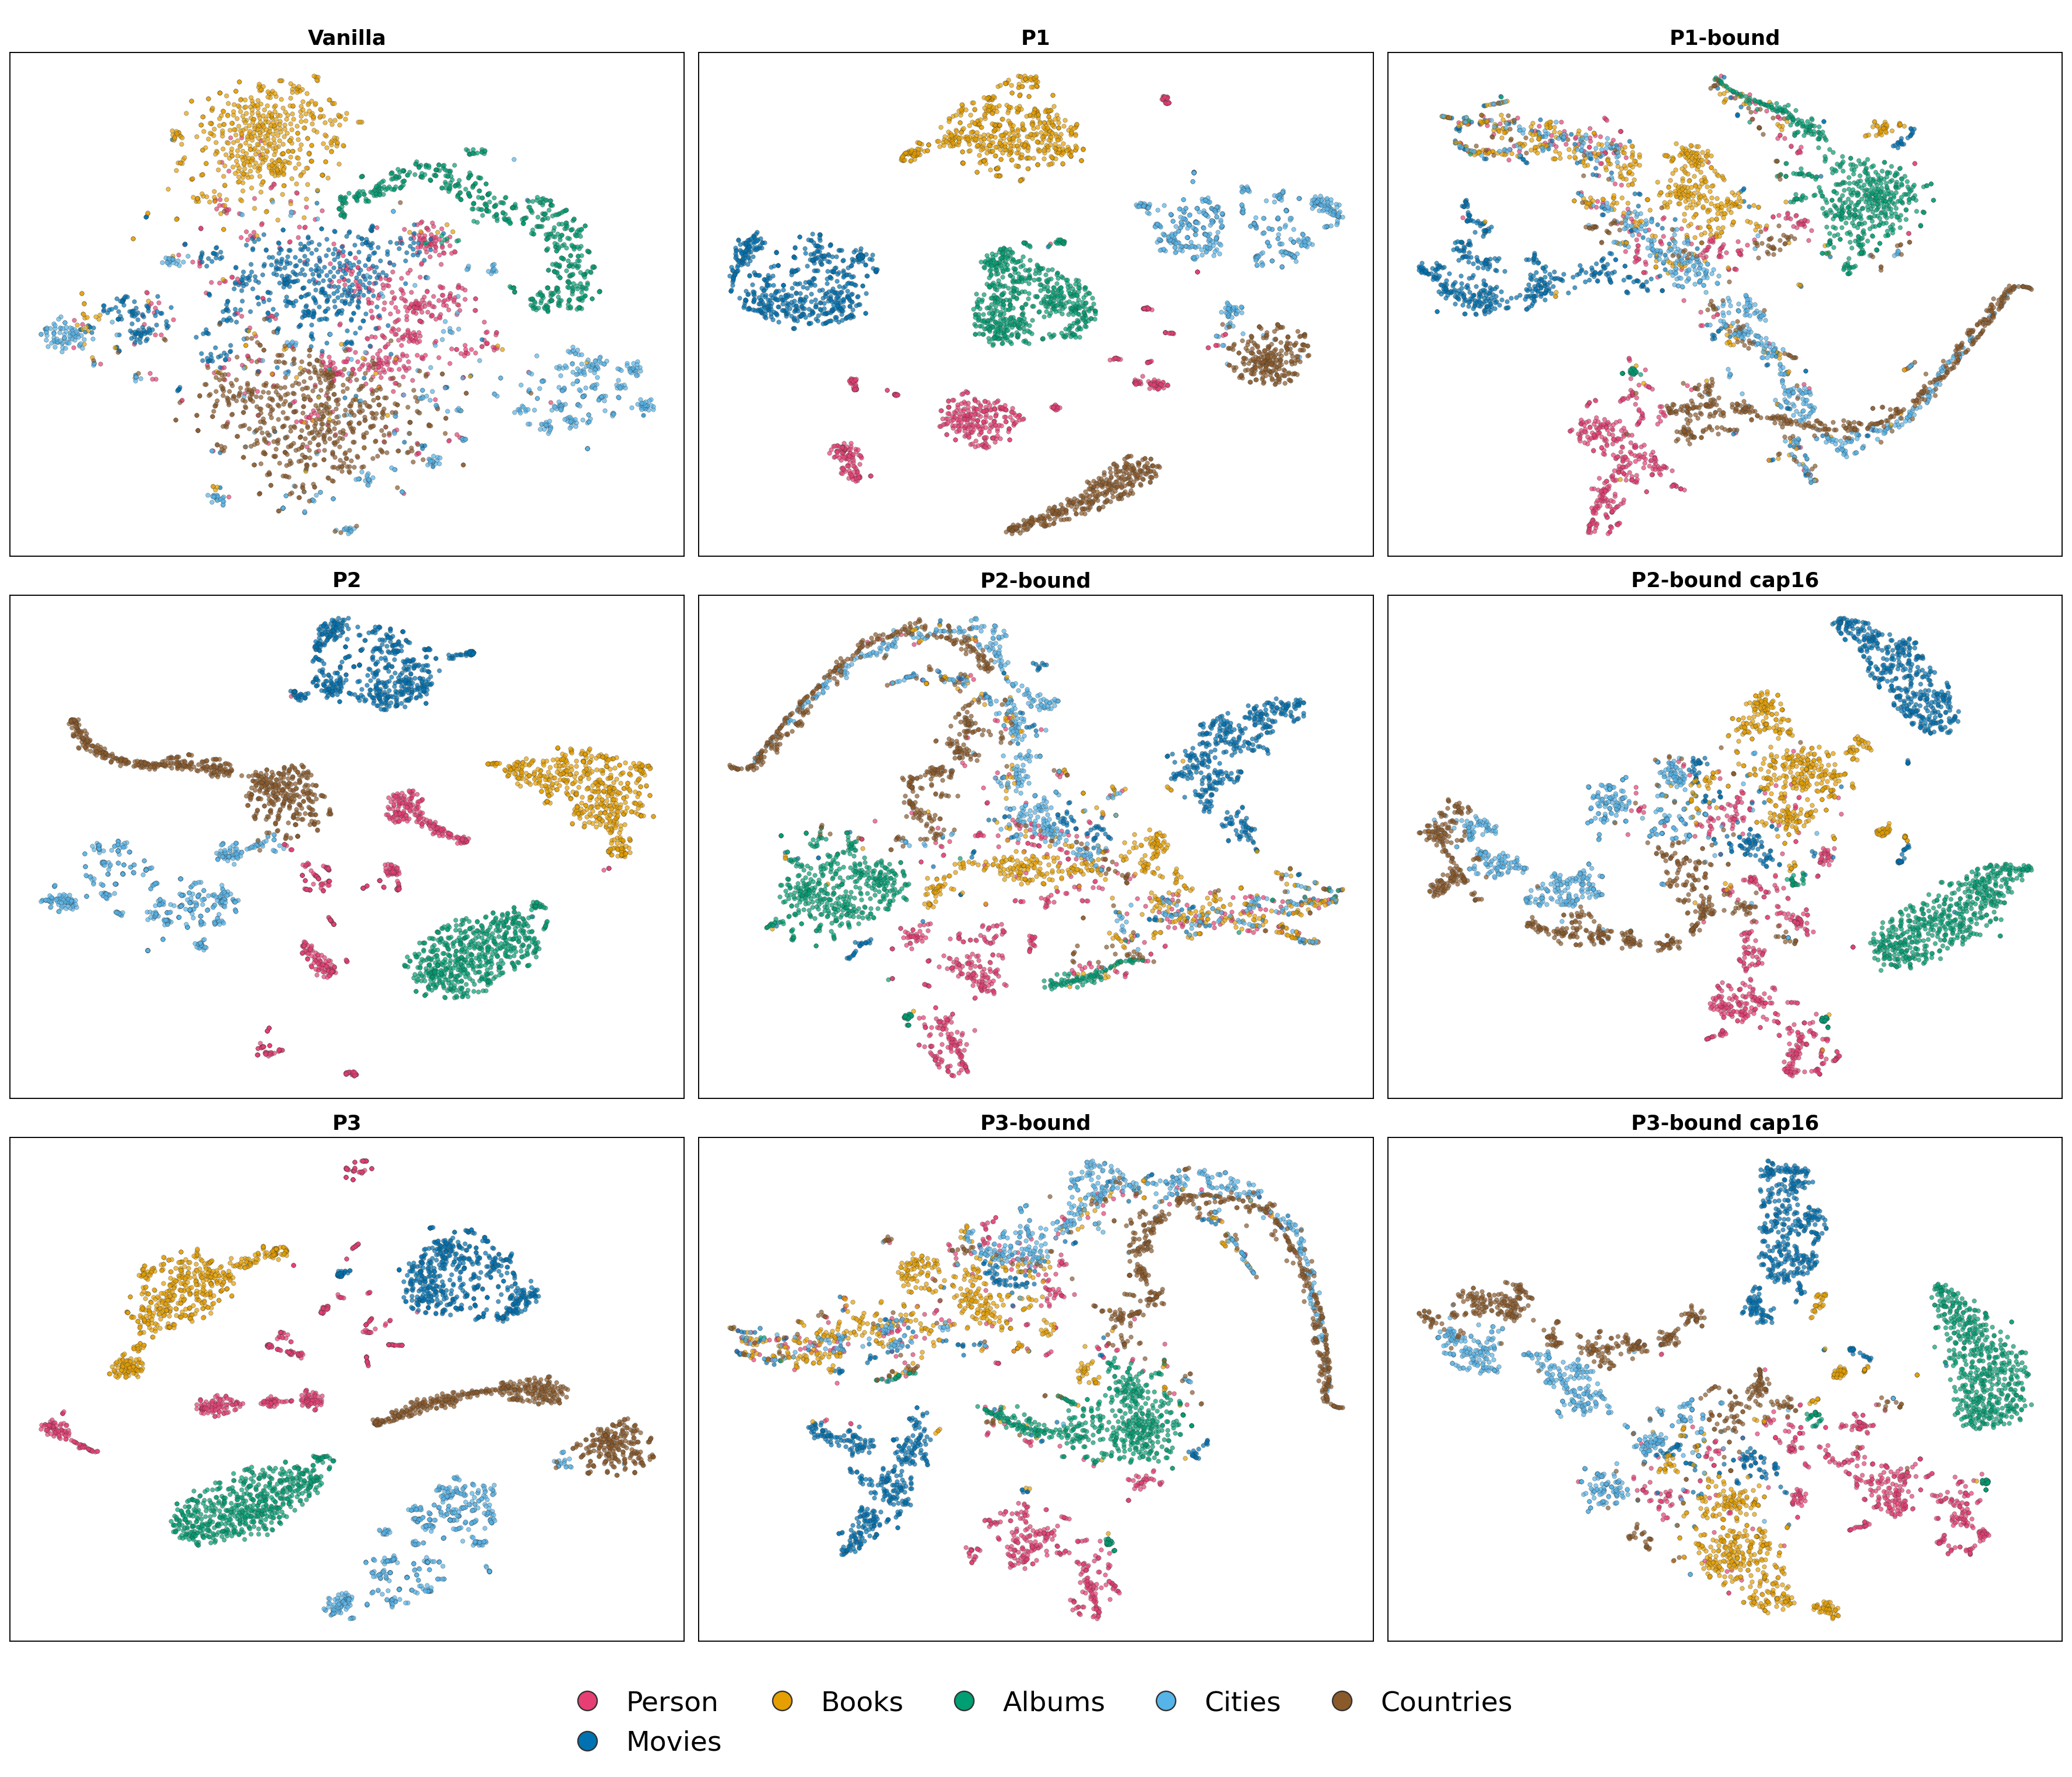
\includegraphics[width=\dimexpr\paperwidth-3cm\relax]{assets/dbpedia/pca_tsne_embedding_plot/dbpedia_schema_fine_tsne.png}}
      \caption{t-SNE}
      \label{fig:dbpedia_class_separation_tsne}
  \end{subfigure}
  \caption{Two-dimensional projections of the fine-tuned DBpedia entity
  embeddings, coloured by entity type (continued).}
\end{figure}

\section{Real-World Downstream Tasks (GEval)}
\label{sec:dbpedia_geval}

The DBpedia DLCC results above test the constructor families directly. To see
whether the same initializations help on standard downstream tasks, we evaluate
the fine-tuned DBpedia embeddings on the GEval
benchmark~\cite{pellegrino_configurable_2019,pellegrino_geval_2020}. Since the proposed methods target
schema-aware entity representations, we focus on the tasks where class structure
matters most: entity clustering, entity classification, and semantic analogies.
We compare \texttt{vanilla}, the classic transfer
(\texttt{p1}/\texttt{p2}/\texttt{p3}), and the norm-capped concept-bound init
(\texttt{cap16}). The uncapped bound is left out, because
Section~\ref{sec:dbpedia_class_separation} already shows that it is dominated by
its capped version. The plots are collected in Appendix~\ref{app:geval-plots}.

\paragraph{Clustering.} We run k-means on three GEval gold standards: CC and CCB
(cities vs.\ countries, which share the parent \texttt{dbo:Place}) and CAMAP
(five distinct classes), scored by adjusted Rand index (ARI;
Figure~\ref{fig:geval_clustering}). The classic transfer is the clear winner,
with ARI around $0.72$ on CC, $0.85$ on CCB, and up to $0.88$ on CAMAP, against
\texttt{vanilla} at $0.06$, $0.69$, and $0.78$. The gap is largest on the
shared-parent tasks (CC/CCB) and smallest on CAMAP, where co-occurrence already
separates the classes. The capped bound does not cluster well. It stays near the
\texttt{vanilla} floor on CC/CCB (ARI about $0.02$) and recovers only partly on
CAMAP. This matches the projections in
Section~\ref{sec:dbpedia_class_separation}, where the bound geometry trades class
compactness for relation information that k-means cannot read.

\paragraph{Classification.} The supervised task uses the entity embedding as
features and reports 10-fold cross-validated accuracy over a small classifier
panel (naive Bayes, $k$-NN, decision tree, linear SVM) on five datasets
(Figure~\ref{fig:geval_classification}). Once a classifier does the separating,
the variants flatten into a narrow band, with mean accuracy between about $0.46$
and $0.69$ and no clear winner. \texttt{vanilla} is competitive across all five
and best on Metacritic Movies (within $0.01$ of the top on Cities), while the
capped bound is best on others (AAUP, Forbes). The large classic-transfer advantage from clustering does not carry
over, because a fitted model recovers the class signal wherever the
initialization placed the points.

\paragraph{Semantic analogies.} As geometric evidence, we predict the fourth
entity of each quadruplet~\cite{mikolov_efficient_2013} with
3CosAdd~\cite{levy_linguistic_2014} and report top-1 accuracy on four relation
sets (Figure~\ref{fig:geval_analogies}). There is no single winner. The
classic transfer wins on the small capital-country set (top-1 $0.87$ vs.\
\texttt{vanilla} $0.68$) and on city-state, while \texttt{vanilla} wins on the
larger all-capital-country ($0.72$) and currency ($0.58$) sets. One reading is
that the classic init pulls every entity of a class toward one class code,
which helps coarse separation but blurs the detail needed to pick one specific
country out of many. The capped bound lands between the two.

Across the three tasks the same embeddings rank differently. The classic
transfer leads on clustering, flattens out on classification, and helps analogies
only at small scale, while the capped bound is weak on clustering but competitive
once a model or vector arithmetic reads it. The ranking from the synthetic DLCC
benchmark therefore does not carry over to real downstream tasks, and the best
initialization depends on the task.

\chapter{Discussion and Conclusions}
\label{ch:conclusion}
\label{sec:results_discussion}

Our contribution starts from adapting MASCHInE-style initialization to RDF2Vec.
RDF2Vec learns only from instance random walks and never reads the RDF schema.
MASCHInE showed that a schema can be compiled into a small protograph,
pre-trained, and transferred to initialize an instance model. It built this
recipe for link-prediction embeddings, not for RDF2Vec. We carry the idea to
RDF2Vec and ask a sharper question. Can the schema give RDF2Vec a useful starting
point, and what decides when it pays off?

To answer this we built two artifacts. The first is an RDF-schema view of DLCC.
It adds schema-specific test cases tc13--tc15 and the protograph constructions
P1, P2, and P3 that give every class a pre-trained code. The second is the
concept-bound initialization. It binds each entity to its (relation,
neighbour-class) pairs and to its direction-tagged edge counts. It then rescales
every vector to a shared target norm and fine-tunes at a protected rate, so the
transferred structure survives training. For comparison we use the classic
transfer (\texttt{most\_specific}), which only copies own-class vectors.

The thesis answers the question in two parts. The schema helps. But its value is
set by \emph{what} the initialization encodes, not by how much schema is
pre-trained. On a real graph a second condition appears. The gain survives only
if fine-tuning can still move what was encoded.

\paragraph{What the initialization must encode.} The relation-centric families
tc07--tc12 are where the schema should matter most. Vanilla RDF2Vec carries no
relation-specific signal there, and every classic variant stays in the same low
band, between $0.54$ and $0.73$. Copying own-class vectors adds nothing when the
target is a relation rather than a class. The concept-bound initialization changes
this. Its best variant lifts the mean on these families by $0.28$ over vanilla.
The gain is not learning. The bound signal is already linearly readable at the
first epoch, and the protected fine-tuning keeps it. So it is an initialization
effect. The classic transfer has a narrow reach by design. It copies own-class
vectors and nothing more. It therefore helps only where the label \emph{is} the
own class, which on the synthetic suite is the single test case tc14. Each
initialization wins exactly where its encoded content matches the task.

\paragraph{Why the win does not survive on a real graph, and the one-line fix.}
On DBpedia the picture inverts. After five epochs over 89 splits the uncapped
concept-bound finishes worst end-to-end, below both vanilla and every classic
variant, and the classic transfer leads. The cause is visible before any instance
training. At epoch~0 the concept-bound already reads the schema, scoring a mean
of $0.769$ against a vanilla chance level of $0.500$. The cost sits in the same
mechanism. The cardinality channel writes edge counts into vector magnitude. A
few high-degree hubs then reach norms of about $65{,}000$. A protected step cannot
turn vectors that large, so those rows freeze. The very channel that builds the
head start prevents fine-tuning from moving it. The fix is one line. Capping the
norm on those few thousand rows turns the worst variant into the best overall
($0.808 \rightarrow 0.850$ on the standardize lens) and leads on the hard splits.
Reshaping the class
\emph{content} instead, by specificity or hierarchy weighting, moves individual
splits but cancels in the aggregate. On a real graph the end-to-end result is
governed by the magnitude of the init, not by its schema content. The schema
still has to be movable for fine-tuning to keep it.

\paragraph{Which initialization to pick in practice.} The DLCC ranking does not
carry over to standard downstream tasks. On GEval the best initialization depends
on the task. Clustering rewards the classic transfer most clearly, with adjusted
Rand index of $0.72$--$0.88$ across the three gold standards; its margin over
vanilla is largest on the shared-parent tasks (vanilla $0.06$ on CC, $0.69$ on
CCB) and smallest on CAMAP (vanilla $0.78$), while the capped bound
clusters poorly. Classification flattens everyone into a narrow band with no clear
winner, because a fitted model recovers the class signal wherever the
initialization placed the points. Analogies are mixed. So a high DLCC score does
not predict downstream quality. The right initialization is a task-level choice.

\paragraph{What bounds these claims.} Several limits bound the conclusions. The
synthetic generator decorrelates each constructor from degree and popularity by
design. The synthetic gains therefore read as an upper bound, not as a forecast
for real graphs. The DBpedia account is a diagnosis, not a controlled
one-factor-at-a-time decomposition. The cap comparisons run on a $10\%$
sub-corpus, though the full corpus reproduces the headline. The shared target
norm of $8$, the cap of $16$, and the uniform term coefficients were fixed rather
than jointly swept. Finally, the differences are noisy. On synthetic data, gaps
below roughly three points are ties, and on DBpedia gaps within the
$\approx\!0.003$ standard deviation of the capped runs are ties. A few ablations
rest on a single seed.

Taken together, the results give one coherent answer. Schema-based pre-training
can give RDF2Vec a useful starting point. The concept-bound construction is what
makes the relation-centric targets reachable at all, because it writes the bound
pairs and edge counts that the classic transfer cannot reach. What decides the
payoff is the content of the encoding on a clean benchmark, and the movability of
that content on a real graph. The cardinality channel earns the head start and
then locks it in place, and a single norm cap is enough to free it. On a rich real
corpus the headroom is small, because most of the benchmark signal is already
available for free. There the practical contribution narrows to one cheap and
robust component. A per-row norm cap keeps a schema-bound initialization from
freezing and lets it stay competitive end-to-end on a real knowledge graph.

\section{Future Work}
\label{sec:future_work}

Several directions remain open. The anchoring and noise ablations
(Sections~\ref{sec:anchoring} and~\ref{sec:jitter}) were each evaluated in
isolation. Anchoring pulls only the class-initialized instances back toward
their schema-informed vectors, the noise is added on top of the classic and
concept-bound initializations, and the two were never combined. Neither control
touched the randomly initialized instances. Whether anchoring helps when paired
with random-noise initialization, for instance by anchoring noise-perturbed or
randomly initialized embeddings rather than only the class-initialized ones, is
left to future work.

The shared target norm is a second untested choice. Once a vector has been
assembled for every instance, the whole set is rescaled by a single global
scalar so that the mean instance norm equals \texttt{TARGET\_NORM} $= 8$
(Section~\ref{sec:norm}), a value kept fixed in all experiments but never
ablated. Why $8$ rather than some other length, and how strongly the target
norm affects the saturation of the RDF2Vec sigmoid and the resulting retention
of transferred structure during fine-tuning, should be measured empirically. We
leave a sweep over the shared target norm to future work.

On DBpedia the end-to-end gap of the concept-bound construction is accounted for
by a diagnosis rather than a decomposition: we did not run a controlled ablation
that isolates each contributing cause on the real graph
(Section~\ref{sec:dbpedia_diagnosis}). A dedicated experiment that varies one
factor at a time, such as the available headroom, the degree-shaped benchmark
mass, and the coverage of the protograph, would turn that diagnosis into a
quantitative attribution. We leave such a controlled real-graph ablation to
future work.

The DBpedia comparisons also run on a reduced training corpus. To hold the
amount of training data fixed and keep the compute tractable, the cap and the
count-compression, cap-size, and learning-rate ablations all use the $10\%$
sub-corpus of 116M tokens (Section~\ref{sec:dbpedia_cap}). These runs are stable.
The repeated-run variation is small (Appendix~\ref{app:stability-analysis}), and
the full corpus reproduces the headline result. Even so, the absolute numbers
would be more precise if every comparison were rerun end-to-end on the full
corpus. We leave a full-corpus replication of the DBpedia ablations to future
work.

The concept-bound construction keeps the coefficients of its four terms uniform,
so that each term's contribution can be isolated
(Equation~\eqref{eq:bound_init}). Tuning these coefficients, for instance to
up-weight whichever concept type a downstream task relies on, was not explored
and is left to future work.

Finally, the hierarchy-climbing coverage strategies reach full initialization
coverage but do not improve final accuracy over \texttt{most\_specific}
(Section~\ref{sec:results_init_strategies}). We attribute this to over-smoothing,
where sharing a common ancestor vector collapses instances that were previously
distinct, but we did not measure the effect directly. Confirming the
over-smoothing explanation, for example by quantifying how initialization
diversity shrinks as coverage is filled, is left to future work.

\bibliography{references}


\appendix

\section{Vocabulary Initialization Coverage}
\label{app:vocab-coverage}

Table~\ref{tab:vocab_init_coverage_tc01_tc15} reports the full vocabulary-level
initialization coverage for P1, P2, and P3 across all DLCC Synthetic test cases,
referenced from Section~\ref{sec:coverage}.

\begin{table}[ht]
\centering
\small
\caption{Vocabulary initialization coverage for P1, P2, and P3 on DLCC Synthetic test cases TC01--TC15. \emph{Init} reports protograph-initialized tokens out of the full vocabulary size; \emph{Ent} and \emph{Rel} are initialized entity and relation tokens; \emph{Rand} is the number of randomly initialized tokens. The P1/P2 columns for TC01--TC12 are the originally reported figures; the P3 column and the TC13--TC15 rows are recomputed from the synthetic-benchmark checkpoints, whose vocabulary sizes may differ from the original P1/P2 runs by up to four tokens and whose relation counts reflect full protograph-walk coverage.}
\label{tab:vocab_init_coverage_tc01_tc15}
\resizebox{\textwidth}{!}{%
\begin{tabular}{lcccccccccccc}
\toprule
\multirow{2}{*}{\textbf{TC}}
& \multicolumn{4}{c}{\textbf{P1}}
& \multicolumn{4}{c}{\textbf{P2}}
& \multicolumn{4}{c}{\textbf{P3}} \\
\cmidrule(lr){2-5}
\cmidrule(lr){6-9}
\cmidrule(lr){10-13}
& \textbf{Init} & \textbf{Ent} & \textbf{Rel} & \textbf{Rand}
& \textbf{Init} & \textbf{Ent} & \textbf{Rel} & \textbf{Rand}
& \textbf{Init} & \textbf{Ent} & \textbf{Rel} & \textbf{Rand} \\
\midrule
TC01 & 6392/10920 (58.5\%) & 5544 & 848 & 4528 & 9465/10920 (86.7\%) & 8525 & 940 & 1455 & 10917/10917 (100.0\%) & 9975 & 942 & 0 \\
TC02 & 6519/10927 (59.7\%) & 5670 & 849 & 4408 & 9778/10927 (89.5\%) & 8839 & 939 & 1149 & 10924/10924 (100.0\%) & 9981 & 943 & 0 \\
TC03 & 6323/10932 (57.8\%) & 5493 & 830 & 4609 & 9578/10932 (87.6\%) & 8636 & 942 & 1354 & 10932/10932 (100.0\%) & 9988 & 944 & 0 \\
TC04 & 84059/119338 (70.4\%) & 82936 & 1123 & 35279 & 111383/119338 (93.3\%) & 110174 & 1209 & 7955 & 119334/119334 (100.0\%) & 118118 & 1216 & 0 \\
TC05 & 8681/12990 (66.8\%) & 7740 & 941 & 4309 & 11789/12990 (90.8\%) & 10754 & 1035 & 1201 & 12990/12990 (100.0\%) & 11953 & 1037 & 0 \\
TC06 & 6176/10932 (56.5\%) & 5335 & 841 & 4756 & 9126/10932 (83.5\%) & 8183 & 943 & 1806 & 10932/10932 (100.0\%) & 9987 & 945 & 0 \\
TC07 & 7023/12845 (54.7\%) & 6186 & 837 & 5822 & 11497/12845 (89.5\%) & 10566 & 931 & 1348 & 12845/12845 (100.0\%) & 11912 & 933 & 0 \\
TC08 & 6780/10920 (62.1\%) & 5931 & 849 & 4140 & 9765/10920 (89.4\%) & 8838 & 927 & 1155 & 10920/10920 (100.0\%) & 9990 & 930 & 0 \\
TC09 & 7849/13548 (57.9\%) & 6960 & 889 & 5699 & 12045/13548 (88.9\%) & 11063 & 982 & 1503 & 13548/13548 (100.0\%) & 12565 & 983 & 0 \\
TC10 & 7203/12498 (57.6\%) & 6342 & 861 & 5295 & 10862/12498 (86.9\%) & 9913 & 949 & 1636 & 12498/12498 (100.0\%) & 11547 & 951 & 0 \\
TC11 & 6639/11873 (55.9\%) & 5783 & 856 & 5234 & 10344/11873 (87.1\%) & 9386 & 958 & 1529 & 11873/11873 (100.0\%) & 10913 & 960 & 0 \\
TC12 & 6196/15927 (38.9\%) & 5341 & 855 & 9731 & 12557/15927 (78.8\%) & 11598 & 959 & 3370 & 15927/15927 (100.0\%) & 14966 & 961 & 0 \\
TC13 & 11972/19702 (60.8\%) & 10976 & 996 & 7730 & 16904/19702 (85.8\%) & 15908 & 996 & 2798 & 19702/19702 (100.0\%) & 18706 & 996 & 0 \\
TC14 & 14955/17913 (83.5\%) & 13965 & 990 & 2958 & 17604/17913 (98.3\%) & 16614 & 990 & 309 & 17913/17913 (100.0\%) & 16923 & 990 & 0 \\
TC15 & 13783/19213 (71.7\%) & 12773 & 1010 & 5430 & 18857/19213 (98.1\%) & 17847 & 1010 & 356 & 19213/19213 (100.0\%) & 18203 & 1010 & 0 \\
\bottomrule
\end{tabular}%
}
\end{table}

\section{Repeated-Run Stability Analysis of RDF2Vec}
\label{app:stability-analysis}

To estimate the run-to-run variation of the RDF2Vec-based experiments, we repeated three configurations (\texttt{vanilla}, \texttt{p1\_classic}, and \texttt{p2\_classic}) five times each, on eleven test cases (\texttt{tc01}--\texttt{tc03} and \texttt{tc05}--\texttt{tc12}). \texttt{tc04} is excluded because its instance-walk corpus is about fifteen times larger than the others, which makes five repeated end-to-end runs prohibitively slow; the schema-specific cases \texttt{tc13}--\texttt{tc15} are absent because they had not yet been introduced when this stability study was run. To measure the variation fairly, each repetition is an independent end-to-end sample: it regenerates its own random-walk corpus with a different walk seed \emph{and} varies the Word2Vec/protograph training seed, while the train/test splits are held fixed. The estimate therefore reflects walk-sampling variance in addition to training randomness, rather than training randomness alone. The results are reported in Table~\ref{tab:stability-five-runs} and visualised in Figure~\ref{fig:stability-fluctuation}.

\begin{figure}[ht]
\centering
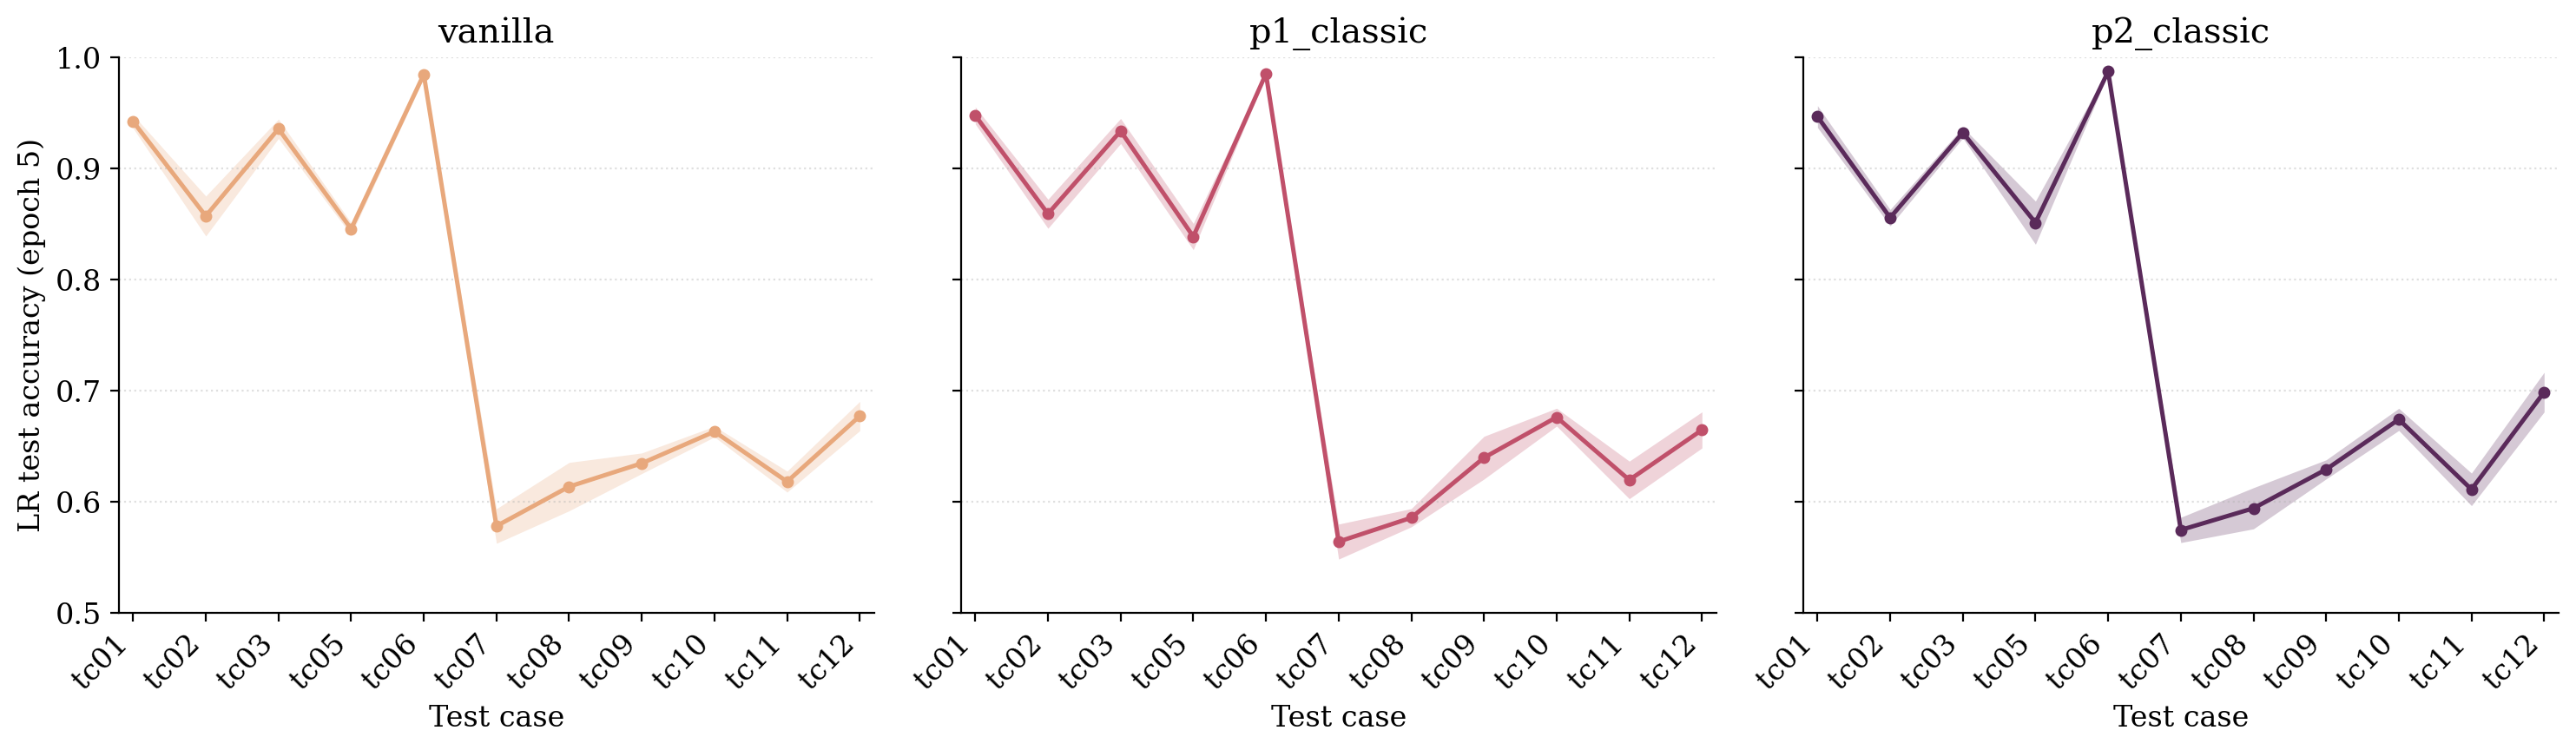
\includegraphics[width=\linewidth]{assets/stability_ribbon.png}
\caption{Per-test-case mean final Logistic Regression test accuracy over five repeated RDF2Vec runs, one panel per variant. Each run resamples its own walk corpus and varies the training seed; shaded bands show $\pm 1$ standard deviation across the five runs. The narrow bands indicate low run-to-run fluctuation even when walk-sampling variance is included.}
\label{fig:stability-fluctuation}
\end{figure}

\begin{table}[ht]
\centering
\caption{Stability analysis of final Logistic Regression test accuracy over five repeated RDF2Vec runs. Each run regenerates its own random-walk corpus (different walk seed) and varies the Word2Vec/protograph training seed; the train/test splits are held fixed. Values are reported as mean $\pm$ standard deviation over five runs.}
\label{tab:stability-five-runs}
\begin{tabular}{lccc}
\toprule
\textbf{Test case} & \textbf{Vanilla} & \textbf{P1-classic} & \textbf{P2-classic} \\
\midrule
tc01 & $0.942 \pm 0.006$ & $0.948 \pm 0.008$ & $0.947 \pm 0.010$ \\
tc02 & $0.857 \pm 0.018$ & $0.859 \pm 0.013$ & $0.855 \pm 0.007$ \\
tc03 & $0.935 \pm 0.009$ & $0.934 \pm 0.011$ & $0.932 \pm 0.005$ \\
tc05 & $0.846 \pm 0.005$ & $0.839 \pm 0.012$ & $0.851 \pm 0.019$ \\
tc06 & $0.985 \pm 0.003$ & $0.985 \pm 0.002$ & $0.987 \pm 0.002$ \\
tc07 & $0.578 \pm 0.016$ & $0.564 \pm 0.016$ & $0.575 \pm 0.011$ \\
tc08 & $0.613 \pm 0.022$ & $0.586 \pm 0.008$ & $0.594 \pm 0.019$ \\
tc09 & $0.634 \pm 0.009$ & $0.639 \pm 0.019$ & $0.629 \pm 0.009$ \\
tc10 & $0.663 \pm 0.005$ & $0.676 \pm 0.008$ & $0.674 \pm 0.010$ \\
tc11 & $0.618 \pm 0.009$ & $0.620 \pm 0.017$ & $0.611 \pm 0.015$ \\
tc12 & $0.677 \pm 0.013$ & $0.665 \pm 0.016$ & $0.699 \pm 0.018$ \\
\midrule
Mean std. & $0.0105$ & $0.0118$ & $0.0113$ \\
Max std. & $0.0218$ & $0.0192$ & $0.0194$ \\
\bottomrule
\end{tabular}
\end{table}

We use this study to define a noise floor for the single-seed main results
(Section~\ref{sec:results_synthetic}). Because each repetition re-samples its
walk corpus in addition to varying the training seed, the estimate captures both
the variance of the random-walk sampling and that of Word2Vec training (only the
train/test splits are held fixed); it is therefore a more complete estimate of
run-to-run noise than one obtained by re-using a single fixed walk corpus. The
average standard deviation of the final Logistic Regression accuracy is $0.0112$,
and the maximum across all tested configurations is $0.0218$ (tc08,
\texttt{vanilla}); on the easiest cases (e.g.\ tc06) it is around $0.002$.
Notably, adding walk-sampling variance leaves the noise essentially unchanged
relative to an otherwise identical fixed-walk analysis ($0.0106$ mean / $0.0272$
max), confirming that the RDF2Vec results are robust to the particular walk
corpus drawn and that the run-to-run variation is dominated by training
stochasticity. Since the main results report a single run per variant, we take a
conservative round-up of the largest observed standard deviation and treat
differences below approximately three percentage points as within the observed
variation; gains only slightly above this threshold are interpreted cautiously.
In short, the run-to-run noise is at most ${\approx}2$--$3$ percentage points
(worst case: ${\approx}2.2$ pp with walk resampling, ${\approx}2.7$ pp fixed-walk),
and we treat any difference below ${\approx}3$ percentage points as within noise
to be safe.
The variation shrinks as $1/\sqrt{n}$ with the number of repeated runs, so
resolving sub-percentage-point effects would require substantially more than five
runs per configuration.



\section{Label-Aware (LDA) Class Distribution for All Synthetic Test Cases}
\label{app:lda-all}

This appendix shows label-aware Linear Discriminant Analysis (LDA) projections of
the entity embeddings for the DLCC synthetic test cases (tc01 to tc08 and tc10 to
tc12). Each panel projects one method's test entities onto its first linear
discriminant (LD1), the label-aware axis motivated in
Section~\ref{sec:results_diagnostics}, where we also explain why a variance-based
PCA projection can hide the label boundary (on tc07, \texttt{p3\_bound} is
separable at $0.99$ accuracy yet looks mixed under PCA). Under this view the
\texttt{p3\_bound} variant separates the positive and negative entities, whereas
\texttt{vanilla} and the classic variants remain mixed even on the axis chosen to
separate them, which corroborates their near-chance accuracies on the
relation-centric tasks.

\begin{center}
  \captionsetup{type=figure}
  \captionof{figure}{LDA (label-aware) projections of entity embeddings for the
  DLCC synthetic test cases (tc01 to tc08 and tc10 to tc12), taken after full
  training (5 pretraining epochs for P1/P2, followed by 5 fine-tuning epochs).
  Each panel projects one method's test entities onto its first linear
  discriminant (LD1, horizontal) and first principal component (PC1, vertical).}
  \label{fig:lda_appendix}

  \begin{longtable}{c}
  \makebox[\linewidth][c]{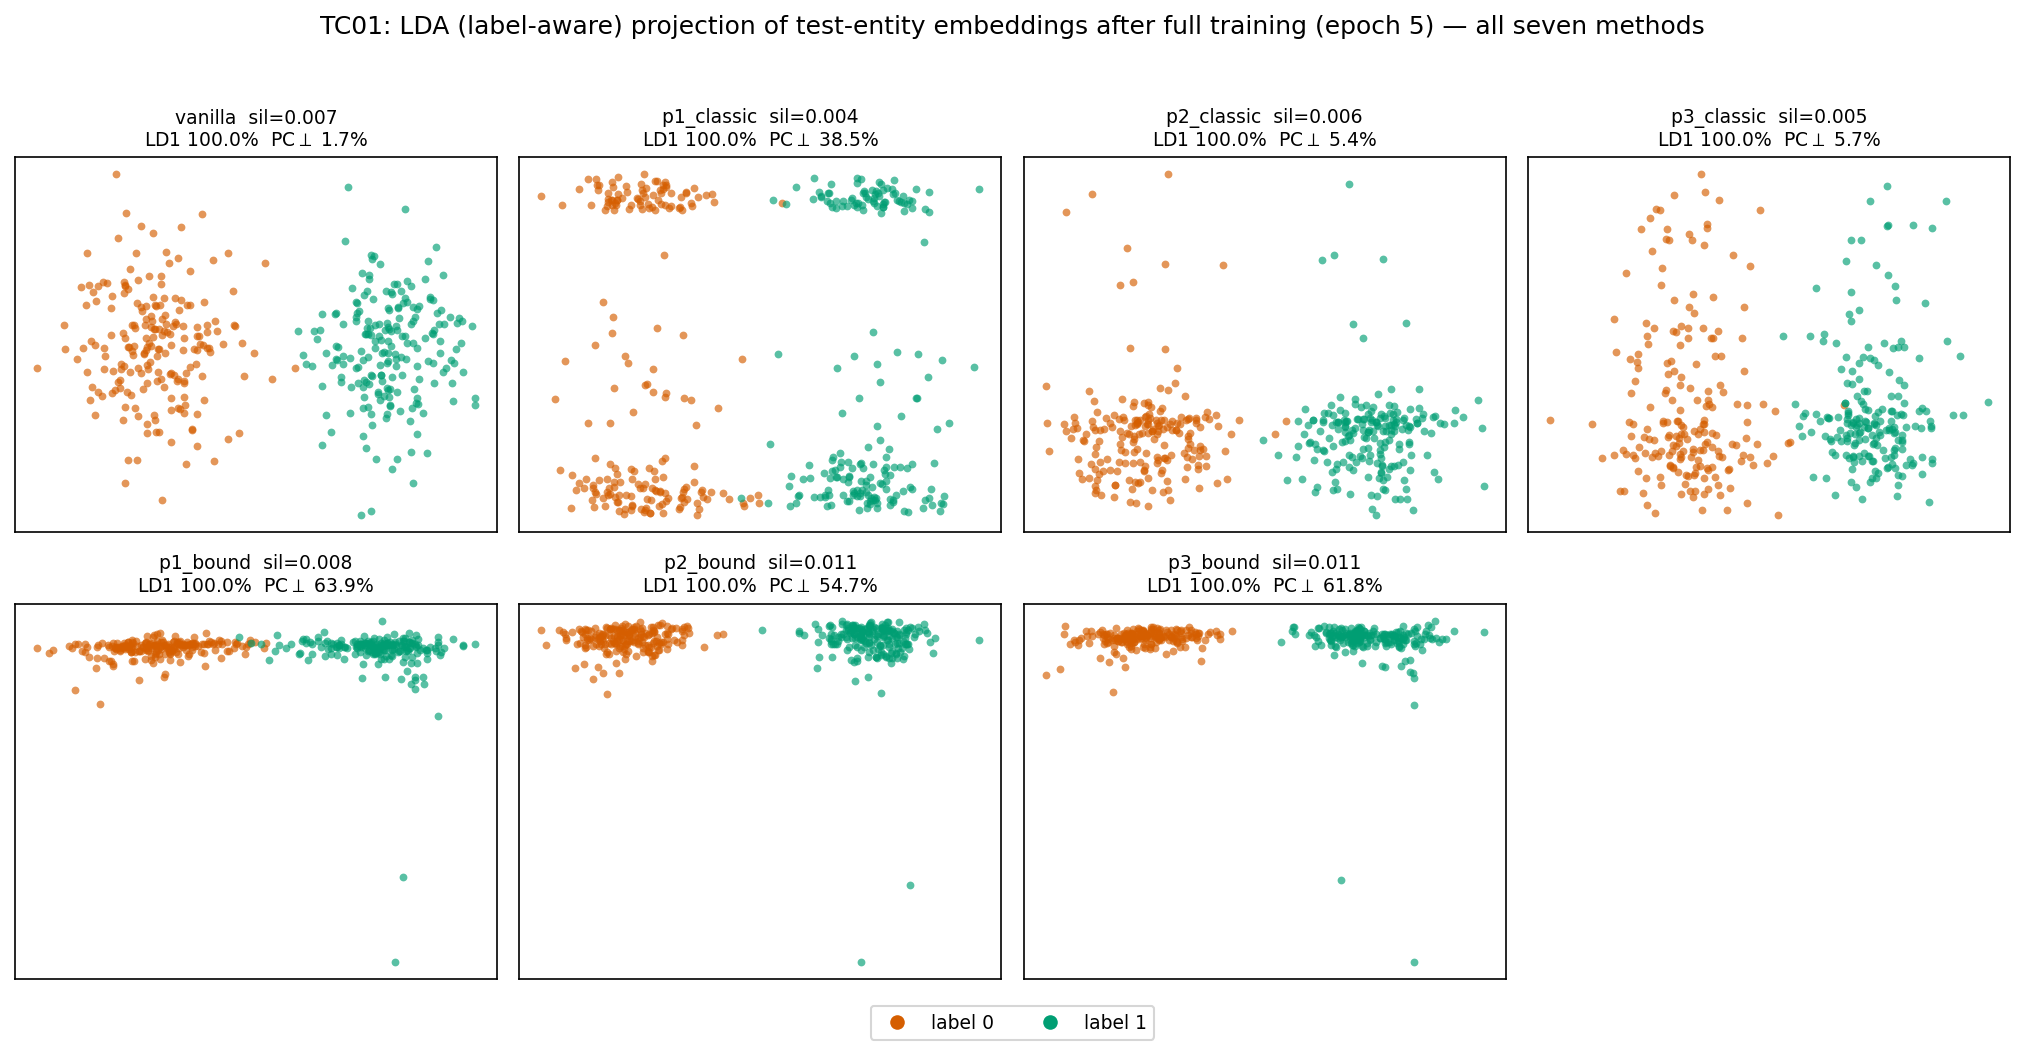
\includegraphics[width=\dimexpr\paperwidth-3cm\relax]{assets/lda/tc01_lda.png}} \\[1.0em]

  \makebox[\linewidth][c]{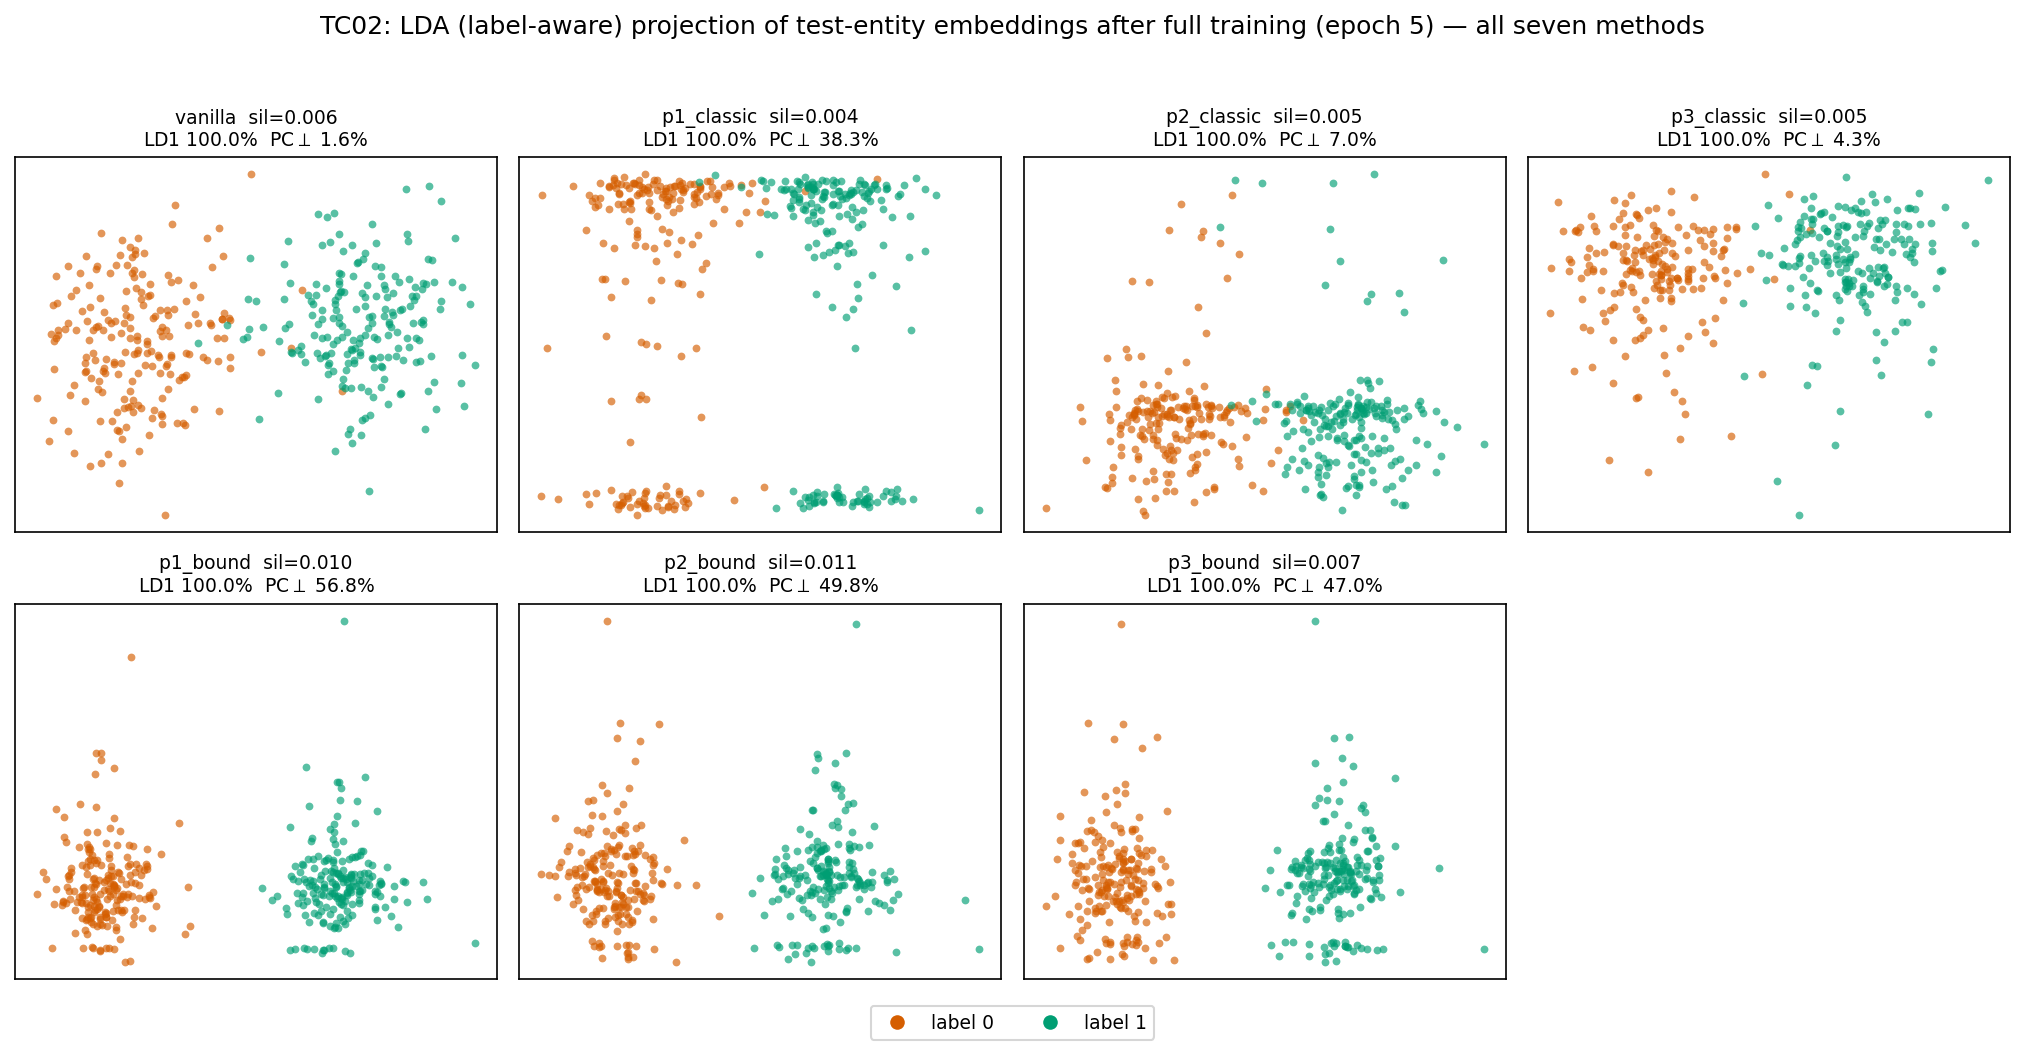
\includegraphics[width=\dimexpr\paperwidth-3cm\relax]{assets/lda/tc02_lda.png}} \\[1.0em]

  \makebox[\linewidth][c]{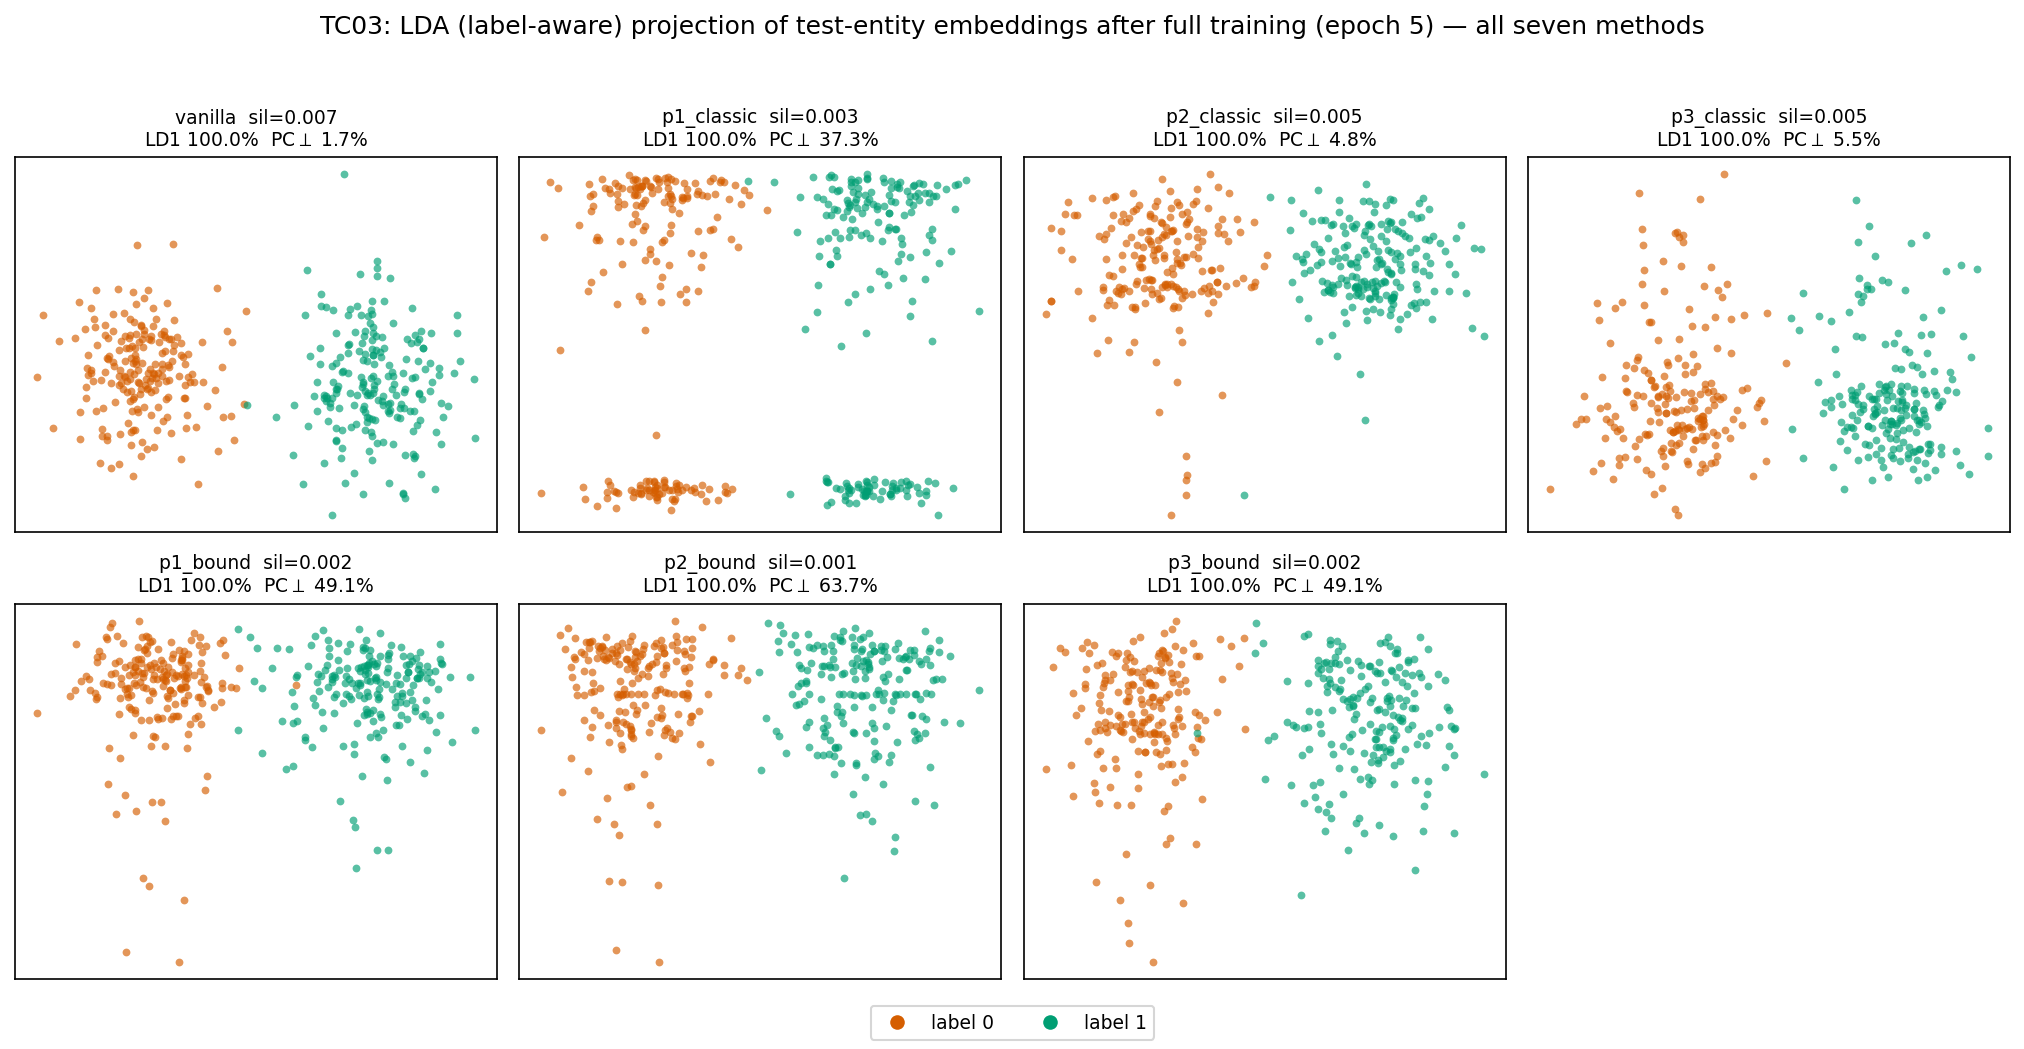
\includegraphics[width=\dimexpr\paperwidth-3cm\relax]{assets/lda/tc03_lda.png}} \\[1.0em]

  \makebox[\linewidth][c]{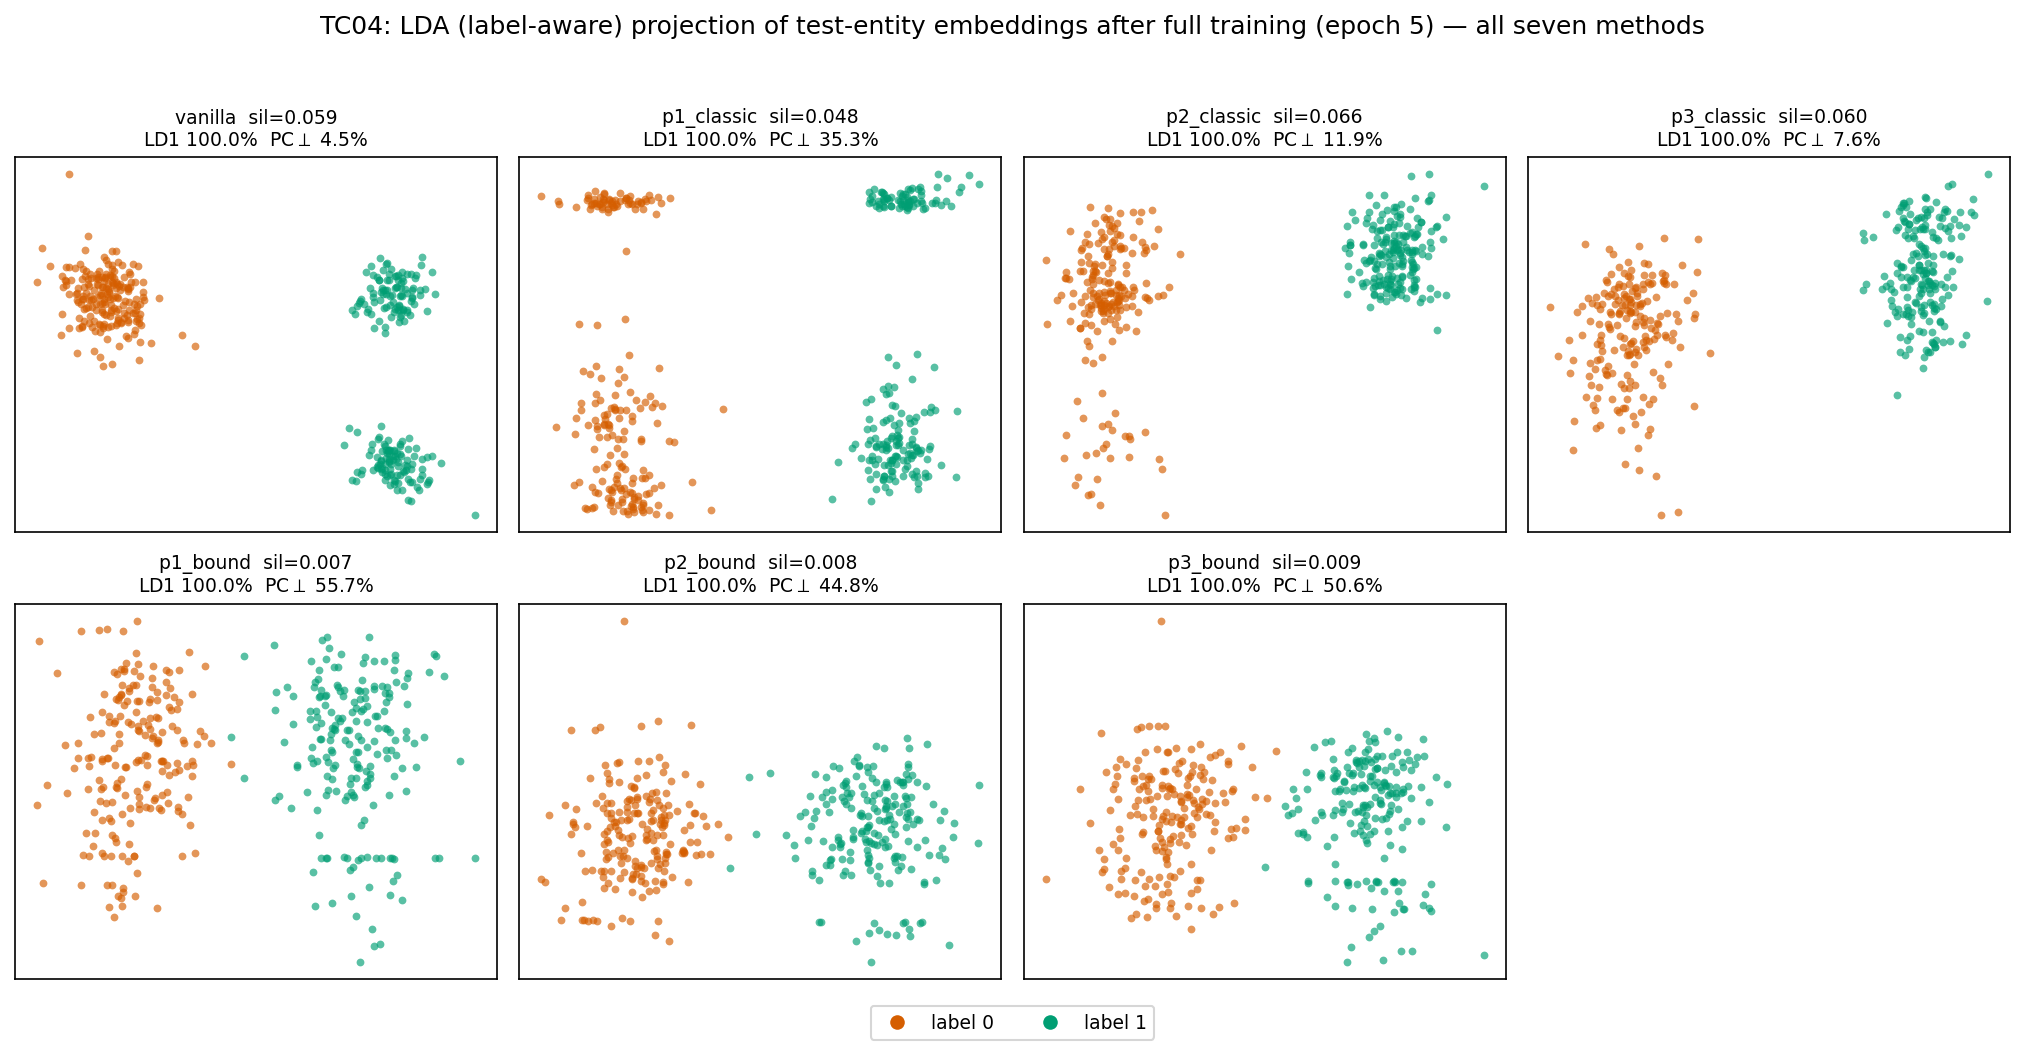
\includegraphics[width=\dimexpr\paperwidth-3cm\relax]{assets/lda/tc04_lda.png}} \\[1.0em]

  \makebox[\linewidth][c]{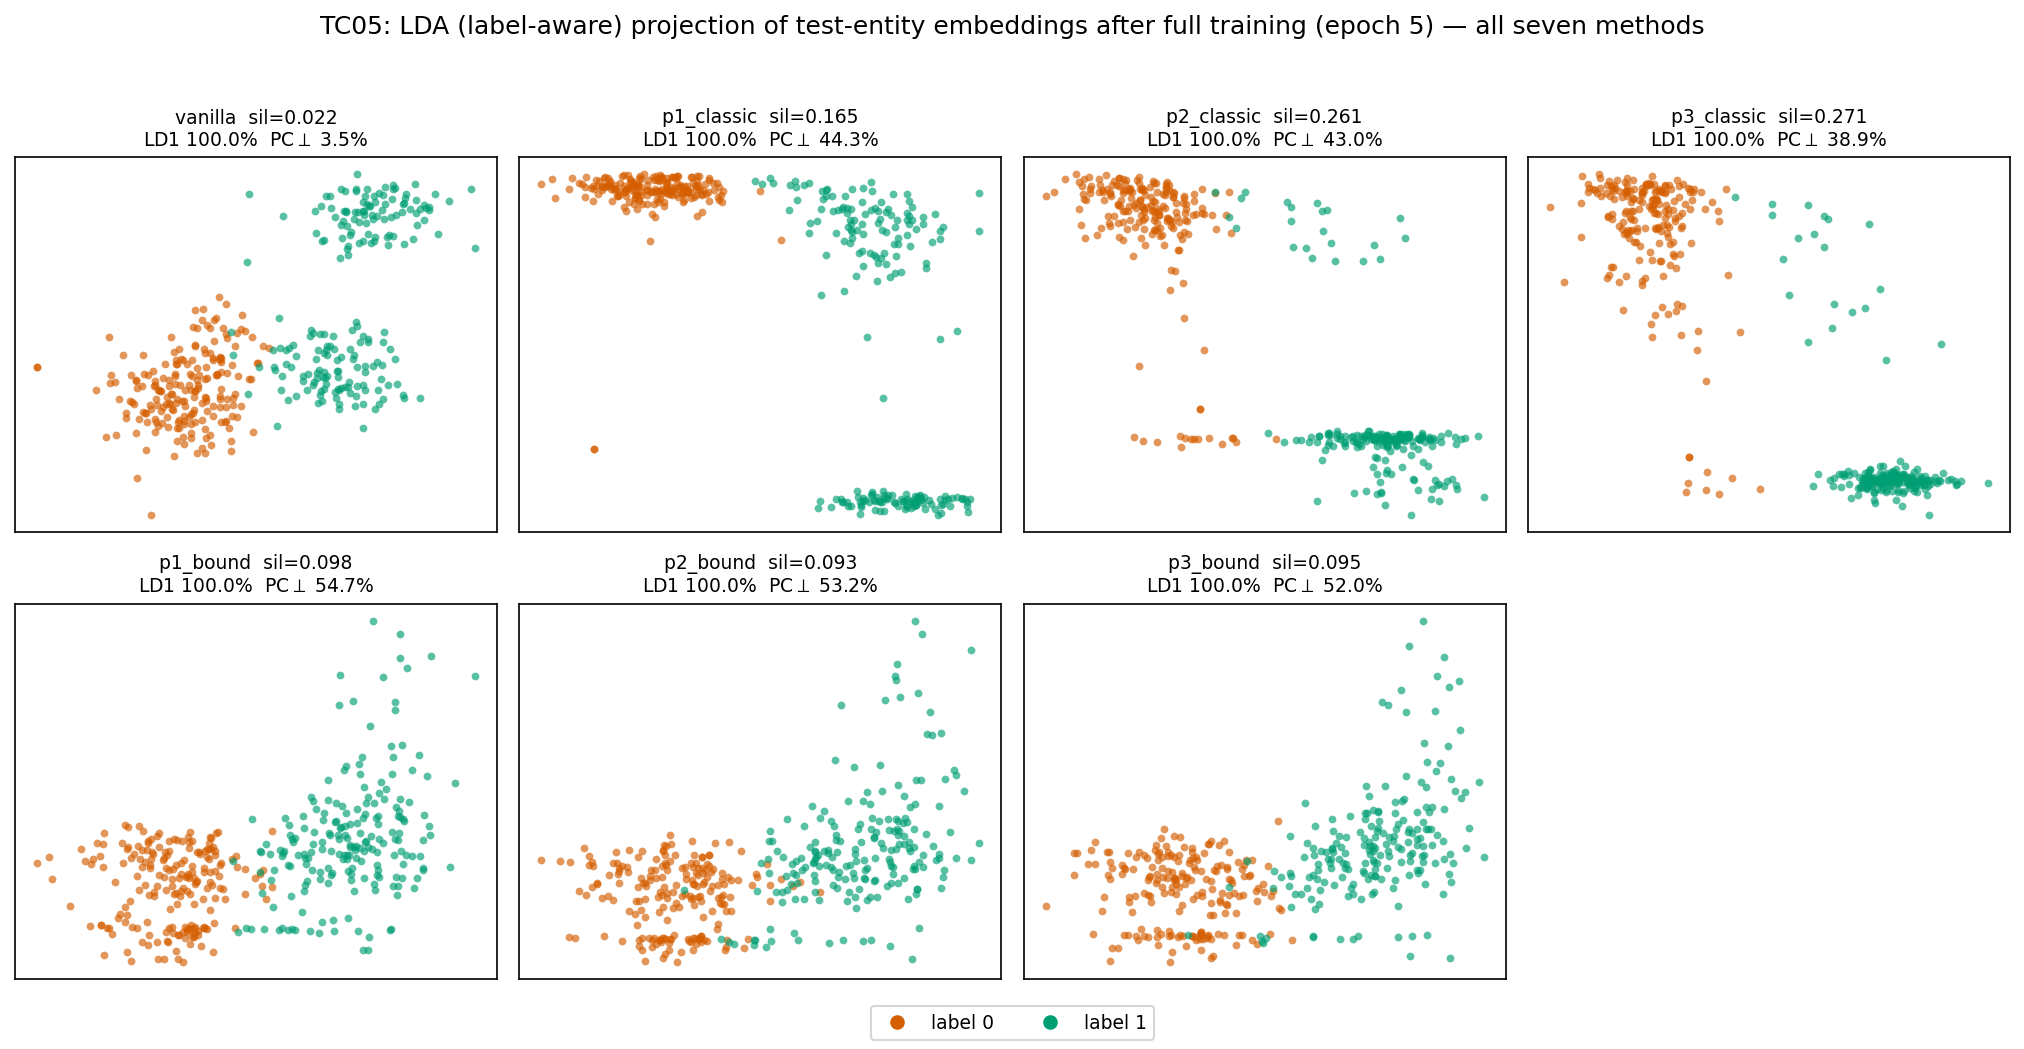
\includegraphics[width=\dimexpr\paperwidth-3cm\relax]{assets/lda/tc05_lda.png}} \\[1.0em]

  \makebox[\linewidth][c]{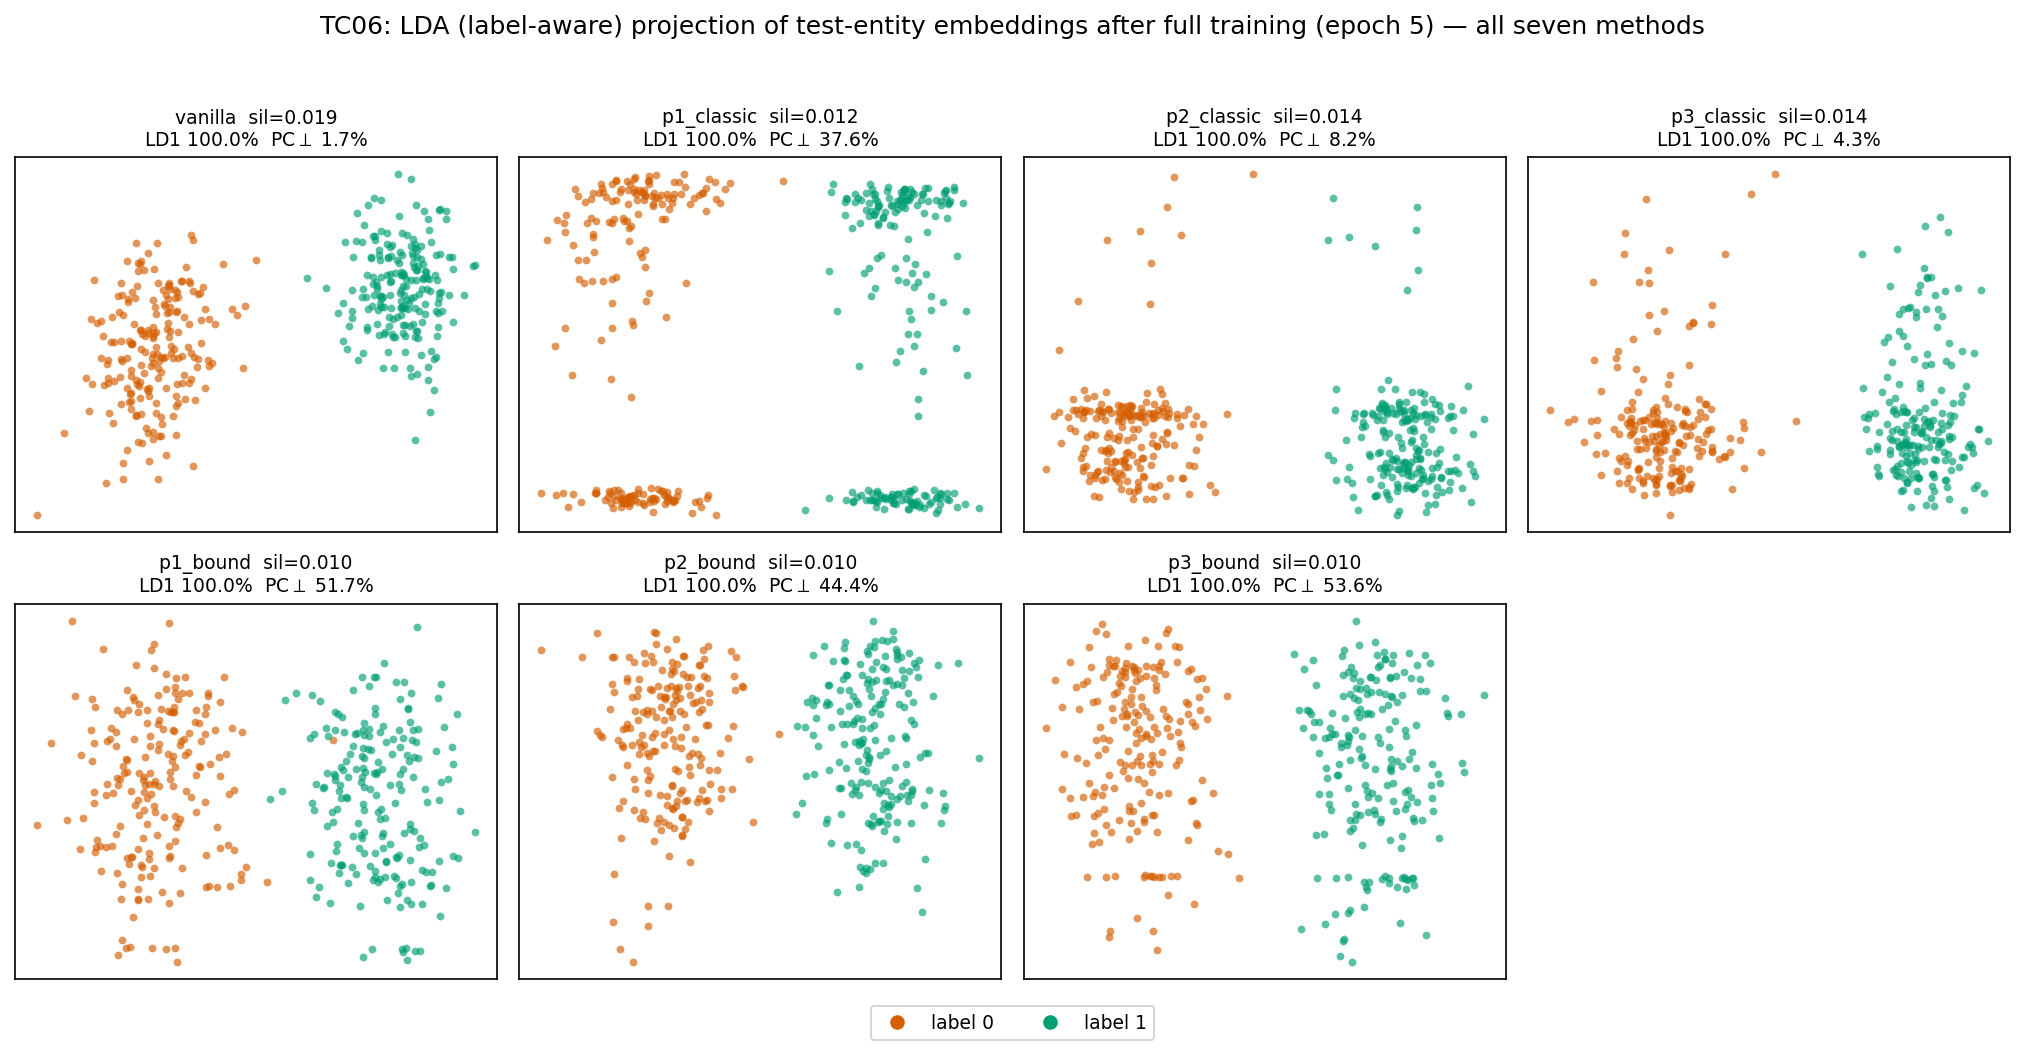
\includegraphics[width=\dimexpr\paperwidth-3cm\relax]{assets/lda/tc06_lda.png}} \\[1.0em]

  \makebox[\linewidth][c]{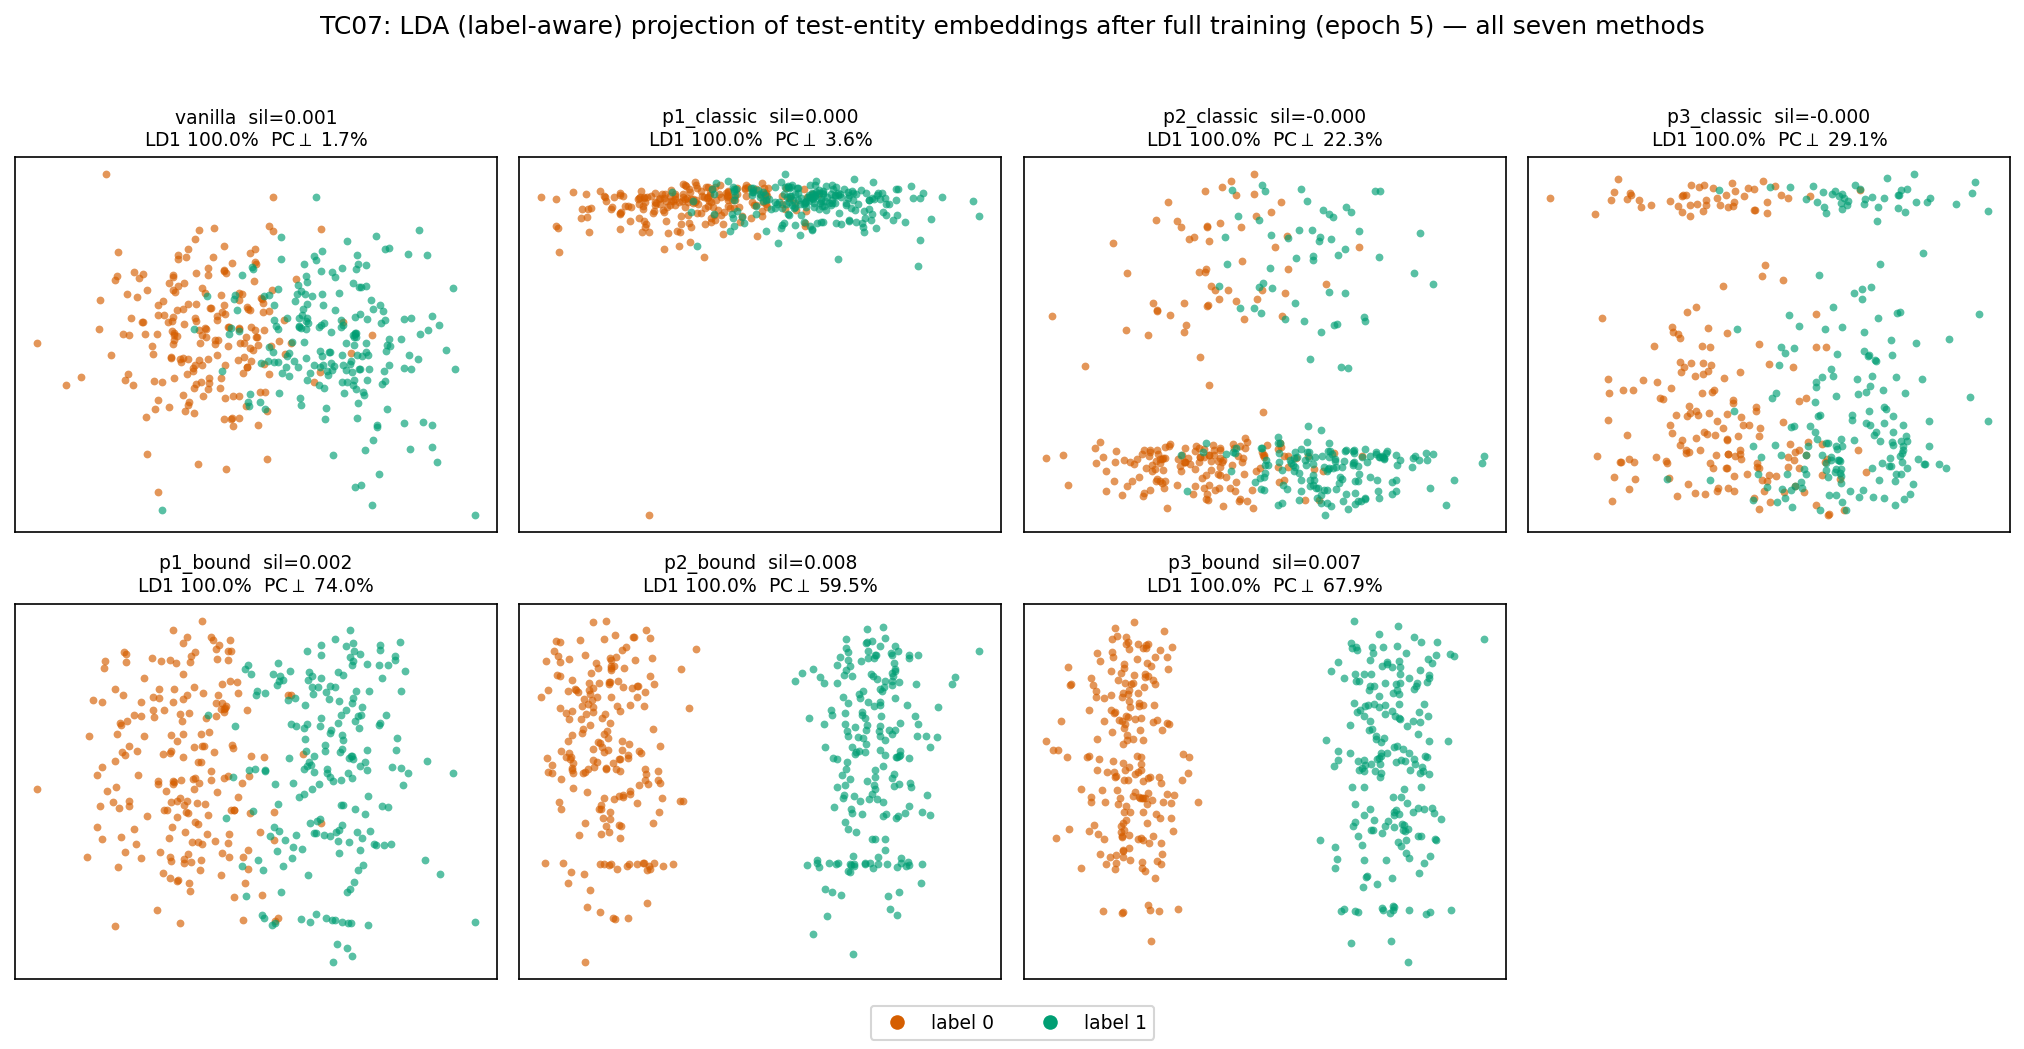
\includegraphics[width=\dimexpr\paperwidth-3cm\relax]{assets/lda/tc07_lda.png}} \\[1.0em]

  \makebox[\linewidth][c]{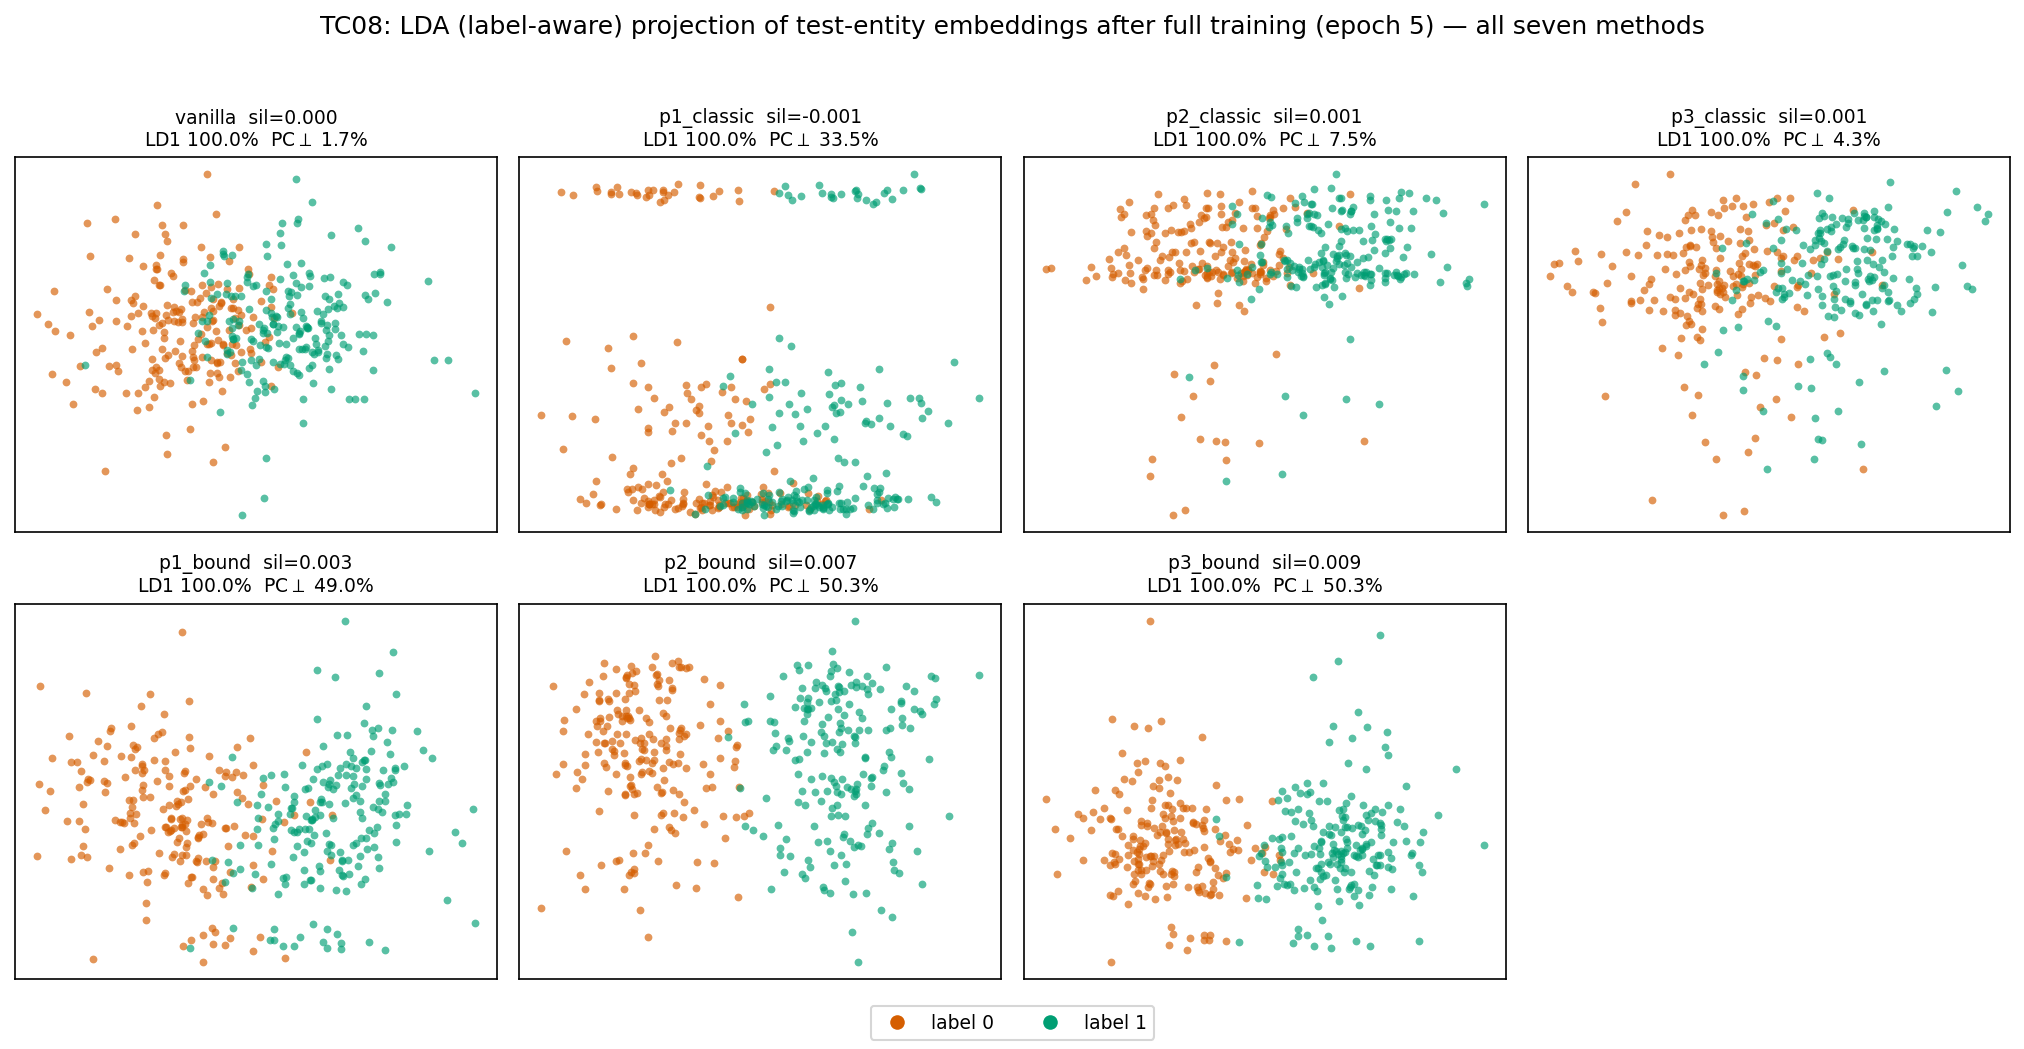
\includegraphics[width=\dimexpr\paperwidth-3cm\relax]{assets/lda/tc08_lda.png}} \\[1.0em]

  \makebox[\linewidth][c]{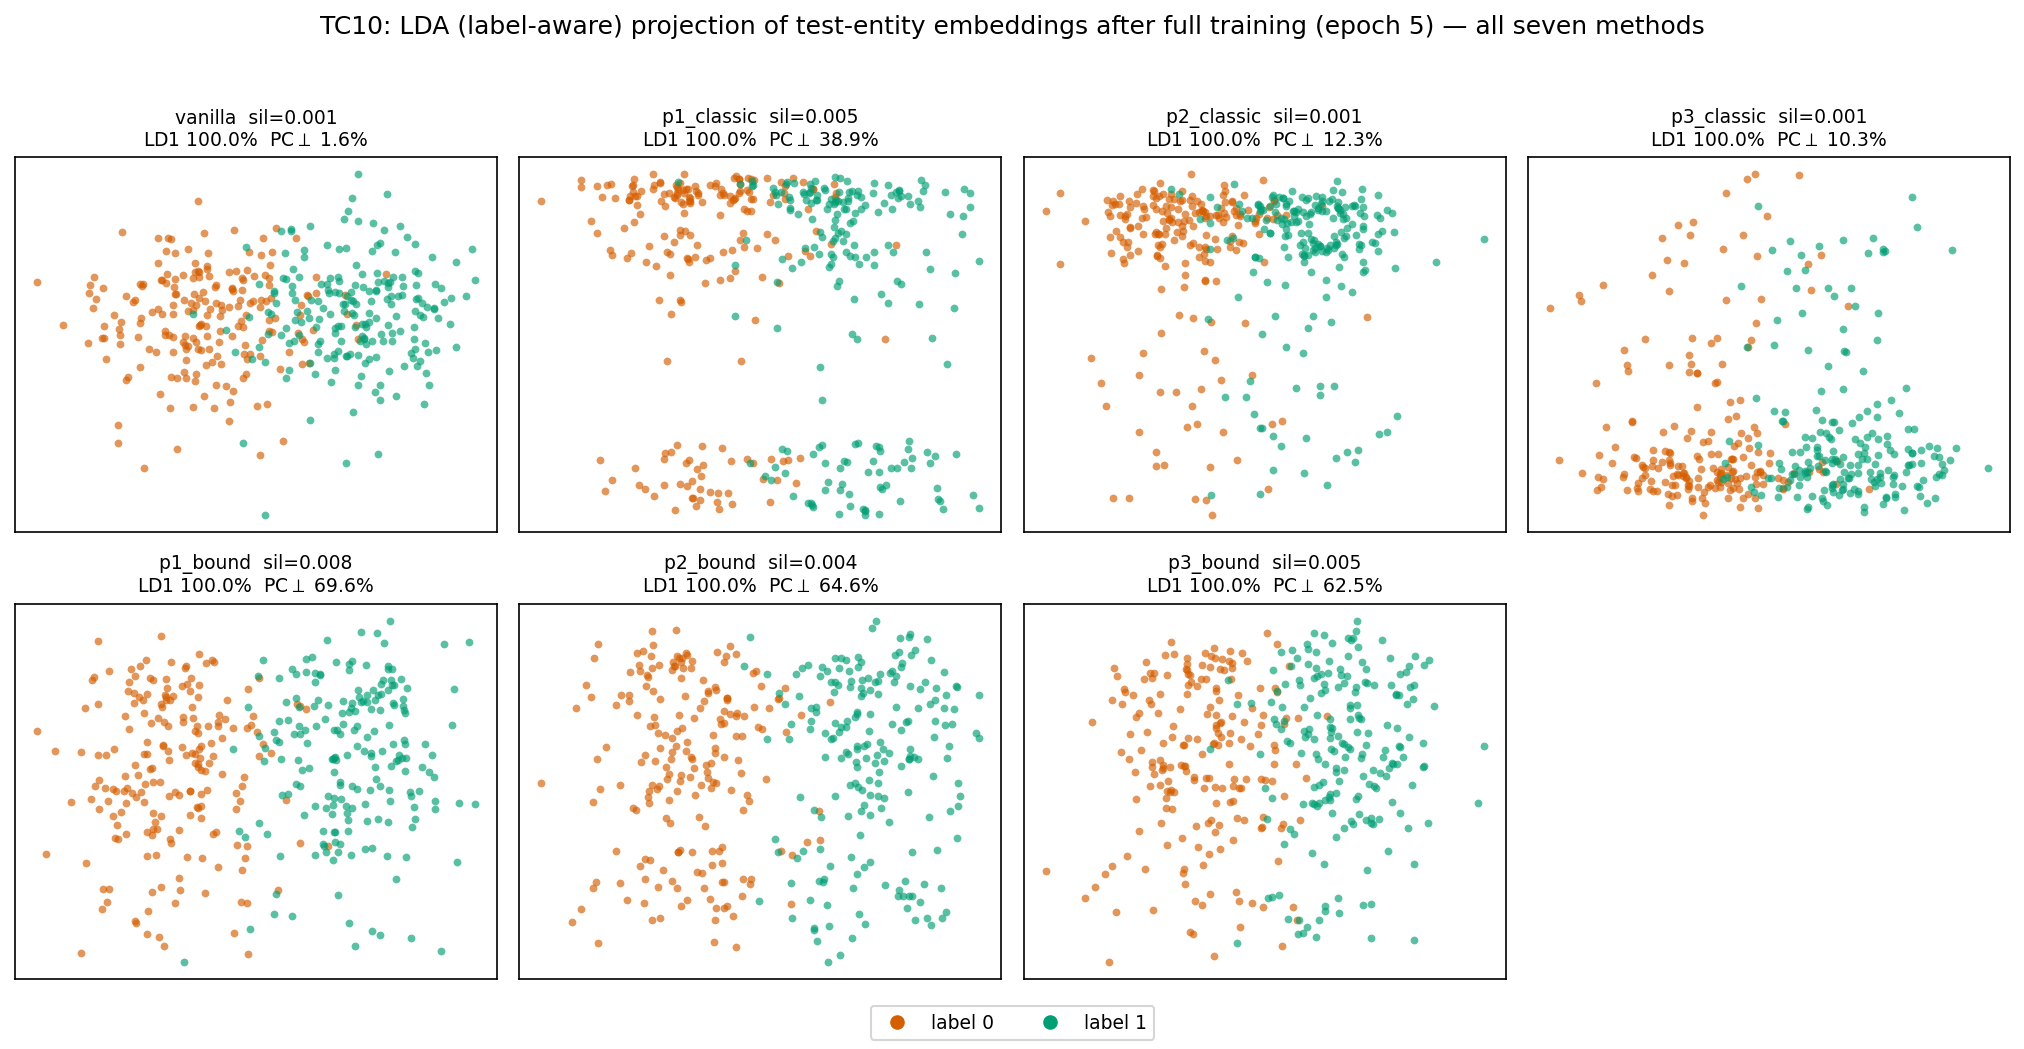
\includegraphics[width=\dimexpr\paperwidth-3cm\relax]{assets/lda/tc10_lda.png}} \\[1.0em]

  \makebox[\linewidth][c]{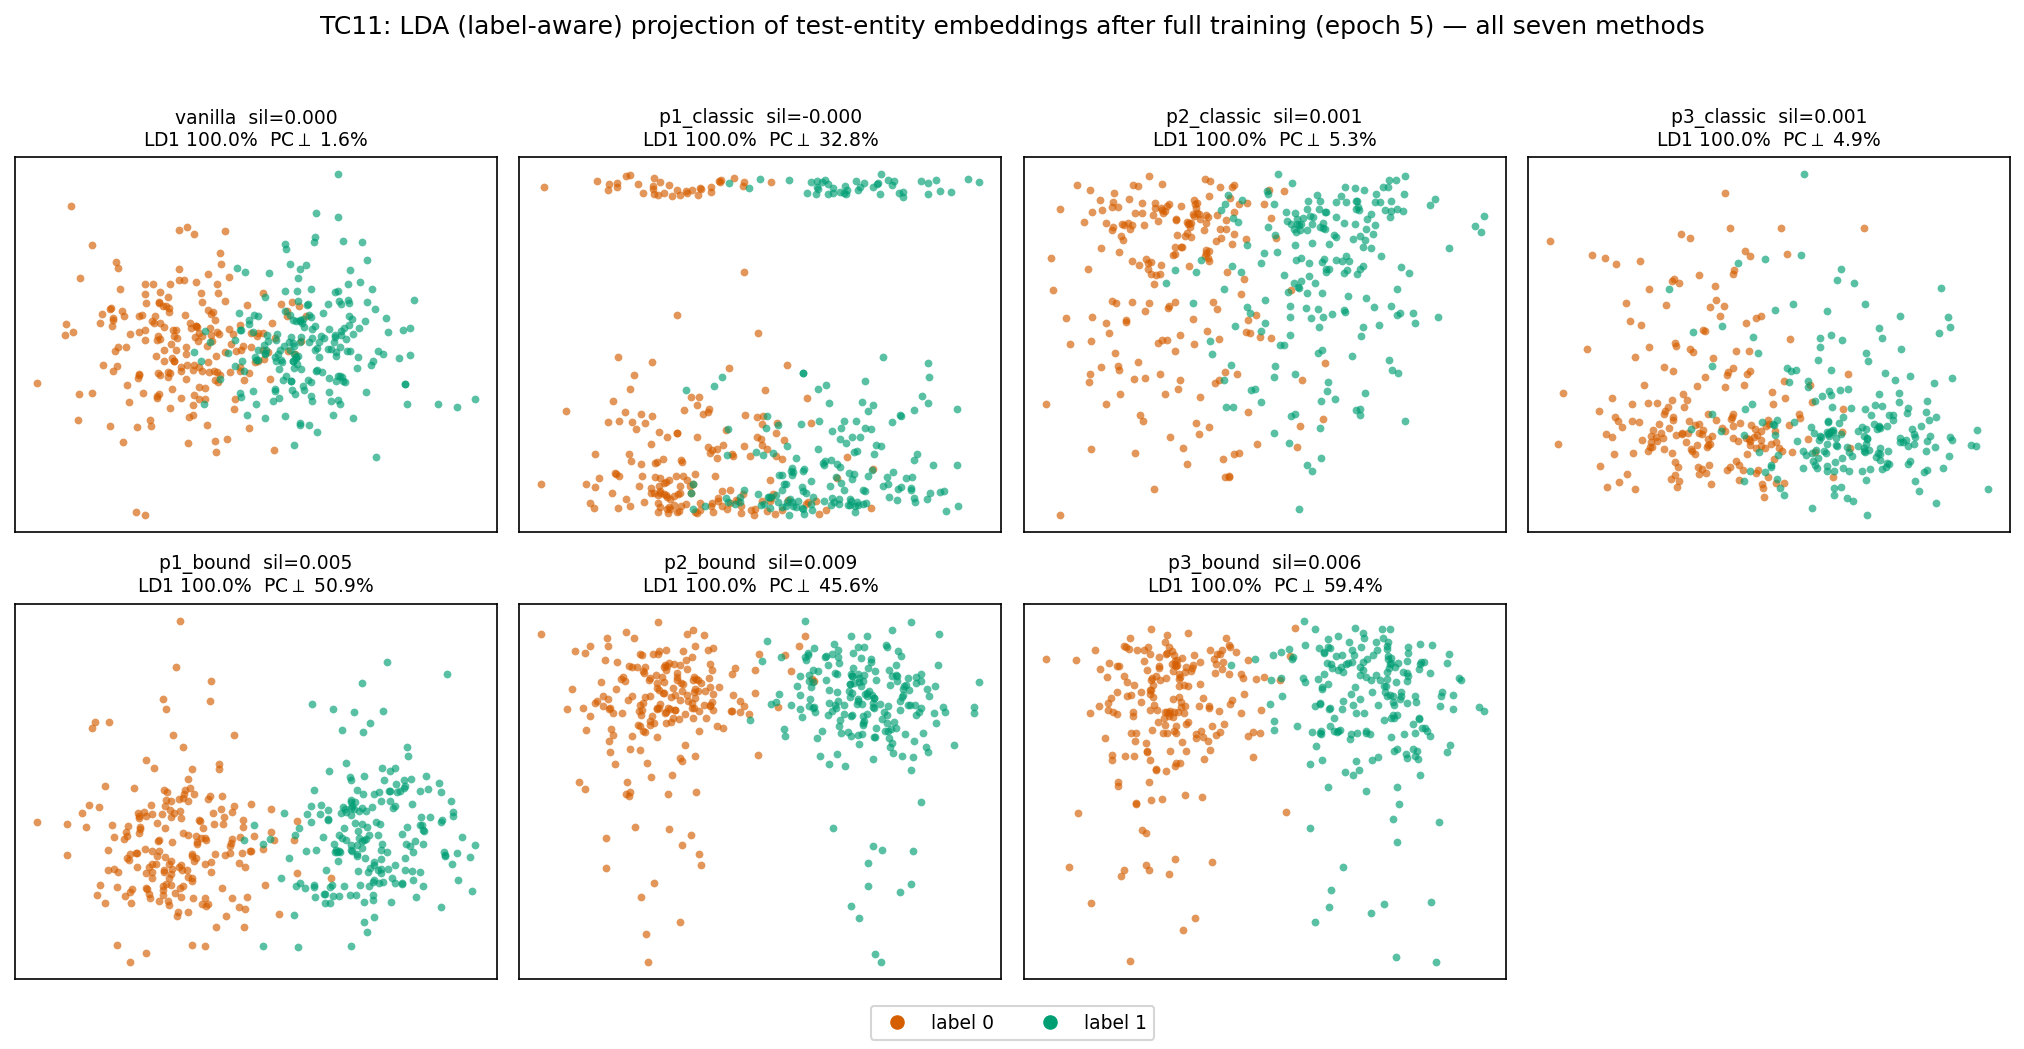
\includegraphics[width=\dimexpr\paperwidth-3cm\relax]{assets/lda/tc11_lda.png}} \\[1.0em]

  \makebox[\linewidth][c]{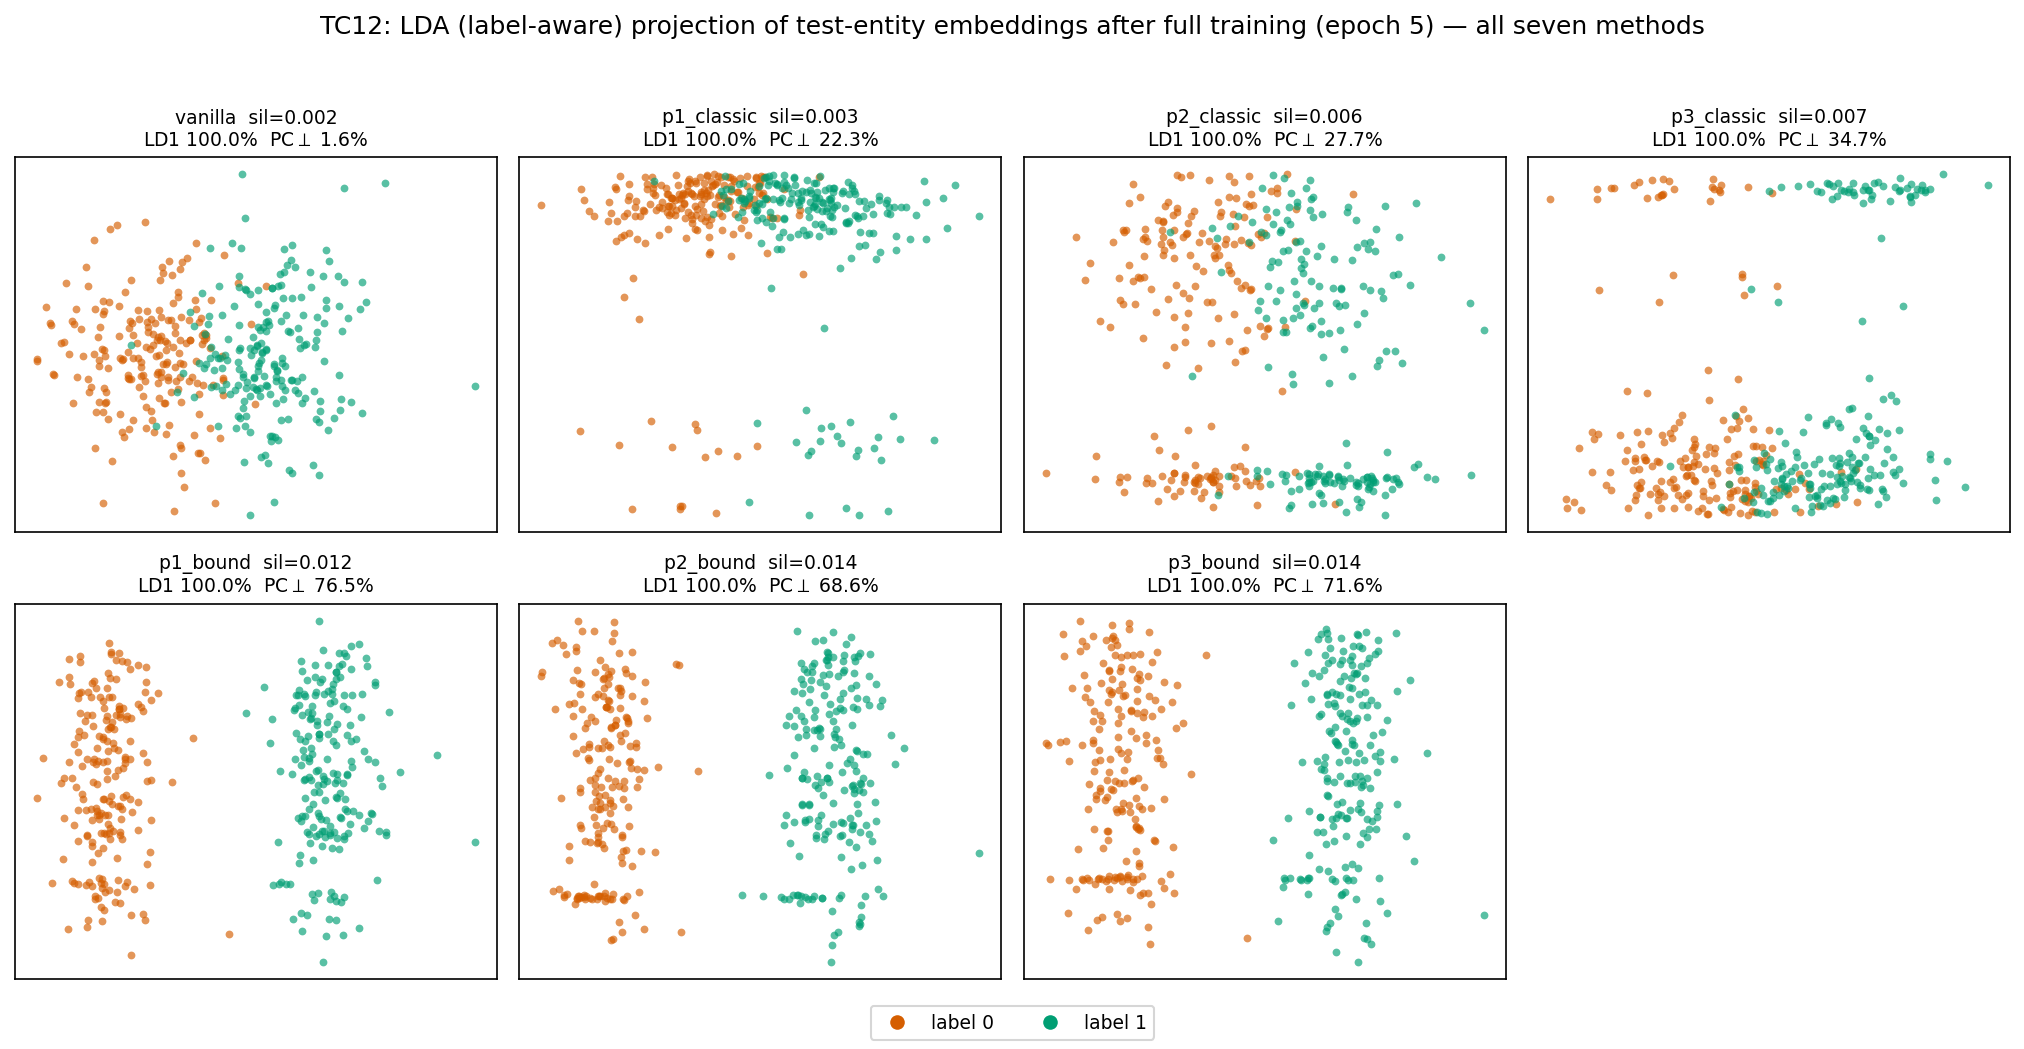
\includegraphics[width=\dimexpr\paperwidth-3cm\relax]{assets/lda/tc12_lda.png}}
  \end{longtable}
  \end{center}

\section{PCA Fine-Tune Drift for All Synthetic Test Cases}
\label{app:pca-drift-all}

Figure~\ref{fig:pca_drift_all_tcs} in Section~\ref{sec:results_drift} shows the
PCA fine-tune drift for the representative test case tc07. This appendix
reproduces the same diagnostic for the remaining fourteen DLCC synthetic test
cases (tc01--tc06 and tc08--tc15), confirming that the pattern holds across the
whole benchmark and not only on the showcase case.

In each panel the held-out test entities of one variant are projected onto a PCA
basis fitted jointly on their epoch-0 and epoch-5 vectors: faint markers are the
entities at initialization, bold markers the same entities after fine-tuning,
and arrows connect the two (marker colour is the binary DLCC label). The panel
title reports held-out accuracy at initialization $\rightarrow$ after
fine-tuning and the mean epoch-0/epoch-5 cosine; this cosine, not the visual
class overlap, is the reliable measure of movement, since PCA selects
high-variance rather than label-discriminative directions. The contrast is
consistent with the main text: \texttt{vanilla} and the classic variants drift
far (long arrows, low cosine), while the concept-bound variants under the
protected learning rate barely move. The per-panel layout is given in the figure
caption.

\begin{center}
  \captionsetup{type=figure}
  \captionof{figure}{PCA fine-tune drift (epoch 0 $\rightarrow$ epoch 5) of the
  held-out test entities for the remaining DLCC synthetic test cases
  (tc01--tc06 and tc08--tc15); tc07 is shown in
  Figure~\ref{fig:pca_drift_all_tcs}. Each panel shares a PCA basis fitted on the
  union of the epoch-0 (faint) and epoch-5 (bold) vectors; arrows connect each
  entity's initialization to its fine-tuned position. Top-left: the
  \texttt{vanilla} baseline (no protograph initialization, LR $0.025$); rest of
  the top row: classic initializations (P1/P2/P3) at LR $0.025$;
  bottom row: concept-bound initializations (P1/P2/P3) at the protected LR
  $0.0025$. Panel titles report accuracy at initialization $\rightarrow$ after
  fine-tuning and the mean epoch-0/epoch-5 cosine.}
  \label{fig:pca_drift_appendix}

  \begin{longtable}{c}
  \makebox[\linewidth][c]{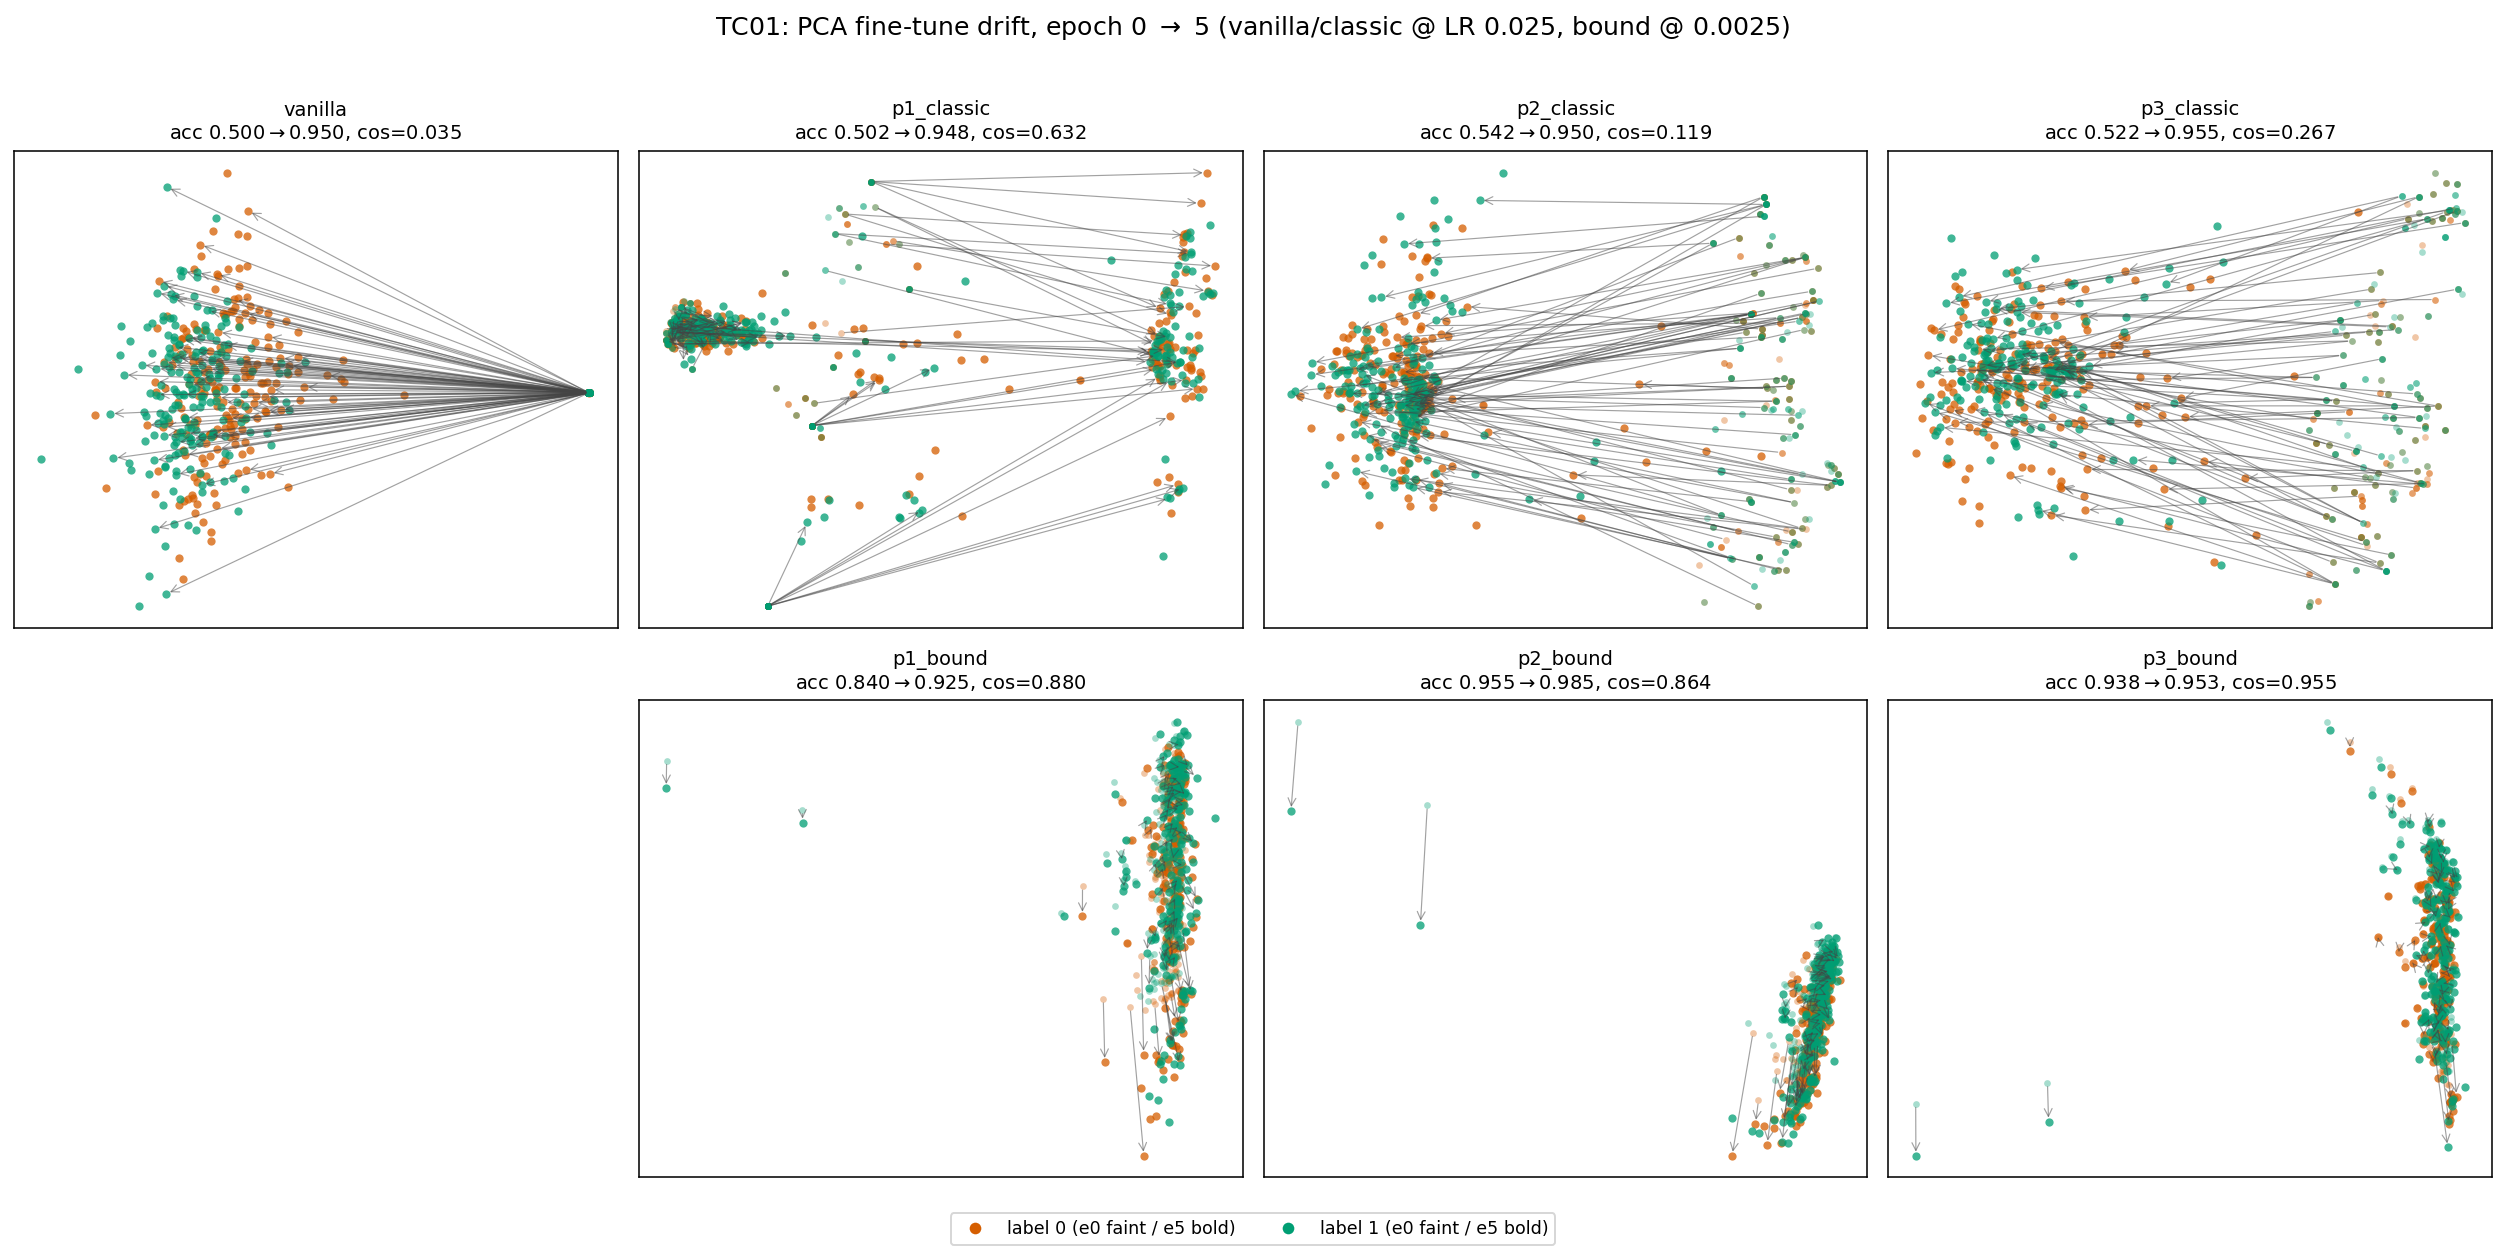
\includegraphics[width=\dimexpr\paperwidth-3cm\relax]{assets/pca_drift/tc01_pca_drift.png}} \\[1.0em]

  \makebox[\linewidth][c]{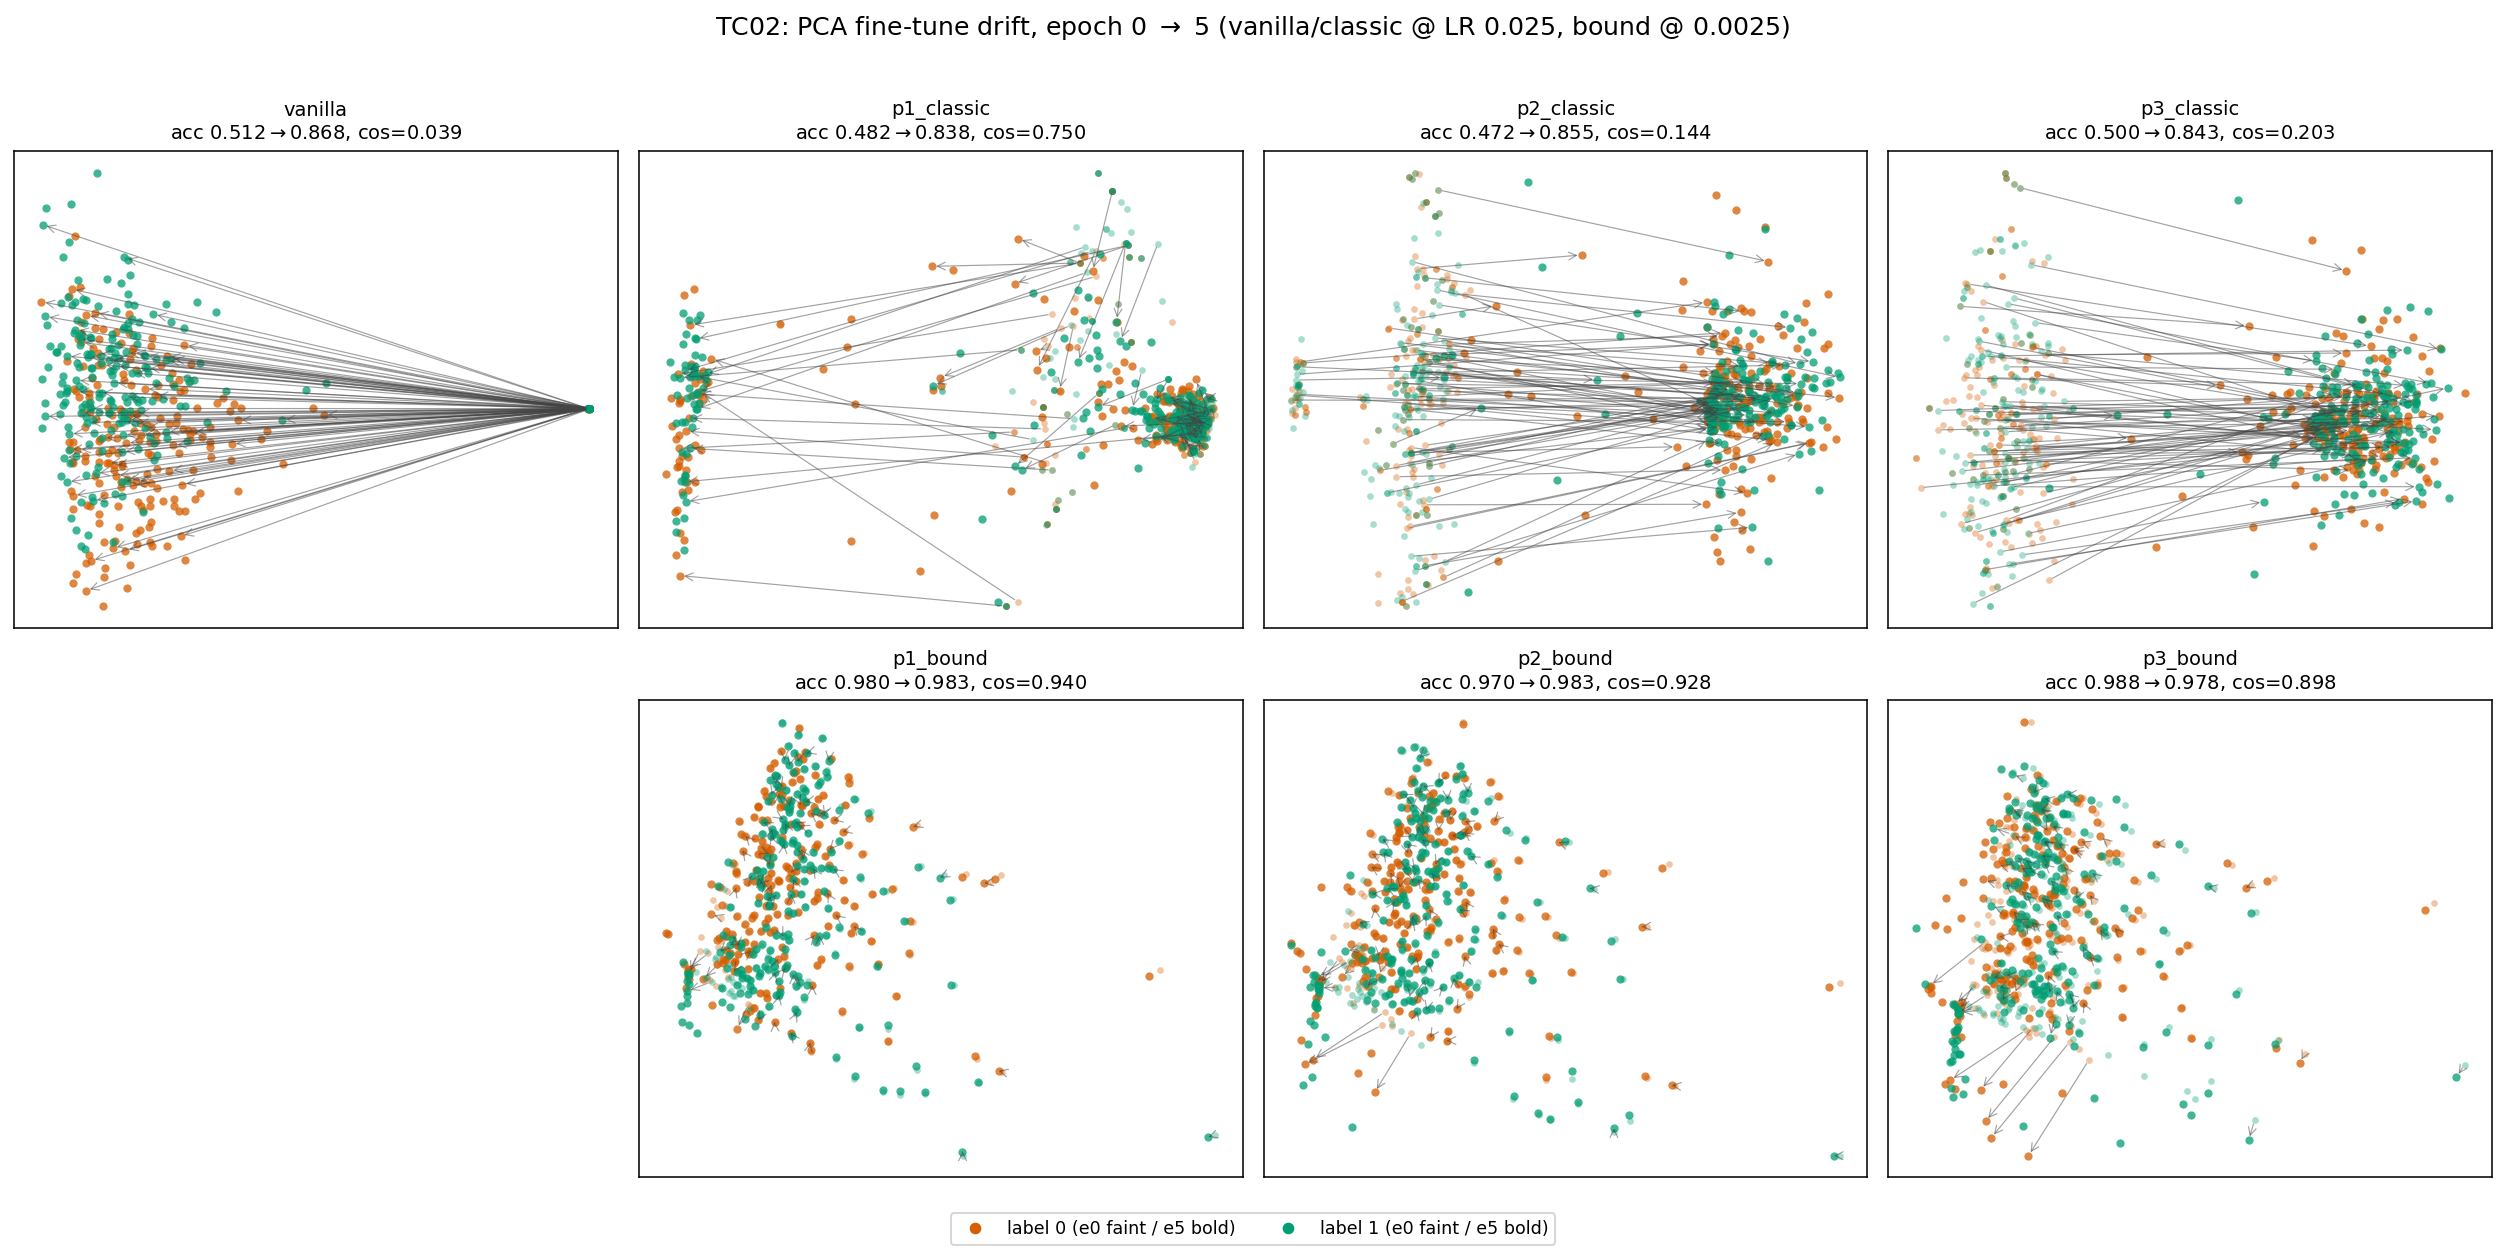
\includegraphics[width=\dimexpr\paperwidth-3cm\relax]{assets/pca_drift/tc02_pca_drift.png}} \\[1.0em]

  \makebox[\linewidth][c]{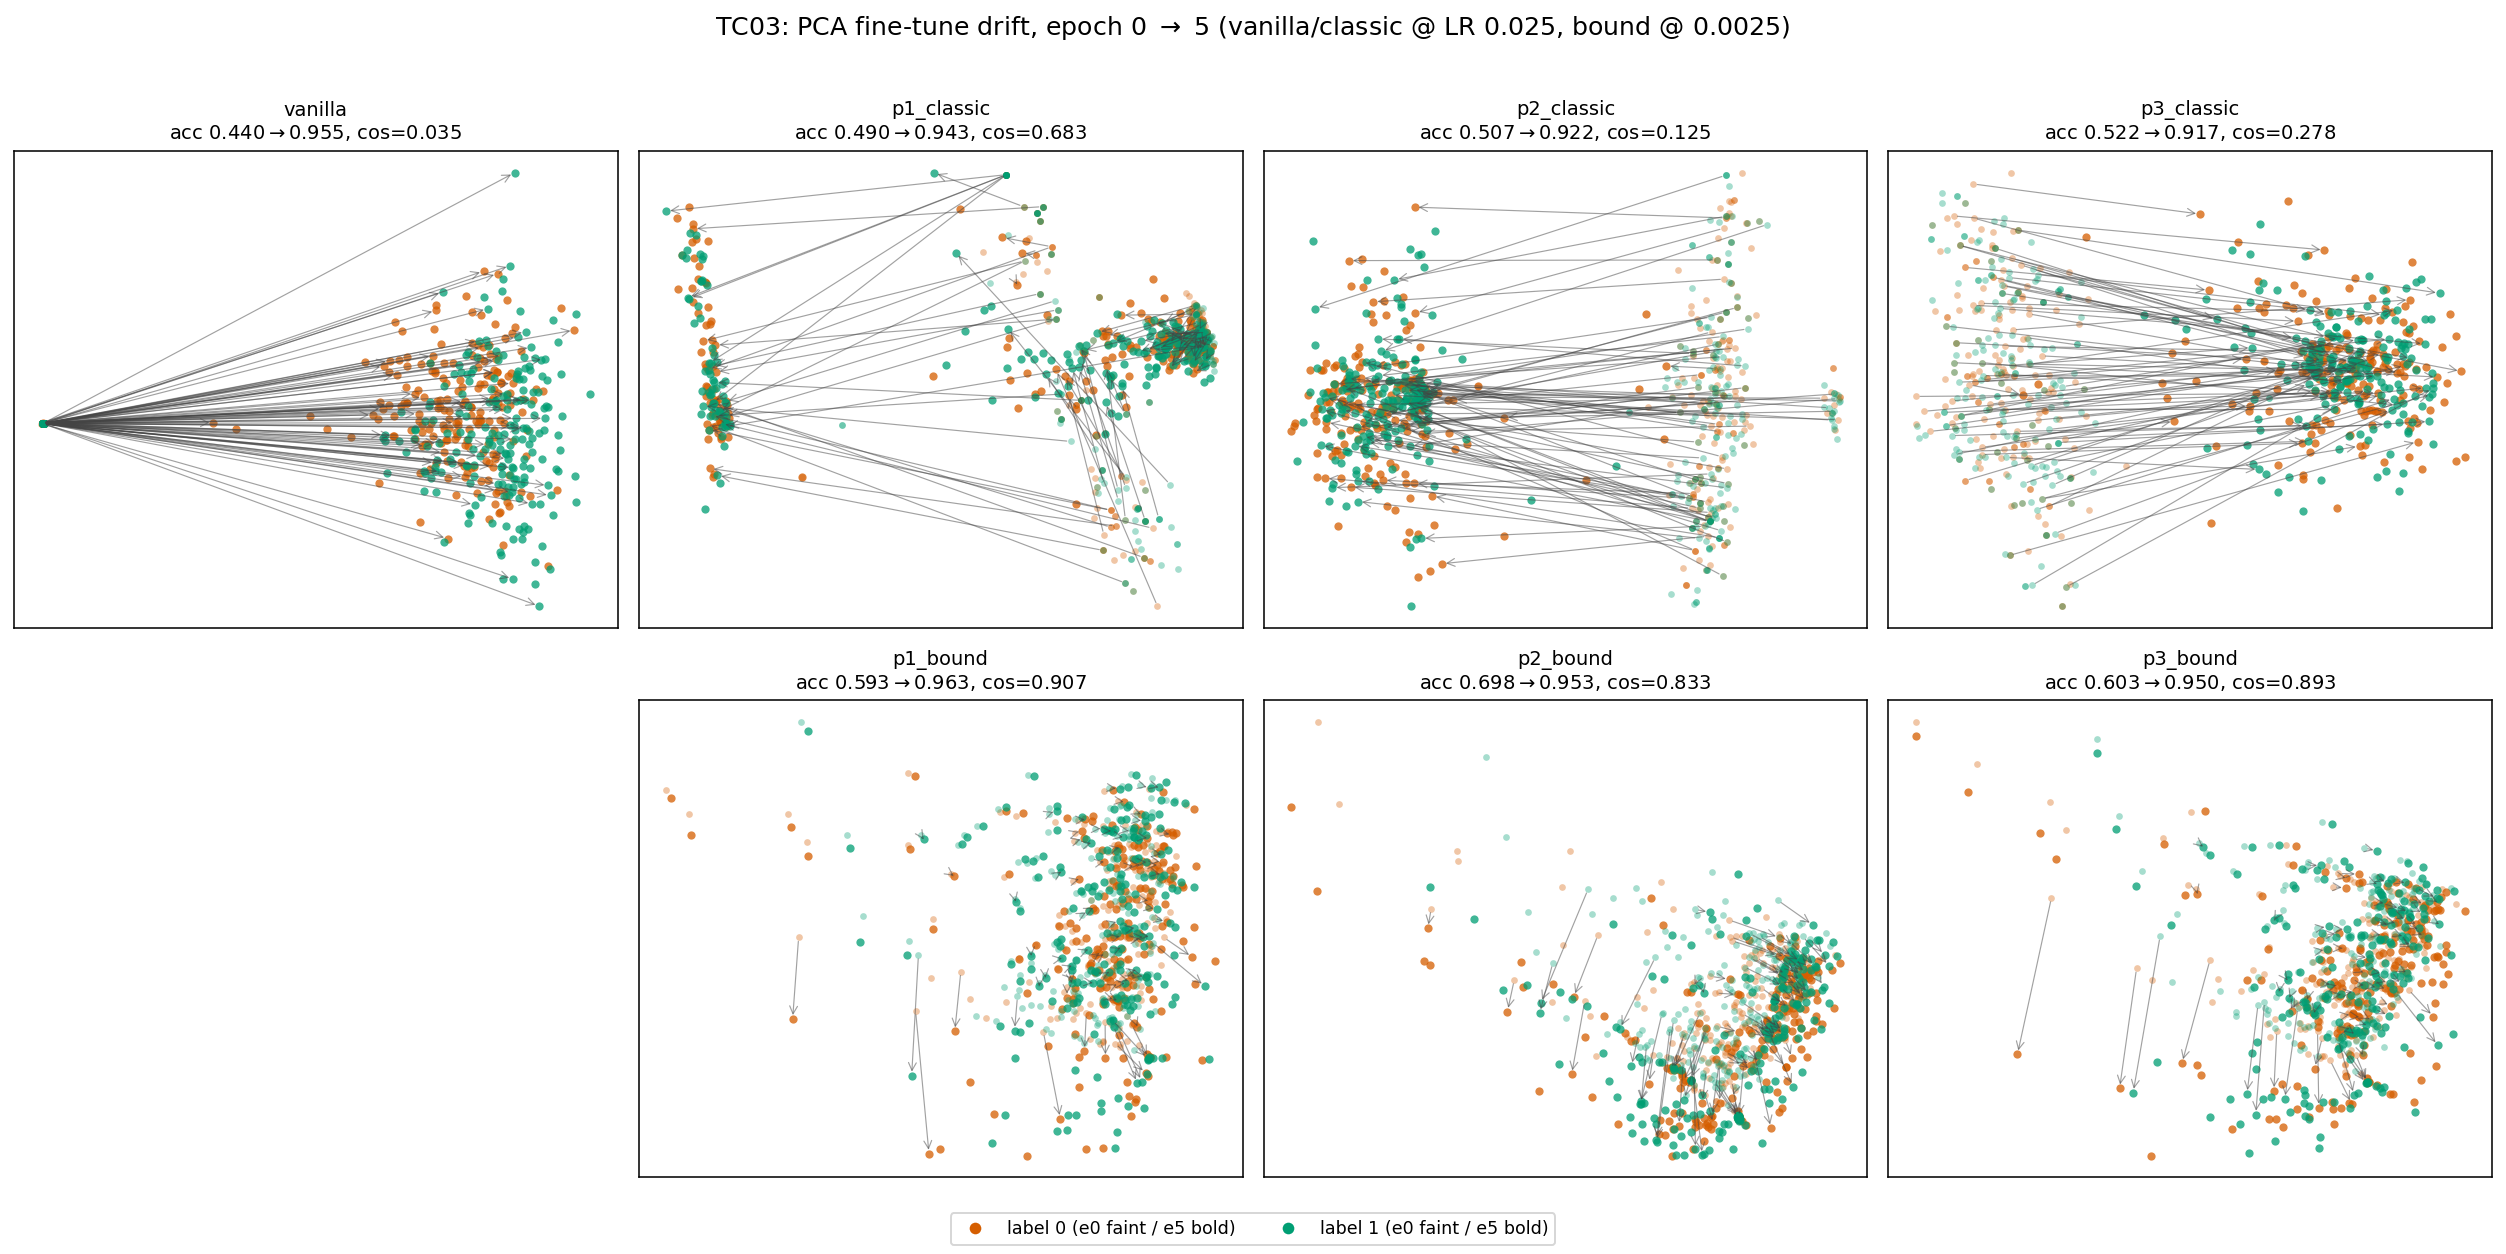
\includegraphics[width=\dimexpr\paperwidth-3cm\relax]{assets/pca_drift/tc03_pca_drift.png}} \\[1.0em]

  \makebox[\linewidth][c]{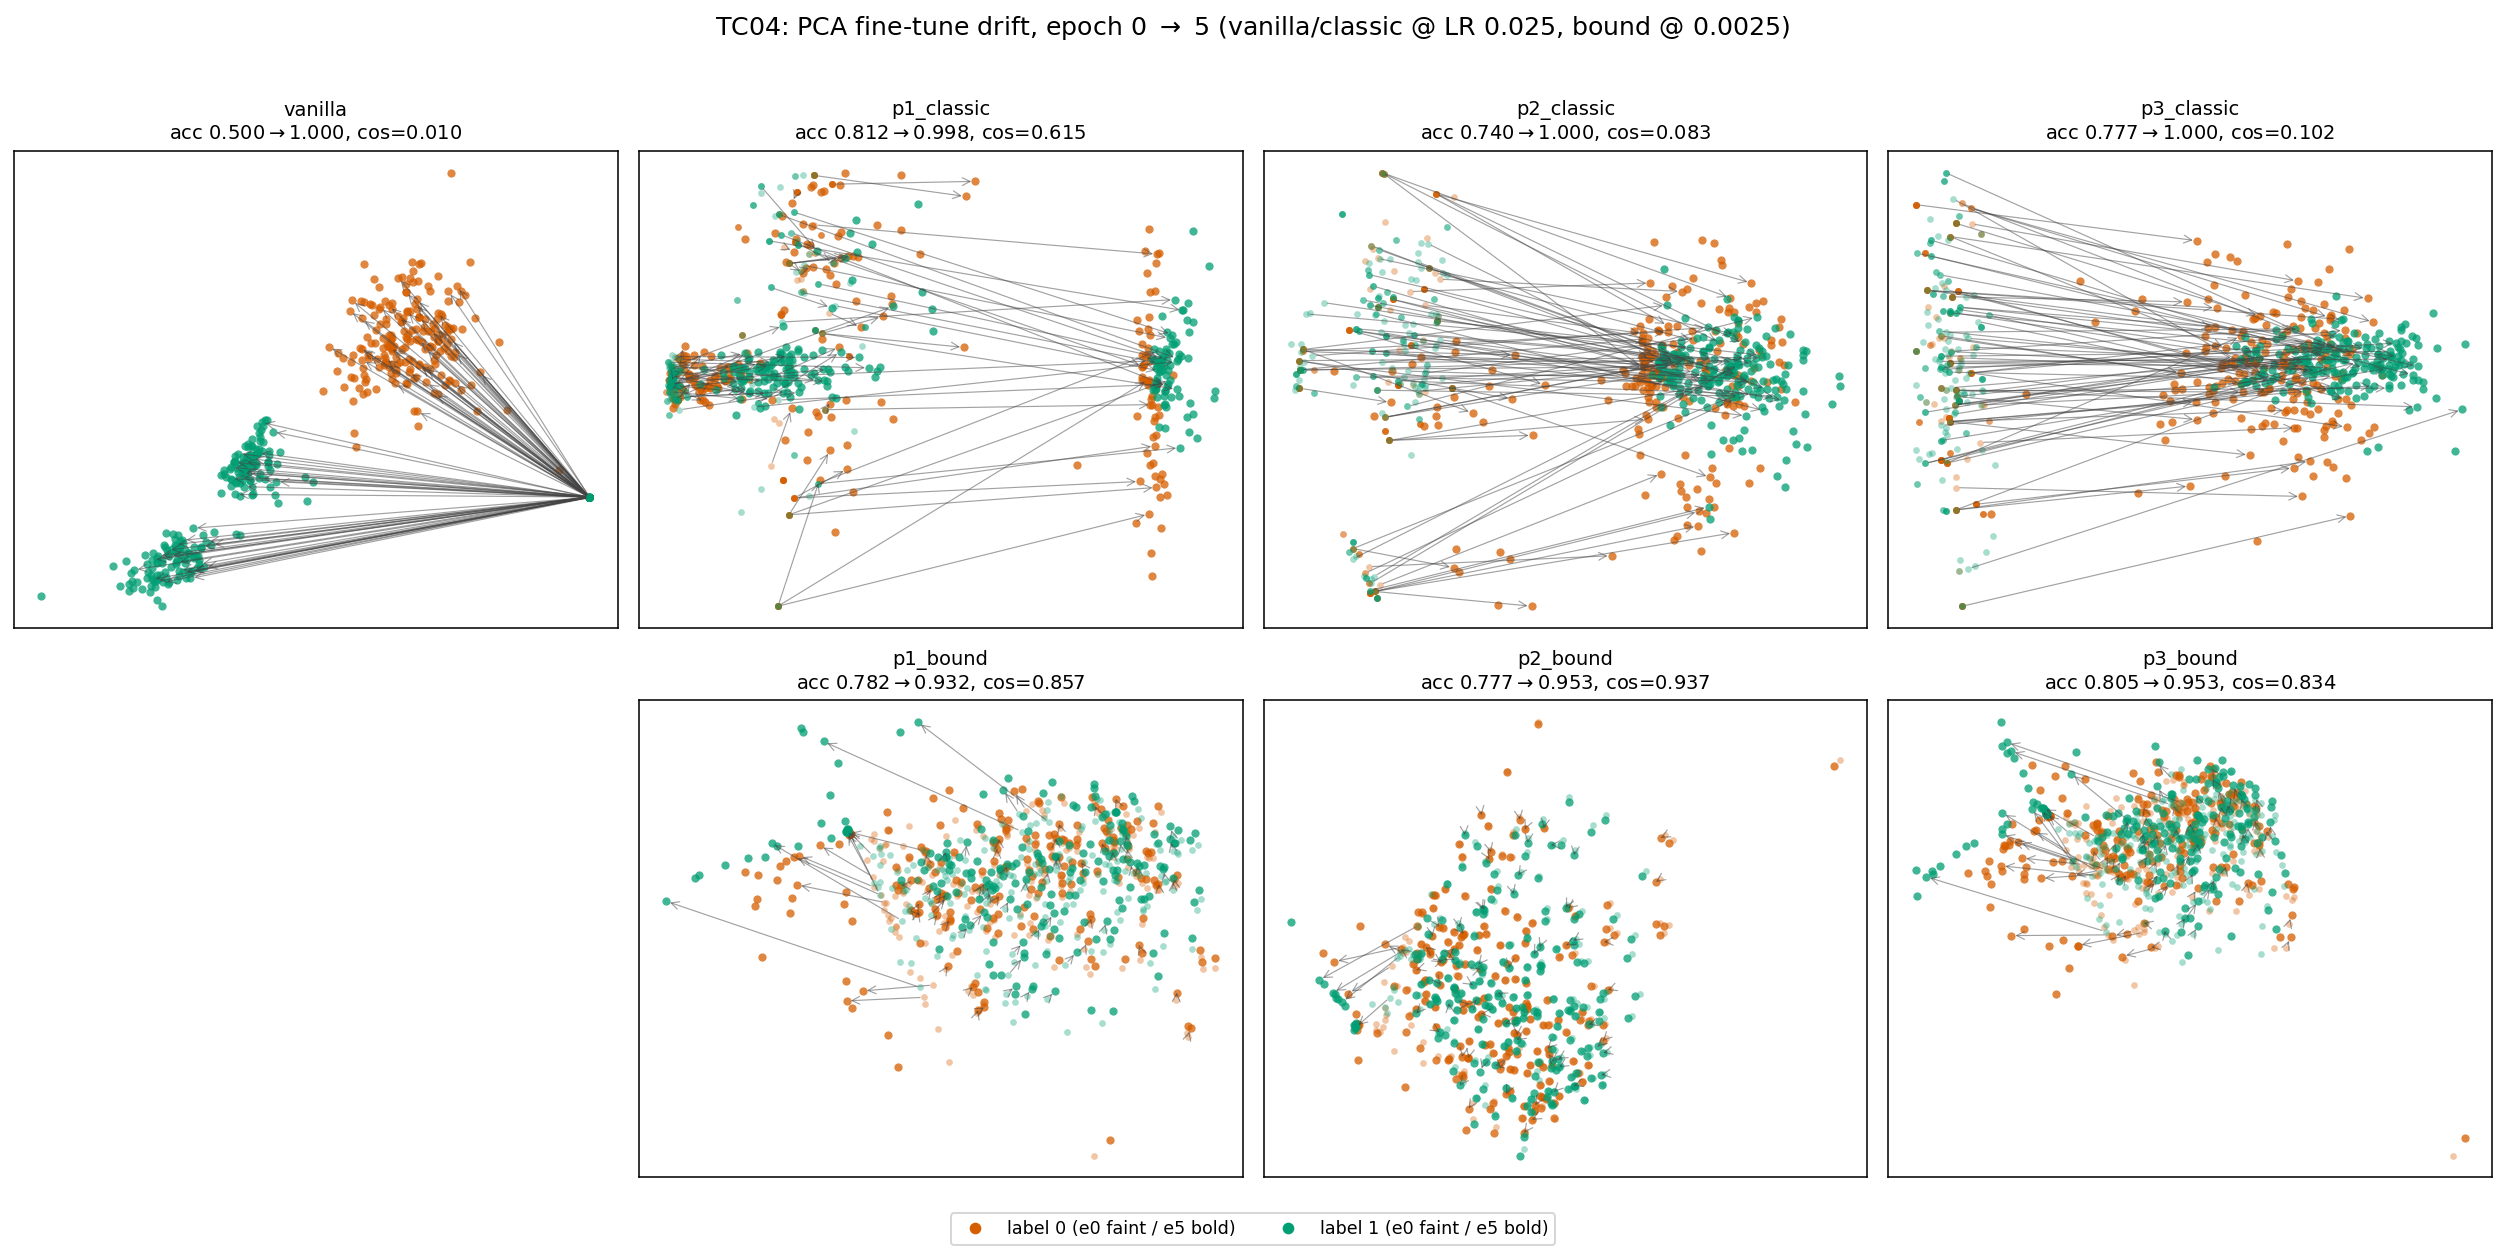
\includegraphics[width=\dimexpr\paperwidth-3cm\relax]{assets/pca_drift/tc04_pca_drift.png}} \\[1.0em]

  \makebox[\linewidth][c]{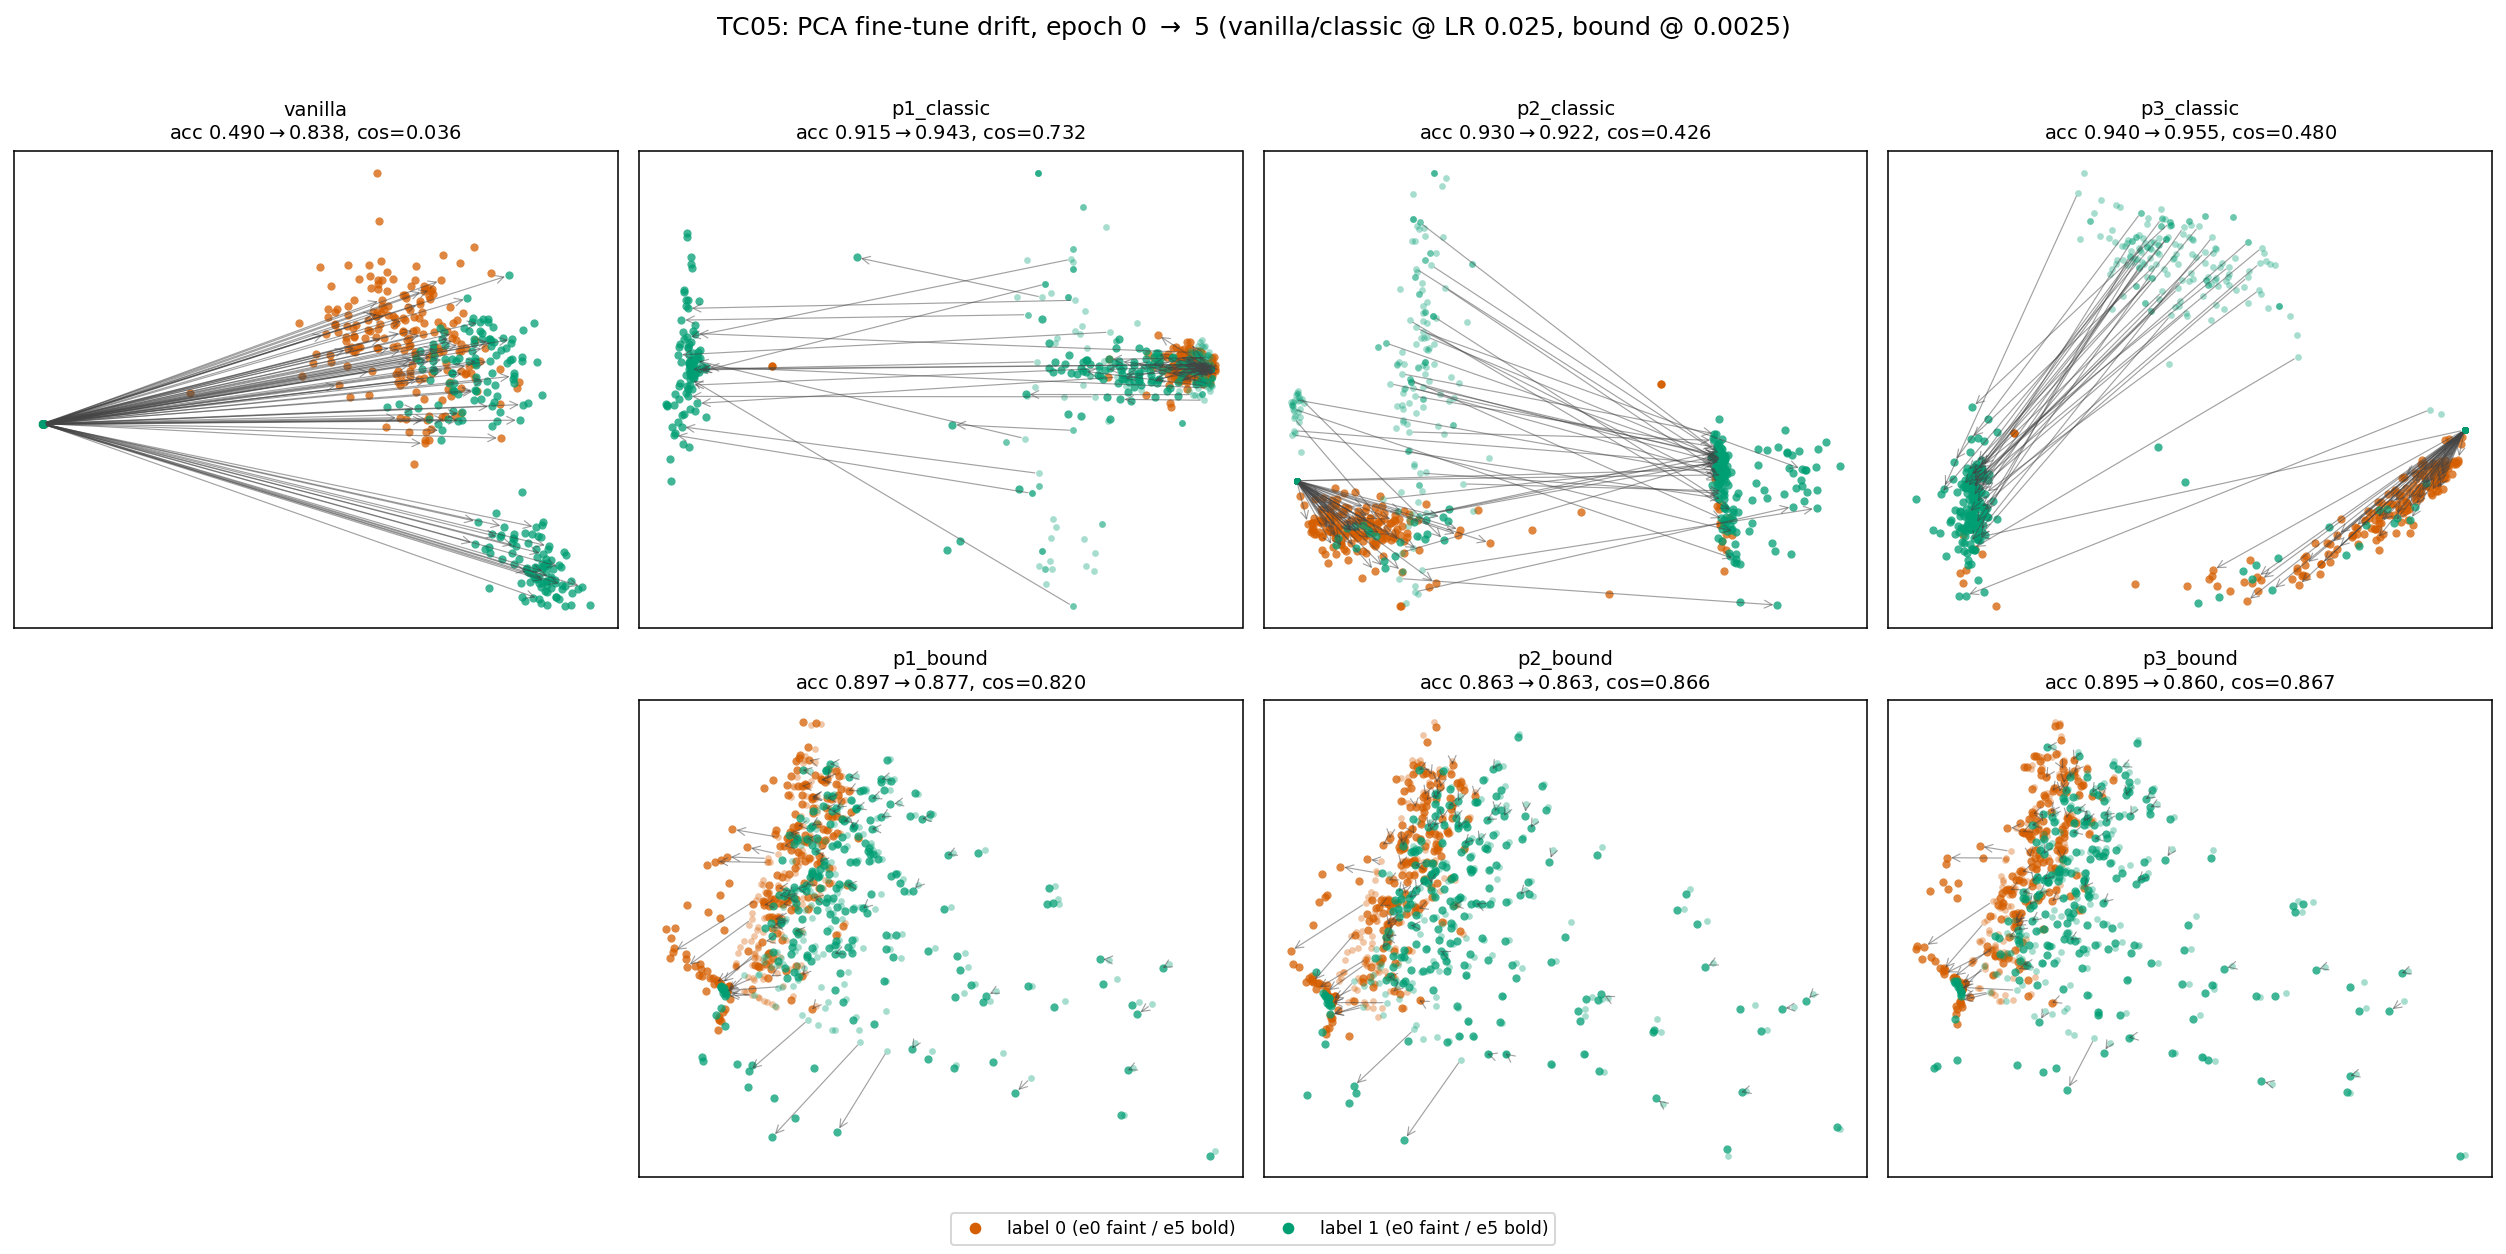
\includegraphics[width=\dimexpr\paperwidth-3cm\relax]{assets/pca_drift/tc05_pca_drift.png}} \\[1.0em]

  \makebox[\linewidth][c]{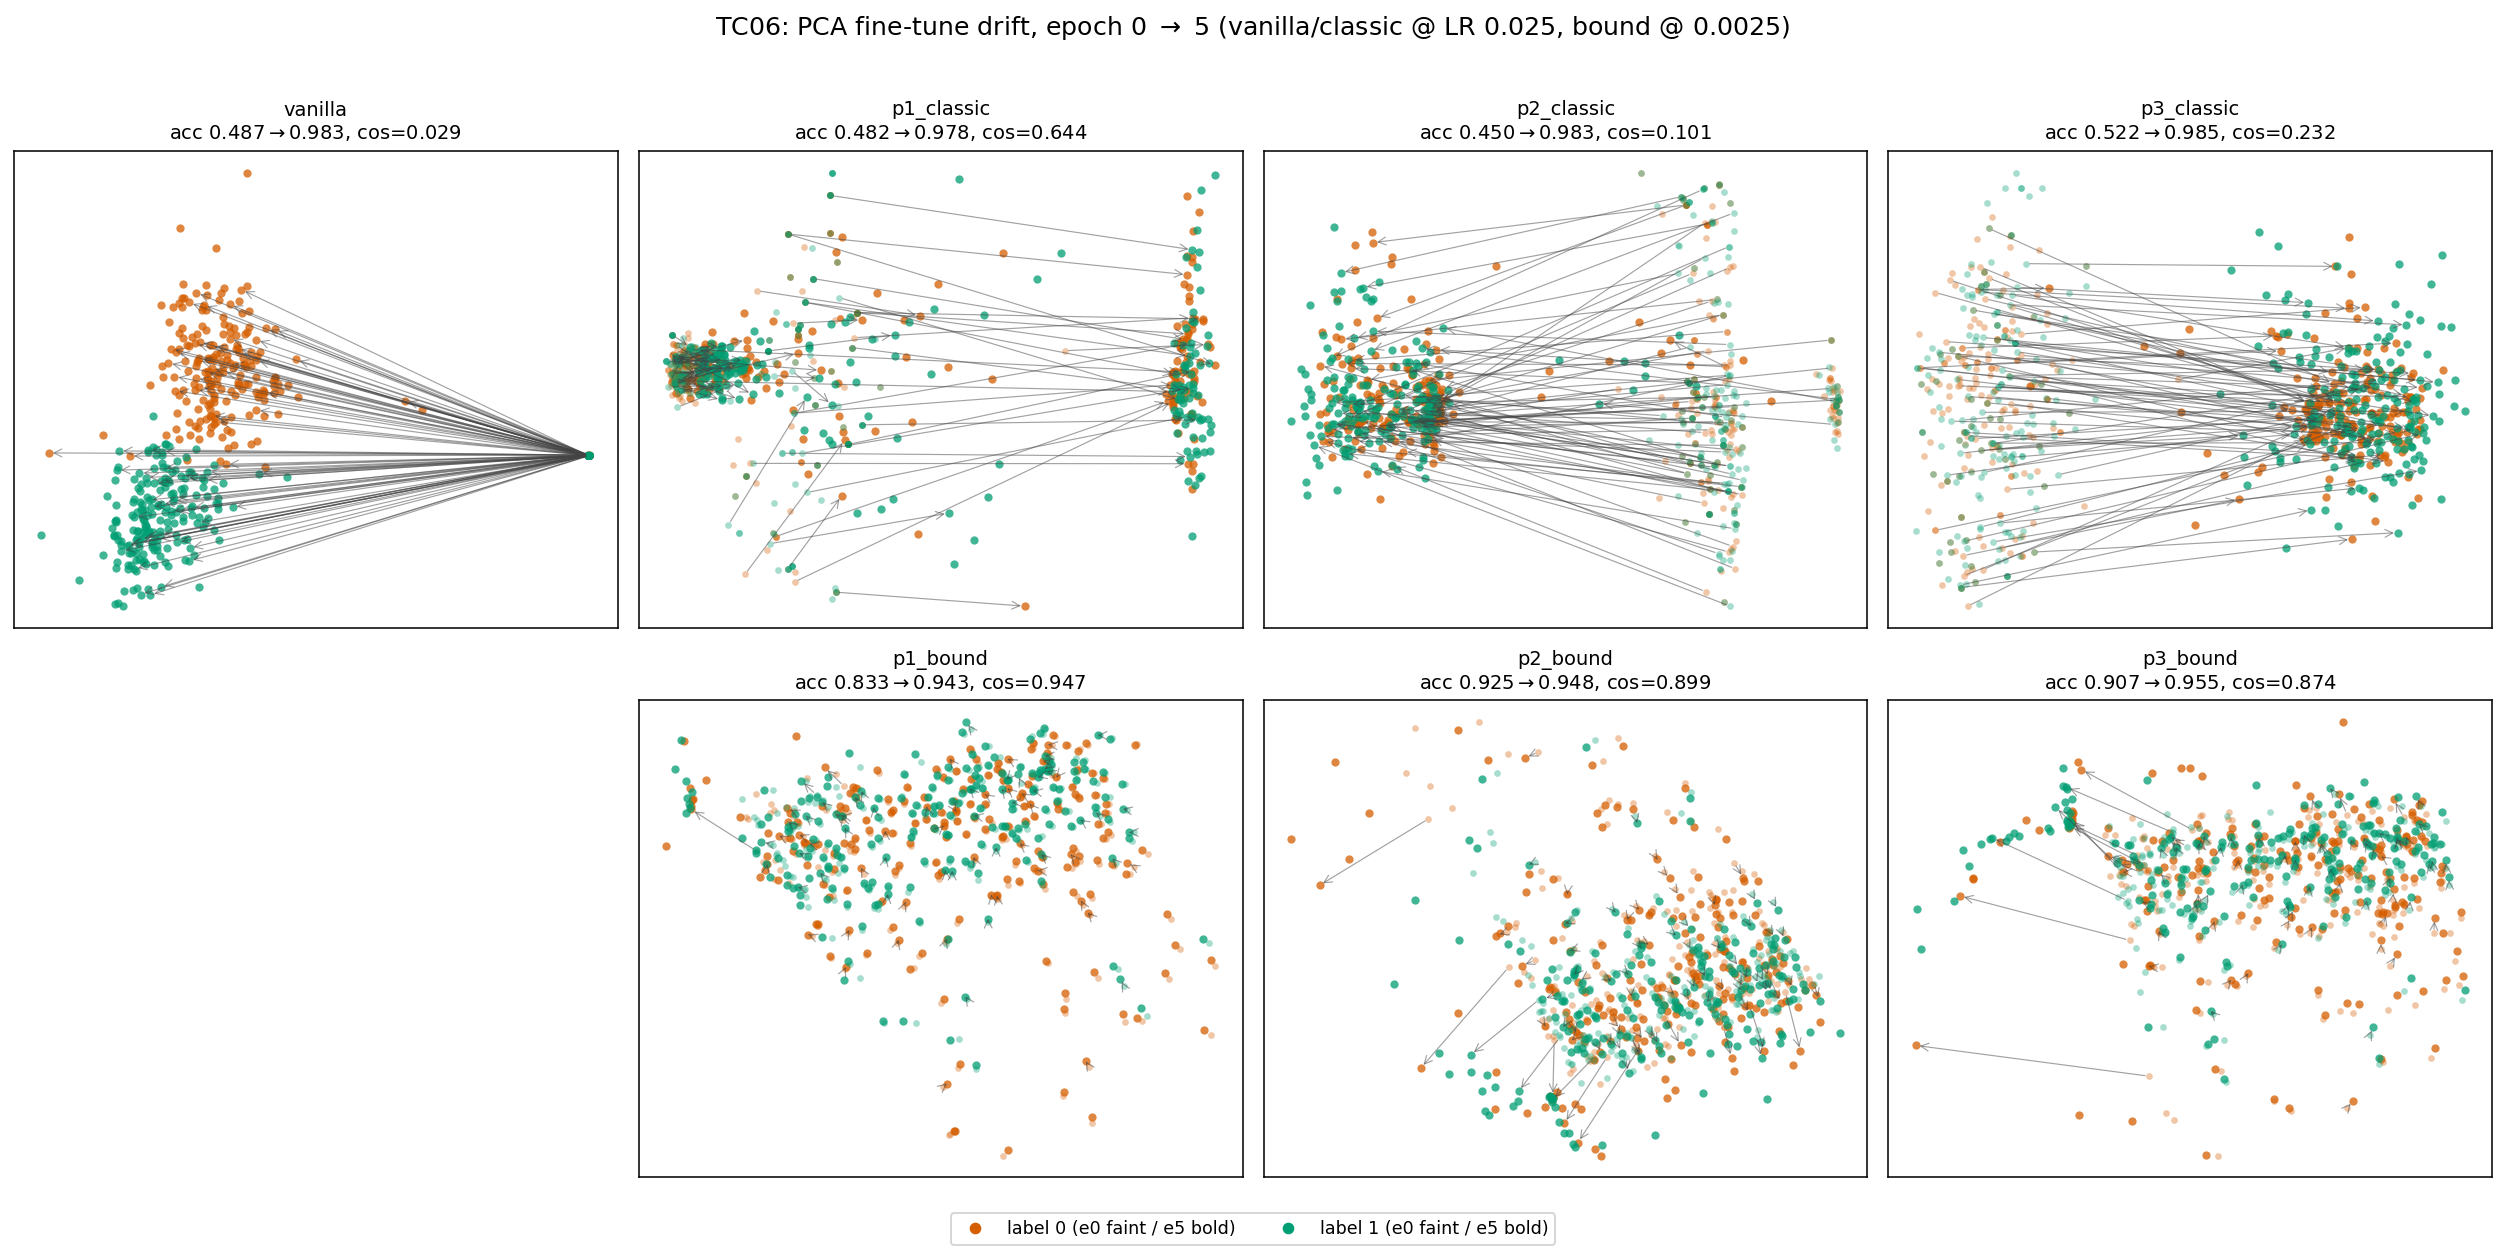
\includegraphics[width=\dimexpr\paperwidth-3cm\relax]{assets/pca_drift/tc06_pca_drift.png}} \\[1.0em]

  \makebox[\linewidth][c]{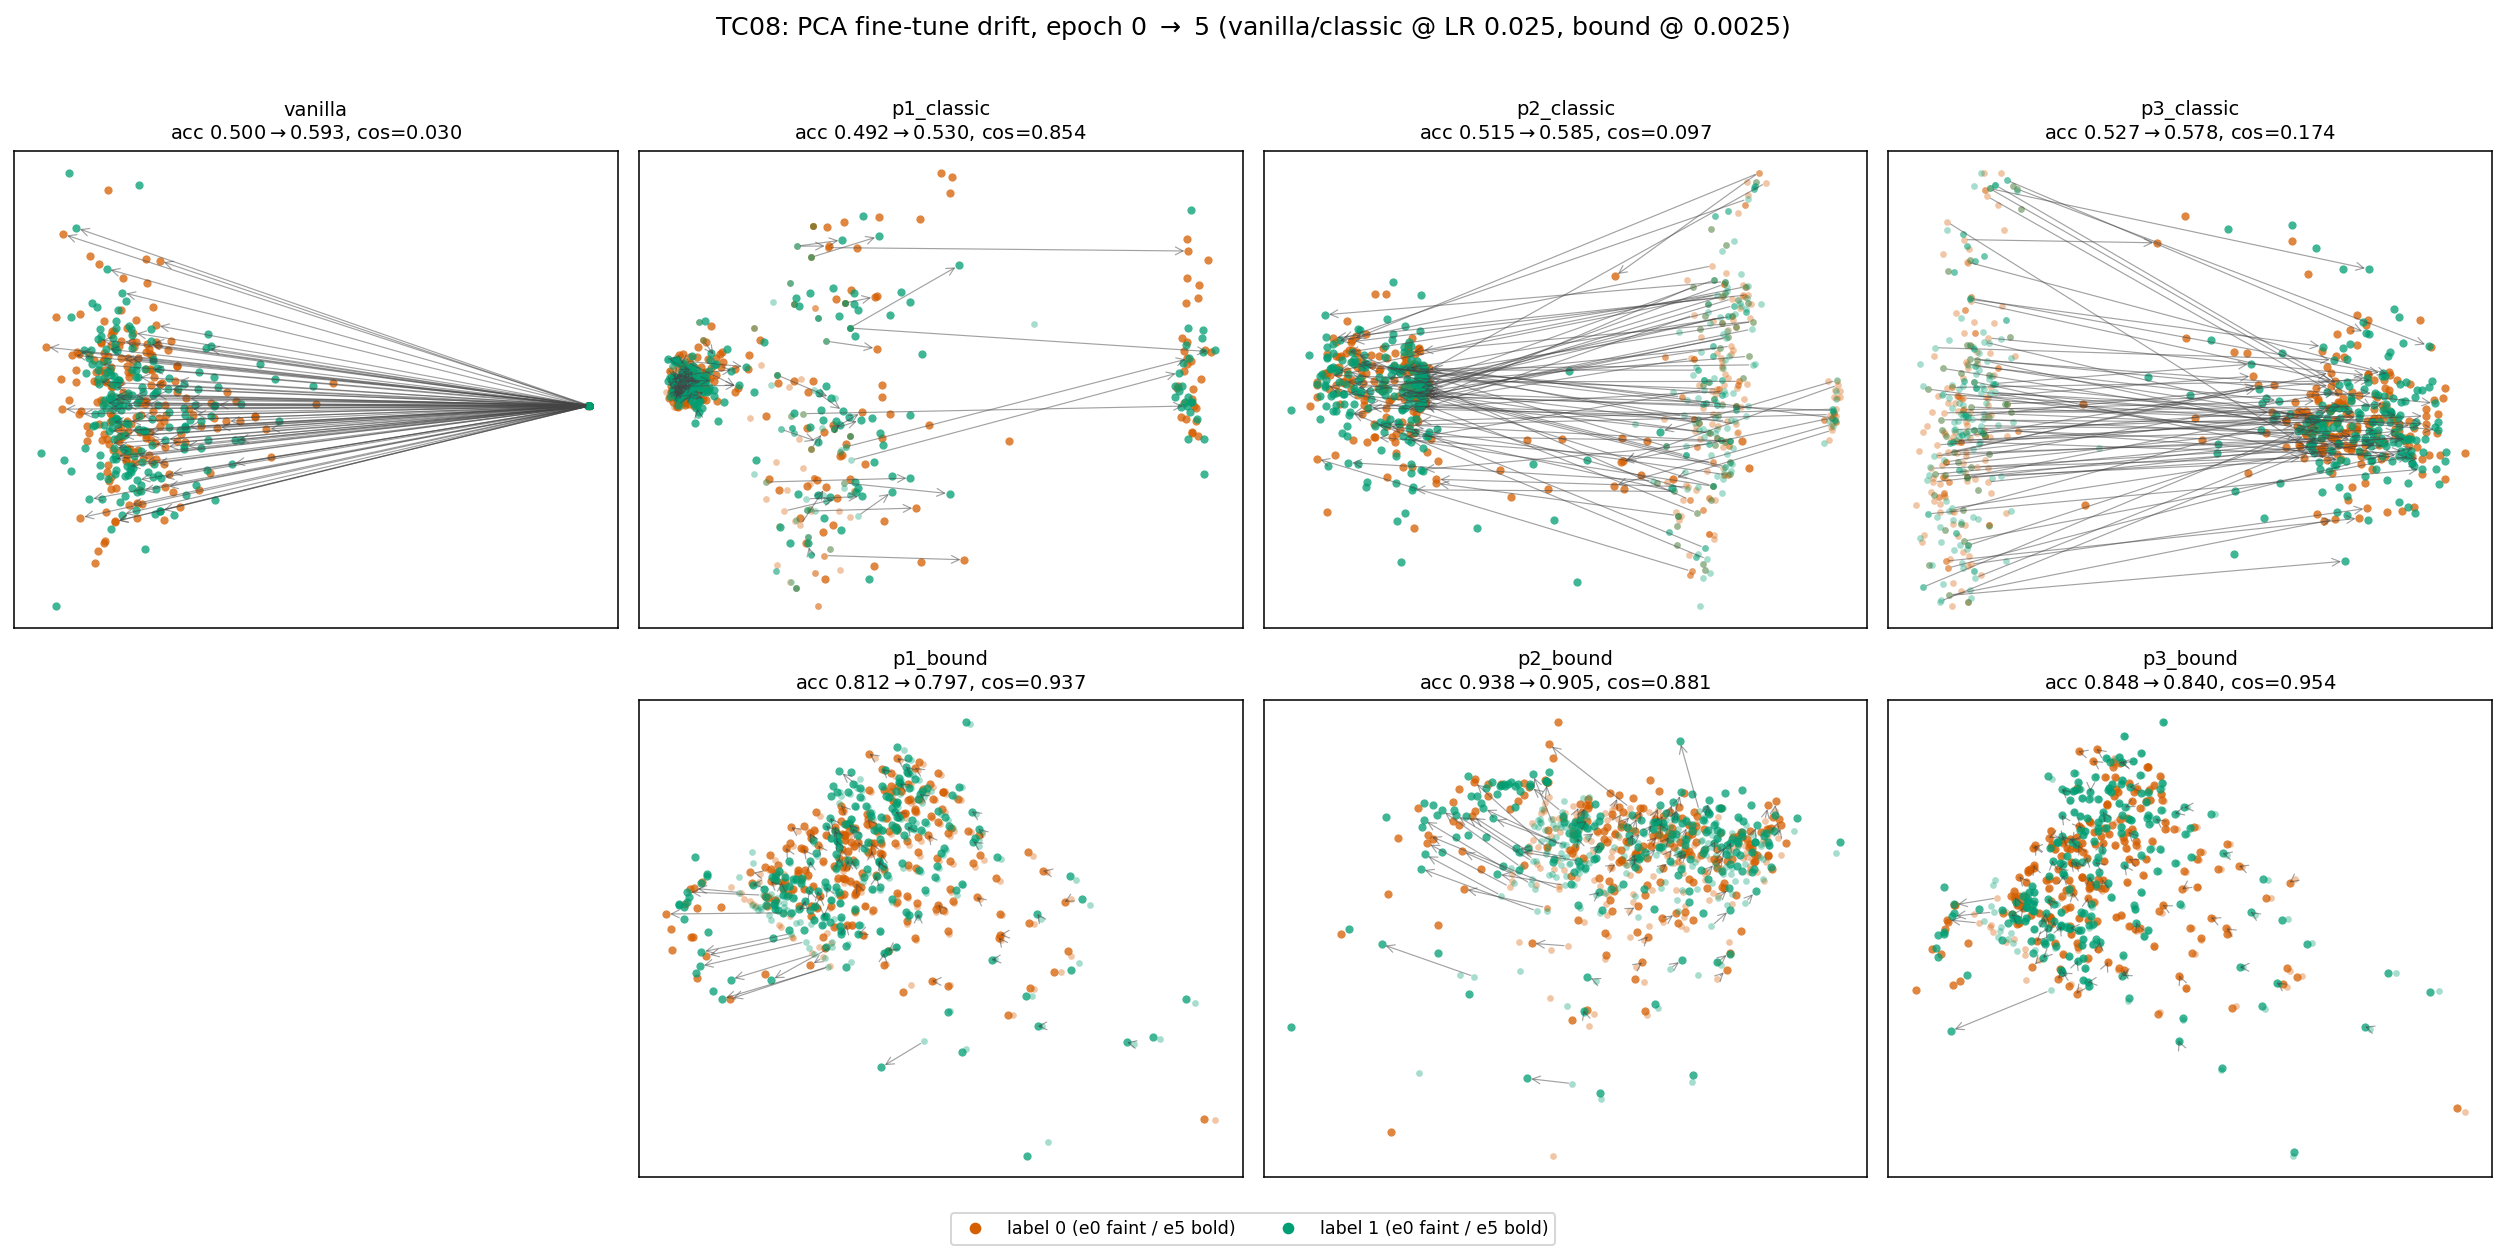
\includegraphics[width=\dimexpr\paperwidth-3cm\relax]{assets/pca_drift/tc08_pca_drift.png}} \\[1.0em]

  \makebox[\linewidth][c]{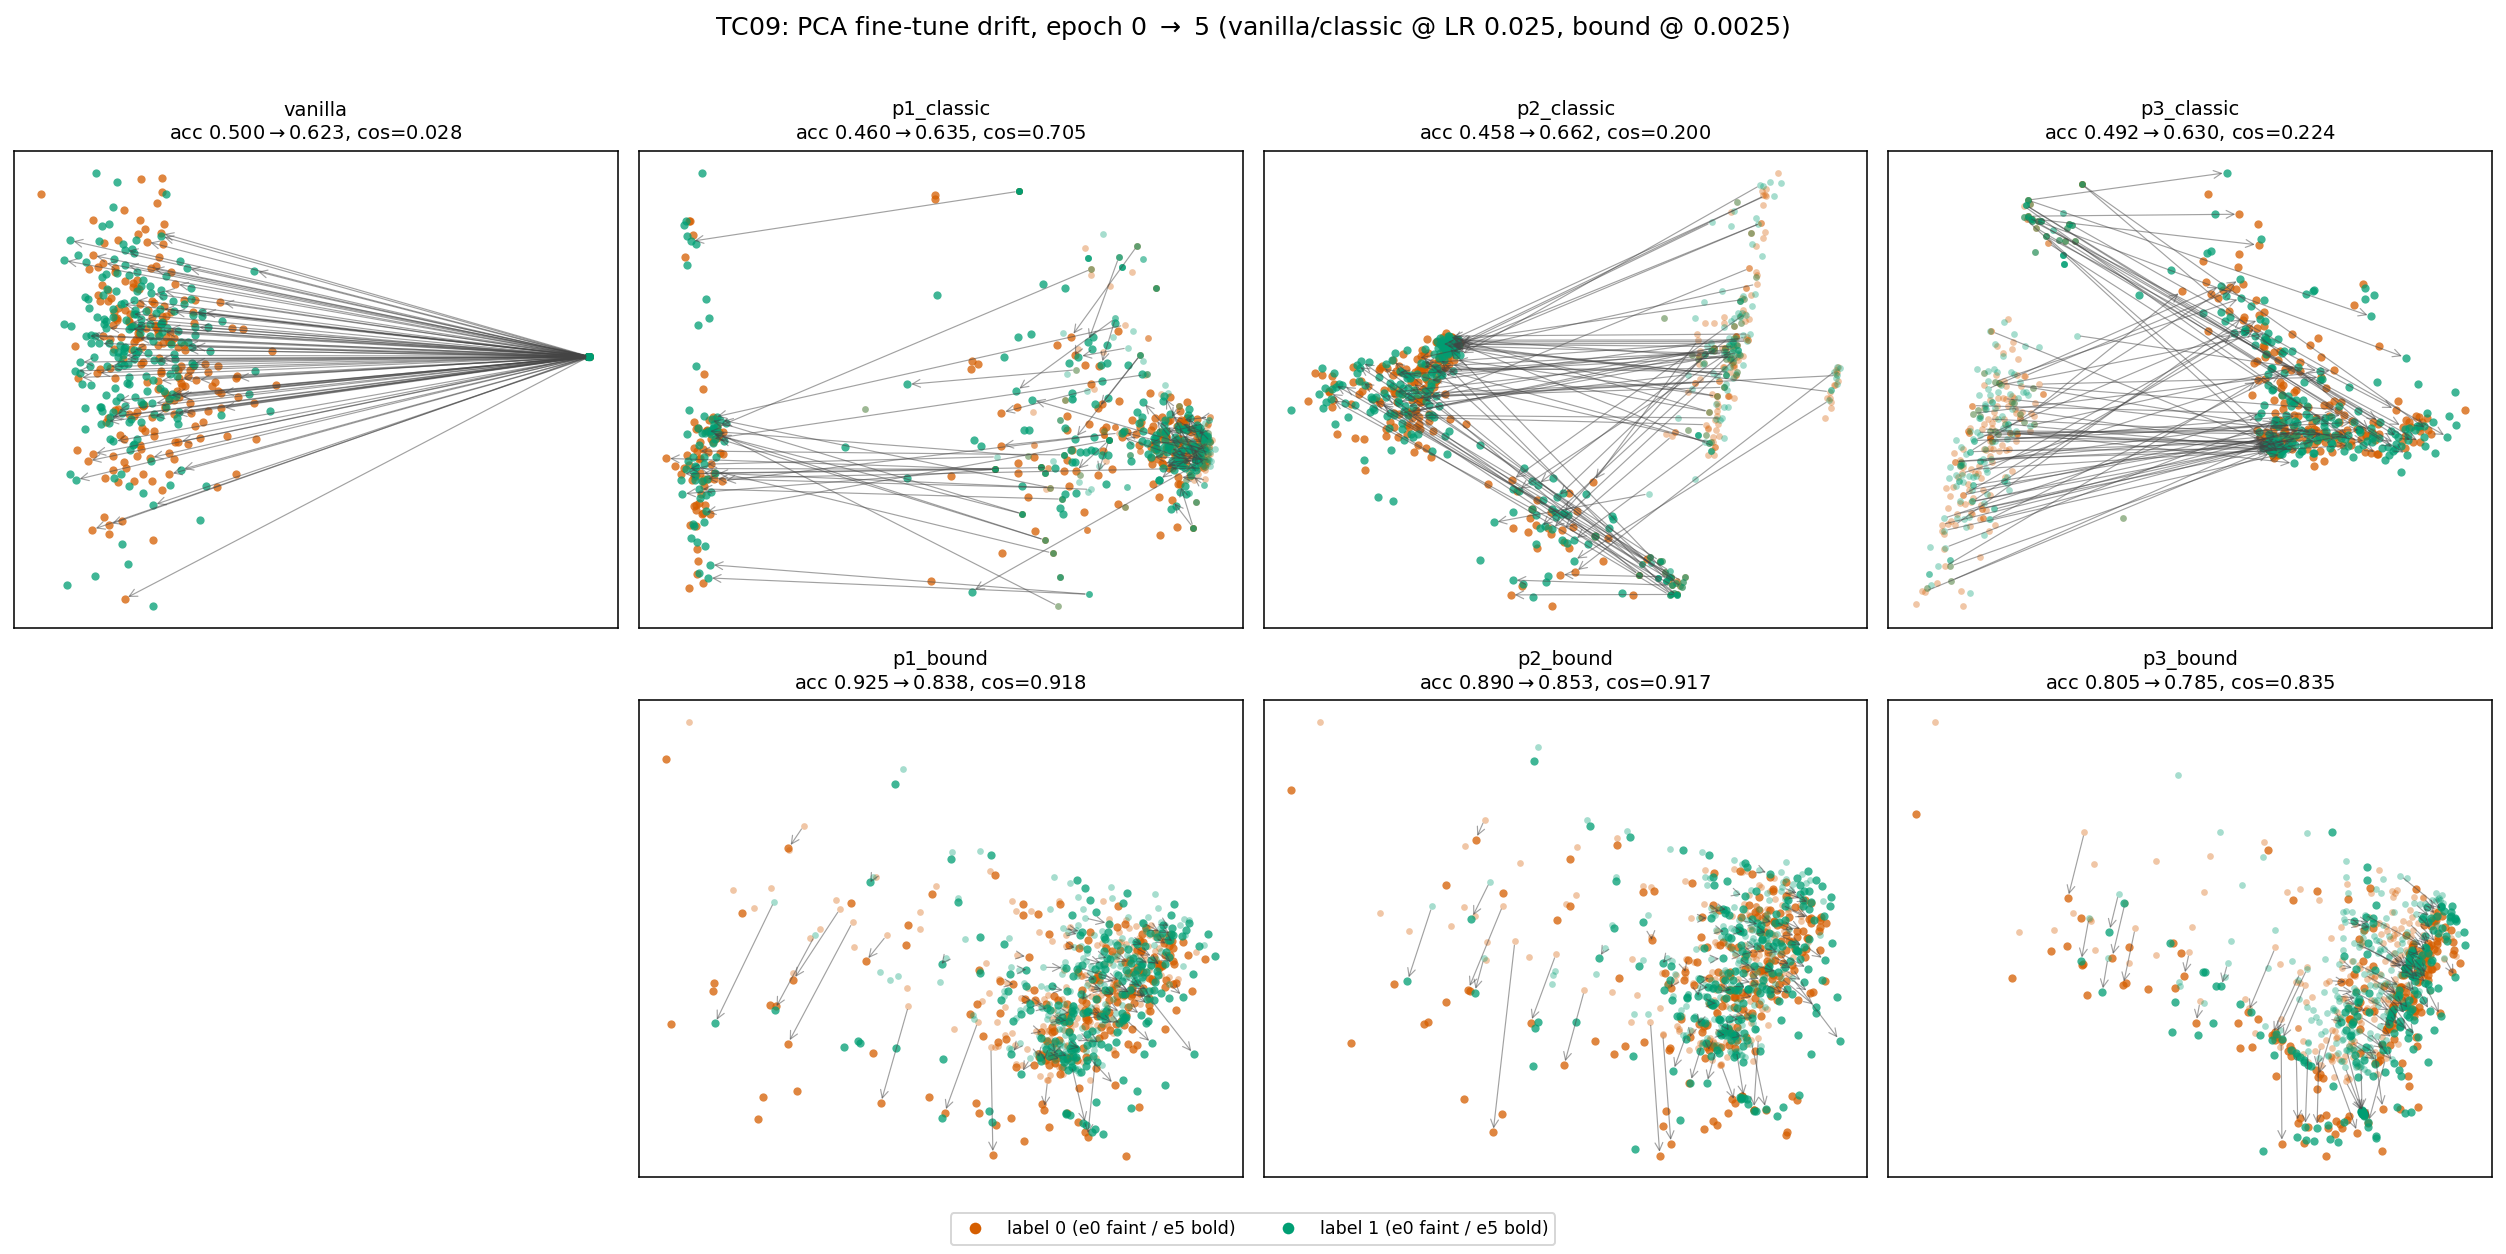
\includegraphics[width=\dimexpr\paperwidth-3cm\relax]{assets/pca_drift/tc09_pca_drift.png}} \\[1.0em]

  \makebox[\linewidth][c]{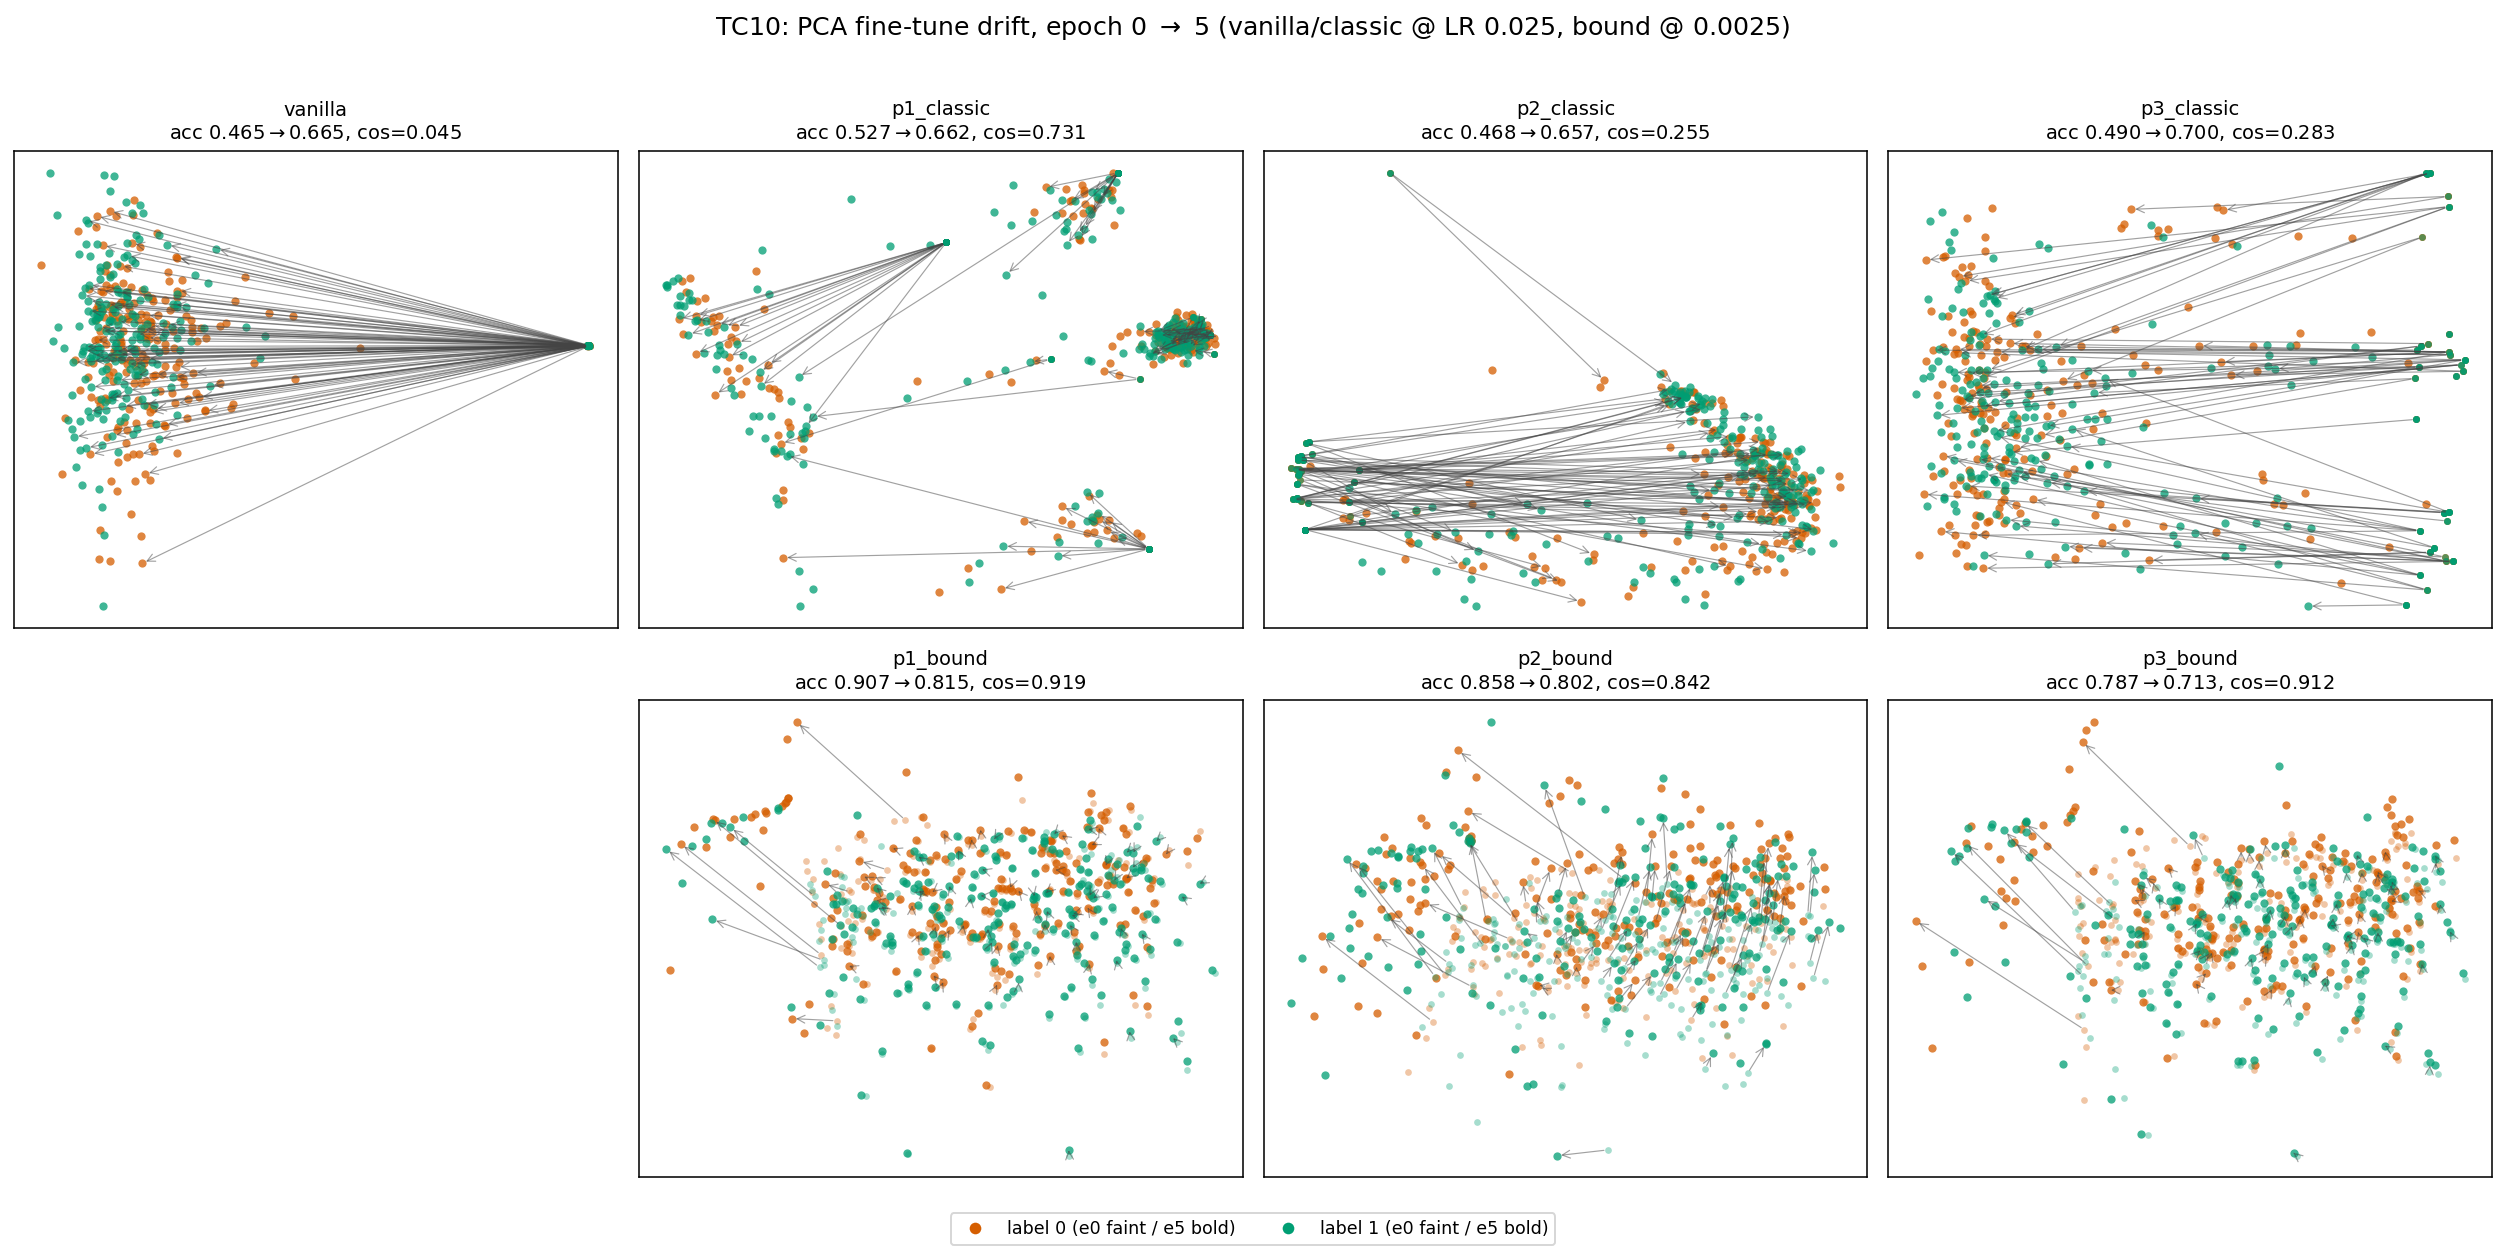
\includegraphics[width=\dimexpr\paperwidth-3cm\relax]{assets/pca_drift/tc10_pca_drift.png}} \\[1.0em]

  \makebox[\linewidth][c]{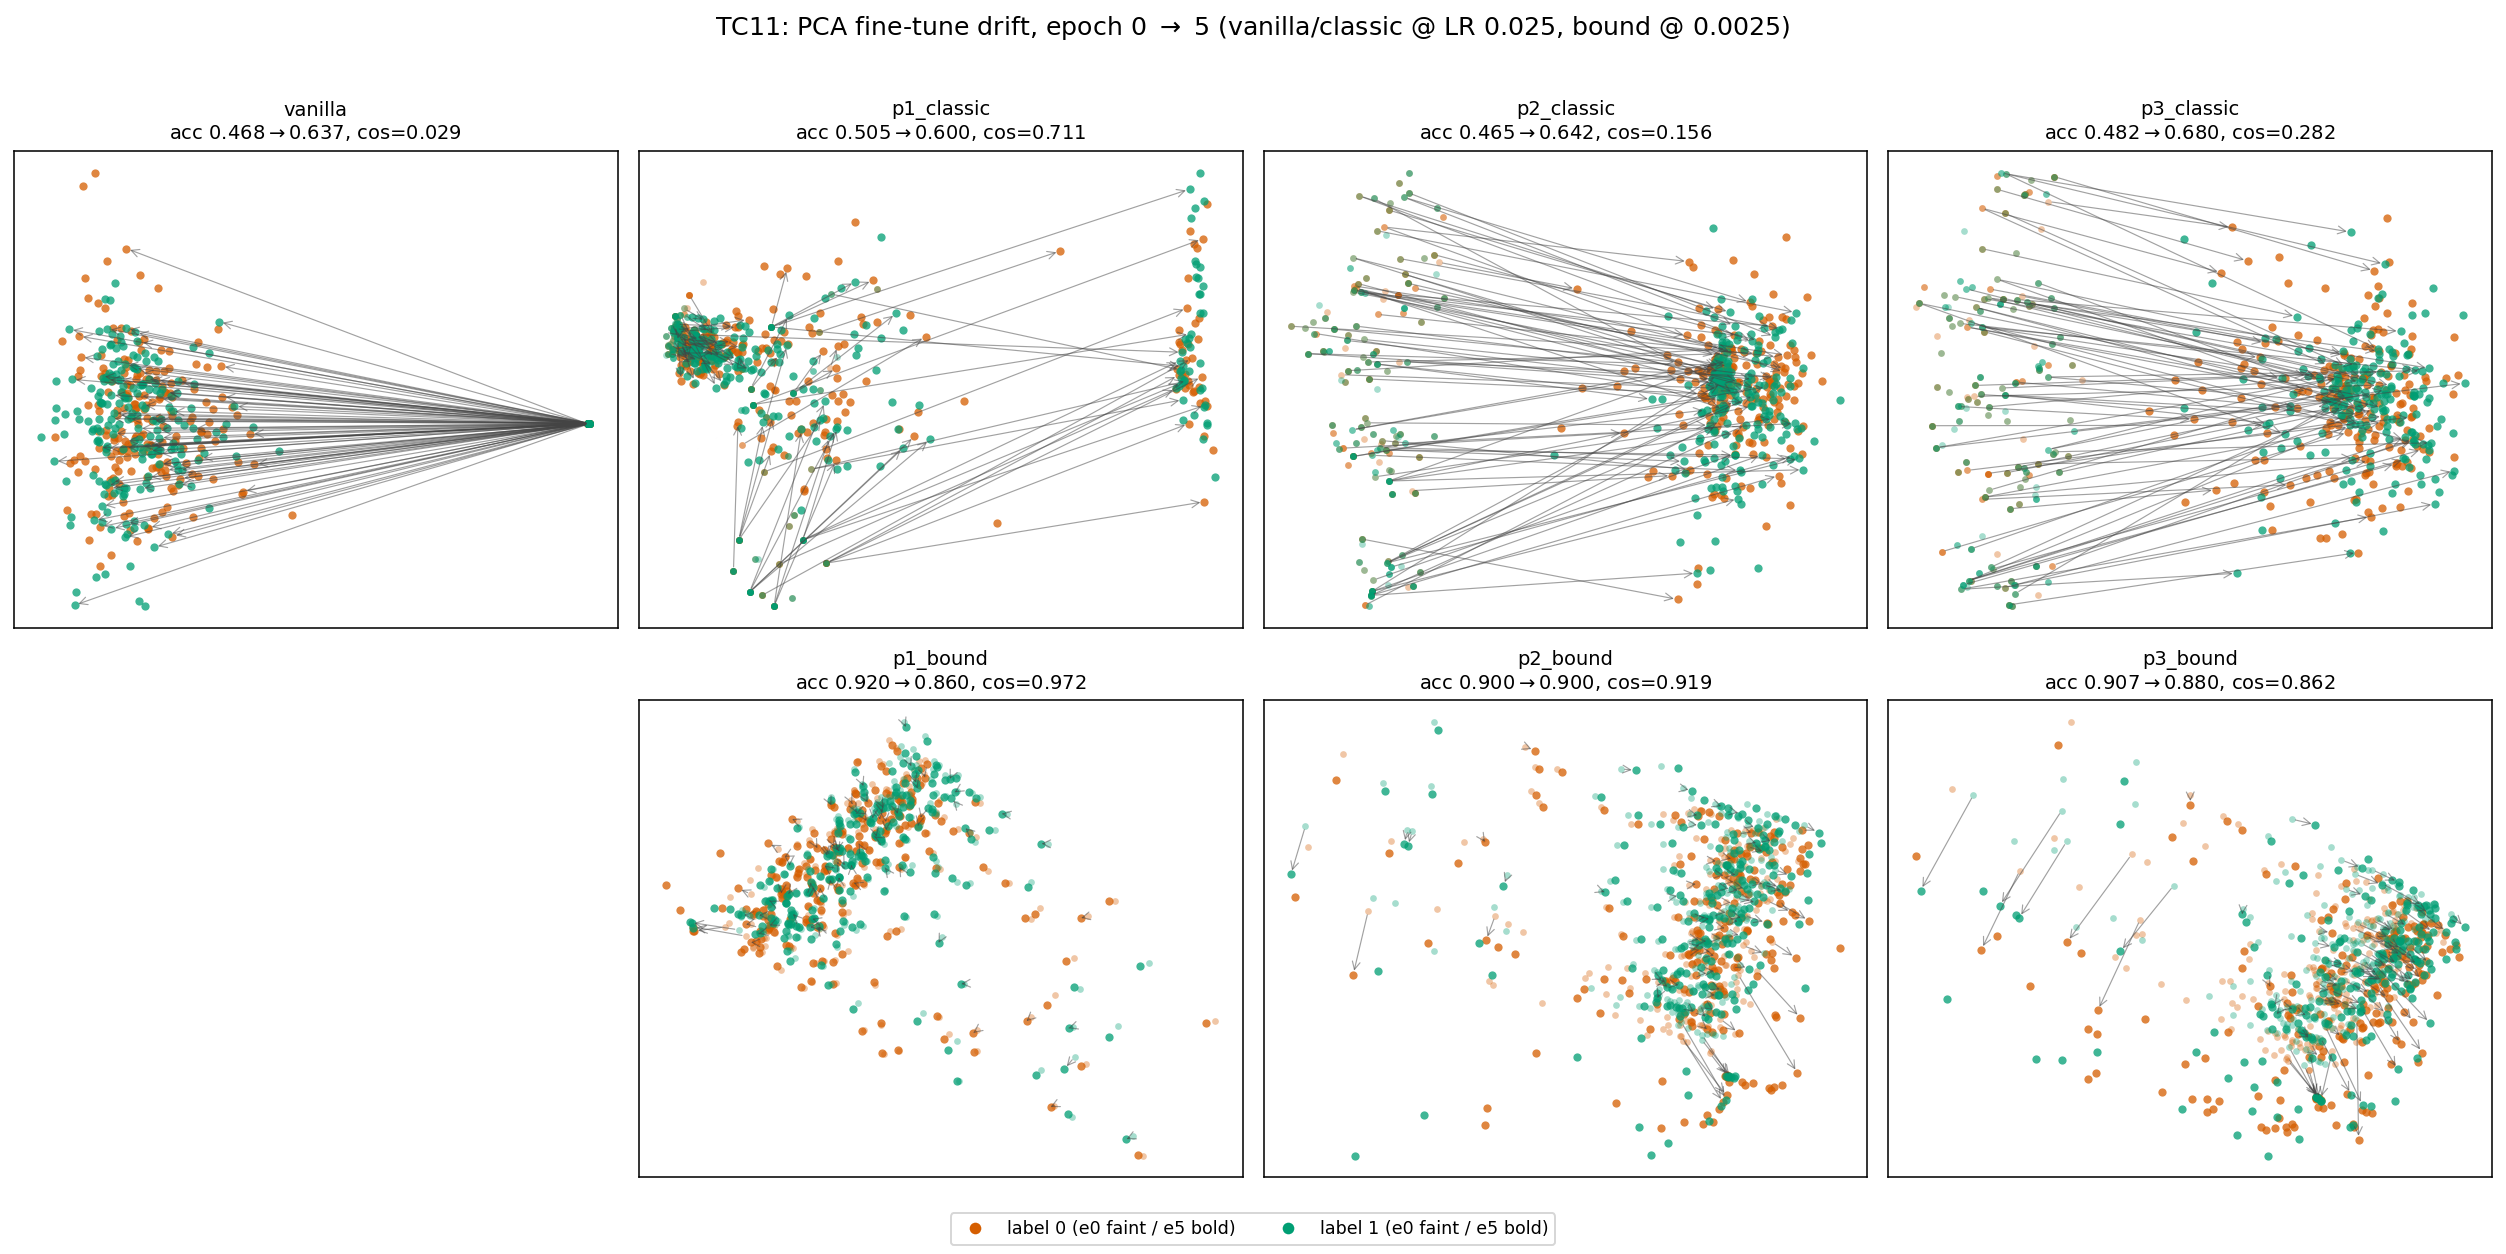
\includegraphics[width=\dimexpr\paperwidth-3cm\relax]{assets/pca_drift/tc11_pca_drift.png}} \\[1.0em]

  \makebox[\linewidth][c]{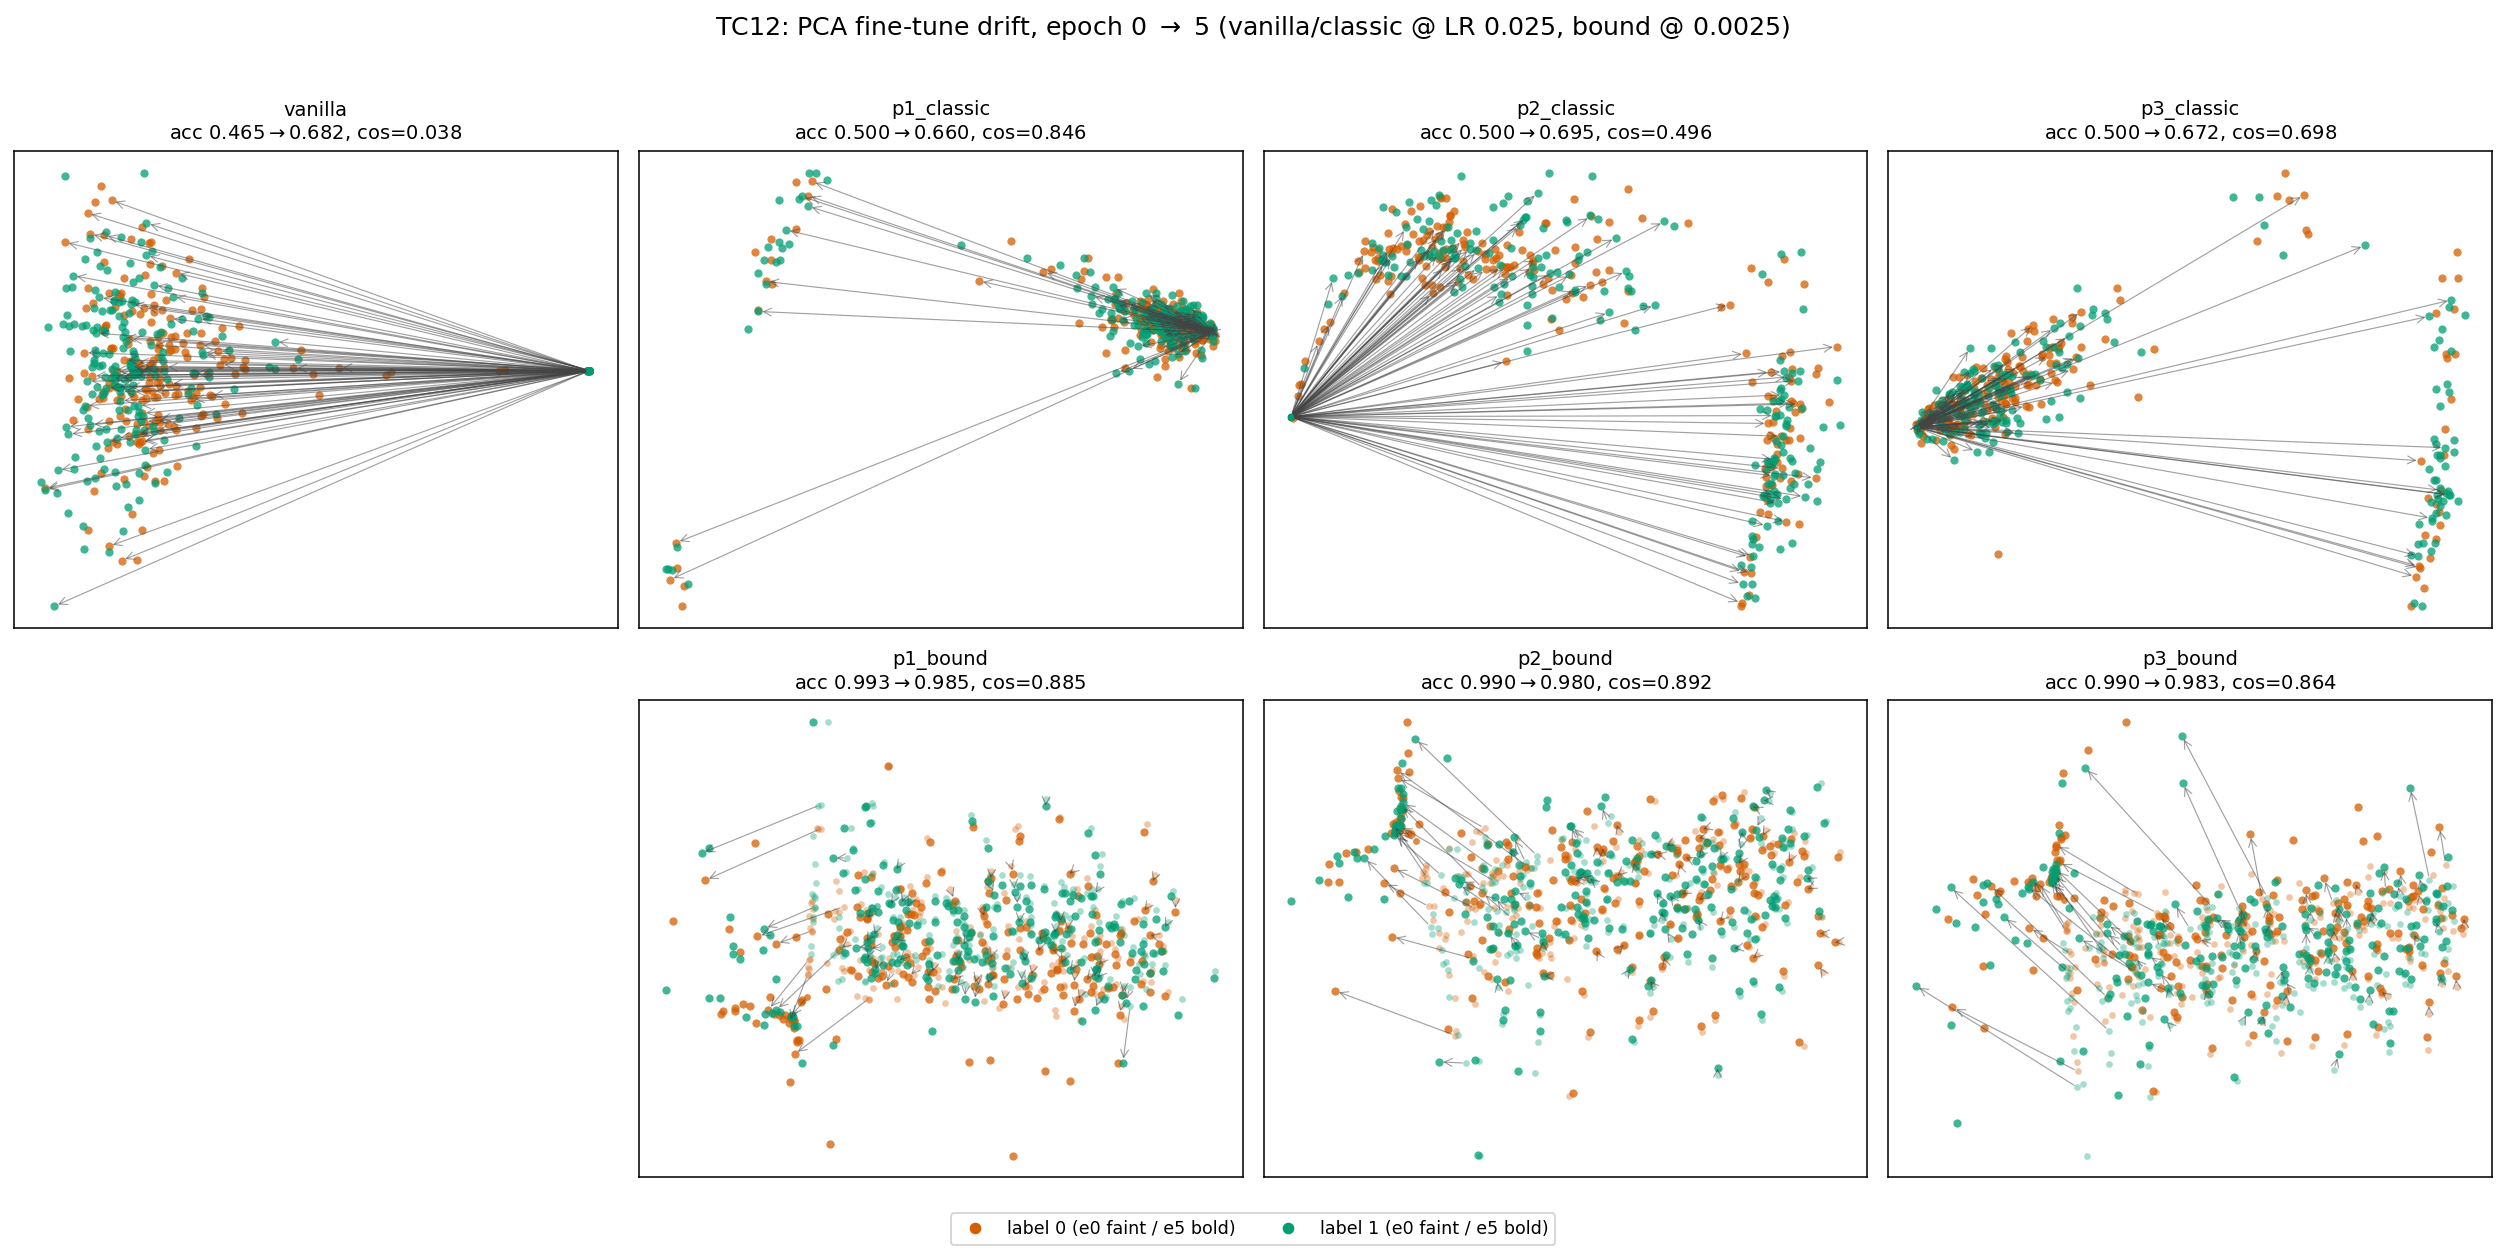
\includegraphics[width=\dimexpr\paperwidth-3cm\relax]{assets/pca_drift/tc12_pca_drift.png}} \\[1.0em]

  \makebox[\linewidth][c]{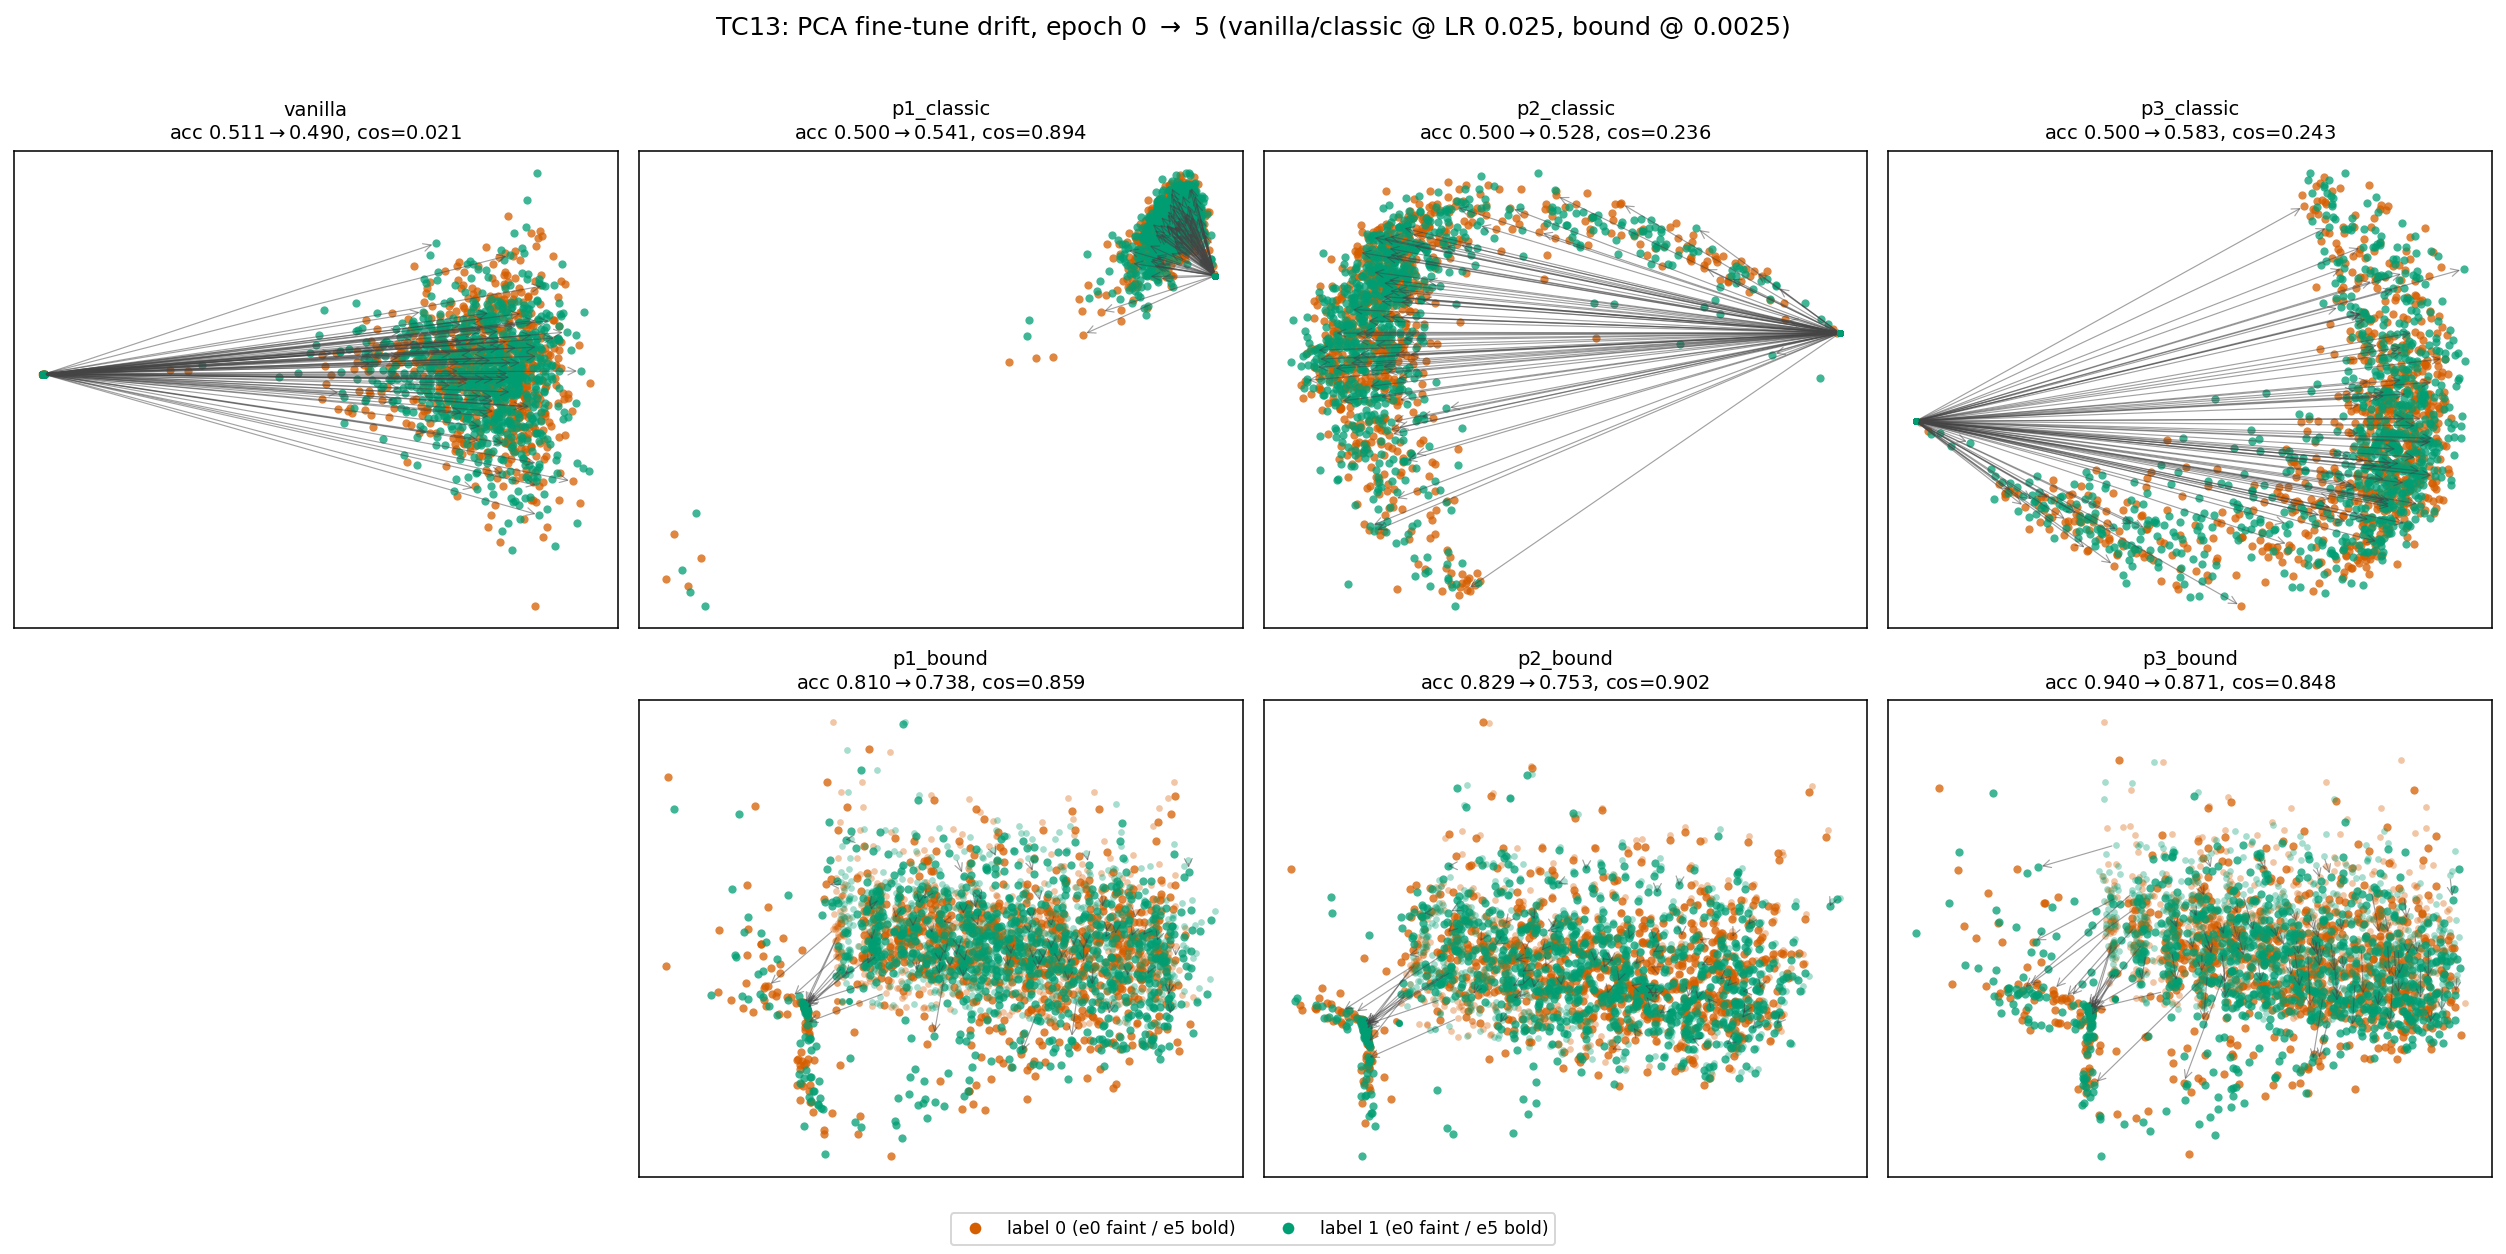
\includegraphics[width=\dimexpr\paperwidth-3cm\relax]{assets/pca_drift/tc13_pca_drift.png}} \\[1.0em]

  \makebox[\linewidth][c]{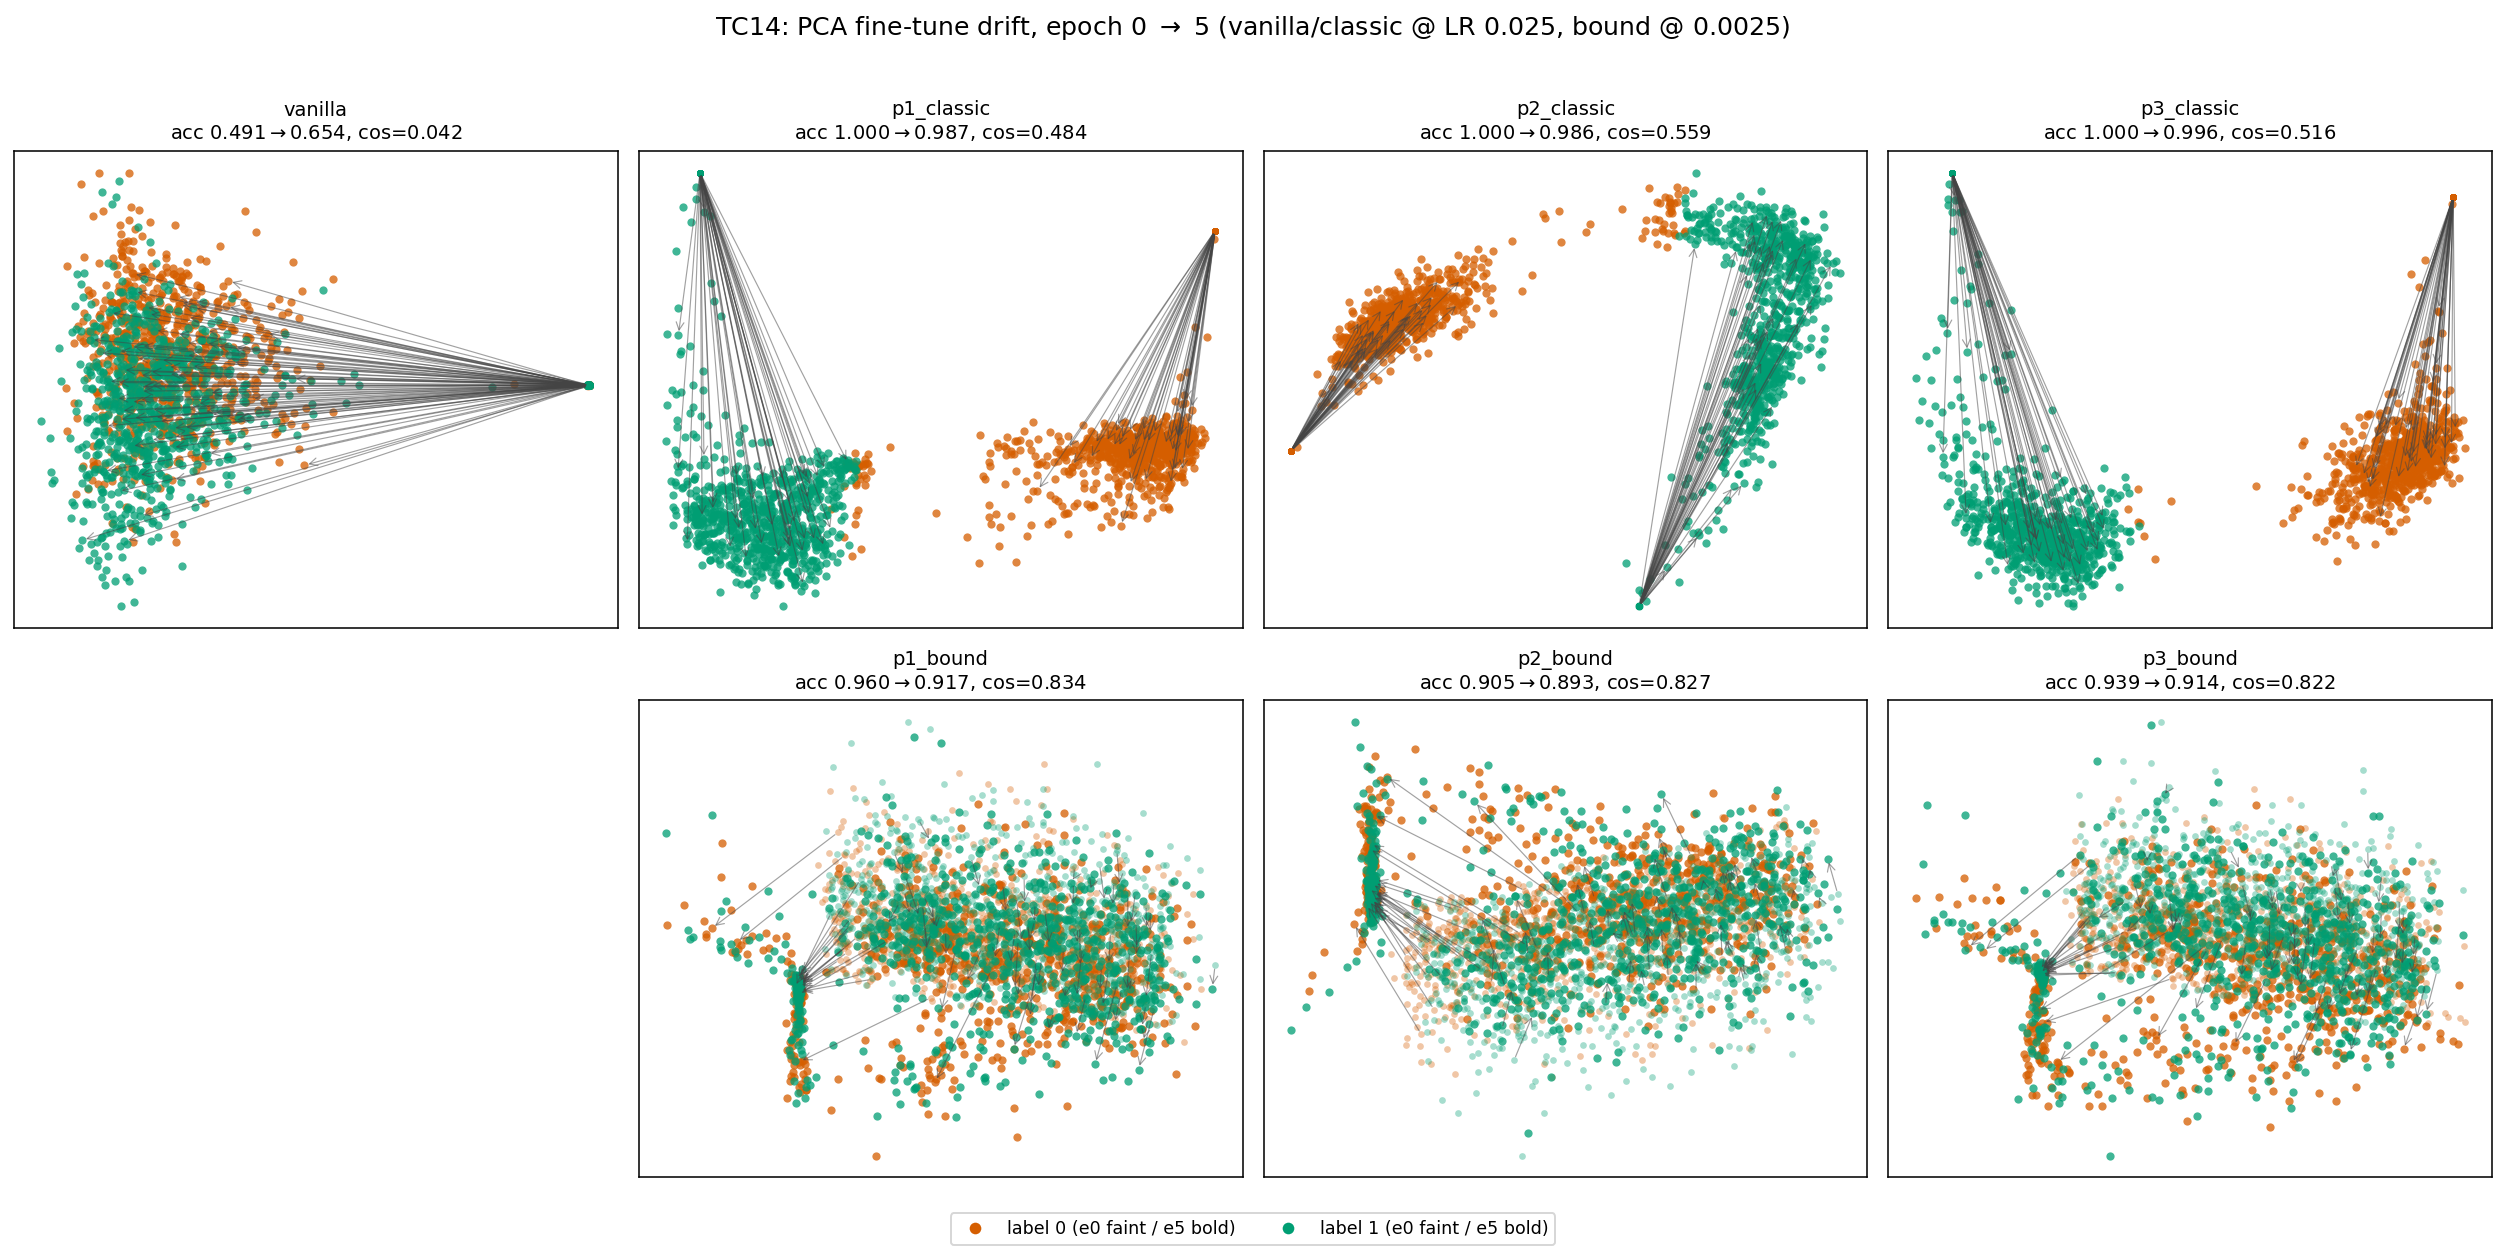
\includegraphics[width=\dimexpr\paperwidth-3cm\relax]{assets/pca_drift/tc14_pca_drift.png}} \\[1.0em]

  \makebox[\linewidth][c]{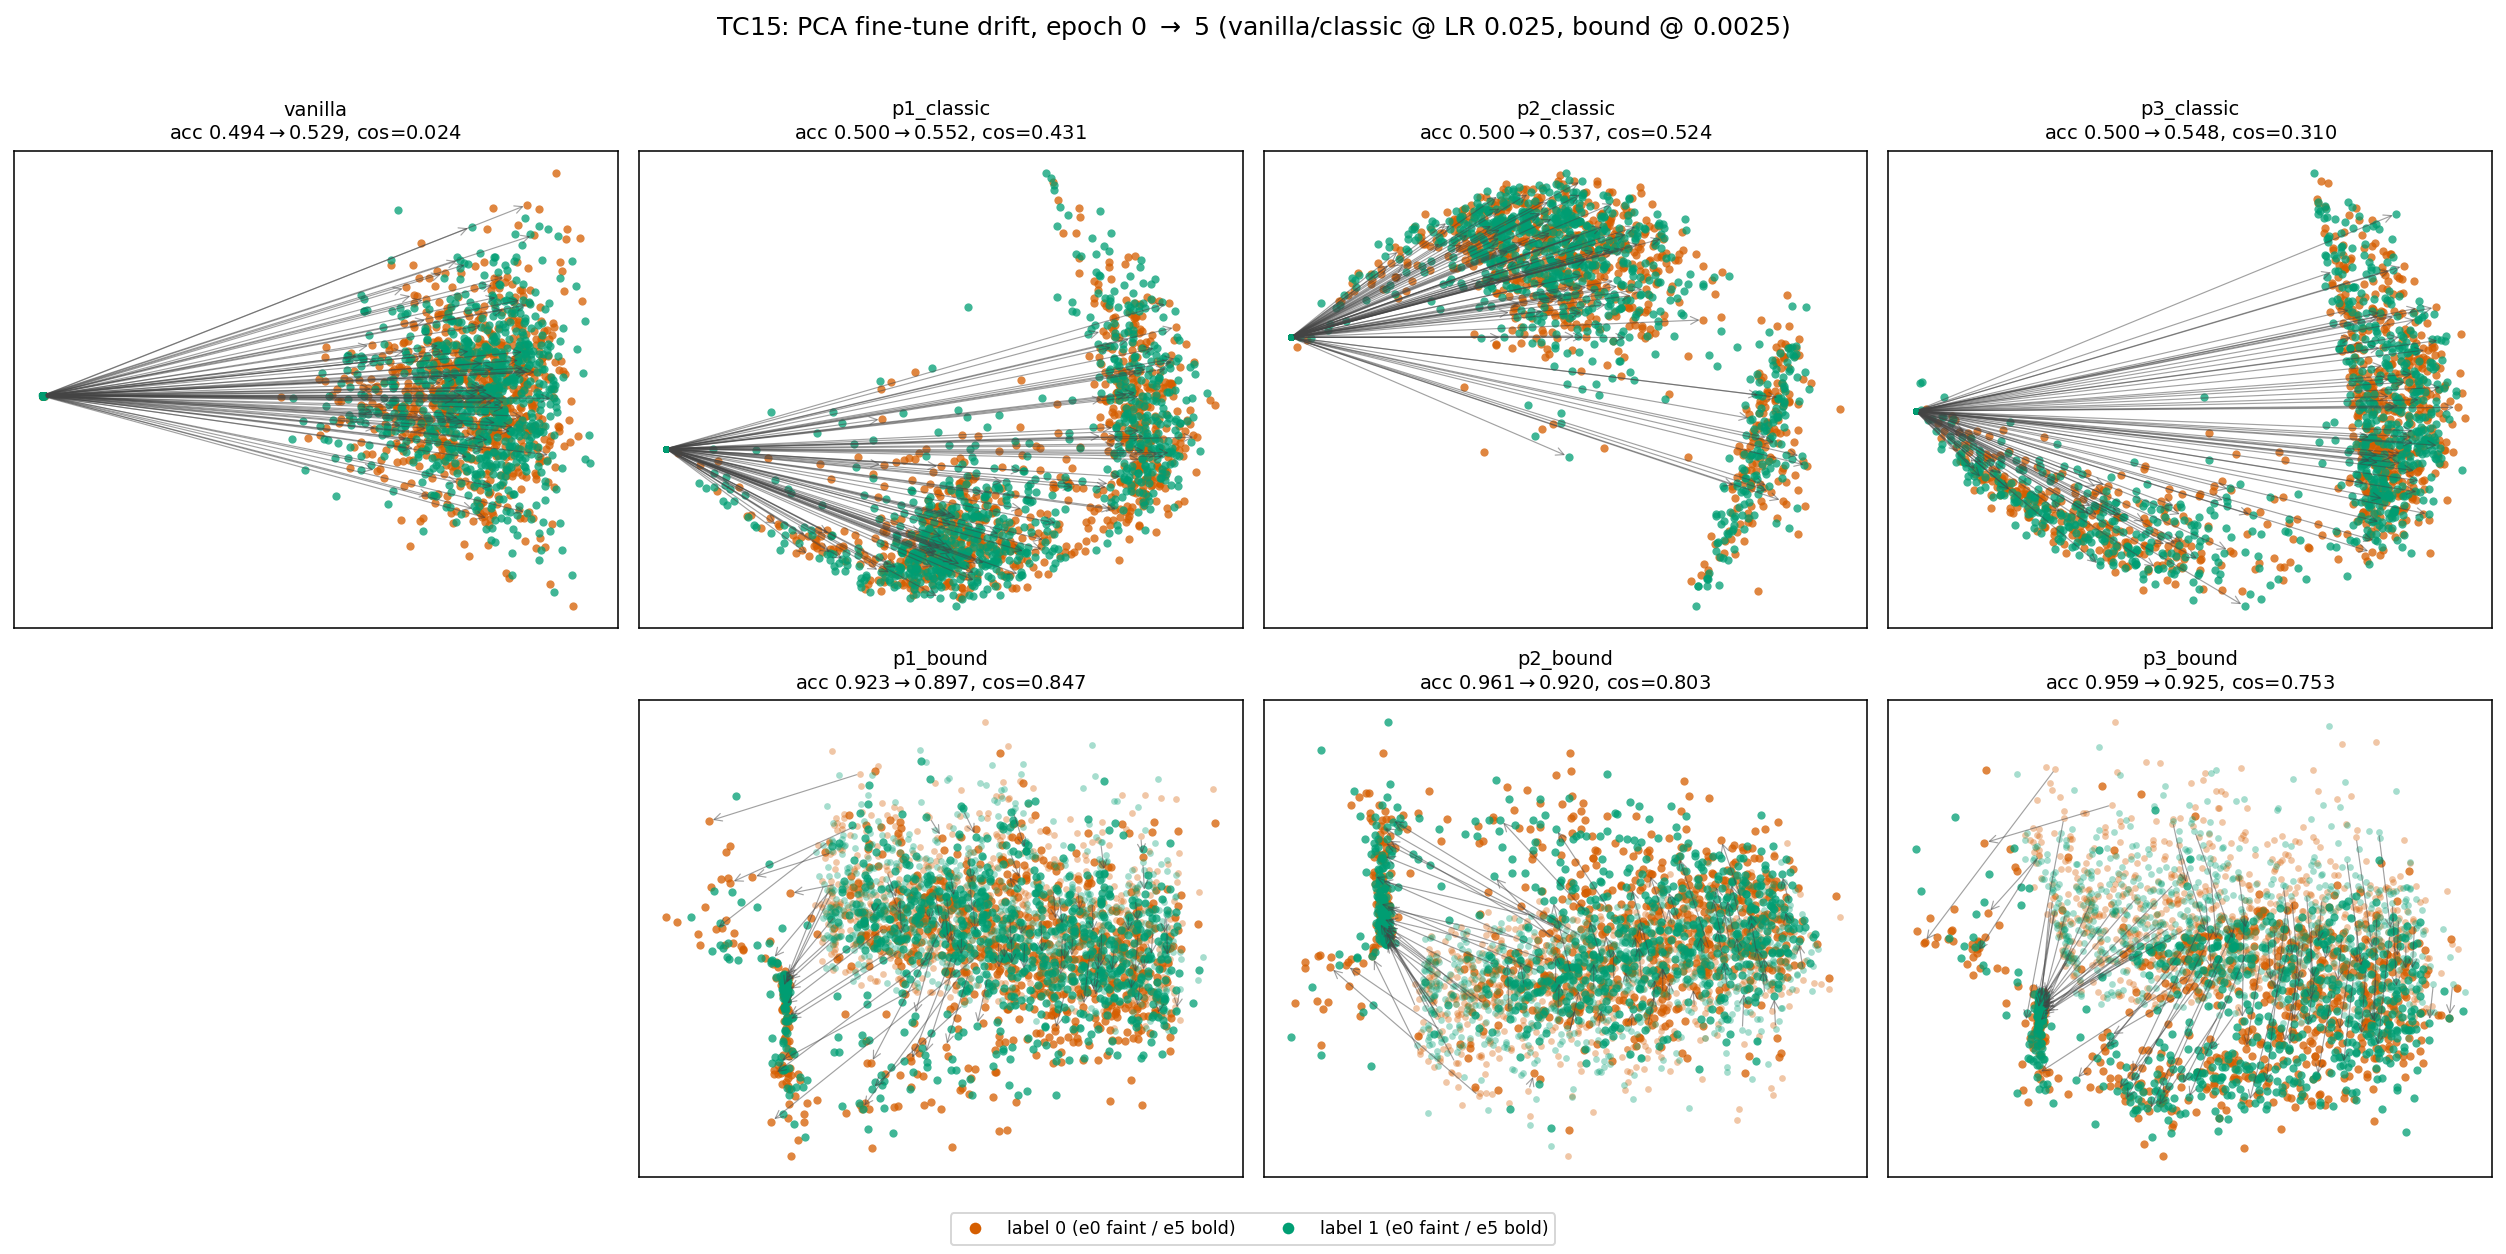
\includegraphics[width=\dimexpr\paperwidth-3cm\relax]{assets/pca_drift/tc15_pca_drift.png}}
  \end{longtable}
  \end{center}

\section{Embedding Drift (Cosine) for All Synthetic Test Cases}
\label{app:cosine-drift-all}

Figure~\ref{fig:embedding_drift_tc01_tc12} in Section~\ref{sec:results_drift}
reports the scalar embedding drift $1 - |\cos(\mathbf{v}_0, \mathbf{v}_t)|$ over
the fine-tuning epochs for the three representative test cases tc01, tc07 and
tc10. This appendix reproduces the same curves for the remaining twelve DLCC
synthetic test cases, confirming that the pattern holds across the whole
benchmark rather than only on the showcase cases: \texttt{vanilla} saturates to
near-full drift within a single epoch, the classic transfers drift
early and then plateau, and the concept-bound variants under the protected
learning rate stay low throughout. The curves are rendered from the per-epoch
entity-vector checkpoints of the same runs reported in
Table~\ref{tab:synthetic_final}, so they reflect exactly those runs rather than a
separate re-training.

\begin{figure}[p]
    \centering

    \begin{minipage}[t]{0.32\textwidth}
        \centering
        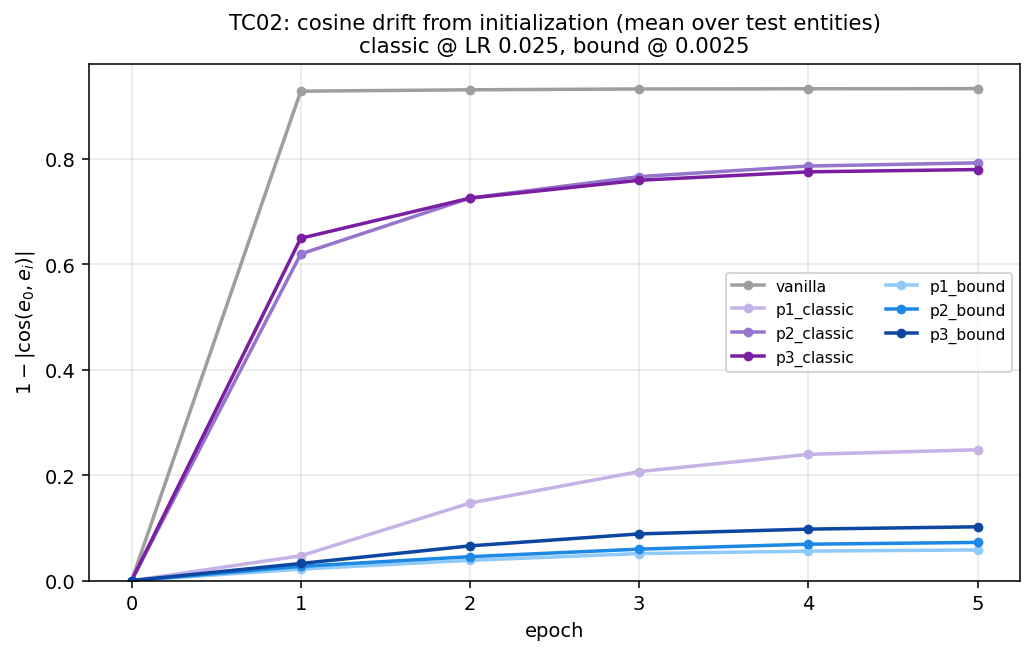
\includegraphics[width=\linewidth]{assets/cosine_drift/tc02_cosine_drift.png}
    \end{minipage}
    \hfill
    \begin{minipage}[t]{0.32\textwidth}
        \centering
        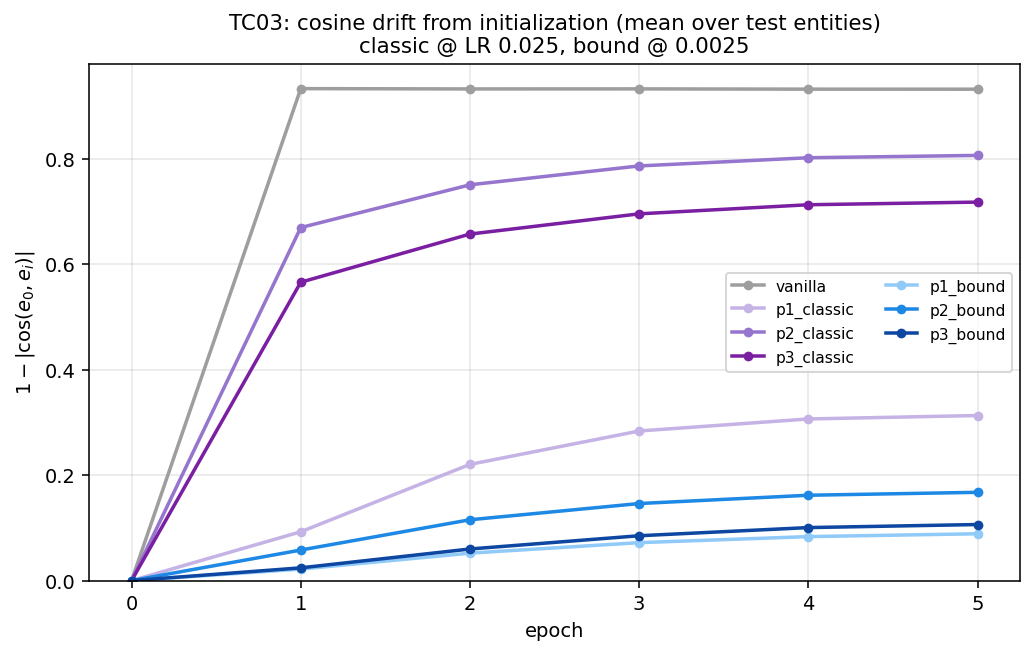
\includegraphics[width=\linewidth]{assets/cosine_drift/tc03_cosine_drift.png}
    \end{minipage}
    \hfill
    \begin{minipage}[t]{0.32\textwidth}
        \centering
        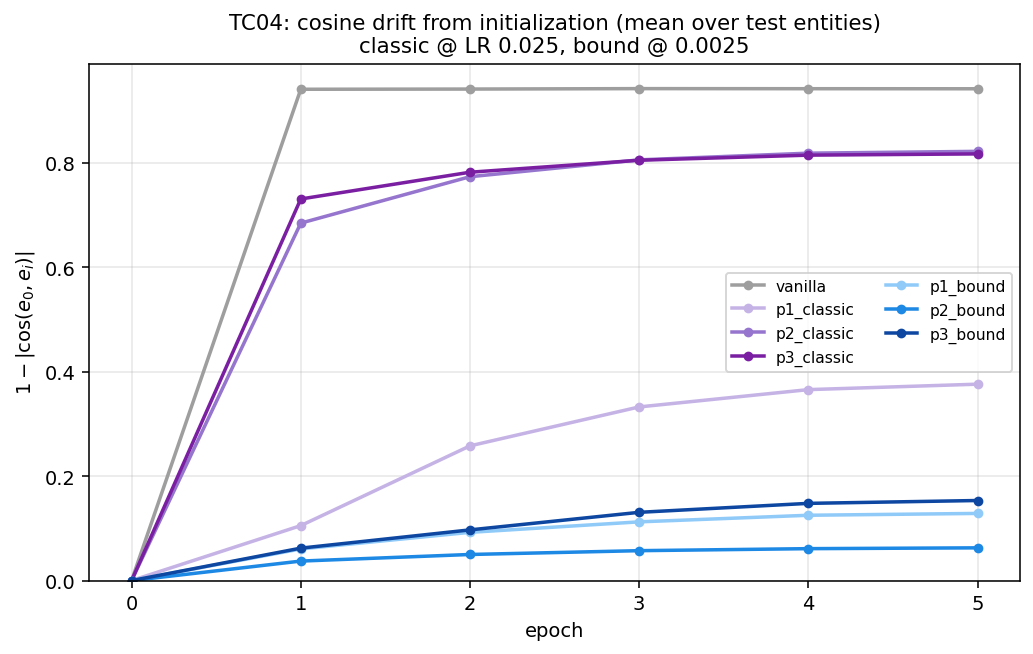
\includegraphics[width=\linewidth]{assets/cosine_drift/tc04_cosine_drift.png}
    \end{minipage}

    \vspace{0.8em}

    \begin{minipage}[t]{0.32\textwidth}
        \centering
        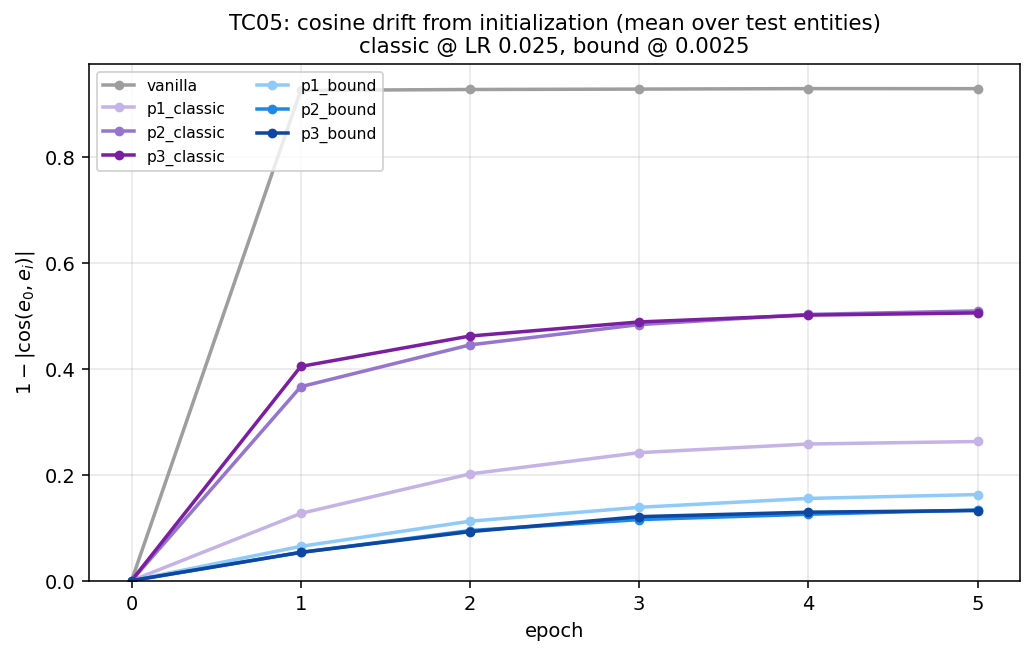
\includegraphics[width=\linewidth]{assets/cosine_drift/tc05_cosine_drift.png}
    \end{minipage}
    \hfill
    \begin{minipage}[t]{0.32\textwidth}
        \centering
        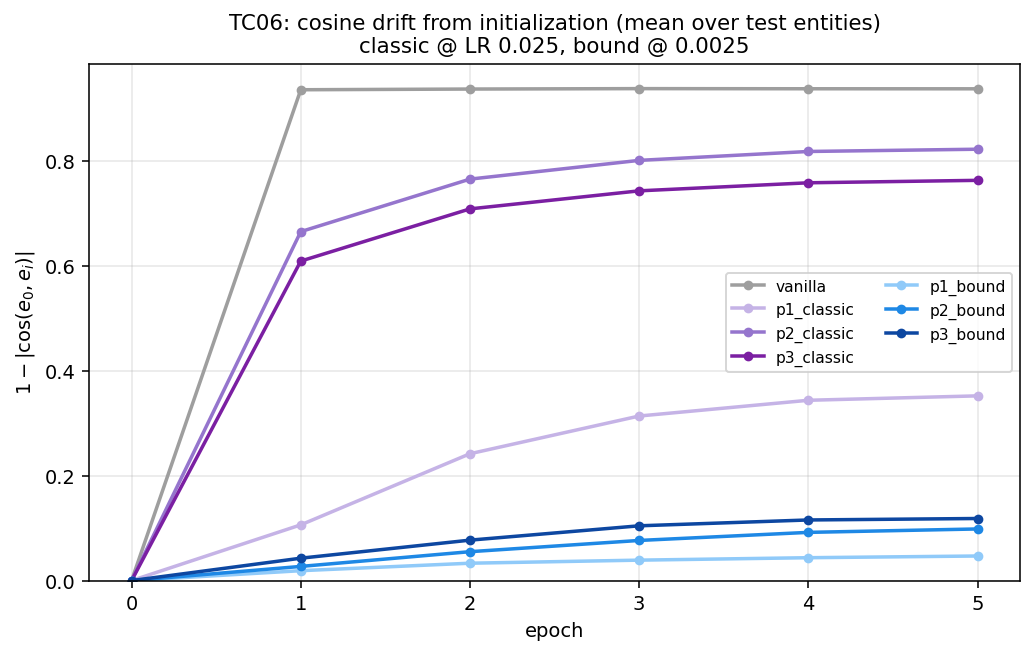
\includegraphics[width=\linewidth]{assets/cosine_drift/tc06_cosine_drift.png}
    \end{minipage}
    \hfill
    \begin{minipage}[t]{0.32\textwidth}
        \centering
        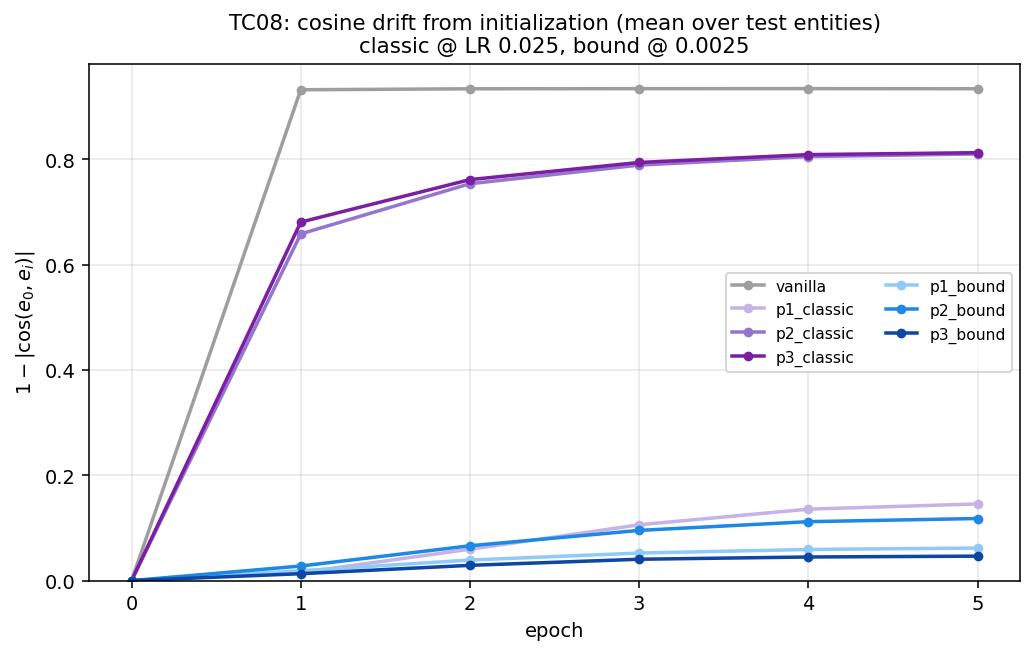
\includegraphics[width=\linewidth]{assets/cosine_drift/tc08_cosine_drift.png}
    \end{minipage}

    \vspace{0.8em}

    \begin{minipage}[t]{0.32\textwidth}
        \centering
        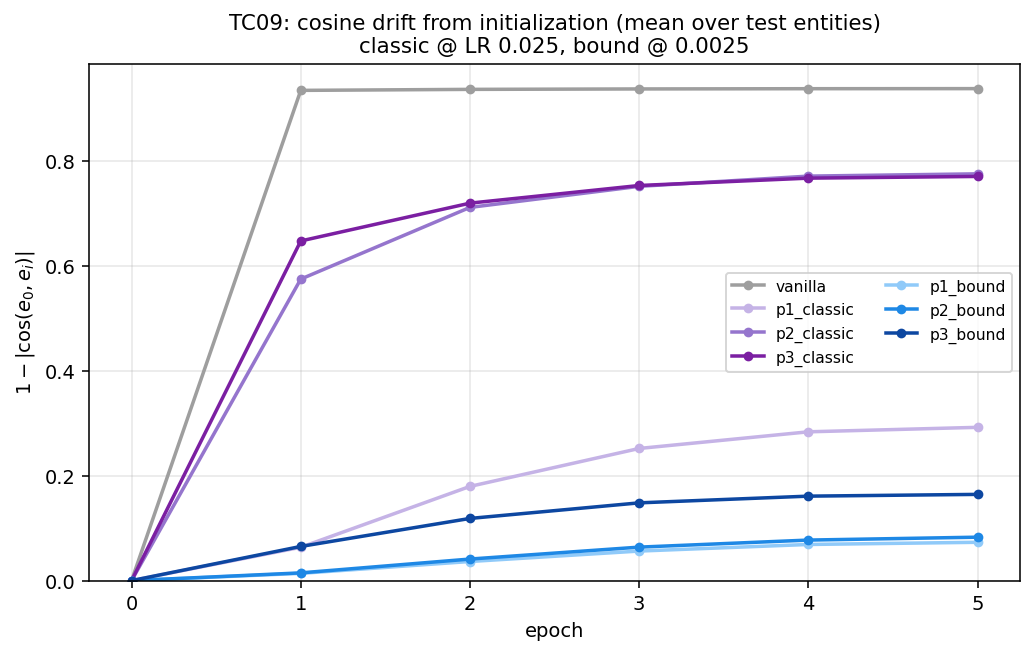
\includegraphics[width=\linewidth]{assets/cosine_drift/tc09_cosine_drift.png}
    \end{minipage}
    \hfill
    \begin{minipage}[t]{0.32\textwidth}
        \centering
        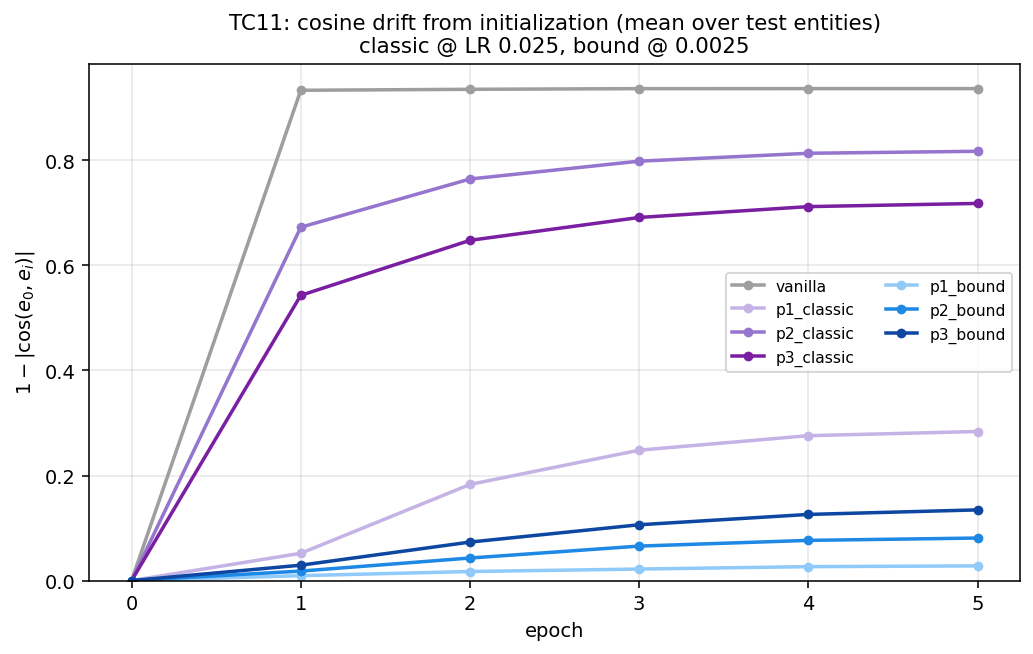
\includegraphics[width=\linewidth]{assets/cosine_drift/tc11_cosine_drift.png}
    \end{minipage}
    \hfill
    \begin{minipage}[t]{0.32\textwidth}
        \centering
        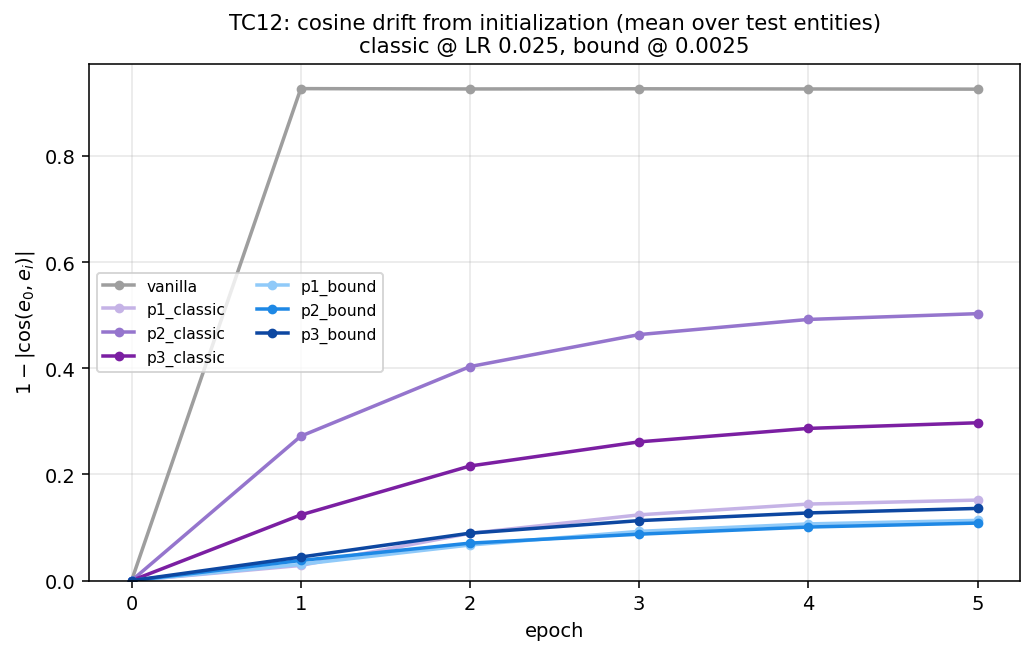
\includegraphics[width=\linewidth]{assets/cosine_drift/tc12_cosine_drift.png}
    \end{minipage}

    \vspace{0.8em}

    \begin{minipage}[t]{0.32\textwidth}
        \centering
        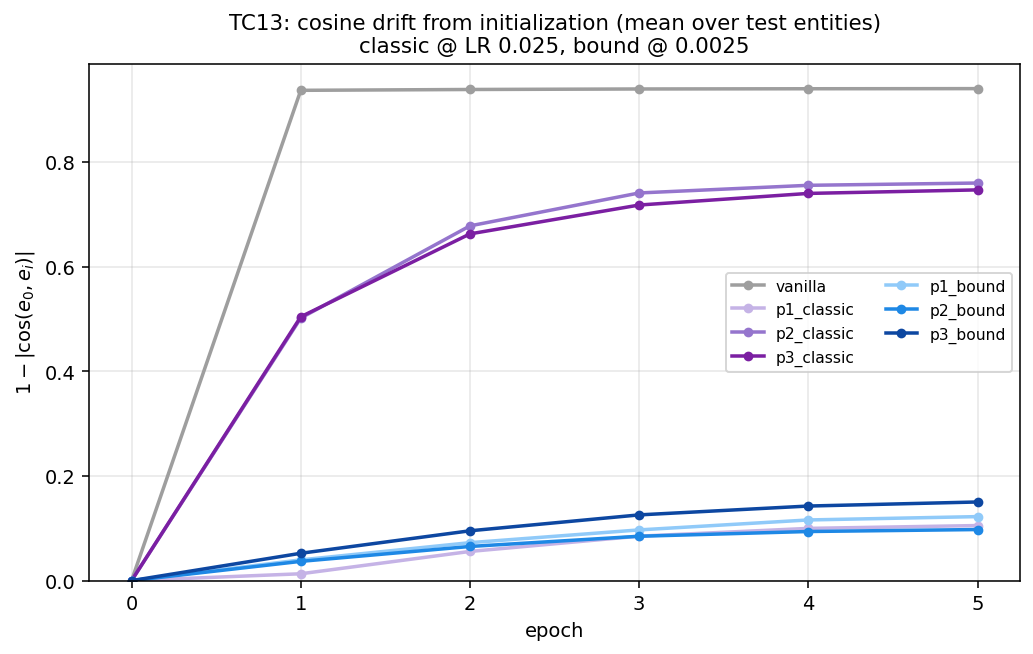
\includegraphics[width=\linewidth]{assets/cosine_drift/tc13_cosine_drift.png}
    \end{minipage}
    \hfill
    \begin{minipage}[t]{0.32\textwidth}
        \centering
        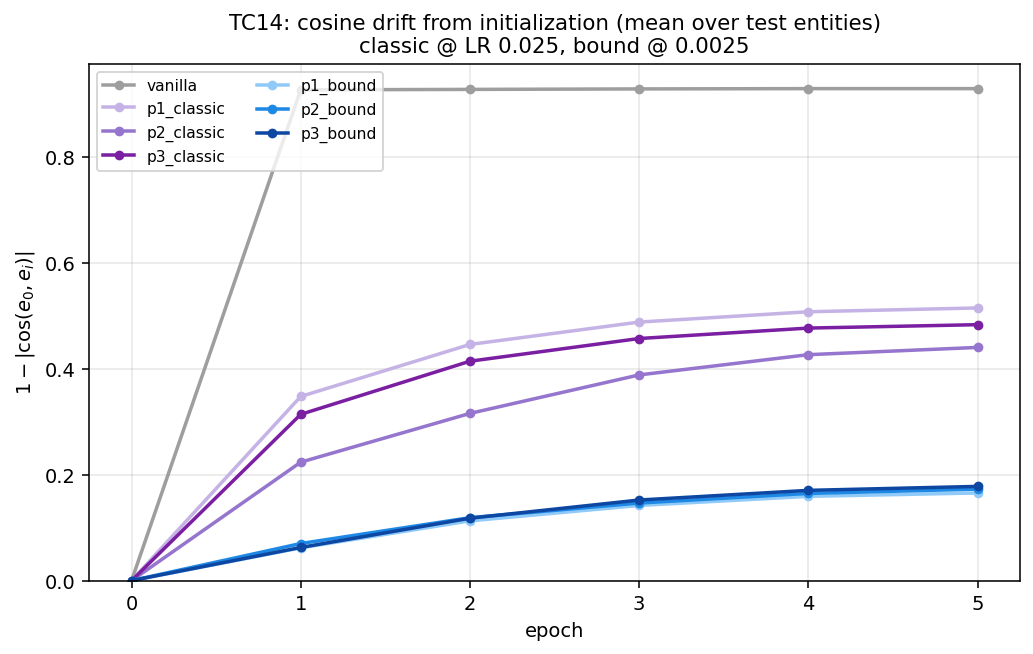
\includegraphics[width=\linewidth]{assets/cosine_drift/tc14_cosine_drift.png}
    \end{minipage}
    \hfill
    \begin{minipage}[t]{0.32\textwidth}
        \centering
        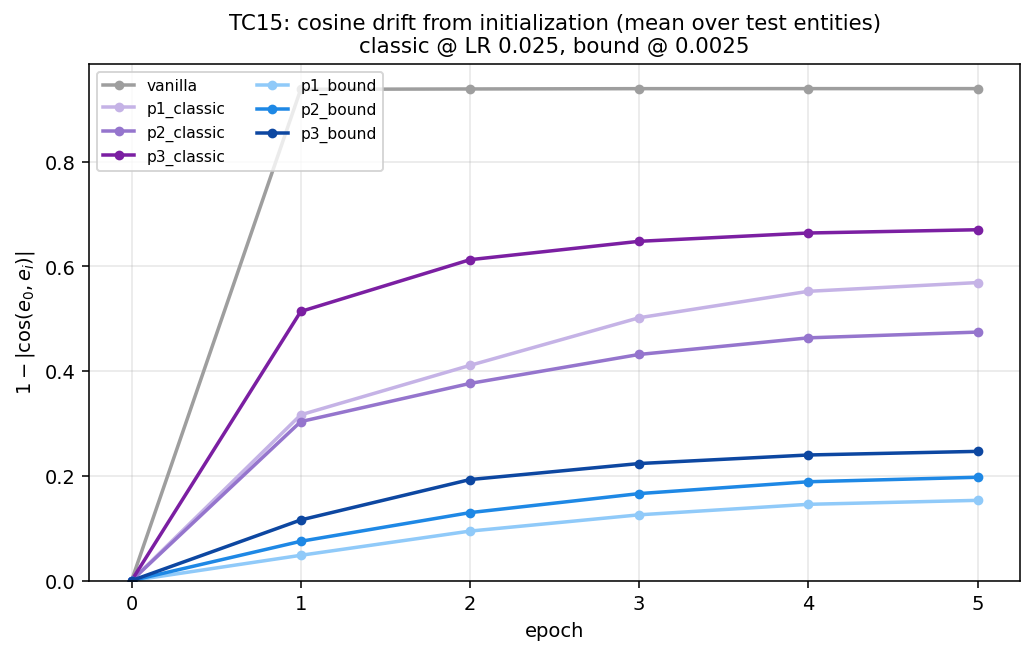
\includegraphics[width=\linewidth]{assets/cosine_drift/tc15_cosine_drift.png}
    \end{minipage}

    \caption{Embedding drift over fine-tuning epochs for all seven variants on the remaining twelve DLCC synthetic test cases (tc02--tc06, tc08, tc09 and tc11--tc15); the representative cases tc01, tc07 and tc10 are shown in Figure~\ref{fig:embedding_drift_tc01_tc12}. Drift is measured as $1 - |\cos(\mathbf{v}_0, \mathbf{v}_t)|$, where $\mathbf{v}_0$ is the initial embedding and $\mathbf{v}_t$ is the embedding after fine-tuning epoch $t$. The classic variants use the from-scratch learning rate $0.025$ and the concept-bound variants the protected rate $0.0025$.}
    \label{fig:embedding_drift_appendix}
\end{figure}

\section{Direction-Tag Ablation Across All Directional Test Cases}
\label{app:direction-all}

Table~\ref{tab:direction_pipeline} in Section~\ref{sec:results_direction}
reports the direction-tag ablation for the P2 protograph initialization on the
cardinality test cases tc09--tc12. Table~\ref{tab:direction_all} extends it to
all six directional test cases -- the existence controls tc01/tc02 and the
cardinality pairs tc09/tc10 and tc11/tc12 -- and averages each method over the
three protograph initializations, so each cell is the mean final accuracy of
that method across the \texttt{p1\_bound}, \texttt{p2\_bound} and
\texttt{p3\_bound} recipes. As in the main text, \textbf{no card.} is the
count-free, direction-agnostic baseline and the four tagged columns add the
cardinality count term back with the named direction tag on the incoming-edge
code. The full grid is produced by \texttt{scripts/\_direction\_grid.py} and
rendered in \texttt{notebooks/direction\_aware\_cardinality.ipynb} (Part~D).

\begin{table}[ht]
\centering
\small
\caption{Direction-tag ablation across all six directional test cases, full
pipeline. Each cell is the final test accuracy after 5 protected fine-tuning
epochs, averaged over the P1/P2/P3 protograph initializations. \textbf{no card.}
is the concept-bound initialization without the cardinality count term
($\delta{=}0$, direction-blind binding); the remaining columns add that count
term back with the corresponding direction tag. Best per row in bold.}
\label{tab:direction_all}
\begin{tabular}{lccccc}
\toprule
\textbf{TC} & \textbf{no card.} & \textbf{shared} & \textbf{rolled} & \textbf{negated} & \textbf{keyed} \\
\midrule
tc01 & 0.925 & 0.941 & 0.962 & 0.918 & \textbf{0.963} \\
tc02 & 0.944 & 0.951 & \textbf{0.974} & 0.959 & 0.973 \\
tc09 & 0.726 & 0.751 & \textbf{0.833} & 0.784 & \textbf{0.833} \\
tc10 & 0.721 & 0.728 & \textbf{0.808} & 0.725 & 0.785 \\
tc11 & 0.842 & 0.866 & \textbf{0.894} & 0.828 & 0.887 \\
tc12 & 0.961 & 0.966 & \textbf{0.987} & 0.952 & 0.979 \\
\midrule
Mean & 0.853 & 0.867 & \textbf{0.910} & 0.861 & 0.903 \\
\bottomrule
\end{tabular}
\end{table}

\section{Initialization-Strategy Comparison: Full Results}
\label{app:init-strategies}

Table~\ref{tab:init_strategies_pertc} gives the complete per-test-case results
behind the initialization-strategy comparison of
Section~\ref{sec:results_init_strategies} (Table~\ref{tab:init_strategies}):
final Logistic Regression test accuracy on the fifteen synthetic test cases
\texttt{tc01}--\texttt{tc15} for the four class-hierarchy initialization
strategies (\texttt{most\_specific}, \texttt{all\_init}, \texttt{average\_hier},
\texttt{weight\_hierarchy}) on each protograph transfer (P1, P2, P3), together
with the from-scratch \texttt{vanilla} baseline. The best strategy in each row is
in bold and the bottom row, the mean over the fifteen test cases, reproduces the
\texttt{Acc@final} column of Table~\ref{tab:init_strategies}.

\begin{table}[p]
\centering
\footnotesize
\setlength{\tabcolsep}{3pt}
\caption{Per-test-case final LogReg test accuracy (epoch~5) for the four class-hierarchy initialization strategies on each protograph: the full breakdown behind the \texttt{Acc@final} column of Table~\ref{tab:init_strategies} (same fixed budget: $\dim=200$, 100 instance walks/entity, depth~3, $5{+}5$ epochs, $\lambda=0.5$, from-scratch fine-tuning rate $0.025$; single run per cell). Strategies are abbreviated \texttt{ms}~(\texttt{most\_specific}), \texttt{ai}~(\texttt{all\_init}), \texttt{ah}~(\texttt{average\_hier}), \texttt{wh}~(\texttt{weight\_hierarchy}); \texttt{van} is the from-scratch \texttt{vanilla} baseline (protograph-independent, identical across the three groups). The best of the twelve strategy cells in each row is in bold; the bottom row is the mean over the fifteen test cases and reproduces the \texttt{Acc@final} column of Table~\ref{tab:init_strategies}.}
\label{tab:init_strategies_pertc}
\begin{tabular}{l r *{4}{r} *{4}{r} *{4}{r}}
\toprule
 & & \multicolumn{4}{c}{P1} & \multicolumn{4}{c}{P2} & \multicolumn{4}{c}{P3} \\
\cmidrule(lr){3-6}\cmidrule(lr){7-10}\cmidrule(lr){11-14}
TC & \texttt{van} & \texttt{ms} & \texttt{ai} & \texttt{ah} & \texttt{wh} & \texttt{ms} & \texttt{ai} & \texttt{ah} & \texttt{wh} & \texttt{ms} & \texttt{ai} & \texttt{ah} & \texttt{wh} \\
\midrule
\texttt{tc01} & 0.963 & 0.922 & 0.495 & 0.477 & 0.477 & 0.910 & 0.905 & 0.905 & 0.925 & \textbf{0.935} & 0.922 & 0.535 & 0.927 \\
\texttt{tc02} & 0.845 & 0.858 & 0.685 & 0.445 & 0.443 & 0.858 & 0.833 & 0.485 & \textbf{0.877} & 0.850 & 0.843 & 0.480 & 0.868 \\
\texttt{tc03} & 0.945 & \textbf{0.932} & 0.485 & 0.492 & 0.492 & 0.925 & 0.930 & 0.500 & 0.777 & 0.693 & 0.710 & 0.492 & 0.522 \\
\texttt{tc04} & 1.000 & 0.993 & 0.995 & 0.750 & 0.795 & 0.995 & 0.995 & 0.988 & \textbf{1.000} & 0.998 & 0.995 & 0.995 & 0.998 \\
\texttt{tc05} & 0.858 & 0.943 & 0.927 & 0.935 & 0.938 & 0.925 & 0.938 & 0.932 & 0.935 & 0.948 & \textbf{0.950} & 0.938 & 0.938 \\
\texttt{tc06} & 0.985 & 0.828 & 0.487 & 0.432 & 0.487 & 0.978 & \textbf{0.980} & 0.713 & 0.975 & 0.975 & 0.965 & 0.500 & 0.978 \\
\texttt{tc07} & 0.583 & 0.535 & 0.485 & 0.482 & 0.482 & \textbf{0.610} & 0.535 & 0.468 & 0.547 & 0.502 & 0.525 & 0.490 & 0.485 \\
\texttt{tc08} & 0.595 & 0.530 & 0.505 & 0.495 & 0.500 & \textbf{0.542} & \textbf{0.542} & 0.500 & 0.512 & 0.465 & 0.505 & 0.525 & 0.540 \\
\texttt{tc09} & 0.657 & 0.632 & 0.450 & 0.460 & 0.470 & 0.632 & 0.640 & 0.477 & \textbf{0.680} & 0.623 & 0.625 & 0.460 & 0.470 \\
\texttt{tc10} & 0.660 & 0.647 & \textbf{0.688} & 0.535 & 0.530 & 0.667 & 0.662 & 0.500 & 0.635 & 0.670 & \textbf{0.688} & 0.470 & 0.470 \\
\texttt{tc11} & 0.603 & 0.625 & 0.490 & 0.470 & 0.495 & 0.660 & 0.642 & 0.642 & 0.615 & \textbf{0.680} & 0.677 & 0.450 & 0.472 \\
\texttt{tc12} & 0.672 & 0.675 & 0.500 & 0.500 & 0.500 & 0.677 & 0.660 & 0.502 & \textbf{0.682} & 0.680 & 0.675 & 0.500 & 0.527 \\
\texttt{tc13} & 0.525 & 0.544 & 0.506 & 0.500 & 0.500 & \textbf{0.553} & 0.527 & 0.496 & 0.494 & 0.507 & 0.514 & 0.514 & 0.517 \\
\texttt{tc14} & 0.662 & \textbf{1.000} & \textbf{1.000} & \textbf{1.000} & \textbf{1.000} & \textbf{1.000} & \textbf{1.000} & \textbf{1.000} & \textbf{1.000} & \textbf{1.000} & \textbf{1.000} & \textbf{1.000} & \textbf{1.000} \\
\texttt{tc15} & 0.537 & 0.611 & \textbf{0.612} & 0.497 & 0.497 & 0.600 & 0.587 & 0.510 & 0.489 & 0.598 & 0.591 & 0.487 & 0.500 \\
\midrule
\textbf{mean} & 0.739 & 0.752 & 0.621 & 0.565 & 0.574 & 0.769 & 0.758 & 0.641 & 0.743 & 0.742 & 0.746 & 0.589 & 0.681 \\
\bottomrule
\end{tabular}
\end{table}


\section{Protograph Anchoring $\lambda$ Sweep: Full Results}
\label{app:anchoring-lambda}

Table~\ref{tab:anchoring_pertc_avg} gives the complete per-test-case results for
the protograph anchoring sweep summarized in
Figure~\ref{fig:anchoring_lambda_sweep} (Section~\ref{sec:results_anchoring}):
final Logistic Regression test accuracy on the fourteen synthetic test cases
\texttt{tc01}--\texttt{tc15} (excl.\ \texttt{tc04}) for the \texttt{vanilla}
baseline, the un-anchored transfer (\(\lambda=0\)) and every anchoring strength
\(\lambda\), averaged over the three protograph transfers (P1, P2, P3), with the
per-row best \(\lambda\) in bold and the mean over the fourteen test cases in the
bottom row.

\begin{table}[p]
\centering
\small
\caption{Per-test-case final LogReg test accuracy for the protograph anchoring sweep, \textbf{averaged over the three transfers P1, P2 and P3} (\texttt{most\_specific} initialization, normalized codes): \texttt{vanilla} baseline, the un-anchored transfer ($\lambda=0$), and each anchoring strength $\lambda$. Each cell is the mean of the corresponding P1/P2/P3 values (the \texttt{vanilla} baseline is identical across transfers). The best $\lambda$ value in each row is in bold; the bottom row is the mean over the fourteen test cases (\texttt{tc01}--\texttt{tc15}, excl.\ \texttt{tc04}).}
\label{tab:anchoring_pertc_avg}
\begin{tabular}{l r rrrrrr}
\toprule
 & & \multicolumn{6}{c}{anchoring strength $\lambda$} \\
\cmidrule(lr){3-8}
TC & \texttt{vanilla} & $0$ & $0.1$ & $0.25$ & $0.5$ & $0.75$ & $1.0$ \\
\midrule
\texttt{tc01} & 0.943 & \textbf{0.950} & 0.947 & 0.947 & 0.926 & 0.830 & 0.584 \\
\texttt{tc02} & 0.843 & \textbf{0.868} & 0.853 & 0.848 & 0.804 & 0.678 & 0.540 \\
\texttt{tc03} & 0.930 & \textbf{0.928} & 0.922 & 0.919 & 0.888 & 0.775 & 0.578 \\
\texttt{tc05} & 0.830 & 0.938 & 0.937 & \textbf{0.944} & 0.942 & 0.927 & 0.930 \\
\texttt{tc06} & 0.983 & \textbf{0.984} & \textbf{0.984} & \textbf{0.984} & 0.970 & 0.888 & 0.599 \\
\texttt{tc07} & 0.570 & 0.540 & \textbf{0.560} & 0.543 & 0.542 & 0.526 & 0.501 \\
\texttt{tc08} & 0.610 & \textbf{0.565} & 0.563 & 0.553 & 0.542 & 0.531 & 0.517 \\
\texttt{tc09} & 0.642 & \textbf{0.624} & 0.623 & 0.607 & 0.600 & 0.578 & 0.525 \\
\texttt{tc10} & 0.637 & 0.650 & \textbf{0.653} & 0.632 & 0.633 & 0.588 & 0.513 \\
\texttt{tc11} & 0.637 & \textbf{0.635} & 0.607 & 0.604 & 0.577 & 0.541 & 0.499 \\
\texttt{tc12} & 0.677 & 0.673 & 0.676 & 0.660 & 0.673 & \textbf{0.681} & 0.633 \\
\texttt{tc13} & 0.510 & 0.559 & \textbf{0.562} & 0.551 & 0.560 & 0.546 & 0.500 \\
\texttt{tc14} & 0.671 & 0.991 & 0.997 & \textbf{1.000} & \textbf{1.000} & \textbf{1.000} & \textbf{1.000} \\
\texttt{tc15} & 0.510 & \textbf{0.567} & 0.560 & 0.560 & 0.532 & 0.525 & 0.521 \\
\midrule
\textbf{mean} & 0.714 & \textbf{0.748} & 0.746 & 0.740 & 0.728 & 0.687 & 0.603 \\
\bottomrule
\end{tabular}
\end{table}


\section{Fine-Tuning Learning-Rate Ablation: Full Results}
\label{app:lr-ablation}

Table~\ref{tab:lr_ablation} gives the complete per-test-case results for the
learning-rate ablation summarized in Figure~\ref{fig:lr_ablation}
(Section~\ref{sec:results_lr}): final Logistic Regression test accuracy on the
fifteen synthetic test cases \texttt{tc01}--\texttt{tc15} for each classic
(\texttt{all\_init}) transfer at the protected rate $0.0025$ and the
from-scratch rate $0.025$, together with the from-scratch \texttt{vanilla}
baseline. The bottom rows report the per-column mean and, for each transfer, the
change $\Delta$ when the rate is lowered from $0.025$ to $0.0025$.

\begin{table}[ht]
\centering
\small
\caption{Fine-tuning learning-rate ablation for the classic (\texttt{all\_init}) transfer on the synthetic DLCC test cases \texttt{tc01}--\texttt{tc15}, under the fixed comparison budget ($\dim=200$, 100 instance walks/entity, depth 3, $5+5$ epochs, codes normalized to $8$ and mirrored into \texttt{syn1neg}, seed 42). Each cell is the final LogReg test accuracy after the 5th fine-tuning epoch. \emph{0.0025} is the protected rate used by the concept-bound variants; \emph{0.025} is the from-scratch rate. The \texttt{vanilla} column (LR 0.025) is the from-scratch baseline. The 0.0025 columns are from \texttt{synthetic\_compare} (\texttt{p1}/\texttt{p2}) and the \texttt{p3\_classic} run; the 0.025 columns are from the synthetic benchmark (the \texttt{p1}/\texttt{p2} values match the reruns of Table~\ref{tab:synthetic_final} to within run-to-run noise).}
\label{tab:lr_ablation}
\begin{tabular}{l rr rr rr c}
\toprule
 & \multicolumn{2}{c}{\texttt{p1\_classic}} & \multicolumn{2}{c}{\texttt{p2\_classic}} & \multicolumn{2}{c}{\texttt{p3\_classic}} & vanilla \\
\cmidrule(lr){2-3}\cmidrule(lr){4-5}\cmidrule(lr){6-7}\cmidrule(lr){8-8}
TC & 0.0025 & 0.025 & 0.0025 & 0.025 & 0.0025 & 0.025 & 0.025 \\
\midrule
tc01 & 0.805 & 0.953 & 0.905 & 0.950 & 0.925 & 0.955 & 0.950 \\
tc02 & 0.530 & 0.838 & 0.848 & 0.855 & 0.850 & 0.843 & 0.868 \\
tc03 & 0.500 & 0.943 & 0.935 & 0.922 & 0.632 & 0.917 & 0.955 \\
tc04 & 0.787 & 0.998 & 0.993 & 1.000 & 0.993 & 1.000 & 1.000 \\
tc05 & 0.930 & 0.943 & 0.938 & 0.922 & 0.943 & 0.955 & 0.838 \\
tc06 & 0.505 & 0.978 & 0.983 & 0.983 & 0.970 & 0.985 & 0.983 \\
tc07 & 0.487 & 0.545 & 0.600 & 0.552 & 0.568 & 0.570 & 0.573 \\
tc08 & 0.510 & 0.530 & 0.515 & 0.585 & 0.485 & 0.578 & 0.593 \\
tc09 & 0.450 & 0.635 & 0.613 & 0.662 & 0.630 & 0.630 & 0.623 \\
tc10 & 0.515 & 0.662 & 0.662 & 0.657 & 0.657 & 0.700 & 0.665 \\
tc11 & 0.497 & 0.600 & 0.665 & 0.642 & 0.675 & 0.680 & 0.637 \\
tc12 & 0.537 & 0.660 & 0.650 & 0.695 & 0.693 & 0.672 & 0.682 \\
tc13 & 0.501 & 0.541 & 0.507 & 0.528 & 0.527 & 0.583 & 0.490 \\
tc14 & 1.000 & 0.987 & 1.000 & 0.986 & 1.000 & 0.996 & 0.654 \\
tc15 & 0.573 & 0.552 & 0.576 & 0.537 & 0.571 & 0.548 & 0.529 \\
\midrule
\textbf{Mean} & 0.609 & 0.758 & 0.759 & 0.765 & 0.741 & 0.774 & 0.736 \\
\midrule
$\Delta$ & \multicolumn{2}{c}{$-0.149$} & \multicolumn{2}{c}{$-0.006$} & \multicolumn{2}{c}{$-0.033$} & -- \\
\bottomrule
\end{tabular}
\end{table}


\section{Initialization Normalization Ablation: Full Results}
\label{app:norm-ablation}

Table~\ref{tab:ms-norm-vs-nonorm-acc} gives the complete per-test-case results
for the normalization ablation summarized in
Section~\ref{sec:results_norm_ablation}: final Logistic Regression test accuracy
on the fifteen synthetic test cases \texttt{tc01}--\texttt{tc15} for each classic
transfer (\texttt{p1\_classic}, \texttt{p2\_classic}, \texttt{p3\_classic};
\texttt{most\_specific}), under the normalized (norm $8$) initialization and the
raw class-mean initialization, with the per-test-case difference $\Delta$ for each
transfer. Both settings use the from-scratch fine-tuning rate $0.025$. Figure~\ref{fig:norm_ablation_loss_nonorm} shows the per-epoch loss
without the normalization, the counterpart of the normalized
Figure~\ref{fig:compare_epoch_loss_tc01_tc15} in the main text.

% most_specific init, norm=8 vs no-norm raw-mean, final-epoch test accuracy (wide format)
\begin{table}[ht]
\centering
\small
\caption{Final test accuracy under the normalized (norm$=8$) vs.\ no-norm raw-mean protograph initialization (\texttt{most\_specific}) for the classic transfers \texttt{p1\_classic}, \texttt{p2\_classic}, \texttt{p3\_classic} on the synthetic DLCC test cases \texttt{tc01}--\texttt{tc15}, fine-tuned at the from-scratch rate $0.025$. $\Delta=\text{acc}_{\text{no-norm}}-\text{acc}_{\text{norm}}$. The mean absolute difference over the classic entries is $0.020$ (about two percentage points), below the $\approx\!3$ percentage-point threshold treated as within noise in Appendix~\ref{app:stability-analysis}; individual cases vary in both directions, and a paired test (Section~\ref{sec:results_norm_ablation}) finds the two settings statistically indistinguishable, so the normalization does not change accuracy.}
\label{tab:ms-norm-vs-nonorm-acc}
\resizebox{\textwidth}{!}{%
\begin{tabular}{l rrr rrr rrr}
\toprule
\multirow{2}{*}{\textbf{TC}} & \multicolumn{3}{c}{\textbf{p1\_classic}} & \multicolumn{3}{c}{\textbf{p2\_classic}} & \multicolumn{3}{c}{\textbf{p3\_classic}} \\
\cmidrule(lr){2-4}\cmidrule(lr){5-7}\cmidrule(lr){8-10}
 & norm & no-norm & $\Delta$ & norm & no-norm & $\Delta$ & norm & no-norm & $\Delta$ \\
\midrule
tc01 & 0.943 & 0.938 & -0.005 & 0.940 & 0.958 & +0.018 & 0.955 & 0.940 & -0.015 \\
tc02 & 0.865 & 0.873 & +0.008 & 0.845 & 0.868 & +0.023 & 0.843 & 0.848 & +0.005 \\
tc03 & 0.922 & 0.940 & +0.017 & 0.925 & 0.943 & +0.017 & 0.917 & 0.953 & +0.035 \\
tc04 & 0.998 & 1.000 & +0.002 & 1.000 & 1.000 & +0.000 & 1.000 & 1.000 & +0.000 \\
tc05 & 0.927 & 0.858 & -0.070 & 0.915 & 0.850 & -0.065 & 0.955 & 0.943 & -0.012 \\
tc06 & 0.988 & 0.983 & -0.005 & 0.988 & 0.980 & -0.008 & 0.985 & 0.988 & +0.003 \\
tc07 & 0.547 & 0.555 & +0.008 & 0.555 & 0.598 & +0.042 & 0.570 & 0.593 & +0.023 \\
tc08 & 0.560 & 0.588 & +0.027 & 0.610 & 0.590 & -0.020 & 0.578 & 0.605 & +0.027 \\
tc09 & 0.608 & 0.650 & +0.042 & 0.642 & 0.642 & +0.000 & 0.630 & 0.630 & +0.000 \\
tc10 & 0.650 & 0.685 & +0.035 & 0.682 & 0.665 & -0.017 & 0.700 & 0.700 & +0.000 \\
tc11 & 0.620 & 0.615 & -0.005 & 0.632 & 0.632 & +0.000 & 0.680 & 0.610 & -0.070 \\
tc12 & 0.655 & 0.657 & +0.002 & 0.725 & 0.680 & -0.045 & 0.672 & 0.655 & -0.017 \\
tc13 & 0.535 & 0.512 & -0.023 & 0.515 & 0.508 & -0.007 & 0.583 & 0.526 & -0.057 \\
tc14 & 0.986 & 1.000 & +0.014 & 0.982 & 0.998 & +0.016 & 0.996 & 1.000 & +0.004 \\
tc15 & 0.585 & 0.525 & -0.060 & 0.556 & 0.552 & -0.004 & 0.548 & 0.527 & -0.021 \\
\midrule
\textit{Mean} & 0.759 & 0.758 & -0.001 & 0.768 & 0.764 & -0.003 & 0.774 & 0.768 & -0.006 \\
\bottomrule
\end{tabular}%
}
\end{table}


\begin{figure}[ht]
    \centering
    \makebox[\linewidth][c]{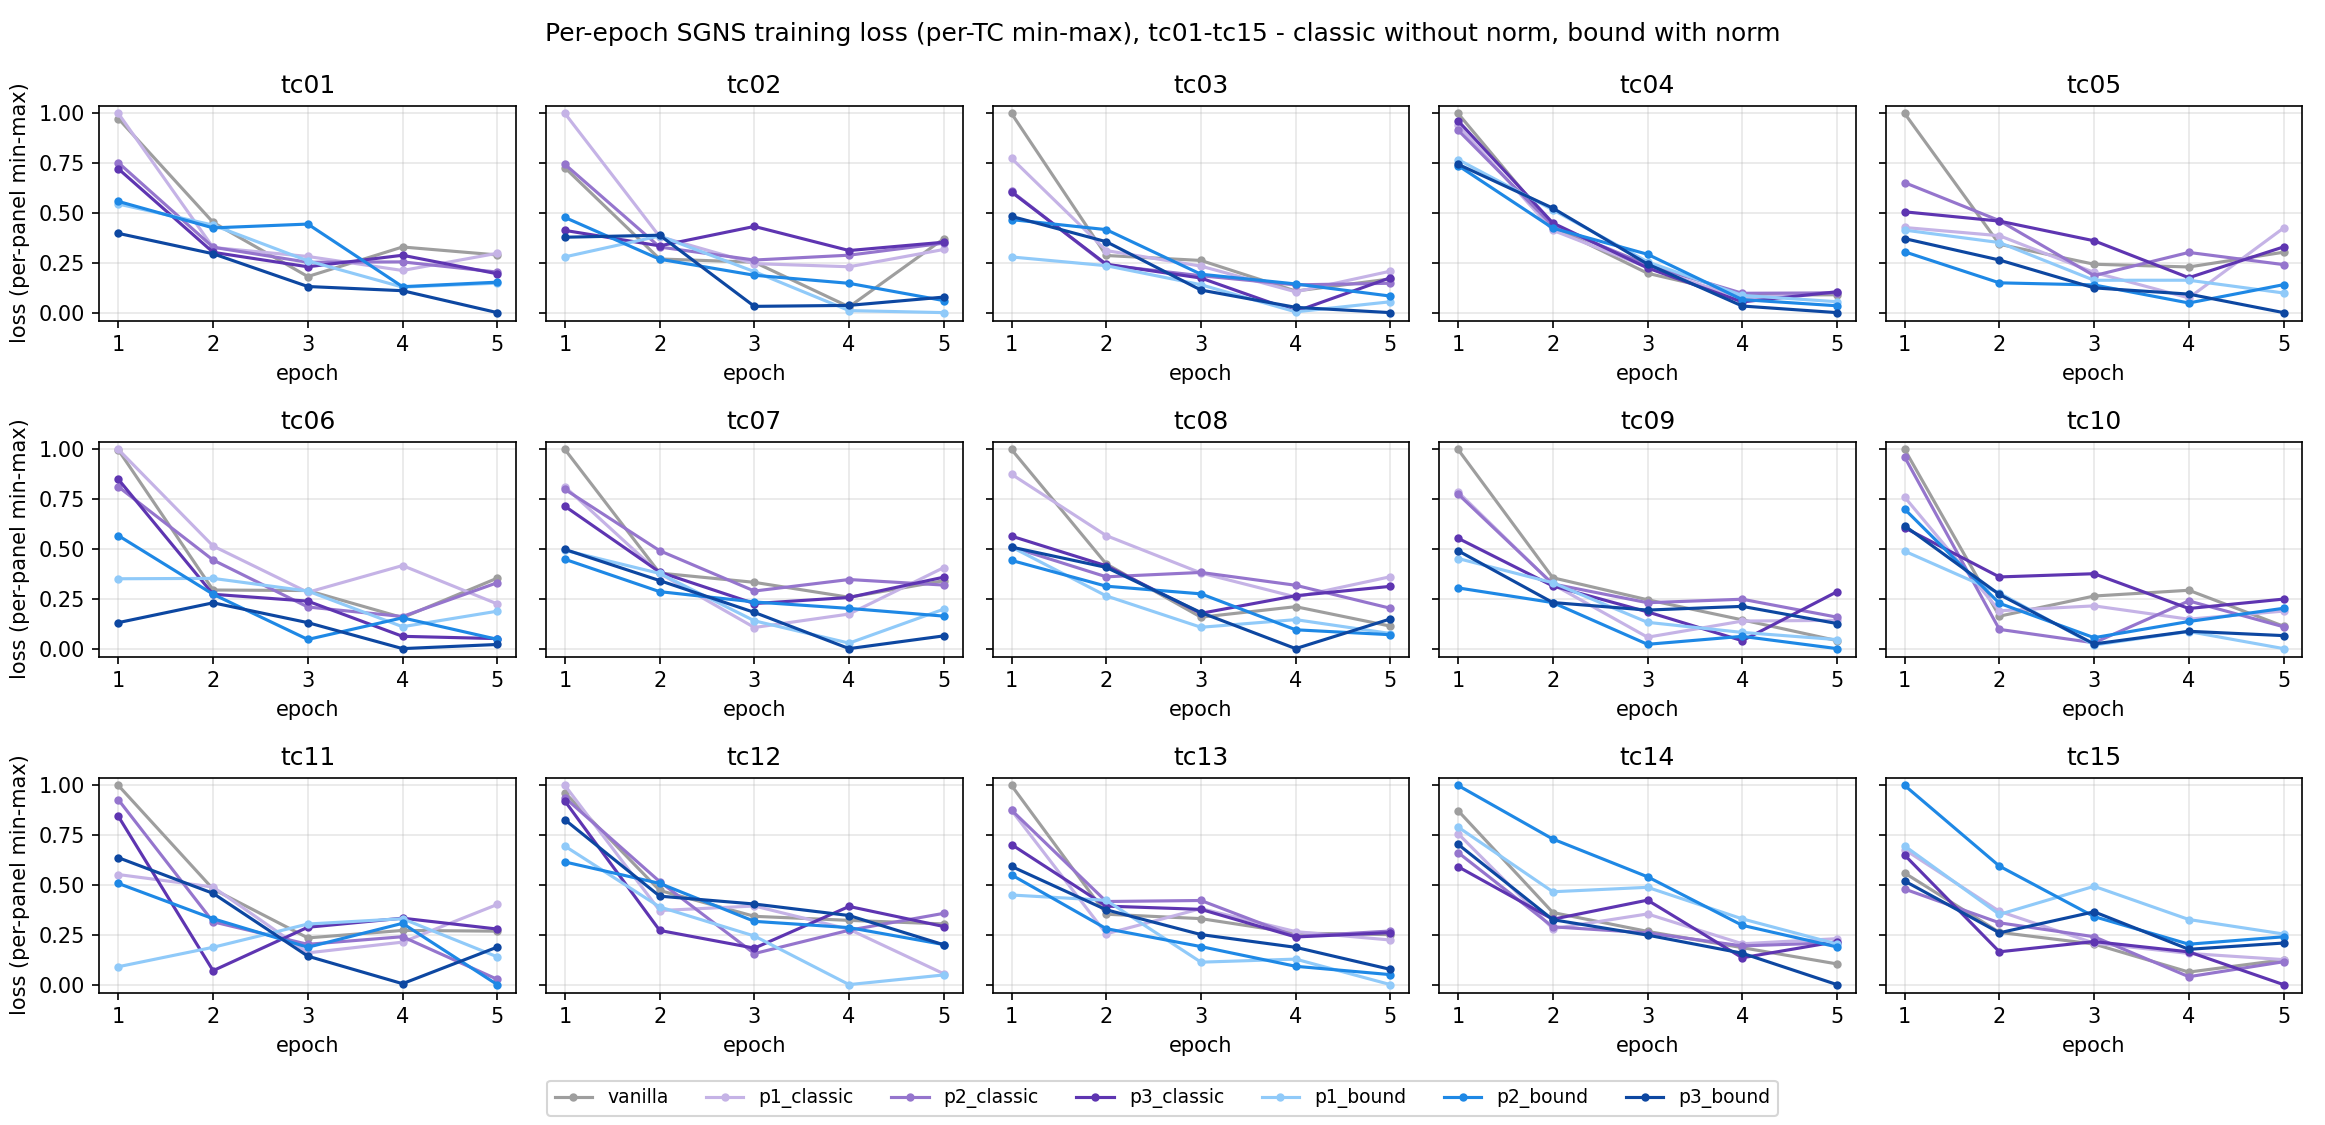
\includegraphics[width=\dimexpr\paperwidth-3cm\relax]{assets/compare/epoch_loss_classic_no-norm_bound_tc01_tc15.png}}
    \caption{Per-epoch RDF2Vec fine-tuning loss on \texttt{tc01}--\texttt{tc15}
    with the raw class-mean classic initialization (no normalization); the bound
    variants are unchanged from Figure~\ref{fig:compare_epoch_loss_tc01_tc15}, and
    the per-panel min--max scaling is the same. Removing the normalization removes
    the saturated start: every classic curve now falls from the first epoch
    onward (a steep initial drop), in contrast to the suppressed and non-monotonic
    classic curves of the normalized run in the main text.}
    \label{fig:norm_ablation_loss_nonorm}
\end{figure}

\section{Per-Test-Case Runtime: Full Results}
\label{app:runtime}

Table~\ref{tab:runtime_per_tc} reports the complete per-test-case runtime
breakdown summarized in Section~\ref{sec:results_runtime}, for every variant on
the synthetic test cases \texttt{tc01}--\texttt{tc12}. Each run is split into the
three pipeline stages -- protograph pretraining, instance-graph initialization
(including the concept-bound construction for the \texttt{*\_bound} variants),
and fine-tuning -- reported separately and as an end-to-end total.

\begin{small}
% Auto-generated by scripts/plot_runtime_per_tc.py
\begin{longtable}{llcccc}
\caption{Per-test-case runtime (seconds), broken into three pipeline stages plus an end-to-end total. Pretraining depends only on the protograph kind (P1/P2/P3) and is shared by the \texttt{classic} and \texttt{bound} variants; the init column includes the concept-bound construction for the \texttt{*\_bound} variants. The \texttt{vanilla} baseline trains from scratch with a random init (only fine-tuning applies). Walk generation and the negligible protograph-creation stage ($\approx$0.02--0.04\,s) are excluded. The final block reports the per-variant mean, excluding tc04 whose much larger walk corpus ($\approx$15$\times$) makes its runtime a far outlier. All RDF2Vec stages were run with 16 worker threads, so the absolute seconds scale with the thread count.}\label{tab:runtime_per_tc}\\
\toprule
 & & & \textbf{Init} & \textbf{Fine-} & \\
\textbf{TC} & \textbf{Variant} & \textbf{Pretrain} & & \textbf{tuning} & \textbf{Total} \\
\midrule
\endfirsthead
\multicolumn{6}{c}{\tablename\ \thetable\ -- continued from previous page}\\
\toprule
 & & & \textbf{Init} & \textbf{Fine-} & \\
\textbf{TC} & \textbf{Variant} & \textbf{Pretrain} & & \textbf{tuning} & \textbf{Total} \\
\midrule
\endhead
\midrule
\multicolumn{6}{r}{\textit{continued on next page}}\\
\endfoot
\bottomrule
\endlastfoot
\multirow{7}{*}{tc01} & \texttt{vanilla} & -- & -- & 15.83 & 15.83 \\*
 & \texttt{p1\_classic} & 0.27 & 0.20 & 15.66 & 16.13 \\*
 & \texttt{p2\_classic} & 2.04 & 0.13 & 15.87 & 18.04 \\*
 & \texttt{p3\_classic} & 1.79 & 0.12 & 18.90 & 20.81 \\*
 & \texttt{p1\_bound} & 0.26 & 1.93 & 17.56 & 19.75 \\*
 & \texttt{p2\_bound} & 2.04 & 2.07 & 17.92 & 22.03 \\*
 & \texttt{p3\_bound} & 1.79 & 2.11 & 17.70 & 21.60 \\
\midrule
\multirow{7}{*}{tc02} & \texttt{vanilla} & -- & -- & 19.05 & 19.05 \\*
 & \texttt{p1\_classic} & 0.32 & 0.13 & 18.19 & 18.64 \\*
 & \texttt{p2\_classic} & 2.42 & 0.13 & 19.12 & 21.67 \\*
 & \texttt{p3\_classic} & 1.85 & 0.13 & 18.99 & 20.97 \\*
 & \texttt{p1\_bound} & 0.32 & 1.94 & 17.69 & 19.95 \\*
 & \texttt{p2\_bound} & 2.42 & 2.15 & 17.53 & 22.10 \\*
 & \texttt{p3\_bound} & 1.85 & 2.11 & 17.68 & 21.64 \\
\midrule
\multirow{7}{*}{tc03} & \texttt{vanilla} & -- & -- & 19.14 & 19.14 \\*
 & \texttt{p1\_classic} & 0.27 & 0.20 & 18.18 & 18.65 \\*
 & \texttt{p2\_classic} & 2.38 & 0.13 & 18.80 & 21.31 \\*
 & \texttt{p3\_classic} & 1.89 & 0.19 & 18.62 & 20.70 \\*
 & \texttt{p1\_bound} & 0.27 & 1.98 & 17.84 & 20.09 \\*
 & \texttt{p2\_bound} & 2.38 & 2.05 & 17.84 & 22.27 \\*
 & \texttt{p3\_bound} & 1.89 & 2.09 & 17.67 & 21.65 \\
\midrule
\multirow{7}{*}{tc04} & \texttt{vanilla} & -- & -- & 286.80 & 286.80 \\*
 & \texttt{p1\_classic} & 0.32 & 1.59 & 276.73 & 278.64 \\*
 & \texttt{p2\_classic} & 1.98 & 1.65 & 279.48 & 283.11 \\*
 & \texttt{p3\_classic} & 1.77 & 1.64 & 280.97 & 284.38 \\*
 & \texttt{p1\_bound} & 0.32 & 24.13 & 275.68 & 300.13 \\*
 & \texttt{p2\_bound} & 1.98 & 25.54 & 283.68 & 311.20 \\*
 & \texttt{p3\_bound} & 1.77 & 26.16 & 290.66 & 318.59 \\
\midrule
\multirow{7}{*}{tc05} & \texttt{vanilla} & -- & -- & 24.96 & 24.96 \\*
 & \texttt{p1\_classic} & 0.29 & 0.15 & 24.41 & 24.85 \\*
 & \texttt{p2\_classic} & 2.48 & 0.15 & 25.08 & 27.71 \\*
 & \texttt{p3\_classic} & 1.95 & 0.14 & 24.82 & 26.91 \\*
 & \texttt{p1\_bound} & 0.29 & 2.40 & 22.94 & 25.63 \\*
 & \texttt{p2\_bound} & 2.48 & 2.67 & 23.32 & 28.47 \\*
 & \texttt{p3\_bound} & 1.95 & 2.63 & 22.88 & 27.46 \\
\midrule
\multirow{7}{*}{tc06} & \texttt{vanilla} & -- & -- & 21.03 & 21.03 \\*
 & \texttt{p1\_classic} & 0.38 & 0.12 & 20.40 & 20.90 \\*
 & \texttt{p2\_classic} & 2.34 & 0.12 & 21.33 & 23.79 \\*
 & \texttt{p3\_classic} & 2.03 & 0.12 & 20.87 & 23.02 \\*
 & \texttt{p1\_bound} & 0.38 & 1.99 & 19.31 & 21.68 \\*
 & \texttt{p2\_bound} & 2.34 & 2.16 & 19.56 & 24.06 \\*
 & \texttt{p3\_bound} & 2.03 & 2.13 & 18.90 & 23.06 \\
\midrule
\multirow{7}{*}{tc07} & \texttt{vanilla} & -- & -- & 24.90 & 24.90 \\*
 & \texttt{p1\_classic} & 0.32 & 0.15 & 23.43 & 23.90 \\*
 & \texttt{p2\_classic} & 2.33 & 0.15 & 24.21 & 26.69 \\*
 & \texttt{p3\_classic} & 1.91 & 0.21 & 24.01 & 26.13 \\*
 & \texttt{p1\_bound} & 0.32 & 2.39 & 22.58 & 25.29 \\*
 & \texttt{p2\_bound} & 2.33 & 2.50 & 23.13 & 27.96 \\*
 & \texttt{p3\_bound} & 1.91 & 2.54 & 22.62 & 27.07 \\
\midrule
\multirow{7}{*}{tc08} & \texttt{vanilla} & -- & -- & 20.60 & 20.60 \\*
 & \texttt{p1\_classic} & 0.36 & 0.13 & 17.79 & 18.28 \\*
 & \texttt{p2\_classic} & 2.38 & 0.12 & 19.25 & 21.75 \\*
 & \texttt{p3\_classic} & 1.94 & 0.12 & 19.12 & 21.18 \\*
 & \texttt{p1\_bound} & 0.36 & 1.96 & 17.99 & 20.31 \\*
 & \texttt{p2\_bound} & 2.38 & 2.10 & 18.20 & 22.68 \\*
 & \texttt{p3\_bound} & 1.94 & 2.20 & 17.94 & 22.08 \\
\midrule
\multirow{7}{*}{tc09} & \texttt{vanilla} & -- & -- & 24.38 & 24.38 \\*
 & \texttt{p1\_classic} & 0.35 & 0.15 & 22.85 & 23.35 \\*
 & \texttt{p2\_classic} & 2.33 & 0.16 & 24.18 & 26.67 \\*
 & \texttt{p3\_classic} & 2.00 & 0.15 & 23.92 & 26.07 \\*
 & \texttt{p1\_bound} & 0.35 & 2.48 & 23.13 & 25.96 \\*
 & \texttt{p2\_bound} & 2.33 & 2.67 & 23.13 & 28.13 \\*
 & \texttt{p3\_bound} & 2.00 & 2.76 & 22.94 & 27.70 \\
\midrule
\multirow{7}{*}{tc10} & \texttt{vanilla} & -- & -- & 22.59 & 22.59 \\*
 & \texttt{p1\_classic} & 0.27 & 0.14 & 21.55 & 21.96 \\*
 & \texttt{p2\_classic} & 2.32 & 0.14 & 22.19 & 24.65 \\*
 & \texttt{p3\_classic} & 2.01 & 0.20 & 22.03 & 24.24 \\*
 & \texttt{p1\_bound} & 0.27 & 2.35 & 20.91 & 23.53 \\*
 & \texttt{p2\_bound} & 2.32 & 2.51 & 21.01 & 25.84 \\*
 & \texttt{p3\_bound} & 2.01 & 2.56 & 20.89 & 25.46 \\
\midrule
\multirow{7}{*}{tc11} & \texttt{vanilla} & -- & -- & 21.09 & 21.09 \\*
 & \texttt{p1\_classic} & 0.32 & 0.14 & 20.41 & 20.87 \\*
 & \texttt{p2\_classic} & 2.37 & 0.13 & 21.10 & 23.60 \\*
 & \texttt{p3\_classic} & 1.80 & 0.13 & 21.12 & 23.05 \\*
 & \texttt{p1\_bound} & 0.32 & 2.14 & 19.41 & 21.87 \\*
 & \texttt{p2\_bound} & 2.37 & 2.31 & 19.97 & 24.65 \\*
 & \texttt{p3\_bound} & 1.80 & 2.40 & 20.10 & 24.30 \\
\midrule
\multirow{7}{*}{tc12} & \texttt{vanilla} & -- & -- & 28.66 & 28.66 \\*
 & \texttt{p1\_classic} & 0.25 & 0.18 & 27.71 & 28.14 \\*
 & \texttt{p2\_classic} & 2.40 & 0.18 & 28.35 & 30.93 \\*
 & \texttt{p3\_classic} & 1.83 & 0.18 & 28.08 & 30.09 \\*
 & \texttt{p1\_bound} & 0.25 & 2.95 & 26.91 & 30.11 \\*
 & \texttt{p2\_bound} & 2.40 & 3.14 & 26.66 & 32.20 \\*
 & \texttt{p3\_bound} & 1.83 & 3.22 & 26.64 & 31.69 \\
\midrule
\multirow{7}{*}{mean} & \texttt{vanilla} & -- & -- & 22.02 & 22.02 \\*
 & \texttt{p1\_classic} & 0.31 & 0.15 & 20.96 & 21.42 \\*
 & \texttt{p2\_classic} & 2.34 & 0.14 & 21.77 & 24.26 \\*
 & \texttt{p3\_classic} & 1.91 & 0.15 & 21.86 & 23.92 \\*
 & \texttt{p1\_bound} & 0.31 & 2.23 & 20.57 & 23.11 \\*
 & \texttt{p2\_bound} & 2.34 & 2.39 & 20.75 & 25.49 \\*
 & \texttt{p3\_bound} & 1.91 & 2.43 & 20.54 & 24.88 \\
\end{longtable}

\end{small}

\section{GEval Downstream-Task Plots}
\label{app:geval-plots}

This appendix collects the per-task GEval plots referenced from
Section~\ref{sec:dbpedia_geval}. All plots compare the same fine-tuned DBpedia
variants: \texttt{vanilla}, the classic transfer
(\texttt{p1}/\texttt{p2}/\texttt{p3}), and the norm-capped concept-bound init
(\texttt{p2}/\texttt{p3}~\texttt{cap16}). Figures~\ref{fig:geval_clustering},
\ref{fig:geval_classification}, and~\ref{fig:geval_analogies} cover the
clustering, classification, and semantic-analogy tasks discussed in the main
text.

\begin{figure}[ht]
  \centering
  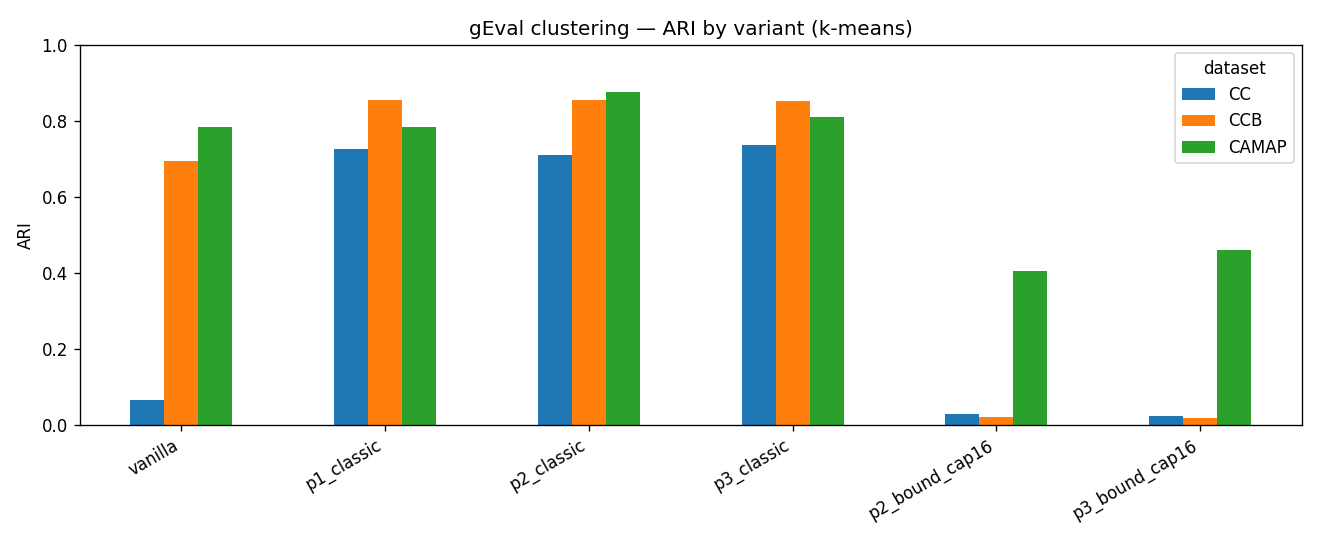
\includegraphics[width=0.85\textwidth]{assets/dbpedia/geval/clustering_ari.png}
  \caption{GEval clustering: adjusted Rand index (ARI) by variant on the CC, CCB,
  and CAMAP gold standards (k-means, $k$ = number of gold classes). The classic
  transfer dominates; the capped bound stays at the \texttt{vanilla} floor on the
  shared-parent tasks (CC/CCB) and recovers only partially on CAMAP.}
  \label{fig:geval_clustering}
\end{figure}

\begin{figure}[ht]
  \centering
  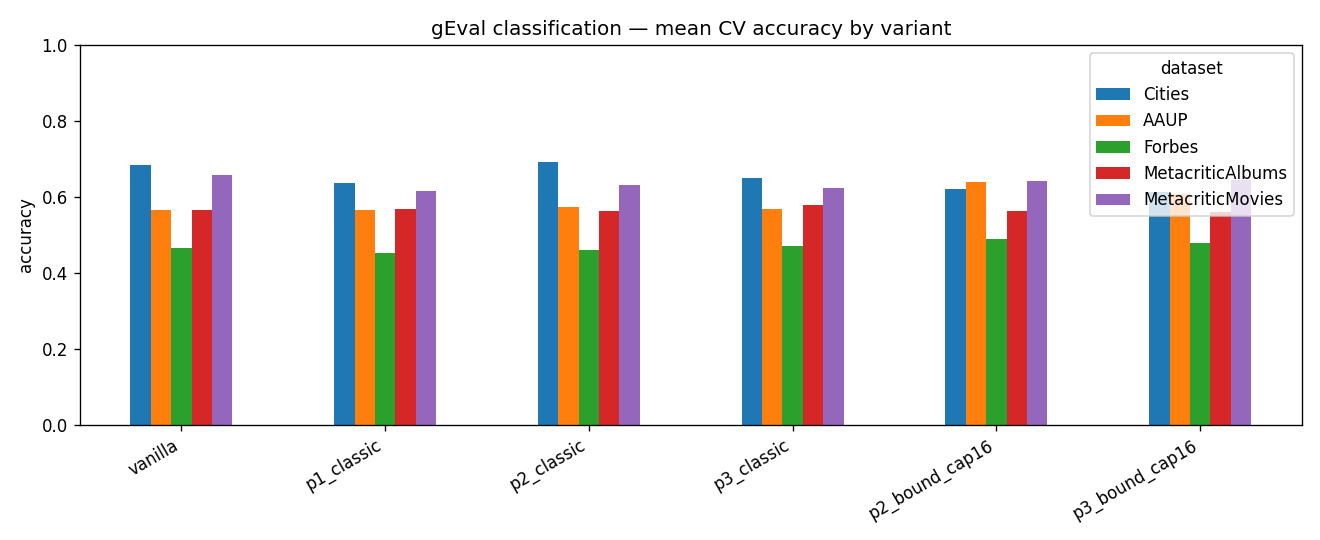
\includegraphics[width=0.85\textwidth]{assets/dbpedia/geval/classification_acc.png}
  \caption{GEval classification: mean 10-fold cross-validated accuracy by variant
  across five datasets (averaged over the naive Bayes, $k$-NN, decision-tree, and
  linear-SVM classifiers). The variants flatten once a classifier does the
  separating; no initialization dominates.}
  \label{fig:geval_classification}
\end{figure}

\begin{figure}[ht]
  \centering
  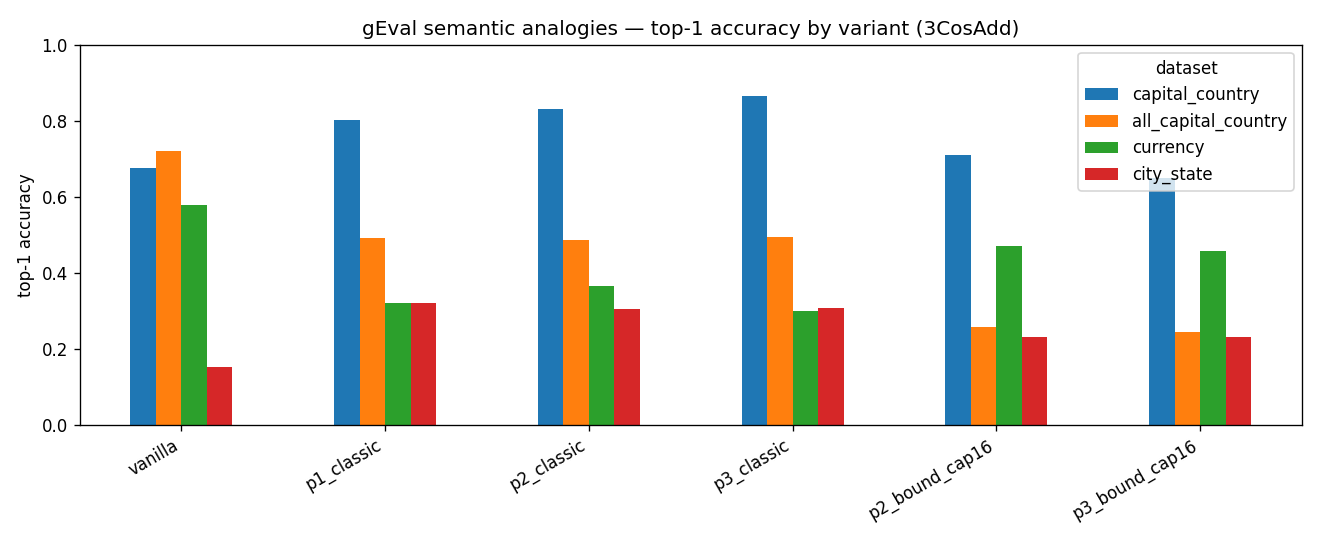
\includegraphics[width=0.85\textwidth]{assets/dbpedia/geval/analogies_top1.png}
  \caption{GEval semantic analogies: top-1 accuracy by variant on four relation
  sets (3CosAdd over the full vocabulary). The classic transfer wins on the
  small capital-country and city-state sets but loses to \texttt{vanilla} on the
  larger all-capital-country and currency sets.}
  \label{fig:geval_analogies}
\end{figure}

\backmatter

\chapter{Ehrenwörtliche Erklärung}

Ich versichere, dass ich die beiliegende Bachelor-, Master-, Seminar-, oder
Projektarbeit ohne Hilfe Dritter und ohne Benutzung anderer als der angegebenen
Quellen und in der untenstehenden Tabelle angegebenen Hilfsmittel angefertigt
und die den benutzten Quellen wörtlich oder inhaltlich entnommenen Stellen als
solche kenntlich gemacht habe. Diese Arbeit hat in gleicher oder ähnlicher Form
noch keiner Prüfungsbehörde vorgelegen. Ich bin mir bewusst, dass eine falsche
Erklärung rechtliche Folgen haben wird.

% Declare below which AI tools you used in the process of writing your work,
% including text, image, code, and data generation. If you used a tool for a
% purpose not included in the list yet, add it to the list.
\begin{center}
  \textbf{Declaration of Used AI Tools} \\[.3em]
  \begin{tabularx}{\textwidth}{lXlc}
    \toprule
    Tool & Purpose & Where? & Useful? \\
    \midrule
    Claude & Rephrasing & Throughout & +++ \\
    ChatGPT & Structure of the related-work chapter & Ch.~\ref{ch:related_work} & + \\
    Claude Opus & Diagram generation & Ch.~\ref{ch:background}, \ref{ch:classic} & +++ \\
    Claude Sonnet & Training scripts & Throughout & +++ \\
    Claude Opus & Ideas for the normalization and capping schemes & Ch.~\ref{ch:classic}, \ref{ch:experiments} & +++ \\
    \bottomrule
  \end{tabularx}
\end{center}

\vspace{2cm}
\noindent Unterschrift\\
\noindent Mannheim, den 18.~Juni 2026 \hfill

\end{document}
